% Options for packages loaded elsewhere
\PassOptionsToPackage{unicode}{hyperref}
\PassOptionsToPackage{hyphens}{url}
\PassOptionsToPackage{dvipsnames,svgnames,x11names}{xcolor}
%
\documentclass[
  letterpaper,
  DIV=11,
  numbers=noendperiod]{scrreprt}

\usepackage{amsmath,amssymb}
\usepackage{iftex}
\ifPDFTeX
  \usepackage[T1]{fontenc}
  \usepackage[utf8]{inputenc}
  \usepackage{textcomp} % provide euro and other symbols
\else % if luatex or xetex
  \usepackage{unicode-math}
  \defaultfontfeatures{Scale=MatchLowercase}
  \defaultfontfeatures[\rmfamily]{Ligatures=TeX,Scale=1}
\fi
\usepackage{lmodern}
\ifPDFTeX\else  
    % xetex/luatex font selection
\fi
% Use upquote if available, for straight quotes in verbatim environments
\IfFileExists{upquote.sty}{\usepackage{upquote}}{}
\IfFileExists{microtype.sty}{% use microtype if available
  \usepackage[]{microtype}
  \UseMicrotypeSet[protrusion]{basicmath} % disable protrusion for tt fonts
}{}
\makeatletter
\@ifundefined{KOMAClassName}{% if non-KOMA class
  \IfFileExists{parskip.sty}{%
    \usepackage{parskip}
  }{% else
    \setlength{\parindent}{0pt}
    \setlength{\parskip}{6pt plus 2pt minus 1pt}}
}{% if KOMA class
  \KOMAoptions{parskip=half}}
\makeatother
\usepackage{xcolor}
\setlength{\emergencystretch}{3em} % prevent overfull lines
\setcounter{secnumdepth}{5}
% Make \paragraph and \subparagraph free-standing
\makeatletter
\ifx\paragraph\undefined\else
  \let\oldparagraph\paragraph
  \renewcommand{\paragraph}{
    \@ifstar
      \xxxParagraphStar
      \xxxParagraphNoStar
  }
  \newcommand{\xxxParagraphStar}[1]{\oldparagraph*{#1}\mbox{}}
  \newcommand{\xxxParagraphNoStar}[1]{\oldparagraph{#1}\mbox{}}
\fi
\ifx\subparagraph\undefined\else
  \let\oldsubparagraph\subparagraph
  \renewcommand{\subparagraph}{
    \@ifstar
      \xxxSubParagraphStar
      \xxxSubParagraphNoStar
  }
  \newcommand{\xxxSubParagraphStar}[1]{\oldsubparagraph*{#1}\mbox{}}
  \newcommand{\xxxSubParagraphNoStar}[1]{\oldsubparagraph{#1}\mbox{}}
\fi
\makeatother

\usepackage{color}
\usepackage{fancyvrb}
\newcommand{\VerbBar}{|}
\newcommand{\VERB}{\Verb[commandchars=\\\{\}]}
\DefineVerbatimEnvironment{Highlighting}{Verbatim}{commandchars=\\\{\}}
% Add ',fontsize=\small' for more characters per line
\usepackage{framed}
\definecolor{shadecolor}{RGB}{241,243,245}
\newenvironment{Shaded}{\begin{snugshade}}{\end{snugshade}}
\newcommand{\AlertTok}[1]{\textcolor[rgb]{0.68,0.00,0.00}{#1}}
\newcommand{\AnnotationTok}[1]{\textcolor[rgb]{0.37,0.37,0.37}{#1}}
\newcommand{\AttributeTok}[1]{\textcolor[rgb]{0.40,0.45,0.13}{#1}}
\newcommand{\BaseNTok}[1]{\textcolor[rgb]{0.68,0.00,0.00}{#1}}
\newcommand{\BuiltInTok}[1]{\textcolor[rgb]{0.00,0.23,0.31}{#1}}
\newcommand{\CharTok}[1]{\textcolor[rgb]{0.13,0.47,0.30}{#1}}
\newcommand{\CommentTok}[1]{\textcolor[rgb]{0.37,0.37,0.37}{#1}}
\newcommand{\CommentVarTok}[1]{\textcolor[rgb]{0.37,0.37,0.37}{\textit{#1}}}
\newcommand{\ConstantTok}[1]{\textcolor[rgb]{0.56,0.35,0.01}{#1}}
\newcommand{\ControlFlowTok}[1]{\textcolor[rgb]{0.00,0.23,0.31}{\textbf{#1}}}
\newcommand{\DataTypeTok}[1]{\textcolor[rgb]{0.68,0.00,0.00}{#1}}
\newcommand{\DecValTok}[1]{\textcolor[rgb]{0.68,0.00,0.00}{#1}}
\newcommand{\DocumentationTok}[1]{\textcolor[rgb]{0.37,0.37,0.37}{\textit{#1}}}
\newcommand{\ErrorTok}[1]{\textcolor[rgb]{0.68,0.00,0.00}{#1}}
\newcommand{\ExtensionTok}[1]{\textcolor[rgb]{0.00,0.23,0.31}{#1}}
\newcommand{\FloatTok}[1]{\textcolor[rgb]{0.68,0.00,0.00}{#1}}
\newcommand{\FunctionTok}[1]{\textcolor[rgb]{0.28,0.35,0.67}{#1}}
\newcommand{\ImportTok}[1]{\textcolor[rgb]{0.00,0.46,0.62}{#1}}
\newcommand{\InformationTok}[1]{\textcolor[rgb]{0.37,0.37,0.37}{#1}}
\newcommand{\KeywordTok}[1]{\textcolor[rgb]{0.00,0.23,0.31}{\textbf{#1}}}
\newcommand{\NormalTok}[1]{\textcolor[rgb]{0.00,0.23,0.31}{#1}}
\newcommand{\OperatorTok}[1]{\textcolor[rgb]{0.37,0.37,0.37}{#1}}
\newcommand{\OtherTok}[1]{\textcolor[rgb]{0.00,0.23,0.31}{#1}}
\newcommand{\PreprocessorTok}[1]{\textcolor[rgb]{0.68,0.00,0.00}{#1}}
\newcommand{\RegionMarkerTok}[1]{\textcolor[rgb]{0.00,0.23,0.31}{#1}}
\newcommand{\SpecialCharTok}[1]{\textcolor[rgb]{0.37,0.37,0.37}{#1}}
\newcommand{\SpecialStringTok}[1]{\textcolor[rgb]{0.13,0.47,0.30}{#1}}
\newcommand{\StringTok}[1]{\textcolor[rgb]{0.13,0.47,0.30}{#1}}
\newcommand{\VariableTok}[1]{\textcolor[rgb]{0.07,0.07,0.07}{#1}}
\newcommand{\VerbatimStringTok}[1]{\textcolor[rgb]{0.13,0.47,0.30}{#1}}
\newcommand{\WarningTok}[1]{\textcolor[rgb]{0.37,0.37,0.37}{\textit{#1}}}

\providecommand{\tightlist}{%
  \setlength{\itemsep}{0pt}\setlength{\parskip}{0pt}}\usepackage{longtable,booktabs,array}
\usepackage{calc} % for calculating minipage widths
% Correct order of tables after \paragraph or \subparagraph
\usepackage{etoolbox}
\makeatletter
\patchcmd\longtable{\par}{\if@noskipsec\mbox{}\fi\par}{}{}
\makeatother
% Allow footnotes in longtable head/foot
\IfFileExists{footnotehyper.sty}{\usepackage{footnotehyper}}{\usepackage{footnote}}
\makesavenoteenv{longtable}
\usepackage{graphicx}
\makeatletter
\def\maxwidth{\ifdim\Gin@nat@width>\linewidth\linewidth\else\Gin@nat@width\fi}
\def\maxheight{\ifdim\Gin@nat@height>\textheight\textheight\else\Gin@nat@height\fi}
\makeatother
% Scale images if necessary, so that they will not overflow the page
% margins by default, and it is still possible to overwrite the defaults
% using explicit options in \includegraphics[width, height, ...]{}
\setkeys{Gin}{width=\maxwidth,height=\maxheight,keepaspectratio}
% Set default figure placement to htbp
\makeatletter
\def\fps@figure{htbp}
\makeatother
% definitions for citeproc citations
\NewDocumentCommand\citeproctext{}{}
\NewDocumentCommand\citeproc{mm}{%
  \begingroup\def\citeproctext{#2}\cite{#1}\endgroup}
\makeatletter
 % allow citations to break across lines
 \let\@cite@ofmt\@firstofone
 % avoid brackets around text for \cite:
 \def\@biblabel#1{}
 \def\@cite#1#2{{#1\if@tempswa , #2\fi}}
\makeatother
\newlength{\cslhangindent}
\setlength{\cslhangindent}{1.5em}
\newlength{\csllabelwidth}
\setlength{\csllabelwidth}{3em}
\newenvironment{CSLReferences}[2] % #1 hanging-indent, #2 entry-spacing
 {\begin{list}{}{%
  \setlength{\itemindent}{0pt}
  \setlength{\leftmargin}{0pt}
  \setlength{\parsep}{0pt}
  % turn on hanging indent if param 1 is 1
  \ifodd #1
   \setlength{\leftmargin}{\cslhangindent}
   \setlength{\itemindent}{-1\cslhangindent}
  \fi
  % set entry spacing
  \setlength{\itemsep}{#2\baselineskip}}}
 {\end{list}}
\usepackage{calc}
\newcommand{\CSLBlock}[1]{\hfill\break\parbox[t]{\linewidth}{\strut\ignorespaces#1\strut}}
\newcommand{\CSLLeftMargin}[1]{\parbox[t]{\csllabelwidth}{\strut#1\strut}}
\newcommand{\CSLRightInline}[1]{\parbox[t]{\linewidth - \csllabelwidth}{\strut#1\strut}}
\newcommand{\CSLIndent}[1]{\hspace{\cslhangindent}#1}

\KOMAoption{captions}{tableheading}
\makeatletter
\@ifpackageloaded{tcolorbox}{}{\usepackage[skins,breakable]{tcolorbox}}
\@ifpackageloaded{fontawesome5}{}{\usepackage{fontawesome5}}
\definecolor{quarto-callout-color}{HTML}{909090}
\definecolor{quarto-callout-note-color}{HTML}{0758E5}
\definecolor{quarto-callout-important-color}{HTML}{CC1914}
\definecolor{quarto-callout-warning-color}{HTML}{EB9113}
\definecolor{quarto-callout-tip-color}{HTML}{00A047}
\definecolor{quarto-callout-caution-color}{HTML}{FC5300}
\definecolor{quarto-callout-color-frame}{HTML}{acacac}
\definecolor{quarto-callout-note-color-frame}{HTML}{4582ec}
\definecolor{quarto-callout-important-color-frame}{HTML}{d9534f}
\definecolor{quarto-callout-warning-color-frame}{HTML}{f0ad4e}
\definecolor{quarto-callout-tip-color-frame}{HTML}{02b875}
\definecolor{quarto-callout-caution-color-frame}{HTML}{fd7e14}
\makeatother
\makeatletter
\@ifpackageloaded{bookmark}{}{\usepackage{bookmark}}
\makeatother
\makeatletter
\@ifpackageloaded{caption}{}{\usepackage{caption}}
\AtBeginDocument{%
\ifdefined\contentsname
  \renewcommand*\contentsname{Table of contents}
\else
  \newcommand\contentsname{Table of contents}
\fi
\ifdefined\listfigurename
  \renewcommand*\listfigurename{List of Figures}
\else
  \newcommand\listfigurename{List of Figures}
\fi
\ifdefined\listtablename
  \renewcommand*\listtablename{List of Tables}
\else
  \newcommand\listtablename{List of Tables}
\fi
\ifdefined\figurename
  \renewcommand*\figurename{Figure}
\else
  \newcommand\figurename{Figure}
\fi
\ifdefined\tablename
  \renewcommand*\tablename{Table}
\else
  \newcommand\tablename{Table}
\fi
}
\@ifpackageloaded{float}{}{\usepackage{float}}
\floatstyle{ruled}
\@ifundefined{c@chapter}{\newfloat{codelisting}{h}{lop}}{\newfloat{codelisting}{h}{lop}[chapter]}
\floatname{codelisting}{Listing}
\newcommand*\listoflistings{\listof{codelisting}{List of Listings}}
\makeatother
\makeatletter
\makeatother
\makeatletter
\@ifpackageloaded{caption}{}{\usepackage{caption}}
\@ifpackageloaded{subcaption}{}{\usepackage{subcaption}}
\makeatother

\ifLuaTeX
  \usepackage{selnolig}  % disable illegal ligatures
\fi
\usepackage{bookmark}

\IfFileExists{xurl.sty}{\usepackage{xurl}}{} % add URL line breaks if available
\urlstyle{same} % disable monospaced font for URLs
\hypersetup{
  pdftitle={Open Science: Wie sich die Wissenschaft öffnet},
  pdfauthor={Lukas Röseler},
  colorlinks=true,
  linkcolor={blue},
  filecolor={Maroon},
  citecolor={Blue},
  urlcolor={Blue},
  pdfcreator={LaTeX via pandoc}}


\title{Open Science: Wie sich die Wissenschaft öffnet}
\author{Lukas Röseler}
\date{}

\begin{document}
\maketitle

\renewcommand*\contentsname{Table of contents}
{
\hypersetup{linkcolor=}
\setcounter{tocdepth}{2}
\tableofcontents
}

\bookmarksetup{startatroot}

\chapter{Willkommen}\label{willkommen}

\bookmarksetup{startatroot}

\chapter*{Willkommen}\label{willkommen-1}
\addcontentsline{toc}{chapter}{Willkommen}

\markboth{Willkommen}{Willkommen}

\begin{tcolorbox}[enhanced jigsaw, title=\textcolor{quarto-callout-caution-color}{\faFire}\hspace{0.5em}{Warnung}, colbacktitle=quarto-callout-caution-color!10!white, rightrule=.15mm, titlerule=0mm, left=2mm, bottomrule=.15mm, arc=.35mm, leftrule=.75mm, toprule=.15mm, opacityback=0, breakable, bottomtitle=1mm, colframe=quarto-callout-caution-color-frame, toptitle=1mm, opacitybacktitle=0.6, coltitle=black, colback=white]

Dieses Projekt befindet sich in Arbeit und ist aktuell noch unfertig!
Texte sind unvollständig oder fehlen, Quellenangaben und Abbildungen
sind vorläufig, und es wimmelt von Rechtschreibfelehrn\ldots{}

\end{tcolorbox}

Viele wissenschaftliche Disziplinen haben sich in den letzten Jahren
stark verändert. Neue Zeitschriften, Methoden, Initiativen,
Gesellschaften, Strukturen, und vieles mehr sind entstanden. Es ist die
Rede von einer Krise (Mede et al. 2020), einer Revolution (Brian A.
Nosek et al. 2018) oder einer Renaissance (L. D. Nelson, Simmons, and
Simonsohn 2018.). All diese Veränderungen haben gemeinsam zu einem
stärkeren Grad an Offenheit und Transparenz geführt und das
Wissenschaftssystem maßgeblich verändert.

In diesem Buch werden niedrigschwellig der Begriff der Offenheit, die
Ursprünge des Wandels, und die Open Science Bewegung erklärt. Es werden
Hintergründe des wissenschaftlichen Systems, neu entwickelte Methoden,
und Probleme amtierender Methoden erläutert. Dabei wird vorwiegend auf
Beispiele und Entwicklungen aus der Psychologie zurückgegriffen.

\section{Literatur}\label{literatur}

\bookmarksetup{startatroot}

\chapter{Über das Buch}\label{uxfcber-das-buch}

Wissenschaft wird zu einem Maßgeblichen Teil von den Mitgliedern einer
Gesellschaft finanziert, beispielsweise über Steuergelder. Das bedeutet,
eine Gemeinschaft fördert einzelne Personen, um ein tieferes Verständnis
von sich und der Welt zu erlangen und im Gegenzug Unterstützung bei der
Lösung verschiedener Probleme zu erhalten. Dadurch sind
Wissenschaftler*innen der Gesellschaft in einem gewissen Maße
Rechenschaft schuldig. Dabei geht es nicht darum, dass jede
wissenschaftliche Erkenntnis notwendigerweise Früchte tragen muss, aber,
dass sie wissenschaftlichen Qualitätskriterien entspricht und zumindest
für andere Forschende nachvollziehbar und nachprüfbar ist. Inwiefern das
in verschiedenen Disziplinen der Fall ist und wie Personen sich dafür
einsetzen, diese Rechenschaft zu ermöglichen, möchte ich in diesem Buch
darlegen.

Dieses Buch soll selbst ein Teil der offenen Wissenschaft sein. Im
Kontext der Probleme und Lösungen erkläre ich, wie der Beruf
\emph{Wissenschaftler*in} aussieht, wie das Wissenschaftssystem
funktioniert, und erörtere an Beispielen auszugsweise wissenschaftliche
Debatten. Zur Offenheit gehört auch, dass das Buch frei zugänglich ist.

\begin{tcolorbox}[enhanced jigsaw, title=\textcolor{quarto-callout-note-color}{\faInfo}\hspace{0.5em}{Danksagungen}, colbacktitle=quarto-callout-note-color!10!white, rightrule=.15mm, titlerule=0mm, left=2mm, bottomrule=.15mm, arc=.35mm, leftrule=.75mm, toprule=.15mm, opacityback=0, breakable, bottomtitle=1mm, colframe=quarto-callout-note-color-frame, toptitle=1mm, opacitybacktitle=0.6, coltitle=black, colback=white]

Dieses Buch wäre nicht möglich gewesen ohne die Unterstützung meiner
Frau Jessica. Von ihr nährt sich mein Optimismus und meine Kraft, mich
für eine offene, nachvollziehbare, und gerechte Wissenschaft
einzusetzen.

In Beispielen, Hinweisen, und Anmerkungen stütze ich mich zudem auf
zahlreiche Beispiele, die ich mit Kolleginnen, Kollegen, Freundinnen und
Freunden diskutiert habe. Ich danke Daniel Wolf, Johannes Leder,
Matthias Borgstede, Astrid Schütz, Ulrike Starker, Georg Felser, Viola
Voß, Mitja Back, Jan H. Höffler und vielen anderen für die spannenden
Gespräche!

\end{tcolorbox}

\begin{tcolorbox}[enhanced jigsaw, title=\textcolor{quarto-callout-note-color}{\faInfo}\hspace{0.5em}{Über mich}, colbacktitle=quarto-callout-note-color!10!white, rightrule=.15mm, titlerule=0mm, left=2mm, bottomrule=.15mm, arc=.35mm, leftrule=.75mm, toprule=.15mm, opacityback=0, breakable, bottomtitle=1mm, colframe=quarto-callout-note-color-frame, toptitle=1mm, opacitybacktitle=0.6, coltitle=black, colback=white]

Mein Name ist Lukas Röseler und ich bin Wissenschaftler. Ich habe in
Wernigerode Wirtschaftspsychologie studiert, mich darüber hinaus mit
Philosophie und Wissenschaftstheorie beschäftigt, und habe 2021 als
Doktorand der ersten Generation\footnotemark{} in Bamberg meinen
Doktortitel in Psychologie erhalten. Seit 2023 bin ich Geschäftsführer
des Münster Center for Open Science und darf mich im Rahmen dessen mit
transparenter und vertrauenswürdiger Wissenschaft in zahlreichen
Disziplinen auseinandersetzen. Parallel dazu betreibe ich
Meta-Wissenschaft, also \emph{Wissenschaft über Wissenschaft}.

Ich habe dieses Buch geschrieben, um das Thema \emph{Open Science}
anderen Wissenschaftler*innen, Studierenden, und allen anderen Personen
auf einem einfachen aber ausführlichen Niveau zu erklären. Ein großer
Aspekt von offener Wissenschaft ist nämlich, dass auch Personen, die
primär nichts mit Wissenschaft zu tun haben, zumindest teilweise
verstehen können, was dort vor sich geht. Das gleicht einem Schloss, das
einst nur den reichen Herrschenden zugänglich war, im Zuge eines
Gesellschaftlichen Wandels nun offene Tore und Türen hat und für alle
frei zur Besichtigung steht.

Angesichts dieses Zieles veröffentliche ich das Buch kostenlos und
stelle es online zur Verfügung. Sie können mir
\href{https://docs.google.com/forms/d/1Ce4uyr8bRSHZ5yywP3TPdIg8XMLxZqE-mYVL82K6QHI}{hier}
anonym Rückmeldung geben (Betreff: ``Open Science Buch'').

\begin{figure}[H]

{\centering 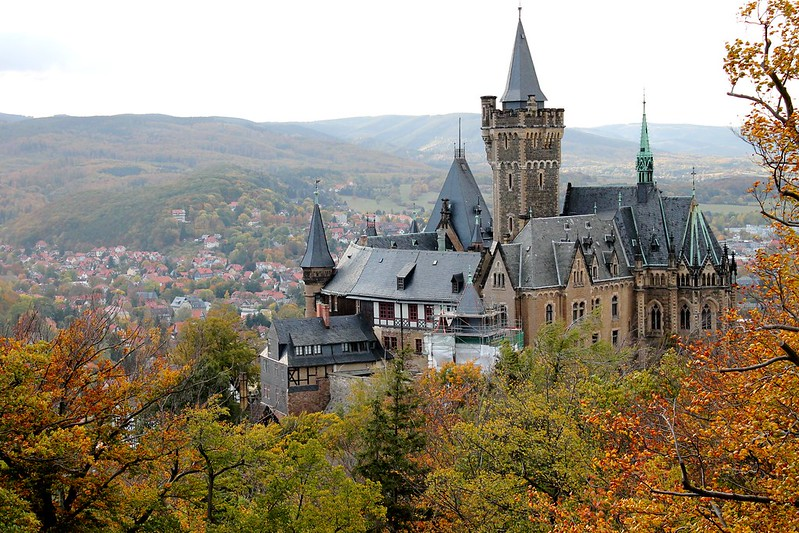
\includegraphics[width=6.25in,height=\textheight]{images/wernigerode.jpg}

}

\caption{Blick über Wernigerode}

\end{figure}%

\end{tcolorbox}

\footnotetext{Das bedeutet, dass meine (Groß-)eltern keine Doktortitel
haben.}

\part{Einleitung}

\section*{Einleitung}\label{einleitung-1}
\addcontentsline{toc}{section}{Einleitung}

\markright{Einleitung}

\part{Überschrift passend zum Beispiel}

-~~~~~~~~~ Beispiel, bei dem Psychologische Wissenschaft wichtig ist

-~~~~~~~~~ Befunde aus der Wissenschaft zitieren

-~~~~~~~~~ Diese Befunde sind eventuell falsch

-~~~~~~~~~ Wie finden wir heraus, ob sie falsch sind?

-~~~~~~~~~ Wie stark können wir uns darauf verlassen?

-~~~~~~~~~ Wie stellen wir sicher, dass wir uns stärker auf Wissenschaft
verlassen können?

\hyperref[_ftnref2]{{[}2{]}} Durch die Ungewissheit über genaue Ursachen
von geringen Replikationsraten wird teilweise auch eher zu dem Begriff
„Vertrauenskrise'' geraten (z.B. Feest, 2023).

~\hyperref[_msoanchor_1]{{[}LR1{]}}hier noch Wissenschaftsskepsis
erwähnen: \url{https://osf.io/preprints/psyarxiv/7u4fg} ~

~\hyperref[_msoanchor_2]{{[}LR2{]}}OS Taxonomie:
\url{https://periodicos.ufsc.br/index.php/eb/article/view/91712}

Bild

\url{https://zenodo.org/records/7940641}

~\hyperref[_msoanchor_3]{{[}LR3{]}}\url{https://www.researchgate.net/publication/374381552_What_is_the_Replication_Crisis_a_Crisis_of}

~\hyperref[_msoanchor_4]{{[}LR4{]}}hier Bild vom Spektrum und der
Verortung dieses Buches hintun; evtl. Umfrageergebnisse von
Wissenschaftler*innen dazutun und zitieren, da gibt es was

~\hyperref[_msoanchor_5]{{[}LR5{]}}Als Infobox

\section*{Literatur}\label{literatur-1}
\addcontentsline{toc}{section}{Literatur}

\markright{Literatur}

\chapter{Was ist Open Science?}\label{was-ist-open-science}

In der Wissenschaft dreht es sich oft um Details: Was genau passierte in
der Studie? Welche Bilder sahen Versuchspersonen auf was für einem
Bildschirm? Was war die Bildwiederholungsrate des Bildschirmes, und
waren die Farben dabei mittels Spektralphotometer kalibriert?
Wissenschaftliche Untersuchungen und ihre Befunde werden heutzutage in
Zeitschriftenartikeln beschrieben. Es kommt nicht selten vor, dass darin
eines der oben aufgeführten Details fehlt, in den Zusatzmaterialien
nicht auffindbar ist, oder die Autor*innen nicht gefragt werden können,
weil ihre E-Mail-Adresse nicht mehr aktuell ist. Wenn nun aber der
Befund von genauso einem Detail abhängt, werden zukünftige Forschende
Probleme haben, ihn zum Vorschein zu bringen. Auf dieser konkreten Ebene
bedeutet Open Science die Möglichkeit für jede Person, im Rahmen von
ethischen und legalen Einschränkungen (z.B. Anonymität), detaillierte
Einsicht in den gesamten wissenschaftlichen Prozess der
Erkenntnisgewinnung zu erhalten. Es sollte also genau beschrieben
werden, wie die Untersuchung ablief, welche Materialien dafür verwendet
werden, welche Daten daraus resultierten, wie diese weiterverarbeitet
und ausgewertet wurden, und schließlich, was daraus zu lernen ist.

Auf einer abstrakten Ebene meint Open Science einen höheren Grad an
Offenheit und Transparenz in allen Facetten der Wissenschaft. Dazu
gehören wie beschrieben Studienmaterialien (z.B. Fragebögen, Bilder,
oder Videos), der wissenschaftliche Bericht, oder der Diskurs im Rahmen
der Begutachtung wissenschaftlicher Berichte durch ihre Kolleg*innen
(Peer-Review). Aber auch auf der systemischen Ebene kann der Grad an
Transparenz steigen: Beispielsweise gibt es Listen mit Zeitschriften
(\url{https://doaj.org}) oder Listen mit Professuren in einem bestimmten
Wissenschaftsbereich (z.B. für die
\href{https://docs.google.com/spreadsheets/d/1XwO4n88zkdH1bDGpW6Uz8f4sH24P5FG0ihUp7i0Y-gY/edit\#gid=1684024252}{Persönlichkeitspsychologie
in Deutschland}). Schließlich kann mit Offenheit auch die Durchführung
einer Konferenz im „hybriden Format'', also an einem bestimmten Ort aber
mit der Möglichkeit zur Online-Teilnahme angeboten werden, um Personen,
die nicht Anreisen (können) nicht auszuschließen, ihnen gegenüber also
\emph{offen} zu sein.

Insgesamt wird Open Science als Lösung für zahlreiche aktuelle, meist
zusammenhängende Probleme verstanden, allen vorweg das Problem, dass
sich ungefähr 50\% aller wissenschaftlichen Studien in der Psychologie
nicht replizieren lassen (Open Science Collaboration 2015). Fecher und
Friesike ((Fecher and Friesike 2014), S. 19) reden von fünf „schools of
thought'', also Denkkollektiven, die verschiedene Ziele verfolgen:
Infrastruktur (z.B. Plattformen zum Speichern oder Veröffentlichen von
Forschungsmaterialien), Öffentlichkeit und Involvierung der Gesellschaft
in den wissenschaftlichen Prozess (z.B. Citizen Science), Messbarkeit
wissenschaftlichen Erfolgs (z.B. Alternativen zum Impact Factor),
Demokratie (z.B. Zugang zum Wissen), und Pragmatismus (z.B. höhere
Effizienz von Wissenschaften durch öffentliche Forschungsdaten). Eine
Übersicht über unsortierte Facetten von Open Science ist unten
abgebildet. Genaue Schätzungen sind schwierig, grob lässt sich dennoch
sagen: Sucht man sich eine zufällige sozialwissenschaftliche Studie aus
einer Fachzeitschrift aus, führt sie nach wissenschaftlichem
Goldstandard erneut aus, und prüft die dort getestete Hypothese ein
weiteres Mal, dann ist die Wahrscheinlichkeit, zum selben Ergebnis zu
kommen, so hoch, wie bei einem Münzwurf ``Zahl'' (vs.~Kopf) zu erhalten.
Damit teilweise verbundene Probleme sind Betrug bei wissenschaftlichen
Publikationen (Gopalakrishna, Wicherts, et al. 2021), oder psychische
Probleme bei Jungwissenschaftler*innen (Satinsky et al. 2021).

\begin{figure}[H]

{\centering 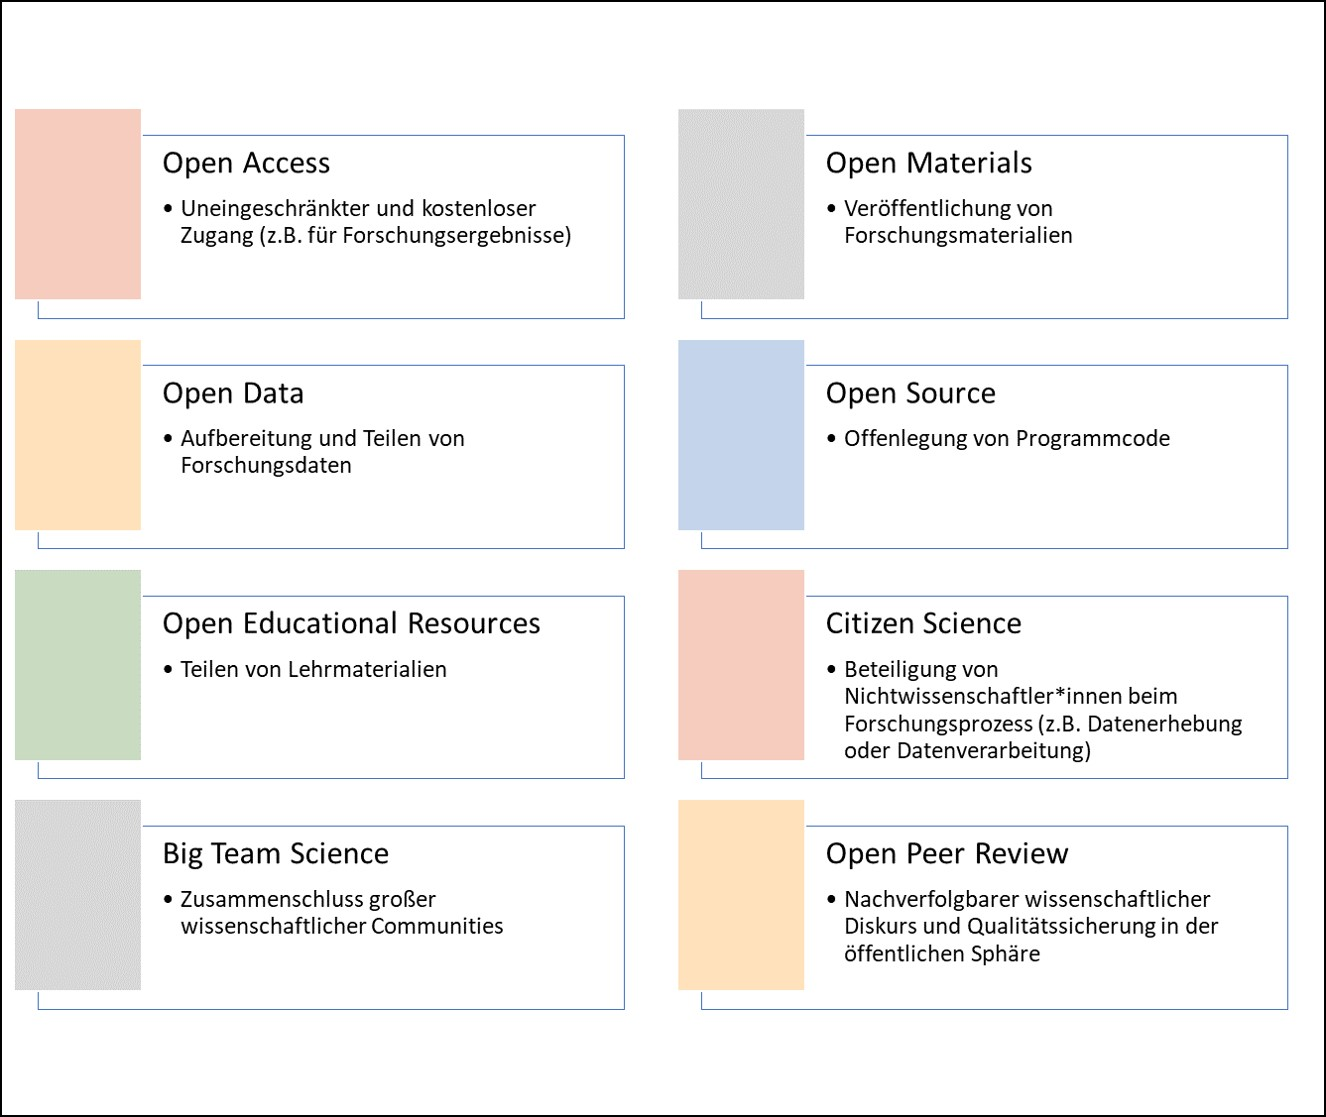
\includegraphics{images/facetten.jpg}

}

\caption{Facetten von Open Science}

\end{figure}%

\section{Literatur}\label{literatur-2}

\chapter{Wie ist mit Open Science
umzugehen?}\label{wie-ist-mit-open-science-umzugehen}

Das Thema Open Science und Replikationskrise beziehungsweise
Vertrauenskrise ist aus mehreren Gründen schwer kommunizierbar: Zuerst
einmal ist es harte Kritik an der Wissenschaft und dem
Wissenschaftssystem, die dazu missbraucht werden kann, wissenschaftliche
Befunde kleinzureden und das Vertrauen in Wissenschaft insgesamt
gefährdet. Mithilfe der hier präsentierten Argumente und Befunde lassen
sich zum Beispiel auf Wissenschaft beruhende politische oder
individuelle Entscheidungen kritisieren. Dagegen sei gesagt: Weitaus
nicht alle wissenschaftlichen Befunde sind ``falsch'' oder nicht
replizierbar. Bei vielen Punkten herrscht immer noch ein großer Konsens.

Auf der anderen Seite gehen die hier diskutierten Probleme über das
hinaus, was ganz natürlich in fast jedem wissenschaftlichen Zweig
wiederfindet. Denn je genauer man hinschaut, desto wahrscheinlicher ist
es, dass ein wissenschaftlicher Befund relativierbar ist. Widersprüche
oder Konflikte lassen sich überall finden, treten natürlicherweise auf,
und werden von Wissenschaftler*innen ins Visier genommen. Jede*r
Forschende kann berichten: Bei genauerem Hinschauen bleibt nichts
schwarz oder weiß, sondern zerfließt in viele Grautöne. Bei den im
Folgenden behandelten Replikationsfehlschlägen handelt es sich um mehr
als die wissenschaftsinhärente Ungewissheit: Sie gefährden gesamte
Wissenschaftsstränge.

Bevor wir in die Details fortschreiben, ist es außerdem wichtig
festzuhalten, dass aktuell (Herbst, 2023) die meisten der in diesem Buch
besprochenen Probleme noch nicht oder erst teilweise gelöst wurden und
auf wöchentlicher Basis heiß diskutiert werden. Nach einem Jahrzehnt der
Open Science Bewegungen ist ein Punkt erreicht, an dem die meisten
Wissenschaftler*innen ein Bewusstsein über das Problem haben. Einige
sind mit Lösungsansätzen vertraut, doch haben sich diese weder komplett
durchgesetzt, noch ist klar, welche Probleme überhaupt bereits gelöst
worden sind.

Ich verstehe Open Science als eine große Trigger-Warnung, die vor die
Sozialwissenschaften vorgeschaltet sein sollte und lautet: Achtung, wir
haben hier gerade sehr große Probleme. Es ist gut möglich, dass die
Hälfte von allem, was wir zu wissen glauben, schlichtweg falsch ist.
Meinungen über die Open Science Bewegung sind aber keineswegs homogen:
Es lässt sich hier ein Spektrum spannen zwischen ``Sollen wir wirklich
die nächsten 20 Jahre damit verbringen, herauszufinden, welche
Erkenntnisse der letzten 100 Jahre korrekt sind? Fangen wir doch einfach
nochmal bei Null an.'' und ``Eigentlich ist das ganz normal, ich sehe
keinen Grund, hier von einer `Krise' zu sprechen''.

\begin{figure}[H]

{\centering 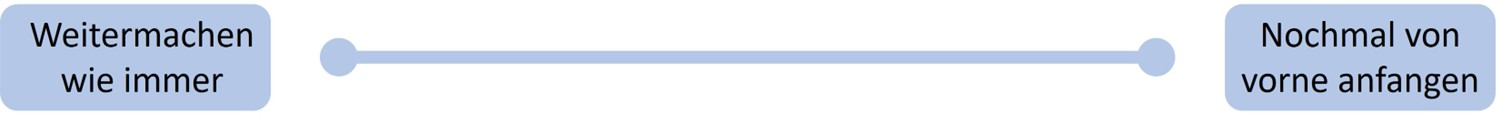
\includegraphics{images/spektrumreaktionen.jpg}

}

\caption{Spektrum der Reaktionen auf die Replikationskrise}

\end{figure}%

Besonders groß ist das Problem bei Lehrbüchern: Stellen Sie sich vor,
sie haben ein Buch über einen Teil der Psychologie (Aushängeschild ist
hier oft die Sozialpsychologie) verfasst, das auf Jahrzehnten an
Forschung besteht, hunderten Veröffentlichungen, und tausenden Studien.
Hier hilft es kaum, das Buch komplett zu ignorieren. Praktikabel, alle
Studien selbst zu replizieren, ist es allerdings auch nicht. Klar ist
den meisten Wissenschaftler*innen hierbei: So wie es bisher gelaufen
ist, kann es nicht weitergehen. Eine fünfzig prozentige Garantie für
wissenschaftliche Erkenntnisse sollte nicht der Anspruch von etwas sein,
das sich Wissenschaft nennt. Von vorne müssen wir aber auch nicht
starten.

\part{Die Geschichte der Open Science Bewegung}

Im Rahmen dieses Buches wird die Open Science Bewegung also als eine
Reaktion auf identifizierte Probleme und damit als
Selbstkorrektur-Prozess der Wissenschaft verstanden. In im Zentrum steht
ein mangelndes Vertrauen in Befunde, die in wissenschaftlichen
Fachzeitschriften veröffentlicht wurden. Einige Probleme sind schon seit
Jahrzehnten in ähnlicher Form bekannt. Bis sie allerdings öffentlich
diskutiert wurden und Lösungsvorschläge erarbeiteten, benötigte es
einschneidende Ereignisse. Aufgrund von Problemen, vergangene und für
sicher geglaubte Ergebnisse nicht \emph{replizieren} zu können (also bei
wiederholten Untersuchungen zum selben Ergebnis zu kommen) ist häufig
die Sprache von einer \emph{Replikationskrise}. Durch die Ungewissheit
über genaue Ursachen von geringen Replikationsraten wird teilweise auch
eher zu dem Begriff „Vertrauenskrise'' geraten (Feest 2019).

\section*{Vertiefende Informationen}\label{vertiefende-informationen}
\addcontentsline{toc}{section}{Vertiefende Informationen}

\markright{Vertiefende Informationen}

\begin{itemize}
\tightlist
\item
  Die Geschichte der Replikationskrise beschreiben L. D. Nelson,
  Simmons, and Simonsohn (2018) und Schimmack (2020). Eine positive
  Perspektive nehmen Korbmacher et al. (2023) ein.
\end{itemize}

\section*{Literatur}\label{literatur-3}
\addcontentsline{toc}{section}{Literatur}

\markright{Literatur}

\chapter{Anfänge einer Revolution}\label{anfuxe4nge-einer-revolution}

Um das Jahr 2010 herum häuften sich in der Psychologie Ereignisse, die
für sich genommen als Einzelfälle abgetan werden konnten, gemeinsam aber
ein negatives Bild der Wissenschaft zeichneten.

\subsection{Stapel-Affäre}\label{stapel-affuxe4re}

Durch einen Zufall entdeckten Nachwuchswissenschaftler im Jahr 2011,
dass die Daten einer Studie ihres Kollegen, Diederik Stapel, von
niemandem jemals erhoben wurden. Sie waren ausgedacht, bzw. fabriziert.
Stand Juli 2024 wurden 58 von Stapels Fachartikel identifiziert und
zurückgezogen, deren Daten fabriziert oder geschönt wurden.\footnote{Mittels
  der Retraction Database lassen sich nach Thema, Autor*in, Zeitschrift,
  usw. zurückgezogene Artikel durchsuchen:
  http://retractiondatabase.org/} Wissenschaftliche Institutionen wie
der Begutachtungsprozess von Artikeln durch Fachkolleg*inen, deren Zweck
die Qualitätssicherung war, hatten versagt. Seit dem Vorfall sind einige
weitere Fälle bekannt geworden, teilweise durch erneute Analyse von
Daten der jeweiligen Studien (O'Grady 2021) und oft durch Whistleblower,
also durch Personen, die zu ihrem Schutz anonym bleiben wollen. Umfragen
in den Niederlanden unter Forschenden haben ergeben, dass Fälschung oder
Schönigung von Daten von bis zu 10\% aller Personen durchgeführt wird
(Gopalakrishna, Riet, et al. 2021). Dabei ist zu beachten, dass Studien
durch gefälschte Daten besonders innovativ, überraschend, oder klar
werden - Eigenschaften, die die Veröffentlichung in einer
Fachzeitschrift wahrscheinlicher machen.

\subsection{Bem: Die Zukunft
erfühlen}\label{bem-die-zukunft-erfuxfchlen}

Kurze Zeit später veröffentliche Daryl Bem, bekannt durch grundlegende
psychologisch-philosophische Theorien wie der Self-Perception-Theory
(Bem 1967), den Befund, dass Personen die Zukunft vorhersagen können
(Bem 2011). Genauer gesagt, können manche Personen unter bestimmten
Dingen, die Zukunft vorhersagen. In 8 Studien fand die
Forschendengruppe, dass Personen Vorhersagen über erotische Bilder
machen konnten. Die Ergebnisse wurden in der hoch angesehenen
Fachzeitschrift \emph{Journal of Personality and Social Psychology}
veröffentlicht. Vielen Psycholog*innen war sofort klar: Entweder,
Grundlegende Annahmen ihres Weltbildes waren falsch (``Personen können
nicht die Zukunft vorhersagen'') oder es stimmte etwas mit den
Ergebnissen nicht. Mehrere Forschende versuchten sich daran, zu
erklären, wie es zu den Ergebnissen kam. Analysen mit alternativen
statistischen Methoden führten zur selben Schlussfolgerung (Wagenmakers
et al. 2011), Replikationen durch unabhängige Forschende schlugen jedoch
fehl Roe, Grierson, and Lomas (2012).

\subsection{\texorpdfstring{Bargh: Beeinflussen durch
\emph{Priming}}{Bargh: Beeinflussen durch Priming}}\label{bargh-beeinflussen-durch-priming}

Seine Studien wurden im Marketing gefeiert und als
Neurowissenschaftliche Erkenntnisse verkauft: Wer ein heißes Getränk (im
Vergleich zu einem kalten) trinkt, schätzt andere Personen als
``wärmer'' (großzügig, rücksichtsvoll) ein (Williams and Bargh 2008).
Wer Anagramme löst, die etwas mit hohem Alter zu tun haben (z.B.
PFLEGEHEIM, GRAU, oder zum selbst probieren GHOSTECK), geht danach in
langsamerem Tempo (Bargh, Chen, and Burrows 1996). Viele dieser Studien
wurden repliziert: Forschenden fiel in der Anagramme-Studie auf, dass
Bargh und Kolleg*innen die Zeit mit Stoppuhren gemessen hatten und dabei
wussten, welche Person die ``Alt''-Wörter und welche die neutralen
Anagramme gelöst hatten - dabei lernt jede*r Psychologie-Studierende im
ersten Jahr, dass das nicht der Fall sein sollten und
Versuchsleiter*innen ``blind'' gegenüber dem Untersuchungszweck und der
Zuordnung der Personen zu den Gruppen sein sollte. In ihrer Replikation
(Doyen et al. 2012) ließen Doyen und Kolleg*innen die Zeit mit
Lichtschranken erfassen und maßen selbst wie Bargh et al.~in der
Originalstudie. Bei der problematischen Messung kam dasselbe raus, die
Lichtschranken, denen vorher nicht verraten wurde, welche Hypothese mit
ihnen untersucht werden sollten und welche Personen welche Anagramme
lösen mussten, konnten den Effekt jedoch nicht replizieren.

\subsection{Literatur}\label{literatur-4}

\chapter{Bestandsaufnahme}\label{bestandsaufnahme}

Eine ähnliche Vertrauenskrise gab es in der Sozialpsychologie in den
1960er Jahren (Daniel Lakens 2023). Ein entscheidender Unterschied war
diesmal die Bestandsaufnahme: Parallel zu diesen eigenartigen Befunden
oder \emph{Anomalien} vernetzten sich Psycholog*innen um Brian Nosek
international und untersuchten die Replizierbarkeit von 100 Studien aus
namhaften psychologischen Fachzeitschriften (Open Science Collaboration
2015). Sie fanden heraus, dass sich nur 39 der 100 Originalbefunde
replizieren ließen. Bei allen anderen Studien, waren die
Replikationsergebnisse anders als die ursprünglichen Ergebnisse. Viele
weitere Großprojekte folgten, alle mit ähnlichen Ergebnissen: Die
Replikationsraten lagen weit unter den Gewünschten.

\begin{tcolorbox}[enhanced jigsaw, title=\textcolor{quarto-callout-note-color}{\faInfo}\hspace{0.5em}{Kritische Betrachtung der Open Science Collaboration, 2015}, colbacktitle=quarto-callout-note-color!10!white, rightrule=.15mm, titlerule=0mm, left=2mm, bottomrule=.15mm, arc=.35mm, leftrule=.75mm, toprule=.15mm, opacityback=0, breakable, bottomtitle=1mm, colframe=quarto-callout-note-color-frame, toptitle=1mm, opacitybacktitle=0.6, coltitle=black, colback=white]

Obgleich dieses „Reproducibility Project Psychology'' die gesamte
Fachgemeinschaft zutiefst erschütterte und den Weg für einen
Paradigmenwechsel ebnete, bemängeln manche Forschende auch negative
Auswirkungen auf nachfolgende Replikationsforschung. Indem 100 Studien
gleichzeitig von einer Gruppe aus über 100 Forschenden veröffentlicht
wurden, setzte das Projekt unrealistische Maßstäbe für
Replikationsforschung. Gleichzeitig war die Qualitätskontrolle dabei
weniger streng, da die einzelnen Studien nicht alle in dem Maße
begutachtet werden konnten, wie es bei einer traditionellen
Veröffentlichung der Fall gewesen wäre (z.B. Röseler et al. (2022)).
Einige gleichermaßen ambitionierte Vorhaben wurden veröffentlicht, wie
zum Beispiel die ManyLabs Studien (z.B. Klein et al. (2014); Klein et
al. (2018)) oder Versuche, bei denen unabhängige Gruppen dieselben
Hypothesen testeten und replizierten (Landy et al. 2020). Oft
beschränken sich diese Vorhaben auf Studien, die sich im Rahmen einer
Online-Befragung replizieren lassen. Formate wie Längsschnittstudien
oder Verhaltensbeobachtungen sind dabei unterrepräsentiert.

\end{tcolorbox}

Zahlreiche Verbünde folgten. Einige Projekte konzentrierten sich auf
einzelne Phänomene. Beispielsweise haben sich 17 Forschungsgruppen
zusammengetan, um den Befund des \emph{Facial Feedback} (Strack, Martin,
and Stepper 1988) zu replizieren (Wagenmakers et al. 2016). Dabei geht
darum, dass Personen einen Stift mit den Zähnen festhalten und dabei je
nach Ausrichtung des Stiftes entweder diejenigen Muskeln anspannen, die
sie auch zum Lachen benötigen oder eben nicht. In der
``Lachen''-Bedingung fanden die Versuchspersonen im Anschluss Comics
witziger. Die Replikation schlug fehl. 2022 wurde eine weitere Studie
mit über 3000 Versuchspersonen aus 19 Ländern veröffentlicht - diesmal
auch mit direkter Beteiligung von Fritz Strack, der die Originalstudie
durchgeführt hatte (Coles et al. 2022). Wieder zeigte sich, dass die
Position eines Stiftes im Mund sich nicht auf die Bewertung von Stimuli
auswirkt. Jenseits von sozialpsychologischen Befunden konzentrierten
sich Forschende auch auf Bereiche wie Forschung mit Babys
(Byers-Heinlein et al. 2020) oder auf ganze Zeitschriften (Camerer et
al. 2018).

\textbf{Liste großer Replikationsprojekte (siehe auch
\href{https://forrt.org/replication-hub/}{FORRT Replication Hub})}

\begin{longtable}[]{@{}
  >{\raggedright\arraybackslash}p{(\columnwidth - 4\tabcolsep) * \real{0.1979}}
  >{\raggedright\arraybackslash}p{(\columnwidth - 4\tabcolsep) * \real{0.2620}}
  >{\raggedright\arraybackslash}p{(\columnwidth - 4\tabcolsep) * \real{0.5401}}@{}}
\toprule\noalign{}
\endhead
\bottomrule\noalign{}
\endlastfoot
\textbf{Projekt} & \textbf{Thema} & \textbf{Link} \\
Reproducibility Project: Psychology & Psychologie &
\url{https://osf.io/ezcuj/} \\
CORE & Entscheidungsforschung & \url{https://osf.io/5z4a8/} \\
Data Replicada & Konsumentenverhalten und Entscheidungsforschung &
\url{https://datacolada.org/archives/category/replication} \\
Many Labs 1 & Psychologie & \url{https://osf.io/wx7ck/} \\
Many Labs 2 & Psychologie & \url{https://osf.io/8cd4r/} \\
Many Labs 3 & Psychologie & \url{https://osf.io/ct89g/} \\
Many Labs 4 & Psychologie & \url{https://osf.io/8ccnw/} \\
Many Labs 5 & Psychologie & \url{https://osf.io/7a6rd/} \\
Soto & Persönlichkeitspsychologie &
\url{https://doi.org/10.1177/0956797619831612} \\
Social Sciences Replication Project & Verhaltensforschung &
\href{http://www.socialsciencesreplicationproject.com/}{http://www.socialsciencesreplicationproject.com} \\
Registered Replication Reports & Verschiedene & -- \\
Many Babies 1 & Entwicklungspsychologie &
\href{https://manybabies.org/}{https://manybabies.org} \\
Sports Sciences Replications & Sportwissenschaften &
\href{https://ssreplicationcentre.com/}{https://ssreplicationcentre.com} \\
Hagen Cumulative Science Project & Psychologie &
\url{https://osf.io/d7za8/} \\
I4R Replications & Politikwissenschaften &
\url{https://i4replication.org/reports.html} \\
Experimental Philosophy & Experimentelle Philosophie &
h\href{https://doi.org/10.1007/s13164-018-0400-9}{ttps://doi.org/10.1007/s13164-018-0400-9} \\
Reproducibility Project: Cancer & Krebsforschung (Medizin) &
\url{https://www.cos.io/rpcb} \\
SCORE & Sozialwissenschaften & \url{https://www.cos.io/score} \\
REPEAT & Gesundheitssystem &
\href{https://www.repeatinitiative.org/}{https://www.repeatinitiative.org} \\
CREP & Psychologie &
\href{https://www.crep-psych.org/}{https://www.crep-psych.org} \\
Boyce et al., 2023 & Psychologie &
\url{https://doi.org/10.1098/rsos.231240} \\
ReproSci & Biologie &
\href{https://reprosci.epfl.ch/}{https://reprosci.epfl.ch} \\
Boyce et al.~2024 & Psychologie &
\url{https://doi.org/10.31234/osf.io/an3yb} \\
\end{longtable}

\subsection{Definition von
Replizierbarkeit}\label{definition-von-replizierbarkeit}

Zu sagen, was repliziert werden konnte und was nicht, ist erst nach
einer Definition möglich. Im Sprachgebrauch von Forschenden wird mit
„wurde repliziert'' gemeint, dass ein Replikationsversuch zu gleichen
Ergebnissen wie eine Originalstudie gekommen ist. Zu
Replikationsfehlschläge wird „konnte nicht repliziert werden'' gesagt,
subtil davon abweichend kann „wurde nicht repliziert'' meinen, dass
keine Replikationsversuche existieren oder sie fehlschlugen. Für eine
Wissenschaft, die über 100 Jahre alt ist, scheint es überraschend, dass
noch immer keine klare Definition wichtiger Konzepte rund um das Thema
Replikation vorliegt, geschweige denn es zur Routine gehört, Studien zu
replizieren. Während sich in verschiedenen Feldern abweichende
Taxonomien durchgesetzt haben, sieht die Verwendung in diesem Buch wie
in der Tabelle beschrieben aus.

\begin{longtable}[]{@{}llll@{}}
\caption{Replikations-Taxonomie nach Turing Way (The Turing Way
Community and Scriberia 2024)}\tabularnewline
\toprule\noalign{}
& & Daten & \\
\midrule\noalign{}
\endfirsthead
\toprule\noalign{}
& & Daten & \\
\midrule\noalign{}
\endhead
\bottomrule\noalign{}
\endlastfoot
& & gleich & unterschiedlich \\
\textbf{Analyse} & gleich & reproduzierbar & replizierbar \\
& unterschiedlich & robust & verallgemeinerbar \\
\end{longtable}

\subsection{Weiterführende Literatur}\label{weiterfuxfchrende-literatur}

Für eine systematischere, in den Informationswissenschaften verankerte
Taxonomie zur Art der Replikation siehe (Plesser 2018). Eine an den
statistischen Methoden angelehnte Taxonomie für die Ergebnisse von
Replikationsstudien haben LeBel et al. (LeBel et al. 2019)
vorgeschlagen. Philosophisch diskutiert wird Replikationsnähe zum
Beispiel von (Choi 2023) und (Leonelli 2023).

\begin{longtable}[]{@{}
  >{\raggedright\arraybackslash}p{(\columnwidth - 2\tabcolsep) * \real{0.5628}}
  >{\raggedright\arraybackslash}p{(\columnwidth - 2\tabcolsep) * \real{0.4372}}@{}}
\caption{Replikationstaxonomie}\tabularnewline
\toprule\noalign{}
\begin{minipage}[b]{\linewidth}\raggedright
\textbf{Unterscheidungskriterium}
\end{minipage} & \begin{minipage}[b]{\linewidth}\raggedright
\textbf{Ausprägungen}
\end{minipage} \\
\midrule\noalign{}
\endfirsthead
\toprule\noalign{}
\begin{minipage}[b]{\linewidth}\raggedright
\textbf{Unterscheidungskriterium}
\end{minipage} & \begin{minipage}[b]{\linewidth}\raggedright
\textbf{Ausprägungen}
\end{minipage} \\
\midrule\noalign{}
\endhead
\bottomrule\noalign{}
\endlastfoot
Ergebnisse einer Replikationsstudie & Erfolgreich

Fehlgeschlagen

Unklar oder gemischt \\
Nähe einer Replikationsstudie zur Originalstudie (in Anlehnung an Lebel
REF und Hüffmeier et al REF) &
\begin{minipage}[t]{\linewidth}\raggedright
\textbf{Direkte Replikation}\\
(selbe Versuchsleiter*innen,\\
selbe Versuchsmaterialien,\\
neue Versuchspersonen)

\textbf{Nahe Replikation}\\
(andere Versuchsleiter*innen,\\
möglichst ähnliche Versuchsmaterialien,\\
neue Versuchspersonen)

\textbf{Konzeptuelle oder konstruktive Replikation}\\
(andere Versuchsleiter*innen,\\
andere Versuchsmaterialien,\\
neue Versuchspersonen)\strut
\end{minipage} \\
Ziel der Replikation & \begin{minipage}[t]{\linewidth}\raggedright
\textbf{Reproduktion}\\
Mit selben Daten und selbem Programmiercode zu denselben Ergebnissen
gelangen

\textbf{Replikation}\\
Mit anderen Daten zu denselben Ergebnissen gelangen\strut
\end{minipage} \\
\end{longtable}

\subsection{„Eine Schwalbe macht noch keinen
Sommer''}\label{eine-schwalbe-macht-noch-keinen-sommer}

Ob an einem wissenschaftlichen Befund „etwas dran ist'', er also einen
Wahrheitsanspruch hat, hängt -- neben seiner eigentlichen Art der
Etablierung -- bei der Replikationsforschung von vielen Faktoren ab. Was
waren die Ergebnisse der Replikationsstudie? Wie viele und wie
unterschiedliche Studien wurden durchgeführt? Wie sahen die genauen
Methoden aus? Was waren die Unterschiede zwischen Replikationen und
Originalstudie? Während Einzelstudien immer einen Erkenntnisgewinn
liefern (mindestens, ob eine bestimmte Methode praktikabel ist,
(Sikorski and Andreoletti 2023), können sie je nach Forschungsgebiet
stark variieren Landy et al. (2020). Für das Gesamtbild braucht es mehr,
wie zum Beispiel eine statistische Aggregation aller Einzelbefunde im
Rahmen einer Meta-Analyse. Ein Beispiel mit Fantasiedaten befindet sich
dazu in der folgenden Abbildung.

Betrachtet man viele Studien, die den Zusammenhang zweier Dinge, wie zum
Beispiel Einkommen und Bildungsabschluss, untersucht haben, so werden
sich die Studien hinsichtlich der Details unterscheiden: Was wurde alles
zum Einkommen gezählt (Netto, Brutto, Sozialleistungen, Einkommen von
Familienangehörigen, Werte über einen Zeitraum oder von einem bestimmten
Zeitpunkt aus der Vergangenheit, usw.) oder auch welche Personen befragt
wurden (Studierende, Berufstätige, wurden Befragte bezahlt, usw.). Alle
diese Unterschiede wirken sich möglicherweise auf den Zusammenhang aus,
und selbst wenn sie es nicht tun, unterliegen Zusammenhänge oft
Schwankungen, die sich durch die Messmethoden ergeben. In dem Beispiel
lässt sich die Stärke des Zusammenhangs auf eine Zahl und eine
dazugehörige Präzision herunterbrechen. Die Zahl heißt hier
``Korrelation'' und die Schärfe ``Fehlerbalken''. In dem Wald-Diagramm
(\emph{Forest Plot / Blobbogram}) sind mögliche Korrelationen aus
verschiedenen Studien abgebildet. Im Rahmen einer Meta-Analyse können
Studienergebnisse anschließend kombiniert und Unterschiede untersucht
werden.

\begin{Shaded}
\begin{Highlighting}[]
\FunctionTok{library}\NormalTok{(ggplot2)}
\FunctionTok{library}\NormalTok{(metafor)}
\end{Highlighting}
\end{Shaded}

\begin{verbatim}
Lade nötiges Paket: Matrix
\end{verbatim}

\begin{verbatim}
Lade nötiges Paket: metadat
\end{verbatim}

\begin{verbatim}
Lade nötiges Paket: numDeriv
\end{verbatim}

\begin{verbatim}

Loading the 'metafor' package (version 4.6-0). For an
introduction to the package please type: help(metafor)
\end{verbatim}

\begin{Shaded}
\begin{Highlighting}[]
\FunctionTok{set.seed}\NormalTok{(}\DecValTok{10}\NormalTok{)}
\NormalTok{k }\OtherTok{\textless{}{-}} \DecValTok{15}
\NormalTok{cors }\OtherTok{\textless{}{-}} \FunctionTok{data.frame}\NormalTok{(}\StringTok{"Stichprobenumfang"} \OtherTok{=} \FunctionTok{round}\NormalTok{(}\FunctionTok{rchisq}\NormalTok{(}\AttributeTok{n =}\NormalTok{ k, }\AttributeTok{df =} \DecValTok{2}\NormalTok{, }\AttributeTok{ncp =} \DecValTok{0}\NormalTok{)}\SpecialCharTok{*}\DecValTok{5}\SpecialCharTok{+}\DecValTok{10}\NormalTok{, }\AttributeTok{digits =} \DecValTok{0}\NormalTok{)}
\NormalTok{                   , }\StringTok{"Korrelation"} \OtherTok{=} \FunctionTok{rnorm}\NormalTok{(}\AttributeTok{n =}\NormalTok{ k, }\AttributeTok{mean =}\NormalTok{ .}\DecValTok{05}\NormalTok{, }\AttributeTok{sd =}\NormalTok{ .}\DecValTok{3}\NormalTok{)}
\NormalTok{                   , }\StringTok{"Studie"} \OtherTok{=} \FunctionTok{paste}\NormalTok{(}\StringTok{"Studie"}\NormalTok{, }\FunctionTok{toupper}\NormalTok{(letters[}\DecValTok{1}\SpecialCharTok{:}\NormalTok{k]), }\AttributeTok{sep =} \StringTok{" "}\NormalTok{)}
\NormalTok{                   , }\StringTok{"yi"} \OtherTok{=} \ConstantTok{NA}
\NormalTok{                   , }\StringTok{"vi"} \OtherTok{=} \ConstantTok{NA}
\NormalTok{                   )}

\NormalTok{cors[, }\DecValTok{4}\SpecialCharTok{:}\DecValTok{5}\NormalTok{] }\OtherTok{\textless{}{-}}\NormalTok{ metafor}\SpecialCharTok{::}\FunctionTok{escalc}\NormalTok{(}\AttributeTok{ni =}\NormalTok{ cors}\SpecialCharTok{$}\NormalTok{Stichprobenumfang, }\AttributeTok{ri =}\NormalTok{ cors}\SpecialCharTok{$}\NormalTok{Korrelation, }\AttributeTok{measure =} \StringTok{"COR"}\NormalTok{)}
\NormalTok{cors}\SpecialCharTok{$}\NormalTok{ucb }\OtherTok{\textless{}{-}}\NormalTok{ cors}\SpecialCharTok{$}\NormalTok{yi }\SpecialCharTok{+} \FunctionTok{qnorm}\NormalTok{(.}\DecValTok{975}\NormalTok{)}\SpecialCharTok{*}\NormalTok{cors}\SpecialCharTok{$}\NormalTok{vi}
\NormalTok{cors}\SpecialCharTok{$}\NormalTok{lcb }\OtherTok{\textless{}{-}}\NormalTok{ cors}\SpecialCharTok{$}\NormalTok{yi }\SpecialCharTok{{-}} \FunctionTok{qnorm}\NormalTok{(.}\DecValTok{975}\NormalTok{)}\SpecialCharTok{*}\NormalTok{cors}\SpecialCharTok{$}\NormalTok{vi}



\FunctionTok{ggplot}\NormalTok{(cors, }\FunctionTok{aes}\NormalTok{(}\AttributeTok{x =}\NormalTok{ Korrelation, }\AttributeTok{y =} \FunctionTok{reorder}\NormalTok{(Studie, Korrelation))) }\SpecialCharTok{+} 
  \FunctionTok{geom\_point}\NormalTok{() }\SpecialCharTok{+} \FunctionTok{geom\_errorbar}\NormalTok{(}\AttributeTok{xmin =}\NormalTok{ cors}\SpecialCharTok{$}\NormalTok{lcb, }\AttributeTok{xmax =}\NormalTok{ cors}\SpecialCharTok{$}\NormalTok{ucb) }\SpecialCharTok{+} 
  \FunctionTok{geom\_vline}\NormalTok{(}\AttributeTok{xintercept =} \DecValTok{0}\NormalTok{, }\AttributeTok{lty =} \DecValTok{2}\NormalTok{) }\SpecialCharTok{+} \FunctionTok{theme\_classic}\NormalTok{() }\SpecialCharTok{+} \FunctionTok{ylab}\NormalTok{(}\StringTok{""}\NormalTok{) }\SpecialCharTok{+} 
  \FunctionTok{xlim}\NormalTok{(}\FunctionTok{c}\NormalTok{(}\SpecialCharTok{{-}}\NormalTok{.}\DecValTok{4}\NormalTok{, .}\DecValTok{6}\NormalTok{))}
\end{Highlighting}
\end{Shaded}

\includegraphics{bestandsaufnahme_files/figure-pdf/unnamed-chunk-1-1.pdf}

\subsection{Phänomen-zentrierte
Replikationsprojekte}\label{phuxe4nomen-zentrierte-replikationsprojekte}

Im Gegensatz zu dem breit gefächerten RPP und anderen Versuchen, die
Replikationsrate zu schätzen, haben sich andere Versuche auf
grundlegende Phänomene fokussiert. Dutzende Gruppen auf der ganzen Welt
haben sich in solchen Fällen zusammengeschlossen, auf einen
Versuchsaufbau geeinigt, und führen die Studien mit einer enormen Anzahl
an Versuchspersonen durch. Die meisten dieser Vorhaben stammen aus der
Psychologie. Während die dabei gefundenen Effektstärken, also sozusagen
die Deutlichkeit eines Zusammenhanges oder Befundes, in fast allen
Fällen weit unter denen bisheriger Studien lagen (Kvarven, Strømland,
and Johannesson 2020), waren sie zudem beim Großteil der Studien null,
die Phänomene waren also „nicht sichtbar'' (Alogna et al. 2014; Eerland
et al. 2016; Bouwmeester et al. 2017; O'Donnell et al. 2018; Wagenmakers
et al. 2016.; Cheung et al. 2016; Vaidis et al. 2024; Rife et al. 2024).
So konnte beispielsweise mit einer enormen Präzision gezeigt werden,
dass eine Geschichte über einen Professor Versuchspersonen in einem
anschließenden Leistungstest *nicht* schlauer macht (O'Donnell et al.
2018).

\begin{tcolorbox}[enhanced jigsaw, title=\textcolor{quarto-callout-note-color}{\faInfo}\hspace{0.5em}{Effiziente Nutzung von Ressourcen?}, colbacktitle=quarto-callout-note-color!10!white, rightrule=.15mm, titlerule=0mm, left=2mm, bottomrule=.15mm, arc=.35mm, leftrule=.75mm, toprule=.15mm, opacityback=0, breakable, bottomtitle=1mm, colframe=quarto-callout-note-color-frame, toptitle=1mm, opacitybacktitle=0.6, coltitle=black, colback=white]

Wie geht man mit Ressourcen bei Replikationen um? Bei Zusammenschlüssen
vieler Forschender stellt sich diese Frage unweigerlich. Erstellen alle
Gruppen unabhängig voneinander die Studie? Halten sich alle an ein zuvor
abgestimmtes Protokoll? Führen sie die Studie nacheinander durch um
voneinander zu lernen? Bei \emph{Registered Replication Reports} wird
für gewöhnlich von einem zuvor mit anderen Forschenden (z.B. den
Autor*innen der Originalstudie) ein Versuchsaufbau abgestimmt. In
anderen Fällen wird gemeinsam ein Versuchsaufbau erarbeitet, der zum
Testen der Theorie ideal sein sollte (\emph{Creative Destruction
Approach}, Tierney et al. (2020)). Teams in verschiedenen Ländern
übersetzen das Protokoll dann und halten sich bei der Durchführung eng
daran. Diese Protokolle sind manchmal nicht im Vorhinein getestet
(Buttliere 2024), basieren oft aber auf erfolgreichen, namhaften
Studien. Das hat den Vorteil, dass Unterschiede zwischen den Gruppen
nicht auf Unterschiede in der Durchführung zurückzuführen sind und sich
Kulturen vergleichen lassen (Kakinohana, Pilati, and Klein 2022). Ein
Nachteil dabei ist jedoch, dass, wenn an einem, zwei, oder fünf
Standorten das Experiment schon nicht funktioniert, es fraglich ist, ob
die übrigen 30 Gruppen es auch probieren sollten. In den Worten von
Buttliere (2024): ``Wer bekommt bessere Ergebnisse? 39 Personen, die
etwas zum ersten Mal tun, oder eine Person, die etwas 39 Mal tut?''

\end{tcolorbox}

\subsection{Disziplin-zentrierte
Replikationsprojekte}\label{disziplin-zentrierte-replikationsprojekte}

Ungefähr die Hälfte aller psychologischen Befunde ist also nicht
replizierbar. Heißt das, alle Sozialwissenschaftlichen Lehrbücher aus
allen Disziplinen sind zur Hälfte falsch? Die klare Antwort heißt
\emph{nein}. Die akkurate Antwort lautet \emph{kommt darauf an}.

\subsubsection{Jenseits der Psychologie}\label{jenseits-der-psychologie}

Inwiefern es auf die Disziplin innerhalb der Sozialwissenschaften
ankommt wurde bisher vor allem in der Psychologie untersucht. Aktuelle
Tendenzen weisen darauf hin, dass Replikationsraten in der
Persönlichkeitspsychologie und kognitiven Psychologie (Soto 2019) höher
liegen als die in der Sozialpsychologie (Open Science Collaboration
2015) oder im Marketing (Charlton 2022). Während schon hunderte
Replikationsversuche für sozialpsychologische Studien veröffentlicht
sind, sind es in anderen Bereichen wie dem Marketing aktuell weniger -
Stand Oktober 2022 sogar nur 9. Bereiche außerhalb der Psychologie sind
von Replikationsproblemen ebenfalls betroffen. Von Problemen der
Replizierbarkeit, Reproduzierbarkeit, und Nachvollziehbarkeit sind fast
alle Disziplinen betroffen. Neue Lösungsansätze werden in Medizin,
Biologie, Chemie, Physik, Geschichtswissenschaften,
Politikwissenschaften, Erziehungswissenschaften, Informatik, und vielen
weiteren Bereichen diskutiert.

\subsection*{Literatur}\label{literatur-5}
\addcontentsline{toc}{subsection}{Literatur}

\chapter{Wandel im System}\label{wandel-im-system}

Seit dem Bekanntwerden der geringen Replizierbarkeit psychologischer
Studien wurde das wissenschaftliche System in vielen Aspekten
hinsichtlich seiner Offenheit und Transparenz verändert. Einige
Zeitschriften setzen für die Veröffentlichung wissenschaftlicher Artikel
voraus, dass die Daten öffentlich zugänglich sind beziehungsweise
erklärt ist, weshalb das nicht der Fall ist (z.B. bei Daten, die sich
schwierig anonymisieren lassen). In seltenen Fällen wie bei der
Zeitschrift Meta-Psychology rechnen Wissenschaftler*innen alle
Ergebnisse nach. Als Antithese zum ``Impact Factor'', einer Kennzahl,
die angibt wie oft eine Zeitschrift zitiert wird und nachweislich nichts
mit der Qualität der darin enthaltenen Forschung zu tun hat (Brembs
2018), wurde der TOP-Factor eingeführt (TOP: Transparency and Openness
Promotion). Dieser gibt für eine Liste von Kriterien an, in welchem Maße
sie von verschiedenen Zeitschriften erfüllt werden. In anderen Feldern
wie Betriebswirtschaftslehre oder Marketing werden Zeitschriften sogar
von wenigen ausgewählten Forschenden über Ratingskalen bewertet, die
jährlich als Rankings veröffentlicht werden. TOP-Factors hingegen sind
objektiv, werden stetig aktualisiert, und sind unter topfactor.org
öffentlich einsehbar und nachvollziehbar. Für jeden Faktor gibt es vier
Stufen: Keine erwähnung, Level 1, Level 2, und Level 3. Level 3 ist
dabei das Ideal, zum Beispiel hieße das im Hinblick auf Transparenz von
Daten, dass ein Artikel erst dann veröffentlicht wird, wenn die Daten
öffentlich verfügbar sind und die Analysen von einer unabhängigen Person
erfolgreich nachgerechnet (\emph{reproduziert}) wurden. Zum Scoring
einer Zeitschrift werden für die Levels 1-3 entsprechende Punkte
vergeben und aufsummiert.\footnote{Sozialwissenschaftler*innen wissen,
  dass das Aufsummieren der Werte unsinnig ist, da Level 2 nicht
  ``doppelt so gut'' wie Level 1 ist, und die verschiedenen Faktoren
  nicht immer gleich gewichtet werden sollten - rechnerisch wird aber
  genau das angenommen. Als heuristische Schätzung der Offenheit von
  Zeitschriften ist dieses Vorgehen jedenfalls sinnvoller als
  bibliometrische Maße.}

\begin{longtable}[]{@{}
  >{\raggedright\arraybackslash}p{(\columnwidth - 2\tabcolsep) * \real{0.1381}}
  >{\raggedright\arraybackslash}p{(\columnwidth - 2\tabcolsep) * \real{0.8619}}@{}}
\caption{Übersicht über TOP Richtlinien}\tabularnewline
\toprule\noalign{}
\begin{minipage}[b]{\linewidth}\raggedright
Faktor
\end{minipage} & \begin{minipage}[b]{\linewidth}\raggedright
Erklärung
\end{minipage} \\
\midrule\noalign{}
\endfirsthead
\toprule\noalign{}
\begin{minipage}[b]{\linewidth}\raggedright
Faktor
\end{minipage} & \begin{minipage}[b]{\linewidth}\raggedright
Erklärung
\end{minipage} \\
\midrule\noalign{}
\endhead
\bottomrule\noalign{}
\endlastfoot
Zitation von Daten & Den meisten Forschungsartikeln liegen Daten
zugrunde. Spezifisch geht es hier um die Möglichkeit, Daten unabhängig
von den Artikeln zitieren zu können (z.B. über eine eigene Kennung, wie
ein \emph{Digital Object Identifier} {[}DOI{]}). \\
Transparenz von Daten & Wenn möglich sollten Daten veröffentlicht
werden. Das ist direkt über Fachzeitschriften oder über sogenannte
\emph{Forschungsdaten-Repositorien} möglich. \\
Transparenz vom Analyse-Code & Mit dem Analyse-Code werden die
Forschungsdaten ausgewertet. Andere Forschende sollten die Möglichkeit
haben, den Code auszuführen und die Ergebnisse zu \emph{reproduzieren}
bzw. zu prüfen. \\
Transparenz der Forschungsmaterialien & Bei Forschungsmaterialien kann
es sich um Fragebögen, gezeigte Bilder oder Filme, aber auch
präsentierte Gerüche, verkostete Früchte, oder Programme handeln. Wenn
möglich, sollten auch sie (in digitaler Form) in einem Repositorium
abgelegt werden. Das ist bei Gegenständen selbstverständlich nicht
möglich. Bei Genen gibt es beispielsweise \emph{alphanumerische Codes},
mittels welchen sich Forschende verständigen. \\
Richtlinien zum Beschreiben des Versuchsaufbaus und der Analysen & Zum
Verständnis aber auch zur Nachbildung einer Studie ist es wichtig, den
Versuchsaufbau genau zu beschreiben. Einige Zeitschriften haben in den
letzten Jahren beispielsweise die Wortbegrenzung für die entsprechende
Abschnitte in Forschungsartikeln aufgehoben. \\
Präregistrierung von Studien & Siehe auch Abschnitt zu
Präregistrierungen in diesem Buch: Sofern eine Studie Hypothesen testet
(also z.B. Erwartungen oder Vorhersagen für das Ergebnis), sollten diese
im Vorhinein festgelegt sein und nach dem Sehen der Ergebnisse nicht an
diese angepasst werden. Idealerweise fordern Fachzeitschriften für
solche Studien Präregistrierungen und verpflichten Forschende den Link
zu ihnen anzugeben. \\
Präregistrierung des Analyseplans & Der Weg von den Daten zu den
Ergebnissen ist ein langer. Die Ergebnisse hängen von vielen
Entscheidungen ab. Um sich dieser Flexibilität zu berauben, sollten
Forschende den Analyseplan in der Präregistrierung beschreiben. \\
Replikation & Trotz ihres Wertes gibt es noch immer viele Zeitschriften,
die keine Replikationsstudien veröffentlichen. Im Mindestfall ermutigen
Zeitschriften Forschende dazu, Replikationsstudien bei ihnen
einzureichen. \\
\end{longtable}

Am Wandel beteiligt sind vor allem Jungwissenschaftler*innen oder
Forschende im frühen Karrierestadium (\emph{Early Career Researchers},
ECR). An vielen Universitäten haben sich in den letzten Jahren Open
Science Initiativen oder regelmäßige Treffen („Reproducibili-Tea'')
herausgebildet, die fast ausschließlich aus ``Post Docs'' (Personen nach
der Promotion ohne Professur), Promovierenden (Doktoranden), und
Studierenden bestehen. In Deutschland haben sie sich zum NOSI (Netzwerk
der Open Science Initiativen Deutschland) vernetzt (Schönbrodt, Baumert,
et al. 2022).

\subsection{Hat sich die Replizierbarkeitsrate
erhöht?}\label{hat-sich-die-replizierbarkeitsrate-erhuxf6ht}

Die Replikationskrise dauert nun schon über ein Jahrzehnt an und einiges
hat sich geändert. Ist dadurch auch das Problem der Replizierbarkeit
gelöst? Zum einen ist für viele Bereiche noch gar nicht klar, was sich
replizieren lässt. Im Marketing führte die Zeitschrift \emph{Journal of
Business Research} kurzzeitig eine Replikationsecke ein (Easley and
Madden 2013), welche dann jedoch in eine andere Zeitschrift verlagert
wurde. Aktuell sind Projekte in Arbeit, die die Replizierbarkeit für
verschiedene Disziplinen schätzen. Deren Ergebnisse sind größtenteils
noch vorläufig und unklar. In einem eigenen Projekt, sammeln wir
Replikationsergebnisse, um langfristig je Disziplin und über die Zeit zu
schauen, wie sich Replikationsraten verändert haben. Tagesaktuelle Werte
sind online verfügbar
(https://forrt-replications.shinyapps.io/fred\_explorer/). Eine
Evaluation über mehrere Disziplinen und Jahre erfordert noch hunderte
weitere Replikationsstudien.

\subsection{Die Open Science Revolution als
Paradigmenwechsel}\label{die-open-science-revolution-als-paradigmenwechsel}

Wissenschaftshistoriker oder -theoretiker beschreiben die Entwicklung
der Wissenschaft als nicht-stetig. Lehrbücher werden nicht immer dicker,
stattdessen werden manche Kapitel kürzer, weil das darin beschriebene
Wissen verworfen wird, andere werden dicker, weil neue Erkenntnisse
hinzukommen. Zeitweise verschwinden Kapitel sogar vollständig. Eines der
bekanntesten Wissenschaftsmodelle stammt von Thomas Kuhn (1970/1996),
der selbst Psychologe war und große Teile vom Mediziner und Soziologen
Ludwik Fleck (1935/2015) übernommen hat. Darin wird angenommen, dass
zeitweise das Wissen wächst, sich jedoch dabei Befunde anhäufen, die mit
allem anderen Wissen nicht vereinbar sind. Diese sogenannten Anomalien
lassen sich ab einem bestimmten Punkt nicht mehr ignorieren. Ab dort
kippt das wissenschaftliche Weltbild: Neue Theorien werden entworfen,
die die Anomalien erklären können und altes Wissen wird verworfen oder
in die neuen Theorien integriert. Dieses Kippen wird als
Paradigmenwechsel oder wissenschaftliche Revolution bezeichnet.
Paradebeispiel für so einen Paradigmenwechsel ist der Übergang vom
geozentrischen zum heliozentrischen Weltbild in der Astronomie, die
Prospect Theory (Kahneman and Tversky 1979) in den
Wirtschaftswissenschaften, oder, so die Behauptung hier im Buch und auch
anderorts (Sönning and Werner 2021): Die Replikationskrise in der
Psychologie. Anomalien sind in diesem Fall die Befunde von Bem oder
Bargh oder vereinzelte Replikationsfehlschläge. Sie waren mit bisherigem
Wissen nicht vereinbar und nachdem sich viele solcher Befunde häuften,
ließen sie sich nicht mehr ignorieren oder abtun. Dass die
Replikationsforscher*innen etwas falsch gemacht hatten, nicht
qualifiziert waren, oder Pech hatten, war keine gute Erklärung mehr. Im
Gegensatz zu klassischen Kuhnschen Revolutionen steht bei der Open
Science Revolution keine bestimmte Theorie oder Forschungsdisziplin die
verworfen wird im Fokus, sondern die wissenschaftliche Methode und das
Wissenschaftssystem der Sozialwissenschaften. Sozialwissenschaften haben
darüber hinaus nicht jeweils nur ein Paradigma sondern mehrere
unabhängige (Hoyningen-Huene and Kincaid 2023). In Anlehnung an die
wissenschaftstheoretische Terminologie von Kuhn wird neben
Replikationskrise auch der Begriff \emph{Glaubwürdigkeits-Revolution}
{[}Credibility revolution; Korbmacher et al. (2023){]} verwendet. Für
philosophische Betrachtungen siehe auch Rubin (2023).

\begin{figure}[H]

{\centering 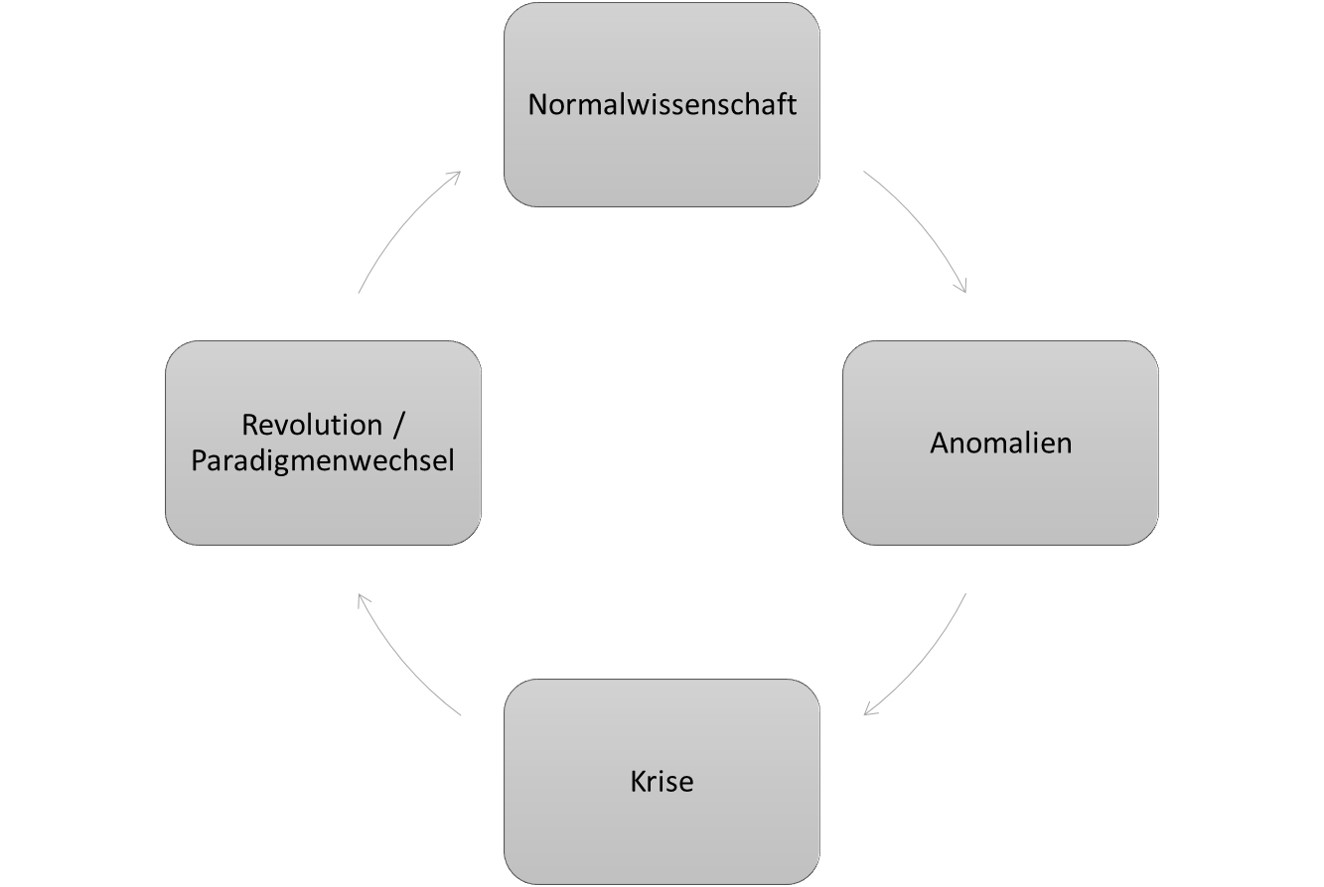
\includegraphics{images/paradigmenwechsel.jpg}

}

\caption{Wissenschaftliche Revolution nach (Kuhn 1970/1996), Darstellung
in Anlehnung an (Fiorentino and Montana Hoyos 2014)}

\end{figure}%

Ein Paradigmenwechsel ist vergleichbar mit einem Kippbild die dem
Hase-Ente-Bild (\textbf{Abbildung 1}) wie es zum Beispiel Wittgenstein
(1968) gezeichnet hat. Bis zu einem gewissen Punkt sind sich alle einig,
dass es ein Hase ist. Doch nach und nach kommen Erkenntnisse und
Perspektiven hinzu. Der Punkt wird überschritten, die Ente ist
anerkannt, und niemand würde es mehr für einen Hasen halten. Beim
Hase-Ente-Bild lässt sich natürlich beliebig hin und her springen. Beim
wissenschaftlichen \emph{Fortschritt} kommt neues Wissen hinzu und eine
Rückkehr ist nur noch schwer möglich.

\begin{figure}[H]

{\centering 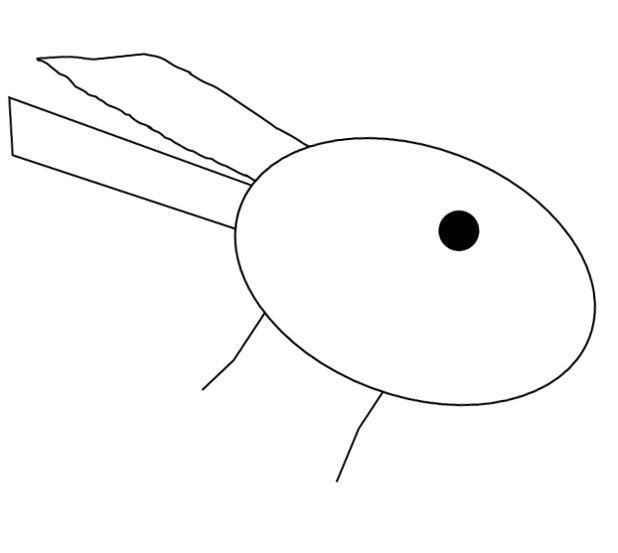
\includegraphics{images/entehase-01.jpg}

}

\caption{Hase-Ente-Kippbild frei nach Wittgenstein: Die Ausstülpungen
auf der linken Seite können entweder als Schnabel einer nach links
blickenden Ente oder als Ohren eines nach rechts blickenden Hasen
interpretiert werden.}

\end{figure}%

Forschende werden im Rahmen ihres Studiums oder einer Promotion von
Beginn an darin geschult, entsprechend des amtierenden Paradigmas mit
Befunden umzugehen.

\begin{tcolorbox}[enhanced jigsaw, title=\textcolor{quarto-callout-tip-color}{\faLightbulb}\hspace{0.5em}{Beim ersten Versuch klappt es nie: Paradigmenwechsel in der Psychologie}, colbacktitle=quarto-callout-tip-color!10!white, rightrule=.15mm, titlerule=0mm, left=2mm, bottomrule=.15mm, arc=.35mm, leftrule=.75mm, toprule=.15mm, opacityback=0, breakable, bottomtitle=1mm, colframe=quarto-callout-tip-color-frame, toptitle=1mm, opacitybacktitle=0.6, coltitle=black, colback=white]

Schon im Rahmen meines Studiums wurde ich geschult, mit dem amtierenden
Paradigma konform mit fehlgeschlagenen Replikationen umzugehen. Das fand
noch statt bevor sich die Replikationskrise herauskristallisierte. Bei
der ersten Studie, an der ich beteiligt war, replizierten wir
beispielsweise den Befund, dass bunte Mengen in ihrer Anzahl weniger
aussahen als einfarbige Mengen. Im Rahmen der Konsumentenpsychologie ist
das hinsichtlich Slogans wie ``viele viele bunte Smarties'' etwas
kontraintuitiv, es lässt sich aber gestaltpsychologisch plausibel
darlegen (Redden and Hoch 2009). Nachdem eine Gruppe von Kommilitoninnen
das Gegenteil herausfand, nämlich dass \emph{bunte Smarties tatsächlich
nach mehr aussahen als einfarbige Smarties}, konnten wir in zwei eigenen
Folgestudien nichts vom beiden nachweisen. Egal ob sich die Smarties in
Teller, Tassen, oder Schalen, befanden, egal ob es blaue, rote, gelbe,
oder bunte Schokolinsen waren, egal ob Mengen geschätzt oder Smarties
aus großen Flaschen in Gefäße geschüttet wurden: Unsere Versuchspersonen
ließen sich von der ``Buntheit'' nicht beeinflussen. In den folgenden
Jahren durfte ich als Tutor dann weitere Replikationsversuche
durchführen. Der betreuende Professor und mein Mentor erklärte: Ich habe
es eigentlich noch nie erlebt, dass die Hypothese gleich beim ersten
Versuch bestätigt wird. Nach jedem Experiment ist man schlauer und weiß,
was man nächstes Mal besser machen muss. Es ist ganz natürlich, dass es
ein paar Versuche dauert, bis man weiß, wie sich die Hypothese
bestätigen lässt. Nachdem wir sechs Studien mit insgesamt 1383
Versuchspersonen durchgeführt hatten, die Autoren der Originalstudie um
Rat gebeten hatten, haufenweise Schokolinsen verzehrt hatten, und die
Hypothese über alle Studien hinweg nicht bestätigt wurde, hatte ich das
Vertrauen in den Befund verloren.

Ungefähr sechs Jahre später dachte ich während meiner Promotionszeit an
die Studien zurück und diskutierte mit dem Professor. Im Rahmen der
Replikationskrise war klar: Wenn man mehrere Experimente durchführt und
die Hypothese eigentlich falsch ist, wird alleine durch den Zufall ab
und zu trotzdem die Hypothese bestätigt. Das ist vergleichbar damit,
dass selbst eine faire Münze sechs Mal hintereinander auf derselben
Seite landen kann. Wenn man jedoch 10 Münzen jeweils sechs Mal wirft,
ist es nicht selten, dass eine der 10 Münzen sechs Mal auf derselben
Seite landet. Aus dieser Perspektive hat das Zitat, dass die Ergebnisse
beim ersten Versuch eigentlich nie so rauskommen, wie man es sich
wünscht, einen bitteren Beigeschmack: Wenn die Hypothese falsch ist, ist
es tatsächlich unwahrscheinlich, dass sie dennoch bestätigt wird. Nicht
aber, wenn viele Studien durchführt. Dann ist es sogar zu erwarten, dass
irgendwann eine Studie die Hypothese - auch wenn sie eigentlich falsch
ist (!) - bestätigt. Die Studien haben wir gemeinsam mit einigen
Beteiligten schließlich veröffentlicht (Röseler, Felser, et al. 2020).

\end{tcolorbox}

\subsection{Literatur}\label{literatur-6}

\chapter{Struktur der
Vertrauenskrise}\label{struktur-der-vertrauenskrise}

Im Gespräch über Präregistrierungen -- eine Methode zur Erhöhung der
Replizierbarkeit eines Befundes -- entgegnete ein Kollege: ``Schön und
gut, aber solange sich das System nicht ändert, wird sich an
Replikationsraten nichts ändern.'' Wie lässt sich dieser Einwand
verstehen? Zäumen (bzw. trensen) wir dazu das Pferd von hinten auf:
Spätestens seit dem Reproducibility Project Psychology (Open Science
Collaboration, 2015) ist den meisten Psycholog*innen klar, dass es große
Probleme bei der Replizierbarkeit von Befunden gibt. Woher kommen diese
genau? Ein wichtiges Problem ist hierbei der \emph{Publikationsbias},
womit gemeint ist, dass bei der Veröffentlichung von wissenschaftlichen
Berichten eine Auswahl getroffen werden muss und dadurch nur bestimmte
Ergebnisse publiziert werden (z.B. Ergebnisse, die eine bestimmte
Theorie stützen). Dadurch steht ein verzerrtes Bild der Realität. Oft
schreiben Wissenschaftler*innen sogar nur bestimmte Befunde zu Berichten
zusammen. ``Fehlgeschlagene Experimente'', also solche, bei denen eine
Hypothese nicht bestätigt oder eine Theorie nicht gestützt werden
konnte, landen in der Schublade (engl. \emph{File-Drawer-Problem};
Rosenthal (1979); Theodore D. Sterling (1959)). In extremeren Fällen
bedienen sich Wissenschaftler*innen verschiedener größtenteils
anerkannter Methoden, die Daten so darzustellen, dass sie die Hypothese
stützen oder tun so, als ob das, was sich aus den Daten lesen lässt, von
Beginn an die Hypothese gewesen wäre (HARKing, Parsons et al. (2022)).
Aber was treibt Personen, die sich vor allem für den Beruf wegen ihres
Interesse an der Funktionsweise der Welt (oder im Falle der Psychologie
der Funktionsweise des Menschen) und wegen Ihrer Suche nach Wahrheit
entschieden haben dazu, die Wahrheit zu unbewusst zu schönen oder sogar
bewusst zu manipulieren? Am Anfang des komplexen Prozesses, welcher zur
Replikationskrise geführt hat, steht das aktuelle wissenschaftliche
System: Ein Großteil der in der Wissenschaft beschäftigten arbeitet
unter extremem Druck und prekären Arbeitsbedingungen. Um nach ein bis
zwei Jahren eine Vertragsverlängerung zu erhalten, müssen Publikationen
von Artikeln in möglichst angesehenen Fachzeitschriften nachgewiesen
werden. Diese kriegt man durch besonders aussagekräftige und spannende
Ergebnisse. Das Anreizsystem der Wissenschaft belohnt also nicht
Wahrheit, Genauigkeit, Bescheidenheit, oder Transparenz, sondern vor
allem diejenigen Dinge, die nicht in der Hand eine*r Wissenschaftler*in
liegen: Spannende und eindeutige Ergebnisse (Bakker, van Dijk, and
Wicherts 2012).

Der Prozess von prekären Arbeitsbedingungen bis zur niedrigen
Replikationsrate ist hier veranschaulicht. In den folgenden Kapiteln
werden die Probleme und Lösungsansätze im Detail diskutiert.

\textbf{Abbildung 2}

\begin{figure}[H]

{\centering 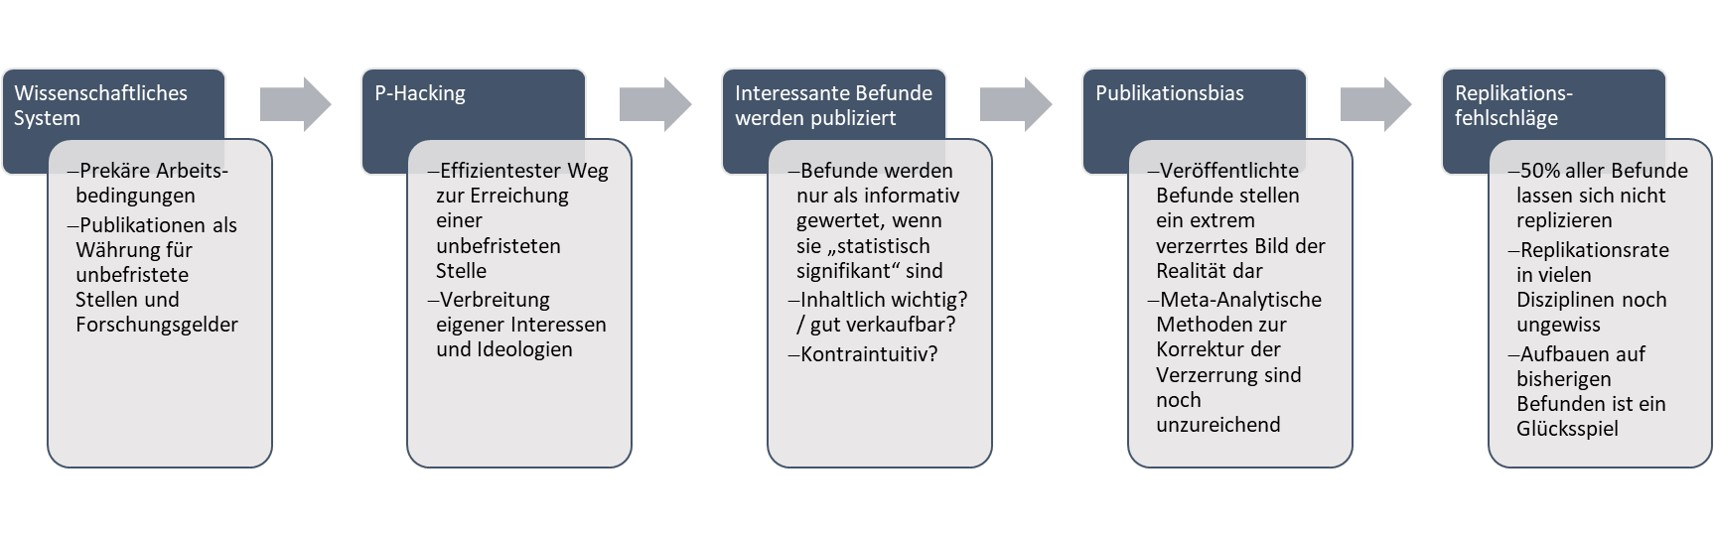
\includegraphics{images/struktur.jpg}

}

\caption{Das Anreizsystem der Wissenschaft als Ursache für
Replikationsfehlschläge}

\end{figure}%

\subsection{Literatur}\label{literatur-7}

\part{Probleme}

\part{Probleme, die im Rahmen der Revolution identifiziert wurden}

Im folgenden werden zahlreiche Probleme des Wissenschaftssystems erklärt
und aufgelistet. Manche der Probleme sind seit vielen Jahrzehnten
bekannt und andere erst seit wenigen Jahren. Es sei bei der Lektüre zu
beachten, dass es zu \emph{allen} diesen Problemen bereits
ausgearbeitete und teilweise auch ausgeführte Lösungsansätze gibt. Wie
die Lösungsansätze aussehen und welche Lösungen auf welche Probleme
zugeschnitten sind, wird ausführlich im Kapitel zu Lösungen erläutert.

\chapter{Das System}\label{das-system}

\section{Probleme des Wissenschaftlichen
Systems}\label{probleme-des-wissenschaftlichen-systems}

Neben dem Idealbild davon, was Wissenschaft sein sollte oder wie sie
funktionieren sollte, existiert die Wissenschaft, wie sie in unser
Gesellschaftssystem integriert ist. Besonderheiten sind dabei, dass
Wissenschaftler*innen ihre Tätigkeit als Beruf ausüben, also Geld dabei
verdienen. Wie das Geld, das größtenteils aus Steuergeldern stammt,
verteilt werden soll entscheiden Gremien, die wiederum selbst aus
Wissenschaftler*innen bestehen (\emph{akademische Selbstverwaltung}).
Durch die hohe Arbeitsbelastung, gleichzeitig Wissenschaft zu betreiben
und zu verwalten, vereinfachen sich die Entscheider*innen die Arbeit und
verwenden zur Auswahl hochqualifizierter Personen Abkürzungen. So konnte
es passieren, dass die Währung in der Wissenschaft zum Großteil die
Anzahl der in Fachzeitschriften veröffentlichten Forschungsartikel
(\emph{Paper}) ist. Ein weiterer verwendeter Indikator ist die Anzahl,
in wie vielen weiteren wissenschaftlichen Artikeln auf die Forschung
einer Person verwiesen wird, also die Zitationszahlen. Vorbilder wie
Charles Darwin oder William James und selbst aktuelle Nobelpreisträger
hätten nach dem heutigen Maßstab keine Chance auf eine unbefristete
Stelle in der Wissenschaft - sie haben einfach nicht genug Paper
geschrieben. Viele der hier diskutierten Problemen, sind beispielsweise
in der Psychologie seit mehreren Jahrzehnten bekannt, sodass eine
Replikationskrise unabwendbar erschienen haben muss (Cronbach, Snow, and
Wiley 1991; Greenwald 1976).

\subsection{Wissenschaft versus
Academia}\label{wissenschaft-versus-academia}

Während einige Natur- und Sozialwissenschaften in ihrer Anfangszeit oft
von Buchveröffentlichungen lebten und darin eine umfangreiche Basis von
meist einzelnen Personen erarbeitet wurde (z.B. Galileo Galilei für die
Physik oder William James für die Psychologie) stehen heutzutage
wissenschaftliche Fachzeitschriften im Fokus. Diese Zeitschriften sind
vergleichbar mit solchen, die es im Kiosk und im Supermarkt gibt, nur
bestehen sie halt aus (meist englischsprachigen) Artikeln, die
Wissenschaftler*innen verfasst haben und sind in vielen Fällen nur noch
online oder in Hochschulbibliotheken erhältlich. Forschende laden sich
dann einzelne Artikel aus den Zeitschriften aus dem Internet über das
Hochschulnetezwerk herunter und Bibliotheken haben Verträge mit Verlagen
und zahlen Geld, damit Universitätsangehörige Zugriff zu den Katalogen
haben. Jeder eingereichte Artikel befasst sich mit einer Fragestellung,
die von den Forschenden selbst festgelegt wurde (z.B. wie viele
psychologische Studien lassen sich im Mittel replizieren?). Darin werden
meistens Studien mit deren Ergebnissen berichtet. Vor der
Veröffentlichung werden die Artikel begutachtet (\emph{Review}) -- nicht
von Mitarbeitenden der Zeitschrift sondern von Kolleg*innen
(\emph{Peers}). Mit diesem \emph{Peer-Review} soll die Qualität von
Forschung sichergestellt werden. Üblicherweise wird dabei darauf
geachtet, dass die Schlussfolgerungen auf Basis der erhobenen Daten
gerechtfertigt sind, die Fragestellung klar beantwortet wird, der
Artikel verständlich ist, und die Befunde spannend oder überraschend
sind. Zeitschriften unterscheiden sich darin, welche Themen sie abdecken
(z.B. Sozialpsychologie, Konsumentenverhalten, Angewandte
Sportwissenschaft, usw.), wie streng das Peer-Review ist, und von wie
vielen Forschenden sie gelesen und zitiert werden. Wissenschaften sind
also stark integriert in ein System, das Forschenden und Verlagen
erlaubt, ein festes Gehalt zu verdienen.

\subsection{Prekäre Arbeitsbedingungen}\label{sec-arbeitsbedingungen}

Soweit der Rahmen: Wissenschaftler*innen forschen und teilen ihre
Ergebnisse meist in Form von \emph{Publikationen} wie
Zeitschriftenartikel- oder Buch-Veröffentlichungen. Was die Jobs in der
Wissenschaft (also vorwiegend an Hochschulen) angeht, so sind sie
hierarchisch strukturiert. Es gibt wenige unbefristete Stellen, meist
Professuren, und darunter befristete Stellen für Promovierende und
bereits promovierte \emph{Post Docs}. Wer in der Wissenschaft arbeitet,
befindet sich meistens in einem harten Konkurrenzkampf um eine der
wenigen unbefristeten Stellen (Rahal, Fiedler, Adetula, Berntsson,
Dirnagl, Feld, Fiebach, Himi, Horner, Lonsdorf, Schönbrodt, et al.
2023). Der Hintergedanke ist dabei, dass Konkurrenz zwischen Forschenden
die Produktivität steigern möge. Vom Start der Promotion\footnote{Prozess
  der Erlangung eines Doktorgrades/Doktortitles, je nach Disziplin und
  Hochschule durch das Verfassen eines Buches (Monografie) oder mehrerer
  Zeitschriftenartikel (kumulative Promotion)} bis zur Berufung auf eine
Professur, also eine der raren unbefristeten Stellen, dauern Verträge
meistens nur ein bis drei Jahre und haben oft einen Umfang von weniger
als 100\%. Gleichzeitig ist es unüblich ist, mit weniger als 40 Stunden
pro Woche innerhalb von den typischen drei Jahren die Promotion
erfolgreich abzuschließen. Während ein Großteil aller wissenschaftlichen
Veröffentlichungen auf Studien beruht, die im Rahmen von Doktorarbeiten
durchgeführt wurden, sind Doktorand*innen gleichzeitig diejenigen
Personen im System, die den geringsten Wert haben bzw. deren
Arbeitskraft am günstigsten ist. Forschende auf befristeten Stellen sind
also einem enormen Leistungsdruck ausgesetzt. Psychische Probleme wie
Burnout oder Depressionen sind unter Promovierenden weit verbreitet
(Jaremka et al. 2020; Liu et al. 2019). Den Weg zur Professur schaffen
vor allem die Personen erfolgreich, die viele Artikel in
prestigeträchtigen Zeitschriften veröffentlichen. Durch die immense
Arbeitsbelastung und große Zahl an Artikeln, die bei Fachzeitschriften
eingereicht werden, ist keine Zeit mehr, Ergebnisse genau zu prüfen und
nachzurechnen (Michele B. Nuijten et al. 2017), sondern es wird vor
allem darauf geachtet, wie eindeutig die Ergebnisse die Fragestellung
beantworten - oder genauer gesagt: bestätigen (Giner-Sorolla 2012;
Mynatt, Doherty, and Tweney 1977). Mit anderen Worten: Es wird
ausgerechnet der Teil der wissenschaftlichen Arbeit belohnt, der nicht
in der Hand der Forschenden liegt, nämlich die Ergebnisse von
Untersuchungen. Veröffentlichte Artikel und Prestige statt Qualität
(Brembs 2018) sind ab dort die Währung der Wissenschaft: Auf ihrer Basis
wird entschieden, wer Forschungsgelder erhält und auf Basis von
Forschungsgeldern und Publikationen werden Professuren vergeben. In den
darüber entscheidenden Berufungskommissionen lesen die Beteiligten
üblicherweise nicht die Artikel der Bewerbenden, sie zählen bloß, wie
viele in welchen Zeitschriften aufgelistet werden. Teilweise werden die
Bewerber*innen gebeten, Zitationszahlen anzugeben. Manche dieser Zahlen
(z.B. Impact Factor) gehören Unternehmen an und der Zugang muss über die
Institution erkauft werden.

Zu diesen verheerenden Problemen kommen außerdem systemische Probleme
der sexuellen Belästigung (Hoebel et al. 2022) und des
Machtmissbrauches, die in dem aktuell streng hierarchischen Aufbau des
Systems nur schwierig zu lösen sind (Forster and Lund (2018), siehe auch
\url{https://www.netzwerk-mawi.de/} und
\url{https://www.jmwiarda.de/2023/11/20/das-stille-leiden-der-betroffenen/}).
Berichten des Netzwerkes gegen Machtmissbrauch in der Wissenschaft
werden Fälle verschwiegen, und die schuldigen wechseln stillschweigend
die Universität, sodass das Problem nicht gelöst wird. Wer es dabei
besonders leicht hat, erklären M. M. Elsherif et al. (2022) anschaulich
an dem \emph{Academic Wheel of Privilege} (``Akademisches Rad der
Privilegierten''; S. 85; siehe auch
\url{https://www.psychologicalscience.org/observer/gs-navigating-academia-as-neurodivergent-researchers}).
Beispielsweise haben Doktorandinnen in den Niederlanden vor allem dann
schlechtere Noten als Doktoranden bekommen, wenn der
Promotionsausschuss, also die Gruppe an Professor*innen, die die
Promotion beurteilt, nur aus Männern bestand (Bol 2023).
Schwerbehindertenquoten weit unter den
\href{https://www.laborjournal.de/rubric/essays/essays2023/e23_09.php}{Quoten}
anderer Berufe kommen ebenfalls hinzu.

\subsection{\texorpdfstring{\textbf{Zu viel
Forschung}}{Zu viel Forschung}}\label{zu-viel-forschung}

Im Rahmen von Promotionen müssen Forschende in insgesamt 3-6 Jahren
zuzüglich Elternzeiten üblicherweise drei wissenschaftliche Artikel
veröffentlichen (bzw. in fairen Fällen drei
veröffentlichungs-\emph{würdige} Artikel vorweisen). Bei Post Docs
(siehe Section~\ref{sec-arbeitsbedingungen}) müssen es noch mehr sein.
Dass Personen vor und nach der Promotion jeweils maximal 6 Jahre an
Hochschulen angestellt sein dürfen ist gesetzlich festgelegt. Für die
weitere Qualifikation \emph{Habilitation}, für die eine ähnliche Zeit
angesetzt ist, sind zum Beispiel in der Psychologie circa 6 Artikel die
Daumenregel. Dabei spielt es eine nachrangige Rolle, wie umfangreich die
Artikel sind. Beispielsweise dauert die Durchführung einer Meta-Analyse,
in der bisherige Befunde zu einem bestimmten Thema systematisch
gesammelt und statistisch zusammengefasst bzw. verglichen werden, oft
mehrere Jahre. Eine Längsschnitterhebung kann je nach Forschungsfrage
sogar Jahrzehnte dauern. Im Kontrast dazu lässt sich eine
Querschnittserhebung über einen Online-Fragebogen in wenigen Wochen
durchführen. Eine Doktorandin, die eine einzige Meta-Analyse durchführt,
könnte damit nicht promovieren. Hätte sie stattdessen drei einfache
Online-Studien durchgeführt und einzeln veröffentlicht, wäre es
kein.\footnote{Hier ließe sich einwenden, dass einige Zeitschriften nur
  Artikel veröffentlichen, in denen mehrere Studien durchgeführt wurden.
  Das Ziel, nämlich die \emph{internale} Replikation der eigenen
  Befunde, verfehlen diese Zeitschriften damit deutlich. Stattdessen
  reizt es Forschende dazu an, mehrere Studien mit wenigen
  Versuchspersonen durchzuführen, statt eine Studie mit vielen
  Befragten.} Diese willkürlichen Vorgaben haben dazu geführt, dass sich
Wissenschaftler*innen alleine durch die Begutachtung der Artikel ihrer
Kolleg*innen einen enormen Arbeitsaufwand auferlegen, der den
wissenscchaftlichen Fortschritt behindert (Hanson et al. 2023).

Zur Veranschaulichung des Aufgabenpensums nun ein Gedankenspiel:
Angenommen es gäbe 10 Wissenschaftler*innen, die gemeinsam 10 Artikel im
Jahr veröffentlichen würden - manchmal alleine, manchmal in einer Gruppe
- und jeder der Artikel würde von zwei Personen begutachtet, so müsste
jede*r zwei Artikel begutachten. Damit das System funktioniert, müsste
jede Person die Anzahl der im Schnitt veröffentlichten Artikel mal die
Anzahl der benötigten Gutachtenden begutachten. Bei 10
Veröffentlichungen pro Person und drei Gutachtenden wären es 10x3=30
Gutachten. Nun werden aber nicht alle Artikel von der Zeitschrift, bei
der sie eingereicht werden, veröffentlicht, noch werden sie sofort
veröffentlicht. Wissenschaftler*innen reichen ihre Artikel oft bei den
``hochrangigsten'' Zeitschriften ein. Nachdem dort mehrere
Gutachter*innen den Artikel geprüft haben, wird er abgelehnt (Jaremka et
al. 2020). Im Mindestfall werden Revisionen angefordert, welche oft eine
weitere Runde Peer Review auslösen und nicht immer werden Artikel danach
veröffentlicht. Unsere Rechnung geht also nicht auf: Nehmen wir
\emph{vorsichtshalber} an, ein Artikel würde neun Mal begutachtet (z.B.
einmal drei Gutachtende, dann Ablehnung, dann erneut drei Gutachtende,
Revision, zweites Gutachten, Akzeptanz). Aus 10x3 wird 10x9, bei etwas
Urlaubszeit also etwas mehr als zwei Gutachten pro Woche, idealerweise
bis zu zwei Arbeitstage. Bei dieser Rechnung bleibt weniger Zeit für
Lehre, Wissenstransfer, Betreuung von Studierenden oder Promovierenden,
Einwerbung von Forschungsgeldern, universitäre Selbstverwaltung, usw.
Durch die vielen zu publizierenden Artikel und das strenge Review-System
bürgt sich die Wissenschaft einen großen Berg Arbeit auf -- einen der
realistisch nicht machbar ist und unter dem am Ende die Qualität der
Forschung leidet. Beispielsweise fiel es weder den Gutachtenden, noch
den Herausgebern von Zeitschriften auf, dass in über 30 Artikeln mitten
im Text „Regenerate response'' stand -- ein Satz, der in OpenAIs ChatGTP
Programm auf einem Knopf erlaubt, einen von einer künstlichen
Intelligenz erstellten Text umzuformulieren
(\url{https://retractionwatch.com/2023/10/06/signs-of-undeclared-chatgpt-use-in-papers-mounting/}).
In manchen Artikeln hieß es sogar „As an AI language model, I \ldots''
(\href{https://pubpeer.com/search?q=\%22As+an+AI+language+model\%2C+I}{https://pubpeer.com/search?q=``As+an+AI+language+model\%2C+I}``).
In einem Fall wurde der Artikel von dem Verlag Elsevier geändert, und
zwar nicht auf dem empfohlenen Weg\footnote{Ethische Richtlinien im
  Publikationsprozess sind zum Beispiel verfügbar über das Committee on
  Publication Ethics
  (\url{https://publicationethics.org/guidance/Guidelines}).} mittels
eines transparenten \emph{Errandum} oder \emph{Corrigendum}, also einer
öffentlichen Mitteilung über die Änderung und ihre Gründe, sondern ohne
Erklärung oder Zustimmung der Autor*innen
(\url{https://predatory-publishing.com/elsevier-changed-a-published-paper-without-any-explanation/}).

\subsection{Publish or Perish -- Veröffentlichen oder
Verenden}\label{publish-or-perish-veruxf6ffentlichen-oder-verenden}

Wer in der Wissenschaft arbeitet sollte die wichtigste Spielregel
kennen: Wer überleben will, muss Artikel veröffentlichen. Kurz:
Veröffentlichen oder Verenden (engl. \emph{publish or perish}). Zur
Promotion, Habilitation, Einwerbung von Forschungsgeldern, und zur
Berufung auf eine Professur sind Veröffentlichungen das oberste
Kriterium. Kennzeichen einer Währung ist, dass sich Dingen ein Wert
zuweisen lässt. Wie sieht der Wert in der Forschung aus?
Bibliometriker*innen entwarfen zur Beschreibung und zur Auswahl von
Zeitschriftenabonnements (also explizit \emph{nicht zur Bewertung})
verschiedener Forschungsgebiete verschiedene Kennzahlen, wie den Impact
Factor, oder Hirsch-Index. Beide Zahlen bestehen aus Verrechnungen
davon, wie oft Artikel je nach Zeitschrift oder je nach Person zitiert
wurden. Beispielsweise werden beim Journal Impact Factor die Gesamtzahl
der Zitationen in einem bestimmten Jahr durch die Anzahl der zitierbaren
Veröffentlichungen in Bezugsjahren (z.B. den 3 vorangegangenen Jahren)
geteilt. Zeitschriften werden mit hohen Impact Factors beworben und
erlauben teilweise nicht die Zitation von Kommentaren (bzw.
veröffentlichen Kommentare unter derselben Referenz wie
Originalstudien), um möglichst hohe Impact Factors zu erhalten. Sie
können natürlich auch entscheiden, ob sie den 3-Jahres- oder 2-Jahres
Impact Factor berichten. Berechnungsweisen unterscheiden sich außerdem
darin, auf Basis welcher Daten sie errechnet werden. Die Datenbank des
Journal Impact Factors gehört dem Unternehmen Clarivate Analytics und
ist nicht öffentlich zugängig. Das heißt, die genauen Zahlen lassen sich
nicht einfach nachrechnen und prüfen. Durch die wichtige und
intransparente Rolle von Zitationsmetriken ist wenig überraschend, dass
sie
\href{https://quantixed.org/2016/01/05/the-great-curve-ii-citation-distributions-and-reverse-engineering-the-jif}{manipuliert}
werden. Klar ist auch, dass Zitationsmetriken entweder gar nicht oder
negativ mit wissenschaftlicher Qualität zusammenhängen {[}Brembs (2018);
Etzel et al. (2024); Table 3{]}. Zum Beispiel gab es das Problem, dass
das Programm Microsoft Excel Genomnamen als Datumsangaben erkannt hat,
umformatiert hat, und die eigentlichen Namen nicht mehr erkennbar waren.
Somit waren Teile der jeweiligen Ergebnisse nutzlos (Ziemann, Eren, and
El-Osta 2016). Dieses Problem kam vor allem bei angesehenen
Zeitschriften vor. Sie haben nichts dagegen unternommen, stattdessen
wurde Excel nach ein paar Jahren angepasst.

Neben Zeitschriften können auch Ranglisten von Personen erstellt werden.
Forschende aus Stanford veröffentlichten eine solche Liste der \emph{20
meistzitierten Forschenden.} Abgesehen davon, dass sie zum Missbrauch
verführt, enthält zahlreiche Fehler (Abduh 2023) wie zum Beispiel
Forschende, die hunderte Jahre lang Artikel veröffentlicht haben -- vor
und nach ihrem Tod. Unternehmen, denen Verlage und andere Werkzeuge für
die Wissenschaft (z.B. Programme zur Verwaltung von Literatur) gehören,
sammeln darüber hinaus Daten über die Forschenden (z.B. welche Artikel
wie lange aufgerufen werden, welche Textpassagen markiert werden).
Teilweise werden Bibliotheken aufgefordert, Überwachungsprogramme von
Verlagen zu installieren. Die gesammelten Daten verkaufen die Verlage
dann zurück an die Forschenden. Diese Praxis gefährdet die
Wissenschaftsfreiheit, da Staaten Verlage auffordern können, die Namen
von Forschenden zu nennen, die zu politisch brisanten Themen forschen.
Die Initiative \href{https://stoptrackingscience.eu}{Stop Tracking
Science} setzt sich gegen das Verhalten ein.

Seit längerem wird für die verantwortungsvolle Verwendung dieser
Metriken plädiert (Hicks et al. 2015) und zahlreiche Universitäten und
Forschende tun sich zusammen um Bewertung von Forschung sinnvoll zu
gestalten (z.B. mittels der
\href{https://sfdora.org/read/read-the-declaration-deutsch/}{San
Francisco Erklärung zur Forschungsbewertung}). Wie sich Anreizstrukturen
und Karrierestatus auf wissenschaftliches Fehlverhalten auswirken, wird
mit gemischten Ergebnissen untersucht. Das Problem: Sobald es in einem
System ein klares Bewertungskriterium gibt, wird alles darauf
ausgerichtet (\emph{gaming the system}). Anreizstrukturen, die schlechte
Forschung zur Folge haben herrschen in Bezug auf Bildmanipulationen in
der Biologie laut Fanelli, Schleicher, et al. (2022) vor allem in China,
weniger jedoch in USA, Großbritannien, und Kanada.

Ein weiteres Produkt der \emph{Publish or Perish Struktur} ist, dass die
meisten in der Psychologie entwickelten Instrumente zur Messung von
Persönlichkeitseigenschaften nur wenige Male verwendet werden -- und das
auch hauptsächlich von ihren eigenen Entwickler*innen (Elson et al.
2023). Elson et al. (2023) plädieren: Psychologische Messinstrumente
sind keine Zahnbürsten! Ein noch extremeres Ausmaß ist bei sogenannten
\emph{Paper Mills} zu sehen (van Noorden 2023): Personen erstellen dabei
automatisiert große Mengen von wissenschaftlichen Artikeln, ohne die
darin beschriebenen Untersuchungen wirklich durchzuführen.
Wissenschaftler*innen können dann Ko-Autor*innenschaften kaufen, um ihre
Anzahl an veröffentlichten Artikeln zu erhöhen und mehr Zitationen zu
bekommen. Je nach Zeitschrift werden diese Artikel nicht im Peer-Review
entlarvt. Es wird befürchtet, dass Käufer*innen solcher Artikel selbst
sehr erfolgreich werden können, selbst Herausgeber von Zeitschriften
werden, und sich dadurch selbst schützen, ertappt zu werden. Der genaue
Ausmaß des Paper-Mill-Problems ist unklar und weitgehend unerforscht
(Byrne and Christopher 2020). Ein Indiz, mithilfe künstlicher
Intelligenz erstellte Artikel zu erkennen sind sogenannte \emph{tortured
phrases} (Cabanac, Labbé, and Magazinov 2021)\emph{,} welche grammatisch
korrekt sind, im üblichen Sprachgebrauch jedoch selten vorkommen oder
wenig Sinn machen.

\subsection{Flaschenhals-Hypothese und
Innovationsdrang}\label{flaschenhals-hypothese-und-innovationsdrang}

Namhafte wissenschaftliche Zeitschriften erhalten täglich unzählige
Einreichungen, veröffentlichen aber nur eine begrenzte Anzahl an
Artikeln. Sie müssen also streng selektieren, was begutachtet und
gegebenenfalls veröffentlicht wird. Weil das Ziel einer Zeitschrift ist,
viel gelesen zu werden, wählen Herausgeber*innen von Zeitschriften
diejenigen Artikel, welche möglichst großes Potenzial haben, bekannt und
viel zitiert zu werden (Giner-Sorolla 2012). Das betrifft zum Beispiel
Beiträge mit besonderen praktischen Implikationen, überraschenden
Befunden, oder besonders konsistenten Befunden. Studien, deren
Ergebnisse keine eindeutigen Schlüsse zulassen -- oder deren Autor*innen
mit zu großer Vorsicht Schlüsse ziehen -- kommen also nicht infrage. In
den Neurowissenschaften kommunizieren manche Zeitschriften
beispielsweise öffentlich, dass sie keine Replikationsstudien
veröffentlichen und nach Neuheit selektieren, während die meisten keine
Stellung dazu nehmen (Yeung 2017). In der Psychologie nahmen 2017 nur 33
von 1151 Zeitschriften Stellung dazu, dass sie Replikationen akzeptieren
(Martin and Clarke 2017). Zwar werden innovative Befunde dann häufiger
zitiert, die Zeitschrift erhält also mehr Leser*innen, mehr
Einreichungen, und damit mehr Geld über Abonnements und
Veröffentlichungskosten. Vielzitierte Artikel lassen sich jedoch
schlechter replizieren als weniger zitiert (Serra-Garcia and Gneezy
2021) und prestigereiche Zeitschriften sind Magneten für fragwürdige
Forschungspraktiken (Kepes et al. 2022) und nachweisbar gleichwertige
oder sogar qualitativ schlechtere Forschung (Brembs 2018).~

Wie kommt es dazu? Es ist die Rede von einem Flaschenhals
(\emph{Bottleneck}; viele Einreichungen aber wenige Veröffentlichungen).
Das führt gemeinsam mit dem Anreiz in eben solchen Zeitschriften zu
publizieren dazu, dass Forschende alle möglichen Mittel nutzen, um eine
Chance auf eine Publikation zu erhalten. In manchen Instituten gilt, wer
in einer bestimmten Zeitschrift veröffentlicht, erhält automatisch die
Bestnote auf die Promotion. Andere Institute erklären schon in der
Stellenausschreibung für eine Promotionsstelle, in welcher Zeitschrift
die Ergebnisse des Forschungsprojektes veröffentlicht werden müssen. Die
Tatsache, dass prestigereiche Zeitschriften \emph{Nature} oder
\emph{Science} vor allem Artikel mit klaren Botschaften veröffentlichen
- also Artikel, die auch häufiger gelesen werden (Stavrova et al. 2024)
- spornt also Forschende an, klare Ergebnisse zu erschaffen. Passt mal
ein Befund nicht zu der geprüften Hypothese, wird er entweder
manipuliert oder gar nicht veröffentlicht und landet in der Schublade.

\subsection{Schubladen-Problem}\label{schubladen-problem}

Seit mehreren Jahrzehnten ist bekannt, dass Wissenschaftler*innen vor
allem diejenigen Studien veröffentlichen, die ihre Theorien stützen
(Rosenthal 1979; T. D. Sterling 1959). Im Extremfall hat jemand zum
Prüfen einer Theorie fünf Studien durchgeführt, in nur einer davon die
Theorie bestätigt, und nur diese veröffentlicht. Andere Forschende, die
dann die (veröffentlichte) Literatur durchsuchen, sehen nur die
``erfolgreiche'' Studie. Es entsteht der Eindruck, dass die Theorie
stimmt, während die Mehrheit der Studien diesen Schluss eigentlich nicht
nahelegt. Dass Studienergebnisse natürlichen, statistischen Schwankungen
unterliegen führt dazu, dass bei vielen Studien auch eine dabei sein
kann, die das gewünschte Ergebnis zeit. Durch das Schubladen-Problem
konnten sich ganze Forschungsstränge entwickeln, die seit dem
Bewusstsein für Replikationsstudien komplett ausgestorben sind
(Brockman, 2022).

Für \emph{Meta-Analysen}, also Studien, die bisherige Befunde
zusammenfassen, wurden bereits verschiedene Methoden entwickelt, die
Stärke des Schubladen-Problems (engl. \emph{File-Drawer-Problem}) zu
prüfen. Auch Methoden, diese Verzerrung zu korrigieren, existieren
bereits vielzählige (Fisher, Tipton, and Zhipeng 2017; Hedges and Vevea
1996; Schimmack 2020; Simonsohn, Nelson, and Simmons 2014b; van Aert and
van Assen 2018). Allerdings funktioniert keine der Methoden in allen
möglichen Szenarien (Carter et al. 2019). Um eine Veröffentlichung der
fehlgeschlagenen Studien kommen Forschende also nicht herum.

In der Medizin gibt es den besonderen Fall, dass alle dort
durchgeführten Studien öffentlich registriert werden müssen. Bei einer
Veröffentlichung muss dann eine Registrierungsnummer angegeben werden.
Über öffentliche Angaben zu registrierten Studien lässt sich somit
nachverfolgen, welche Personen, Institutionen, oder Länder wie viele
ihrer tatsächlich durchgeführten Studien veröffentlichen. Forschende in
Berlin haben dazu eine Website mit einem sogenannten interaktiven
\emph{Dashboard} entwickelt, um die darüber gesammelten Daten
durchsuchen und abbilden zu können (Franzen et al. 2023; Riedel et al.
2022). Auf \url{https://quest-cttd.bihealth.org/} ist nach aktuellem
Stand (Juli 2024) sichtbar, dass von allen registrierten Studien nur
46\% innerhalb der folgenden zwei Jahre und 74\% innerhalb der folgenden
fünf Jahre veröffentlicht wurden. Personen, die sich für die Studien als
Versuchspersonen melden oder Drittmittelgeber erhalten somit Aufschluss
über die Größe der Schublade, in der die fehlgeschlagenen Studien und
die ``nicht so spannenden Ergebnisse landen''.

\subsection{Zugängigkeit von Wissen}\label{zuguxe4ngigkeit-von-wissen}

Durch die Einbindung von Forschung in das kommerzielle Verlagssystem
befindet sich ein Großteil der Wissenschaften in einem sozialen Dilemma,
das einen massiv eingeschränkten Zugang zum Wissen zur Folge hat. Das
vorherrschende Modell bei wissenschaftlichen Zeitschriften, die zum
Großteil Verlagen wie Springer, Elsevier, Sage, oder Taylor and Francis
angehören, ist ein Abonnement-Modell. Hochschul-Bibliotheken zahlen
Regelmäßig Geld an die Verlage, damit die Hochschul-Angehörigen (also
Studierende und Mitarbeitende) Zugriff auf die darin veröffentlichten
Arbeiten haben. Wer kein Abonnement hat, kann Artikel einzeln kaufen.
Versucht man, einen Artikel online herunterzuladen, ohne dass man sich
in einem Hochschulnetzwerk befindet, geht das nicht kostenlos: Der
Artikel befindet sich hinter einer Bezahlschranke (\emph{Paywall}). Soll
ein Artikel für alle frei zugänglich veröffentlicht werden (\emph{Open
Access},öffentlicher Zugang), kostet das extra, nämlich je Artikel
zwischen 2000€ und 9000€. Um Forschung also lesen zu können, müssen
Hochschulen Abonnements oder Artikel kaufen. Infolge dessen sind
finanziell schlechter ausgestattete Institutionen, Länder, oder sogar
gesamte Regionen wie der globale Süden in ihrer Teilnahme am
internationalen Wissenschaftsdiskurs systematisch benachteiligt.

Das soziale Dilemma besteht nun in der Schwierigkeit, dieses System zu
verändern. Brembs et al. (2023) beschreiben es wie folgt: Bibliotheken
schließen die Abos mit Verlagen ab, um Forschung an ihren Hochschulen zu
ermöglichen. Würden sie die Verträge kündigen, könnte das die Forschung
verlangsamen und die Stellung einer Hochschule verschlechtern.
Forschende können die namhaften Zeitschriften der kommerziellen Verlage
nicht boykottieren, da sie sonst ihre Karriere gefährden würden. Sie
sind darauf angewiesen, in prestigereichen Zeitschriften zu publizieren.
Zudem ist es extrem schwierig, das Verhalten von Millionen von
Forschenden, von denen die meisten viele Jahre lang mit dem aktuellen
System gelebt haben, schlagartig zu verändern. Die Zeitschriften, als
dritter Akteur in diesem Dilemma, profitieren von der Abhängigkeit und
können Preise beliebig steigen lassen. Abgesehen vom Markenwert der
Zeitschriften, also dem Ansehen und dem Vertrauen, das ihnen
fälschlicherweise (Brembs 2018) entgegengebracht wird, tragen sie zu
diesem System fast nichts bei. Universitäten und Länder haben bereits
jetzt die Möglichkeit, Forschungsartikel online zu verwalten; die
Begutachtung und Qualitätssicherung geschieht durch freiwillige
Forschende und nicht durch Angestellte der Zeitschrift; und die
Formatierung der Artikel können Forschende wie an bestehenden
\footnote{Damit sind Zeitschriften gemeint, die Artikel ohne
  Abonnement-Zugang und ohne Paywall veröffentlichen, und zwar ohne
  Kosten für die Autor*innen.} ersichtlich ist (Carlsson et al. 2017),
mit geringem Aufwand selbst übernehmen. Entsprechende Lösungen werden in
Section~\ref{sec-openaccess} erläutert.

\section{Vertiefende Informationen}\label{vertiefende-informationen-1}

Der kostenlose Film ``Paywall: The Business of Scholarship'' behandelt
das Thema Paywalls sowie den öffentlichem Zugang von wissenschaftlichem
Wissen: https://paywallthemovie.com/paywall

\section{Literatur}\label{literatur-8}

\chapter{Karriere in der
Wissenschaft}\label{karriere-in-der-wissenschaft}

Ein Beruf in der Wissenschaft setzt üblicherweise einen einschlägigen
Studienabschluss (Bachelor und Master) voraus und beginnt mit einer
Promotion. Im Rahmen der Promotion wird das wissenschaftliche Handwerk
erlernt und der Doktor*ingrad erlangt: Studien werden durchgeführt,
Daten analysiert, und Forschungsartikel veröffentlicht. In vielen Fällen
arbeiten Promovierende mit einer 50 -- 66\% Stelle als wissenschaftliche
Mitarbeiter*innen, begutachten für ihre Vorgesetzten Artikel und
Forschungsgelder-Anträge, schreiben eigene Anträge, verbringen mehrere
Monate im Ausland, erstellen, beaufsichtigen, und korrigieren Klausuren,
betreuen Abschlussarbeiten, und beteiligen sich an der universitären
Selbstverwaltung durch die Teilnahme an Sitzungen und Mitgliedschaften
bei Kommissionen. Zeitlich sind dabei bei Stellen oder Stipendien
üblicherweise drei Jahre angesetzt. Am Anfang meiner Promotion sagte man
mir, mit einer 40-Stunden-Woche schafft man es nicht, in der
vorgesehenen Zeit zu promovieren -- 50\% Gehalt für über 100\%
Arbeitszeit und einem befristeten Vertrag also. Verträge sind dabei
jedoch nicht immer auf die Zeit der Promotion befristet. Viele wissen
erst wenige Monate vor Vertragsende, wie viel Prozent Gehalt sie
erhalten, wie umfangreich die Lehrverpflichtung ist, und wie lange der
nächste Vertrag geht. Kurz: Die Arbeitsbedingungen sind nicht optimal
und man muss ein hohes Maß an Flexibilität mitbringen, wenn man sich für
den Weg in die Wissenschaft entscheidet.

\subsection{Doppelabhängigkeit}\label{doppelabhuxe4ngigkeit}

Für die Promotionsphase gibt es verschiedene Finanzierungsmöglichkeiten:
Über Unternehmen lässt sich berufsbegleitend promovieren oder Stipendien
zahlen über eine begrenzte Zeit Geld, das den Grunderhalt sichert (z.B.
1100€ über 36 Monate bei der Graduiertenförderung des Landes
Sachsen-Anhalt, dazu kommen noch zusätzliche Kosten für die
Sozialversicherung). Der häufigste Weg ist jedoch über eine Stelle als
wissenschaftliche*r Mitarbeiter*in. Dabei ist die vorgesetzte Person
diejenige Person, die auch die Promotionsarbeit bewertet. Die einem
auferlegte Korrektur der 120 Erstsemester-Klausuren steht dann im
Extremfall in Konflikt mit der Zeit, die für die Arbeit an der
wissenschaftlichen Studie benötigt wird. Promovierende hängen also
meistens von den betreuenden Professor*innen in Form der Beschäftigung
\emph{und} über die Bewertung ihrer Arbeit ab, was also als
\emph{Doppelabhängigkeit} bezeichnet wird.

\begin{tcolorbox}[enhanced jigsaw, title=\textcolor{quarto-callout-tip-color}{\faLightbulb}\hspace{0.5em}{Familienfeindliche Stipendien}, colbacktitle=quarto-callout-tip-color!10!white, rightrule=.15mm, titlerule=0mm, left=2mm, bottomrule=.15mm, arc=.35mm, leftrule=.75mm, toprule=.15mm, opacityback=0, breakable, bottomtitle=1mm, colframe=quarto-callout-tip-color-frame, toptitle=1mm, opacitybacktitle=0.6, coltitle=black, colback=white]

Unbefristete Stellen, Doppelabhängigkeit oder geringfügige Stipendien,
sowie Leistungsdruck haben klare negative Auswirkungen auf die
Gesundheit der Forschenden und damit auf die Qualität der Wissenschaft.
Wie sieht es mit Promotionsstipendien aus? Stipendien laufen oft 1 Jahr
mit Option auf Verlängerung oder bis zu 3 Jahre. Forschende, die direkt
nach der Schule und dem Studium promovieren, sind ca. 24 Jahre alt,
haben eventuell einen Partner, und wünschen sich eine Familie. Im Rahmen
ungewisser Vertragsverhältnisse ist das schwierig. Stipendien haben oft
keine Möglichkeit zur Elternzeit und müssen dann pausiert werden -- oder
sie laufen weiter und es wird keine zusätzliche Zeit angehängt. Sie
verbieten zusätzliches Einkommen, weshalb das Elterngeld dann auf den
dafür angesetzten Mindestbetrag fällt. Zusätzlich schreiben Sie vor,
dass die geförderte Person \emph{inklusive Ehepartner} ein bestimmtes
Maximalvermögen nicht überschreiten darf, sodass auch keine Finanzierung
durch mögliche Rücklagen klappt.

\end{tcolorbox}

\subsection{Depressionen, Burnout, und
\#IchbinHanna}\label{depressionen-burnout-und-ichbinhanna}

Fächerübergreifend hat sich als Antwort auf ein inzwischen gelöschtes
Erklärvideo vom Bundesministerium für Bildung und Forschung zum
Wissenschaftszeitvertragsgesetz (WissZeitVG) eine Bewegung unter dem
Hashtag \#IchbinHanna entwickelt, die die dortige sachliche Erklärung
(\url{https://www.youtube.com/watch?v=PIq5GlY4h4E}) und die
Arbeitsbedingungen in der Wissenschaft stark kritisiert. Es heißt „damit
auch nachrückende Wissenschaftlerinnen und Wissenschaftler die Chance
auf den Erwerb dieser Qualifizierung haben und nicht eine Generation
alle Stellen verstopft, dürfen Hochschulen und Forschungseinrichtungen
befristete Verträge nach den besonderen Regeln des WissZeitVG
abschließen. So kommt es zur Fluktuation und die fördert die
Innovationskraft''. 90\% aller Wissenschaftler*innen sind unbefristet
angestellt (\url{https://www.youtube.com/watch?v=H1wJmqpGhJc}).

Planungsunsicherheit und massiver Konkurrenzdruck fördern die
Innovationskraft? Das scheint unwahrscheinlich: Unter Forschenden
mentale Erkrankungen wie Burnout (Jaremka et al. 2020) und Anzeichen für
Angststörungen und Depression stark verbreitet. Einer Überblicksstudie
von Satinsky et al. (2021) zufolge, leiden zwischen 18 und 31\% der
Promovierenden unter Depressionen.

\begin{tcolorbox}[enhanced jigsaw, title=\textcolor{quarto-callout-caution-color}{\faFire}\hspace{0.5em}{Wer hilft?}, colbacktitle=quarto-callout-caution-color!10!white, rightrule=.15mm, titlerule=0mm, left=2mm, bottomrule=.15mm, arc=.35mm, leftrule=.75mm, toprule=.15mm, opacityback=0, breakable, bottomtitle=1mm, colframe=quarto-callout-caution-color-frame, toptitle=1mm, opacitybacktitle=0.6, coltitle=black, colback=white]

Schnelle Hilfe bei psychischen Problemen leistet beispielsweise das
Krisentelefon der
\href{https://www.telefonseelsorge.de}{TelefonSeelsorge}. Manche
Universitäten haben spezifische Anlaufstellen, Städte haben häufig
örtliche Psychotherapie-Ambulanzen und Beratungsstellen.

\end{tcolorbox}

\subsection{Top-Down-Wandel}\label{top-down-wandel}

Diejenigen, die das System ändern können, also alle mit unbefristeten
Verträgen, leiden nicht mehr unter ihm. Für diejenigen, die unter dem
System leiden, ist es unklug, das System ändern zu wollen und sich an
die Professor*innen zu wenden, denn das sind die Leute, die über ihren
späteren Verbleib in der Wissenschaft im Rahmen von
Berufungskommissionen bei der Entscheidung der Vergabe von Professuren
entscheiden. Im Extremfall kann das dazu führen, dass jemand Kritik an
Arbeiten von Wissenschaftler*innen in höheren Positionen aus Angst, die
eigenen Chancen auf eine Professur zu schmälern, zurückfährt. Auf der
anderen Seite haben Professor*innen bewiesen, dass sie sehr gut nach den
Spielregeln spielen können. Zuzugeben, dass sie eine der seltenen und
heiß begehrten Stellen nicht über Qualität sondern Quantität ihrer
Forschung erhalten haben, hieße, sich selbst abzuwerten.

\subsection{Literatur}\label{literatur-9}

\chapter{Methoden}\label{methoden}

Im Alltagsdenken herrscht noch oft der Mythos, dass Wissenschaft sich
von Nicht-Wissenschaft durch \emph{die wissenschaftliche Methode}
unterscheide. Das ist falsch (Feyerabend 1975/2002). Zwar unterscheidet
sich wissenschaftliches Wissen von alltäglichem Wissen (und auch
Religion) durch einen höheren Grad an Systematizität (Hoyningen-Huene
2013), allerdings gibt es weder eine einzige noch eine konstante
wissenschaftliche Methode. Methoden haben sich stattdessen über die Zeit
gewandelt, und das ist auch gut so. Neue Technologien ermöglichen
beispielsweise in der Physik hochpräzise Messungen mittels
Elektronenlaser, in den Geschichtswissenschaften 3D-Scans von
Artefakten, die sonst nur wenige sehen würden, oder in den
Sozialwissenschaften Datenbanken mit freiwillig bereitgestellten und
anonymisierten Chatverläufen (\url{https://db.mocoda2.de/c/home}).

So wie ein Hammer und andere Werkzeuge nicht gut oder schlecht sind, so
sind auch Methoden nicht gut oder schlecht, nicht richtig oder falsch,
sondern sie werden \emph{angemessen und korrekt} verwendet oder
missbraucht. Statt Missbrauch ist in den Sozialwissenschaften von
fragwürdigen Forschungspraktiken (\emph{Questionable Research
Practices}), kurz QRP, die Rede. Sie erlauben Wissenschaftler*innen
Befunde zu generieren, die sie wollen. Im Folgenden werden verbreitete
und oft angewandte (John, Loewenstein, and Prelec 2012) Techniken
vorgestellt (für einen Überblick über die Forschung dazu in den letzten
50 Jahren, siehe auch Neoh et al. (2023)).

\subsection{Exploratorische versus konfirmatorische
Forschung}\label{exploratorische-versus-konfirmatorische-forschung}

Zum Verständnis der fragwürdigen Forschungspraktiken (QRP) ist eine
wichtige forschungstechnische Unterscheidung unabdingbar: Wie bei einem
Spaziergang kann eine wissenschaftliche Untersuchung erkundend oder
zielgerichtet sein. Mal wird frei durch die Gegend spaziert und dabei
neue Entdeckungen gemacht, mal ist das Ziel und die Route klar und im
Vorhinein bestimmt. Im wissenschaftlichen Kontext ist die Rede von
exploratorischer und konfirmatorischer Forschung. Bei der Exploration
stehen höchstens die Forschungsfrage und grobe Züge der Methode fest,
bei einem konfirmatorischen Test ist alles durchdacht: Vorgehen,
mögliche Ergebnisse, sowie Erklärungsansätze für jedes mögliche
Resultat. Es wird dann eine spezifizierte Hypothese mit der
dazugehörigen Theorie bestätigt oder eben nicht. Kein Vorgehen ist dem
anderen überlegen. Üblicherweise beginnen Untersuchungen in einem bisher
wenig erschlossenen Gebiet mit Exploration, während mehr vorhergehende
Forschung mit klareren Erwartungen einhergeht. Es sei dazu gesagt, dass
es sich hier um Extremtypen von Forschung handelt, die ein Spektrum
bilden. Es erlauben außerdem erst beide Ansätze zusammen
Erkenntnisgewinn. Im Rahmen des hermeneutischen Zirkel, (einfach gesagt
``dem Kreis des Verstehens'') wird aus einzelnen Beobachtungen eine
allgemeine Gesetzmäßigkeit formuliert (\emph{Induktion}) und diese
Gesetzmäßigkeit wird im Anschluss bei weiteren Einzelbeobachtungen
geprüft (\emph{Deduktion}). Die Deduktion kann je nach Gesetzmäßigkeit
logisch notwendig sein, denn es wird von Prämissen auf eine Konklusion
geschlossen. Wenn beide Prämissen korrekt sind, muss also auch die
Schlussfolgerung korrekt sein. Die Induktion ist keine Notwendigkeit
(siehe \emph{Induktionsproblem}, Hume (1748/2011)).

\begin{figure}[H]

{\centering 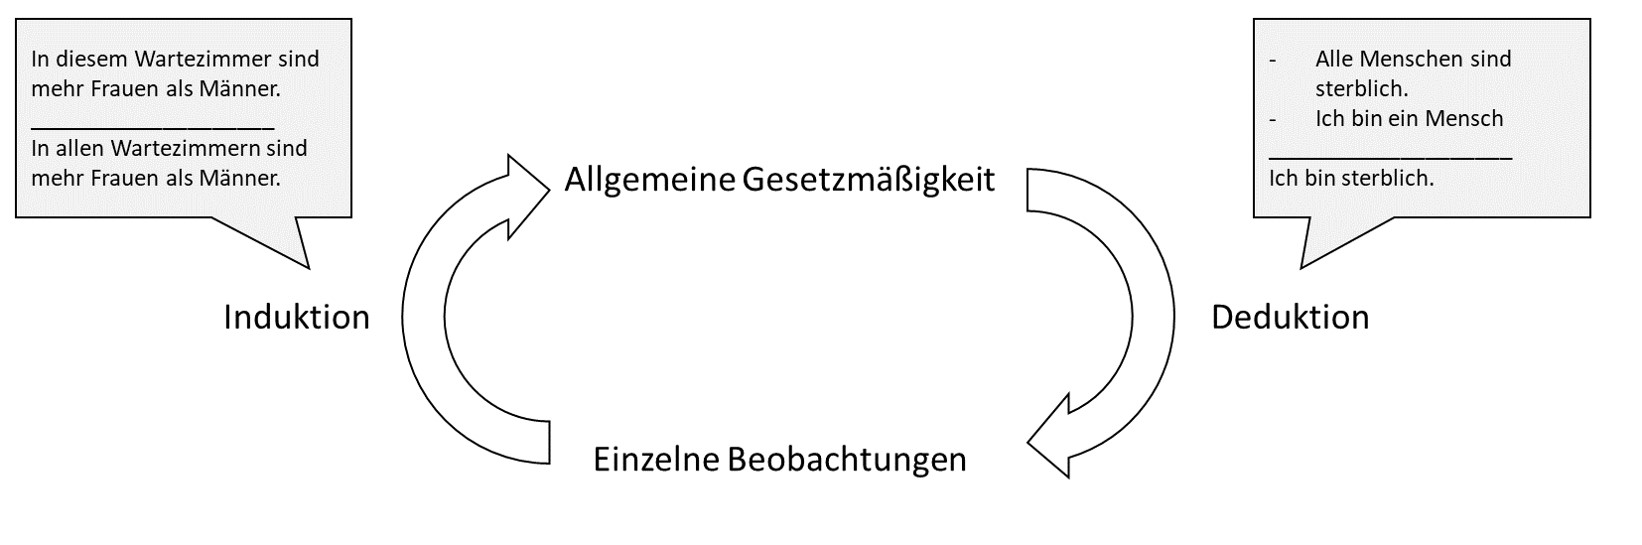
\includegraphics{images/hermeneutischerzirkel.jpg}

}

\caption{Hermeneutischer Zirkel}

\end{figure}%

Problematisch wird es, wenn exploratorische Forschung als
konfirmatorische kommuniziert wird, also so getan wird, als hätte eine
Einzelbeobachtung eine bereits formulierte Gesetzmäßigkeit bestätigt,
statt sie bloß inspiriert. Diese Art Unlogik heißt Zirkelschluss: Die
Gesetzmäßigkeit gilt wegen der Beobachtung. Und die Beobachtung
entspricht der Gesetzmäßigkeit.

\textbf{Abbildung Z}

\emph{Skizziertes Vorgehen bei explorativer (a) versus konfirmatorischer
(b) Forschung. Exploratives Vorgehen ist nicht zielgerichtet, die
Richtung kann sich ändern, und ist manchmal mit unvorhergesehenen
Ergebnissen verbunden. Konfirmatorisches Vorgehen bildet oft einen engen
und kontrollierten Ausschnitt eines Sachverhaltes ab.}

\subsubsection{Methoden der
Datengenerierung}\label{methoden-der-datengenerierung}

Wissenschaftliche Disziplinen bedienen sich für gewöhnlich vieler
verschiedener Methoden. Idealerweise sind Erkenntnisse unabhängig von
der Methode, die zu ihrer Entdeckung geführt hat und verschiedene
Methoden führen zur selben Erkenntnis. Typische sozialwissenschaftliche
Methoden sind die Befragung mittels standardisiertem Fragebogen,
Verhaltensbeobachtung mittels Kameraaufzeichnungen und anschließender
Kodierung von Verhaltensweisen durch mehrere Personen, die den
Untersuchungszweck nicht kennen, indirekte Methoden (Schimmack 2019),
bei welchen etwas anderes gefragt wird, als was gemessen werden soll,
Verhaltensmessungen wie Blickrichtungsmessung (\emph{eye tracking}),
oder Simulationsstudien, mittels derer zum Beispiel Verkehrsflüsse auf
Basis vorher festgelegter Prinzipien per Computer berechnet werden oder
Panikattacken vorhergesagt werden (Robinaugh et al. 2021). Diese
Methoden generieren fast immer Daten, also beispielsweise eine Tabelle,
in der je Beobachtungseinheit (z.B. je Versuchsperson) in mehreren
Spalten Daten festgehalten werden und diese Daten werden fast immer
statistisch ausgewertet. Die Notwendigkeit einer solchen Auswertung
ergibt sich daraus, dass die Beobachteten Gesetzmäßigkeiten keine
absoluten Gesetze im Sinne von „alle männlichen Babys wiegen mehr als
alle weiblichen Babys'' sind, sondern statistische Regelmäßigkeiten im
Sinne von „im Mittel wiegen kurz nach der Geburt männliche Babys ein
paar hundert Gramm mehr als weibliche Babys, aber nicht jedes männliche
Baby wiegt mehr als jedes weibliche Baby'' sind. Ein Vergleich von
Körpergrößen nach Geschlecht ist über
\href{https://de.statista.com/statistik/daten/studie/1825/umfrage/koerpergroesse-nach-geschlecht/}{Statista}
zu sehen.

In der folgenden Abbildung sind die Häufigkeiten verschiedener Werte zu
sehen (\emph{Histogramm}). Je weiter rechts ein Wert ist, desto höher
ist der Wert (z.B. Geburtsgewicht) und je höher der Balken ist, desto
häufiger kommt der Wert vor. Die gelbe und die lilane Verteilung
überlappen einander, das heißt, dass nicht alle gelben Werte niedriger
als alle lilanen sind. Im Mittel, sind die gelben Werte jedoch geringer.

\begin{Shaded}
\begin{Highlighting}[]
\FunctionTok{set.seed}\NormalTok{(}\DecValTok{1}\NormalTok{)}
\NormalTok{x }\OtherTok{\textless{}{-}} \FunctionTok{rnorm}\NormalTok{(}\DecValTok{1000}\NormalTok{, }\AttributeTok{mean =} \DecValTok{0}\NormalTok{)}
\NormalTok{y }\OtherTok{\textless{}{-}} \FunctionTok{rnorm}\NormalTok{(}\DecValTok{1000}\NormalTok{, }\AttributeTok{mean =} \DecValTok{1}\NormalTok{)}
\FunctionTok{hist}\NormalTok{(x, }\AttributeTok{xlim =} \FunctionTok{c}\NormalTok{(}\SpecialCharTok{{-}}\DecValTok{3}\NormalTok{, }\DecValTok{5}\NormalTok{), }\AttributeTok{col =} \FunctionTok{rgb}\NormalTok{(}\DecValTok{1}\NormalTok{,}\DecValTok{1}\NormalTok{,}\DecValTok{0}\NormalTok{,.}\DecValTok{2}\NormalTok{), }\AttributeTok{ylim =} \FunctionTok{c}\NormalTok{(}\DecValTok{0}\NormalTok{, }\DecValTok{40}\NormalTok{), }\AttributeTok{breaks =} \DecValTok{100}\NormalTok{, }\AttributeTok{xaxt =} \StringTok{"n"}\NormalTok{, }\AttributeTok{yaxt =} \StringTok{"n"}
\NormalTok{     , }\AttributeTok{xlab =} \StringTok{"Wert"}\NormalTok{, }\AttributeTok{ylab =} \StringTok{"Häufigkeit"}\NormalTok{, }\AttributeTok{main =} \StringTok{""}\NormalTok{)}
\FunctionTok{hist}\NormalTok{(y, }\AttributeTok{add =}\NormalTok{ T, }\AttributeTok{col =} \FunctionTok{rgb}\NormalTok{(}\DecValTok{1}\NormalTok{,}\DecValTok{0}\NormalTok{,}\DecValTok{1}\NormalTok{,.}\DecValTok{2}\NormalTok{), }\AttributeTok{breaks =} \DecValTok{100}\NormalTok{)}
\end{Highlighting}
\end{Shaded}

\includegraphics{probleme_methoden_files/figure-pdf/unnamed-chunk-1-1.pdf}

\begin{tcolorbox}[enhanced jigsaw, title=\textcolor{quarto-callout-note-color}{\faInfo}\hspace{0.5em}{Statistische Signifikanz}, colbacktitle=quarto-callout-note-color!10!white, rightrule=.15mm, titlerule=0mm, left=2mm, bottomrule=.15mm, arc=.35mm, leftrule=.75mm, toprule=.15mm, opacityback=0, breakable, bottomtitle=1mm, colframe=quarto-callout-note-color-frame, toptitle=1mm, opacitybacktitle=0.6, coltitle=black, colback=white]

Eine der am weitesten verbreiteten Methoden in den Sozialwissenschaften
(und auch darüber hinaus) ist Statistik, genauer
\emph{Inferenzstatistik}. Dabei wird von einer begrenzten Menge von
Beobachtungen (z.B. ausgefüllte Fragebogen von 100 Personen) auf alle
möglichen Beobachtungen (z.B. alle Menschen) verallgemeinert.
Untersuchte Zusammenhänge sind selten eindeutig, es gibt aber häufig
statistische Regelmäßigkeiten. Charakteristisch ist dabei ein gewisses
\emph{Zufallselement}. Wiegt man ein kürzlich geborenes männliches und
weibliches Baby, dann ist die Wahrscheinlichkeit sehr hoch, dass das
männliche Baby mehr wiegt. Es kommt aber auch häufig vor, dass das nicht
der Fall ist. Ähnlich verhält es sich bei einer fairen Münze, also einer
die im Mittel gleich häufig auf Kopf und auf Zahl landet: Dass sie bei
insgesamt vier Würfen immer auf Kopf landet ist unwahrscheinlich, dass
sie 1 oder 2 Mal auf Kopf landet, es kommt aber durch aus vor (nämlich
in 12,5\% aller Fälle, in denen eine faire Münze vier Mal hintereinander
geworfen wird).

Inferenzstatistische Tests gehen nun davon aus, dass bei der Betrachtung
eines statistischen Zusammenhanges (z.B. Geschlecht und Geburtsgewicht,
Körpergewicht und Größe, Bildungsniveau der Eltern und Bildungsniveau
der Kinder) „nur der Zufall am Werk ist'' (Röseler and Schütz 2022).
Unter der Annahme wird berechnet, wie häufig ein beobachteter
Zusammenhang mit der beobachteten Stärke vorkommen würde, wenn
\emph{eigentlich} kein Zusammenhang vorliegen würde. Also zum Beispiel
„dass eine faire Münze vier Mal auf Kopf landet, passiert in 12,5\%
aller Fälle''. Bei sechs Würfen wären es 1,5625\%. Die Kunst des
statistischen Schließens besteht nun darin, den Punkt zu finden, ab dem
Forschende davon ausgehen, dass der Zufall nicht am Werk war, weil die
berechnete Wahrscheinlichkeit so gering ist. Konventionell liegt dieser
bei 5\%, für neue Befunde manchmal bei 0,5\% (Benjamin et al., 2018),
und in besonders prekären Fällen noch niedriger. Fachtechnisch wird von
einem \emph{Alpha-Niveau} oder einem \emph{Signifikanzniveau} gesprochen
und die berechnete Wahrscheinlichkeit heißt \emph{p}-Wert. P-Werte unter
5\% werden \emph{statistisch signifikant} oder \emph{auf dem 5\%-Niveau
signifikant} bezeichnet. Forschende würden also sagen, dass eine Münze
\emph{nicht} fair ist, wenn sie sechs Mal hintereinander auf Kopf landet
(sogar schon bei fünf Mal, was in 3,125\% der Fälle vorkommt). Dabei
nehmen sie in Kauf, dass sie, wenn die Münze eigentlich doch fair ist,
in 5\% aller Fälle falsche Schlüsse ziehen.

Auf der anderen Seite ist es durchaus möglich, dass eine Münze nicht
fair ist, zum Beispiel in 60\% der Fälle auf Kopf landet und in 40\% auf
Zahl.~

\begin{figure}[H]

{\centering 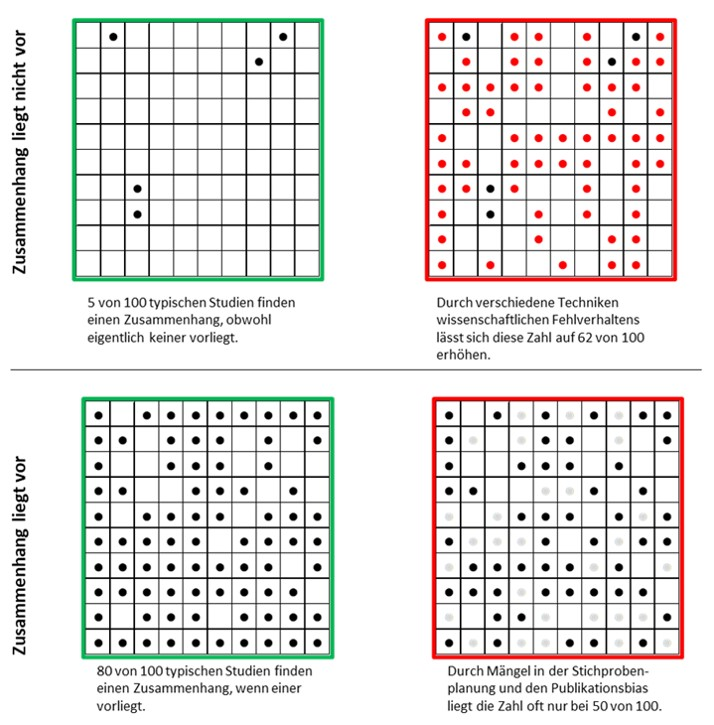
\includegraphics{images/freiheitsgrade.jpg}

}

\caption{Eine einzelne Studie führt noch nicht zu sicherer Erkenntnis.
Auch, wenn ein untersuchter Zusammenhang nicht vorliegt, kann er in
Daten zufällig aufscheinen. Und auch, wenn eigentlich ein Zusammenhang
vorliegt, kann dieser in den Daten durch Zufallsschwankungen nicht zu
erkennen sein. Mithilfe von Open Science Praktiken soll der Zustand in
den linken Kästen wiederhergestellt werden. Aus Röseler,~L. (2021).
Wissenschaftliches Fehlverhalten {[}Abbildung{]}. https://osf.io/uf7gz/.
Lizenziert unter CC BY-Attribution International 4.0.}

\end{figure}%

\end{tcolorbox}

\subsection{\texorpdfstring{Freiheitsgrade von Forschenden
(\emph{Researchers' Degrees of
Freedom})}{Freiheitsgrade von Forschenden (Researchers' Degrees of Freedom)}}\label{freiheitsgrade-von-forschenden-researchers-degrees-of-freedom}

Vollständige Studien mehrfach durchzuführen ist sehr aufwändig. Obwohl
es ein relativ sicherer Weg zu signifikanten P-Werten ist, gibt es
weitaus sparsamere Lösungen. Die meisten Analysen sind um ein vielfaches
komplexer als die oben beschriebene Münzwurfstudie. Betrachten wir den
immer noch sehr einfachen Signifikanztest für einen
Korrelationskoeffizienten. Der Koeffizient ist eine Zahl zwischen -1 und
1 und beschreibt die Art des Zusammenhanges zwischen zwei Variablen
(z.B. Einkommen und Lebenszufriedenheit). 0 bedeutet, dass kein
Zusammenhang vorliegt, positive Werte bedeuten, dass wenn die eine
Variable hohe Werte hat, dann hat auch die andere hohe Werte, und
negative Korrelationen bedeuten, dass wenn eine Variable hohe Werte hat,
dann hat die andere Variable eher niedrige Werte. In Abbildung X sind
verschiedene Korrelationen dargestellt.

\textbf{Verschiedene Zusammenhänge zwischen zwei Variablen und deren
Korrelationskoeffizienten (simulierte Daten).}

\begin{Shaded}
\begin{Highlighting}[]
\FunctionTok{layout}\NormalTok{(}\FunctionTok{matrix}\NormalTok{(}\FunctionTok{c}\NormalTok{(}\DecValTok{1}\NormalTok{, }\DecValTok{1}\NormalTok{, }\DecValTok{2}\NormalTok{, }\DecValTok{2}\NormalTok{, }\DecValTok{3}\NormalTok{, }\DecValTok{3}\NormalTok{, }\DecValTok{4}\NormalTok{, }\DecValTok{4}\NormalTok{), }\AttributeTok{nrow =} \DecValTok{2}\NormalTok{, }\AttributeTok{byrow =} \ConstantTok{TRUE}\NormalTok{)) }
\FunctionTok{set.seed}\NormalTok{(}\DecValTok{42}\NormalTok{)}
\NormalTok{n }\OtherTok{\textless{}{-}} \DecValTok{100}

\NormalTok{x1 }\OtherTok{\textless{}{-}} \FunctionTok{rnorm}\NormalTok{(n)}
\NormalTok{y1 }\OtherTok{\textless{}{-}} \FunctionTok{rnorm}\NormalTok{(n)}
\NormalTok{y2 }\OtherTok{\textless{}{-}}\NormalTok{ x1}\SpecialCharTok{+}\FunctionTok{rnorm}\NormalTok{(n)}
\NormalTok{y3 }\OtherTok{\textless{}{-}} \SpecialCharTok{{-}}\NormalTok{x1}\SpecialCharTok{+}\FunctionTok{rnorm}\NormalTok{(n)}
\NormalTok{y4 }\OtherTok{\textless{}{-}} \FunctionTok{abs}\NormalTok{(x1}\SpecialCharTok{+}\FunctionTok{rnorm}\NormalTok{(n))}\SpecialCharTok{\^{}}\DecValTok{2}

\FunctionTok{plot}\NormalTok{(x1, y1, }\AttributeTok{main =} \FunctionTok{paste}\NormalTok{(}\StringTok{"r = "}\NormalTok{, }\FunctionTok{round}\NormalTok{(}\FunctionTok{cor}\NormalTok{(x1, y1), }\DecValTok{2}\NormalTok{), }\AttributeTok{sep =} \StringTok{""}\NormalTok{)}
\NormalTok{     , }\AttributeTok{xaxt =} \StringTok{\textquotesingle{}n\textquotesingle{}}\NormalTok{, }\AttributeTok{yaxt =} \StringTok{\textquotesingle{}n\textquotesingle{}}\NormalTok{, }\AttributeTok{xlab =} \StringTok{""}\NormalTok{, }\AttributeTok{ylab =} \StringTok{""}\NormalTok{, }\AttributeTok{pch =} \DecValTok{20}\NormalTok{)}
\FunctionTok{plot}\NormalTok{(x1, y2, }\AttributeTok{main =} \FunctionTok{paste}\NormalTok{(}\StringTok{"r = "}\NormalTok{, }\FunctionTok{round}\NormalTok{(}\FunctionTok{cor}\NormalTok{(x1, y2), }\DecValTok{2}\NormalTok{), }\AttributeTok{sep =} \StringTok{""}\NormalTok{)}
\NormalTok{     , }\AttributeTok{xaxt =} \StringTok{\textquotesingle{}n\textquotesingle{}}\NormalTok{, }\AttributeTok{yaxt =} \StringTok{\textquotesingle{}n\textquotesingle{}}\NormalTok{, }\AttributeTok{xlab =} \StringTok{""}\NormalTok{, }\AttributeTok{ylab =} \StringTok{""}\NormalTok{, }\AttributeTok{pch =} \DecValTok{20}\NormalTok{)}
\FunctionTok{plot}\NormalTok{(x1, y3, }\AttributeTok{main =} \FunctionTok{paste}\NormalTok{(}\StringTok{"r = "}\NormalTok{, }\FunctionTok{round}\NormalTok{(}\FunctionTok{cor}\NormalTok{(x1, y3), }\DecValTok{2}\NormalTok{), }\AttributeTok{sep =} \StringTok{""}\NormalTok{)}
\NormalTok{     , }\AttributeTok{xaxt =} \StringTok{\textquotesingle{}n\textquotesingle{}}\NormalTok{, }\AttributeTok{yaxt =} \StringTok{\textquotesingle{}n\textquotesingle{}}\NormalTok{, }\AttributeTok{xlab =} \StringTok{""}\NormalTok{, }\AttributeTok{ylab =} \StringTok{""}\NormalTok{, }\AttributeTok{pch =} \DecValTok{20}\NormalTok{)}
\FunctionTok{plot}\NormalTok{(x1, y4, }\AttributeTok{main =} \FunctionTok{paste}\NormalTok{(}\StringTok{"r = "}\NormalTok{, }\FunctionTok{round}\NormalTok{(}\FunctionTok{cor}\NormalTok{(x1, y4), }\DecValTok{2}\NormalTok{), }\AttributeTok{sep =} \StringTok{""}\NormalTok{)}
\NormalTok{     , }\AttributeTok{xaxt =} \StringTok{\textquotesingle{}n\textquotesingle{}}\NormalTok{, }\AttributeTok{yaxt =} \StringTok{\textquotesingle{}n\textquotesingle{}}\NormalTok{, }\AttributeTok{xlab =} \StringTok{""}\NormalTok{, }\AttributeTok{ylab =} \StringTok{""}\NormalTok{, }\AttributeTok{pch =} \DecValTok{20}\NormalTok{)}
\end{Highlighting}
\end{Shaded}

\includegraphics{probleme_methoden_files/figure-pdf/unnamed-chunk-2-1.pdf}

\begin{Shaded}
\begin{Highlighting}[]
\FunctionTok{layout}\NormalTok{(}\DecValTok{1}\NormalTok{)}
\end{Highlighting}
\end{Shaded}

\begin{tcolorbox}[enhanced jigsaw, title=\textcolor{quarto-callout-note-color}{\faInfo}\hspace{0.5em}{Korrelation}, colbacktitle=quarto-callout-note-color!10!white, rightrule=.15mm, titlerule=0mm, left=2mm, bottomrule=.15mm, arc=.35mm, leftrule=.75mm, toprule=.15mm, opacityback=0, breakable, bottomtitle=1mm, colframe=quarto-callout-note-color-frame, toptitle=1mm, opacitybacktitle=0.6, coltitle=black, colback=white]

\emph{r} bedeutet bei statistischen Berichten, dass es sich um einen
\emph{Korrelationskoeffizienten} handelt, hier nämlich die
Produkt-Moment-Korrelation (oder auch Bravais-Pearson Korrelation).
Diese sind standardisierte und Werte für jeweils zwei Variablen. Das
heißt, dass sich für eine möglichst große Anzahl an paarweisen
Beobachtungen die Korrelation aller möglichen Dinge miteinander
berechnen lässt. Korrelationskoeffizienten liegen zwischen -1 und 1.
Werte unter 0 bedeuten, je höher das eine, desto niedriger das andere
(negativer Zusammenhang). Werte über 0 bedeuten, je höher das eine,
desto höher das andere (positiver Zusammenhang). 0 bedeutet, dass beide
beteiligten Variablen unabhängig voneinander sind. Die 98 in der Klammer
ist die Anzahl der Beobachtungen minus 2 (Freiheitsgrade). Der
Korrelationswert von .420 (bzw 0,42) bedeutet, dass ein positiver
Zusammenhang beobachtet wurde. Wichtig ist außerdem, dass es nur um
insgesamt positive oder negative Zusammenhang geht (\emph{Linearität}).
Falls also beispielsweise ein u-förmiger Zusammenhang vorliegt (unten
rechts in der Abbildung), wird sich dieser nicht in der Korrelation
niederschlagen.

\end{tcolorbox}

Obwohl es sich hierbei um einen sehr einfachen Test handelt, bringt er
viele Entscheidungen mit sich. Selbst nach der Datenerhebung muss
entschieden werden: Welche der befragten Personen werden für den Test
verwendet? Sollen Personen ausgeschlossen werden und falls ja, warum
(z.B. extreme Werte oder unplausible Werte)? Wie werden die Werte der
Variablen berechnet? Welche Art der Korrelation soll verwendet werden
(z.B. Bravais-Pearson, Kendall, oder Spearman)? Gibt es eine Erwartung
der Richtung der Korrelation (Gerichtetheit der Hypothese)?

Diese Fragen entsprechen Freiheitsgraden -- Forschende sind also
dahingehend flexibel, welche Optionen sie wählen. Keine der Optionen ist
per se allen anderen überlegen und jede Entscheidung lässt sich in einem
gewissen Rahmen rechtfertigen. Das Problem dieser Flexibilität ist, dass
die Ergebnisse von ihr abhängen und je nach den Entscheidungen kann das
Ergebnis eine positive, negative, oder keine Korrelation bedeuten. Je
komplexer die Untersuchung und das statistische Verfahren ist, desto
größer ist auch die Flexibilität bei der Datenanalyse. An sich sind
diese Freiheitsgrade nichts Schlechtes, problematisch wird es bloß dann,
wenn nur diejenigen Ergebnisse dargestellt werden, die sich gut
veröffentlichen lassen oder zu den Überzeugungen der Forschenden passen.
Dieses Vorgehen heißt HARKing (hypothesizing after the results are known
= Hypothesen aufstellen, nachdem die Ergebnisse bekannt sind) und stellt
einen Zirkelschluss dar. Die Hypothese, die geprüft wurde, stammt aus
den Daten, die sich natürlich bestätigen. Verschiedene Lösungswege
erlauben auch die Reduktion oder komplette Auslöschung von
Freiheitsgraden (z.B. Präregistrierung, siehe Kapitel XXX). Auch ist es
möglich, das Vorgehen als explorativ, also nicht vorher durchdacht und
vorbestimmt, zu kommunizieren.

Im Datenanalyseprozess wird die Analogie des „garden of forking paths''
verwendet. In einem vereinfachten (!) Beispiel in Abbildung 4 haben wir
3x4x4x4 = 192 verschiedene Ergebnisse, die das gesamte Spektrum der
Schlussfolgerungen abdecken werden -- egal, ob unsere Hypothese stimmt
oder nicht.

\begin{figure}[H]

{\centering 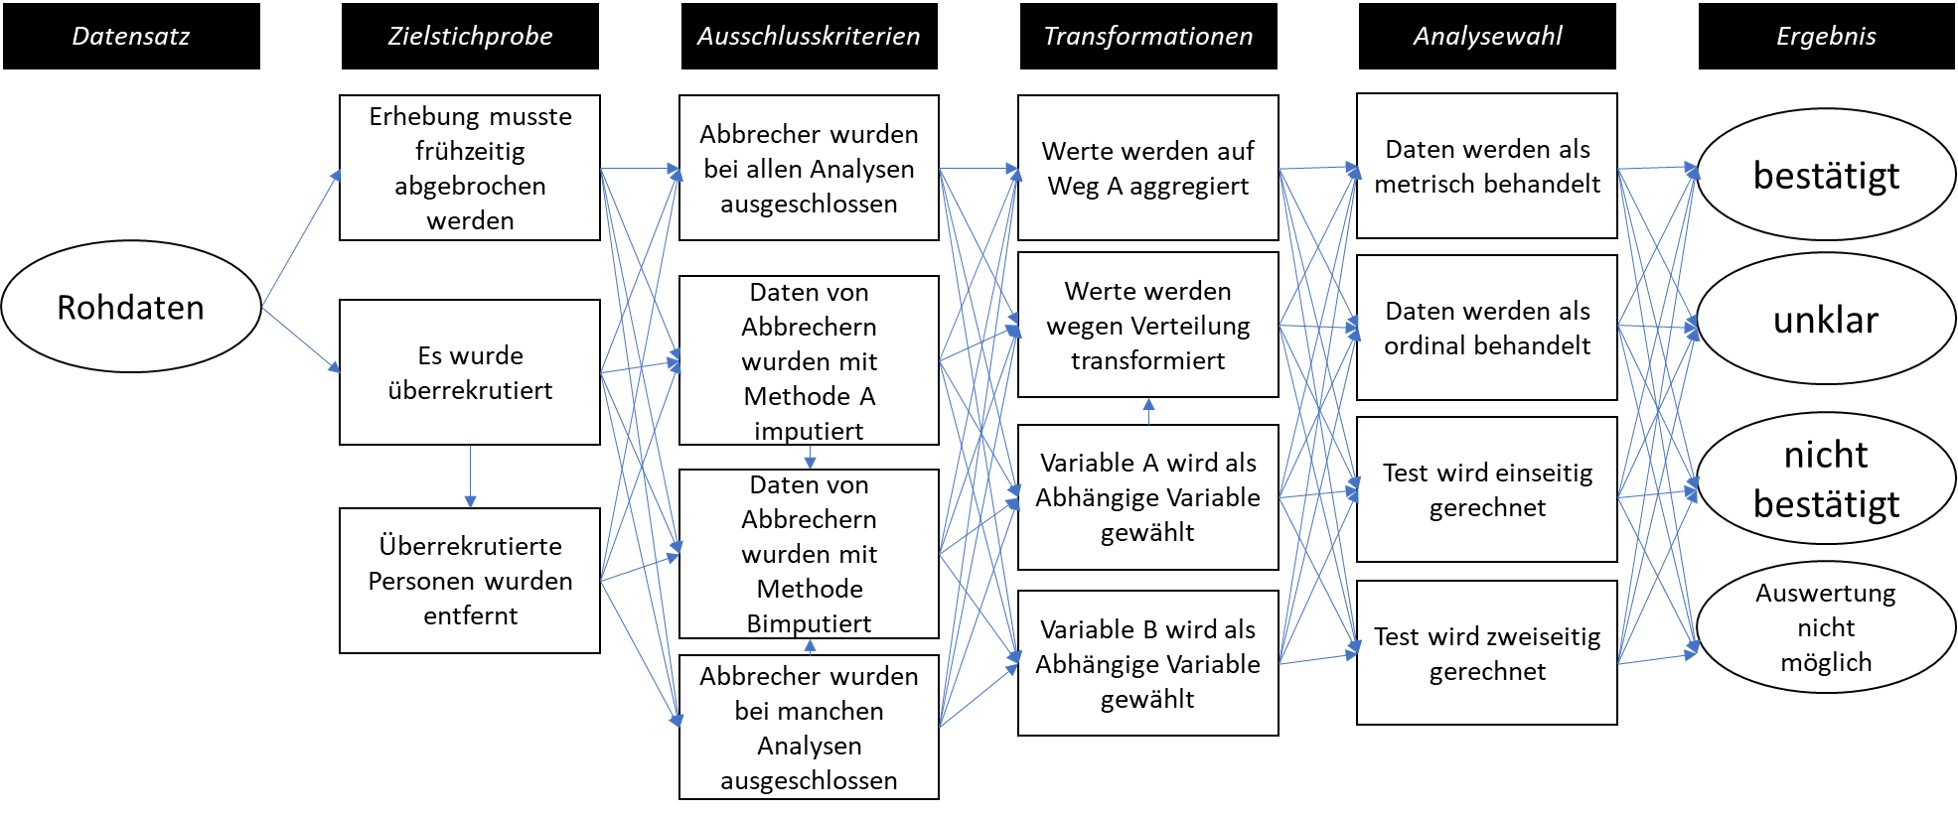
\includegraphics{images/gardenofforkingpaths.jpg}

}

\caption{192 verschiedene Wege von einem Datensatz zum (gewünschten)
Ergebnis}

\end{figure}%

Demonstrationen des \emph{garden of forking paths} existieren für
verschiedenste Felder und wurden bereits für Evolutionsbiologie (Gould
et al. 2023), Sozialpolitik (Breznau et al. 2022),
Strukturgleichungsmodelle (Sarstedt et al. 2024), und Sprachanalysen
(Coretta et al. 2023) nachgewiesen.

\subsection{Tippfehler}\label{tippfehler}

Häufig werden Daten mittels fortgeschrittener Programme ausgewertet und
die Ergebnisse werden dann mühselig in den Bericht übertragen. Hierbei
entstehen schnell Tippfehler. Michèle B. Nuijten et al. (2016)
erstellten einen Algorithmus, der automatisch berichtete
Signifikanztests erkennt, nachrechnet, und Inkonsistenzen zurückmeldet.
Dabei fanden sie heraus, dass in großen Psychologiezeitschriften
zwischen 1985 und 2013 in ungefähr der Hälfte aller Artikel mindestens
ein Fehler war. Diese ``Tippfehler'' waren dabei nicht völlig zufällig,
sondern fehlerhafte Werte waren meistens zugunsten positiver Befunde.
Solche Übertragungsfehler passieren auch bei Meta-Analysen
(Lopez-Nicolas et al. 2022). Und selbst bei Zitationen sind Fehler nicht
selten: Über verschiedene wissenschaftliche Disziplinen fanden (Smith
and Cumberledge 2020), dass in 25\% aller untersuchten Zitationen, die
zitierten Behauptungen in den Originalartikeln nicht vertreten wurden.

\subsection{P-Hacking}\label{p-hacking}

Der P-Wert bei statistischen Tests gibt an, wie hoch die
Wahrscheinlichkeit für das beobachtete Muster ist, gegeben eines
vorausgesetzten Musters. Für eine Korrelation heißt das: Wie
wahrscheinlich ist es, eine Korrelation der vorgefundenen Höhe zu
beobachten, wenn eigentlich kein Zusammenhang (also \emph{r} = 0)
zwischen den untersuchten Variablen besteht. Konkret könnte das heißen:
Wie wahrscheinlich ist es, dass in meinem Datensatz von 100 Personen die
Korrelation zwischen Intelligenz und Alter genau \emph{r}(98) = .420
ist, wenn ich eigentlich davon ausgehen, dass beide Variablen nicht
zusammenhängen.

Die im Signifikanztest mitformulierte Annahme des fehlenden
Zusammenhanges heißt \emph{Nullhypothese}. Wenn das beobachtete Muster
gegeben der Nullhypothese extrem unwahrscheinlich ist (oft unter 5\%)
wird von einem statistisch signifikanten Zusammenhang gesprochen.
Wichtig ist dabei, dass Signifikanz (also „Bedeutsamkeit'') hier
wirklich nur im statistischen Sinne zu verstehen ist. Die Frage, wie
bedeutsam ein Befund für die Welt und das Leben ist, lässt sich mit
Statistik in diesem Rahmen nicht beantworten. Weil P-Werte
Wahrscheinlichkeiten sind, liegen sie zwischen 0 und 100\%.

Unter den QRPs (fragwürdigen Forschungspraktiken) ist p-hacking eine
weitere Kategorie, die wiederum selbst verschiedene Techniken
beinhaltet. Mit p-hacking ist gemeint, dass Forschende ihre
Freiheitsgrade nutzen, um den P-Wert „signifikant zu machen'', also
unter 5\% zu bringen. Eine oft fälschlicherweise gemachte Annahme zu
P-Werten ist, dass hohe P-Werte für die \emph{Abwesenheit} eines
Zusammenhanges sprächen, oder dass P-Werte nur dann niedrig sind, wenn
tatsächlich ein Zusammenhang vorliegt. Stattdessen sind P-Werte
tendenziell klein, wenn ein Zusammenhang vorliegt, der auch mit der
Menge der erhobenen Daten nachgewiesen werden kann. Wenn kein
Zusammenhang vorliegt, sind P-Werte gleichverteilt, das heißt, alle
P-Werte kommen gleich häufig vor. Im Sinne der oben genannten Definition
ist a priori klar, dass bei 100 durchgeführten Studien tendenziell 5
einen signifikanten Zusammenhang aufweisen, \emph{wenn eigentlich keiner
vorliegt}. Diese Tatsache erlaubt diverse P-Hacking Methoden. Simonsohn
et al.~(2014) zeigten, die Wahrscheinlichkeit, ein signifikantes
Ergebnis zu kriegen, wenn eigentlich kein Zusammenhang in den Daten
herrscht, von 5\% auf ca. 60\% steigen kann. Abbildung X zeigt die
Verteilung von P-Werten bei verschieden hoher Teststärke (bzw. Power:
der Wahrscheinlichkeit, einen Zusammenhang einer bestimmten Größe zu
finden, wenn es ihn tatsächlich gibt).

\emph{P-Werte sind bei Abwesenheit von Unterschieden oder
Zusammenhängen, also beim Gelten der Nullhypothese gleichverteilt. Je
höher die statistische Teststärke (Power), desto weiter verschiebt sich
die Verteilung in den Bereich statistischer Signifikanz.}

\begin{Shaded}
\begin{Highlighting}[]
\CommentTok{\# P{-}Value distribution {-}{-}{-}{-}{-}{-}{-}{-}{-}{-}{-}{-}{-}{-}{-}{-}{-}{-}{-}{-}{-}{-}{-}{-}{-}{-}{-}{-}{-}{-}{-}{-}{-}{-}{-}{-}{-}{-}{-}{-}{-}{-}{-}{-}{-}{-}{-}{-}{-}{-}{-}{-} }
\FunctionTok{layout}\NormalTok{(}\FunctionTok{matrix}\NormalTok{(}\FunctionTok{c}\NormalTok{(}\DecValTok{1}\NormalTok{,}\DecValTok{2}\NormalTok{,}\DecValTok{3}\NormalTok{), }\AttributeTok{nrow =} \DecValTok{1}\NormalTok{)) }

\NormalTok{effects }\OtherTok{\textless{}{-}} \FunctionTok{c}\NormalTok{(}\DecValTok{0}\NormalTok{, .}\DecValTok{1}\NormalTok{, .}\DecValTok{3}\NormalTok{) }

\ControlFlowTok{for}\NormalTok{ (i }\ControlFlowTok{in}\NormalTok{ effects) \{ }
\NormalTok{  effect }\OtherTok{\textless{}{-}}\NormalTok{ i }
\NormalTok{  n }\OtherTok{\textless{}{-}} \DecValTok{100} 
\NormalTok{  pvalues }\OtherTok{\textless{}{-}}\NormalTok{ (}\FunctionTok{replicate}\NormalTok{(}\DecValTok{1000}\NormalTok{, }\FunctionTok{t.test}\NormalTok{(}\FunctionTok{rnorm}\NormalTok{(}\DecValTok{100}\NormalTok{), }\FunctionTok{rnorm}\NormalTok{(}\DecValTok{100}\NormalTok{, i))}\SpecialCharTok{$}\NormalTok{p.value)) }
\NormalTok{  power }\OtherTok{\textless{}{-}} \FunctionTok{round}\NormalTok{(pwr}\SpecialCharTok{::}\FunctionTok{pwr.t.test}\NormalTok{(}\AttributeTok{n =}\NormalTok{ n, }\AttributeTok{d =}\NormalTok{ i, }\AttributeTok{power =} \ConstantTok{NULL}\NormalTok{, }\AttributeTok{alternative =} \StringTok{"two.sided"}\NormalTok{)}\SpecialCharTok{$}\NormalTok{power, }\DecValTok{3}\NormalTok{) }
  
  \FunctionTok{hist}\NormalTok{(pvalues}
\NormalTok{       , }\AttributeTok{xlab =} \StringTok{"P{-}Werte"}
\NormalTok{       , }\AttributeTok{ylab =} \StringTok{"Anzahl"}
\NormalTok{       , }\AttributeTok{main =} \FunctionTok{paste}\NormalTok{(}\StringTok{"Effektstärke d = "}\NormalTok{, i, }\StringTok{"}\SpecialCharTok{\textbackslash{}n}\StringTok{Power = "}\NormalTok{, power, }\AttributeTok{sep =} \StringTok{""}\NormalTok{) }
\NormalTok{       , }\AttributeTok{xlim =} \FunctionTok{c}\NormalTok{(}\DecValTok{0}\NormalTok{, }\DecValTok{1}\NormalTok{)}
\NormalTok{       , }\AttributeTok{yaxt =} \StringTok{\textquotesingle{}n\textquotesingle{}}\NormalTok{) }
\NormalTok{  \} }
\end{Highlighting}
\end{Shaded}

\includegraphics{probleme_methoden_files/figure-pdf/unnamed-chunk-3-1.pdf}

\begin{Shaded}
\begin{Highlighting}[]
\FunctionTok{layout}\NormalTok{(}\DecValTok{1}\NormalTok{)}
\end{Highlighting}
\end{Shaded}

Die Chance, signifikante P-Werte zu kriegen, ohne, dass die getestete
Hypothese überhaupt stimmt, lässt sich durch „zerschneiden'' der
Stichprobe machen (z.B. werden nur Frauen analysiert), durch das Erheben
zusätzlicher Daten („optional stopping''), oder durch die Verwendung
mehrerer zentraler Variablen (zum Beispiel wird Intelligenz mit 3
verschiedenen Tests erfasst und alle werden einzeln mit Alter
korreliert). Selbst das verändern kleiner Parameter in den statistischen
Tests (z.B. Verwendung einer nicht-parametrischen Spearman Korrelation
statt der Bravais-Pearson Korrelation) erhöhen die Chancen auf ein
signifikantes Ergebnis (siehe Tabelle Y). Einige Formen des
\emph{p-hacking} lassen sich zum Beispiel hier ausprobieren:
\url{https://shinyapps.org/apps/p-hacker/} (Schönbrodt 2016). Eine
Checkliste, um P-Hacking zu vermeiden, schlägt Wicherts et al. (2016)
vor.

\emph{Wahrscheinlichkeit für ein signifikantes Ergebnis durch die
Anwendung verschiedener P-Hacking Techniken nach Simmons, Nelson, and
Simonsohn (2011), Tabelle 1. Der Anteil signifikanter Ergebnisse sollte
hier den festgelegten 5\% des Alpha-Fehlers entsprechen.}

\begin{longtable}[]{@{}
  >{\raggedright\arraybackslash}p{(\columnwidth - 2\tabcolsep) * \real{0.6667}}
  >{\raggedright\arraybackslash}p{(\columnwidth - 2\tabcolsep) * \real{0.3333}}@{}}
\toprule\noalign{}
\begin{minipage}[b]{\linewidth}\raggedright
Technik
\end{minipage} & \begin{minipage}[b]{\linewidth}\raggedright
Anteil signifikanter Ergebnisse
\end{minipage} \\
\midrule\noalign{}
\endhead
\bottomrule\noalign{}
\endlastfoot
Mehrere abhängige Variablen, deren Korrelation r = .5 ist & 9,5\% \\
10 weitere Beobachtungen je Gruppe erheben & 7,7\% \\
Eine weitere Variable (z.B. Geschlecht) mit in das Modell aufnehmen &
11,7\% \\
Ausschließen (bzw. Beibehalten) einer von drei Gruppen & 12,6\% \\
Alle Techniken gleichzeitig & 60,7\% \\
\end{longtable}

\begin{tcolorbox}[enhanced jigsaw, title=\textcolor{quarto-callout-tip-color}{\faLightbulb}\hspace{0.5em}{Forschung kann nicht witzig sein?}, colbacktitle=quarto-callout-tip-color!10!white, rightrule=.15mm, titlerule=0mm, left=2mm, bottomrule=.15mm, arc=.35mm, leftrule=.75mm, toprule=.15mm, opacityback=0, breakable, bottomtitle=1mm, colframe=quarto-callout-tip-color-frame, toptitle=1mm, opacitybacktitle=0.6, coltitle=black, colback=white]

Hussey and Hughes (2018) (und darauf aufbauend Sarstedt and Adler
(2023)) schlugen bereits Methoden vor, um P-Hacking noch stärker zu
erleichtern. Auf dieser Website können Benutzer*innen Zufallszahlen in
dem gewünschten Bereich generieren:
\url{https://mktg.shinyapps.io/extra-p_ointless/}

\end{tcolorbox}

\subsection{\texorpdfstring{Selektives Berichten (\emph{Selective
Reporting})}{Selektives Berichten (Selective Reporting)}}\label{selektives-berichten-selective-reporting}

Im Rahmen der Planung einer sozialwissenschaftlichen Studie stellt sich
oft die Frage, wie ein bestimmtes Konstrukt gemessen werden soll. Für
Intelligenz, politischer Ansicht, Lebenszufriedenheit, und viele andere
Variable gibt es nicht \emph{den} Test sondern viele Maße, die teilweise
gering miteinander zusammenhängen. Gleichzeitig sind die zu testenden
Theorien meist vage und diktieren nicht, mit welchem Maß ein Konstrukt
gemessen werden sollte. Theorien sind den Messmethoden gegenüber also
oft agnostisch. Werden in einer Studie dann verschiedene Messmethoden
für ein Konstrukt gewählt, müsste die Theorie über alle Tests
gleichermaßen bestätigt werden. Falls das nicht der Fall ist, sollte die
Theorie angepasst werden. Entgegen dieser Empfehlung und um die Chance
der Publikation der Ergebnisse zu maximieren, berichten Forschende
Ergebnisse oft \emph{selektiv}. Statt aller Ergebnisse werden also nur
die „passendsten'' oder „spannendsten'' berichtet. Wie oben im Thema
P-Hacking und Freiheitsgrade von Forschenden klar geworden ist, führt
das dazu, dass Zusammenhänge gefunden werden, die eigentlich nicht
existieren. Werden zum Beispiel drei verschiedene und unabhängige Maße
zum Testen einer Hypothese verwendet steigt Wahrscheinlichkeit für
mindestens ein signifikantes Ergebnis von 5\% auf 14\%.

\textbf{Abbildung K}

Selektives Berichten: Von den sechs geprüften Korrelationen ist nur eine
signifikant - und das rein zufällig. Alle gemeinsam sind nicht
signifikant. Um die Ergebnisse zu veröffentlichen berichten Forschende
nur den spannendsten Teil der Ergebnisse und verzerren damit das Bild.
Die Chance, aus sechs Tests - bei denen keine Zusammenhänge vorliegen -
einen signifikanten zu erhalten liegt bei ca. 27\%.

\begin{Shaded}
\begin{Highlighting}[]
\CommentTok{\# mean(replicate(1000, mean(replicate(6, cor.test(rnorm(50), rnorm(50))$p.value) \textless{} .05) \textgreater{} 0)) \# 26.7\%}
\FunctionTok{set.seed}\NormalTok{(}\DecValTok{1}\NormalTok{)}
\NormalTok{n }\OtherTok{\textless{}{-}} \DecValTok{100}

\FunctionTok{layout}\NormalTok{(}\FunctionTok{matrix}\NormalTok{(}\FunctionTok{c}\NormalTok{(}\DecValTok{1}\SpecialCharTok{:}\DecValTok{6}\NormalTok{), }\AttributeTok{nrow =} \DecValTok{2}\NormalTok{)) }
\ControlFlowTok{for}\NormalTok{ (i }\ControlFlowTok{in} \DecValTok{1}\SpecialCharTok{:}\DecValTok{6}\NormalTok{) \{}
\NormalTok{  x }\OtherTok{\textless{}{-}} \FunctionTok{rnorm}\NormalTok{(n)}
\NormalTok{  y }\OtherTok{\textless{}{-}} \FunctionTok{rnorm}\NormalTok{(n)}
  
  \FunctionTok{plot}\NormalTok{(x, y}
\NormalTok{       , }\AttributeTok{main =} \FunctionTok{paste}\NormalTok{(}\StringTok{"r("}\NormalTok{, n}\DecValTok{{-}2}\NormalTok{, }\StringTok{") = "}\NormalTok{, }\FunctionTok{round}\NormalTok{(}\FunctionTok{cor}\NormalTok{(x,y), }\DecValTok{3}\NormalTok{), }\StringTok{", p = "}\NormalTok{, }\FunctionTok{round}\NormalTok{((}\FunctionTok{cor.test}\NormalTok{(x,y)}\SpecialCharTok{$}\NormalTok{p.value), }\DecValTok{3}\NormalTok{), }\AttributeTok{sep =} \StringTok{""}\NormalTok{)}
\NormalTok{       , }\AttributeTok{pch =} \DecValTok{20}\NormalTok{, }\AttributeTok{yaxt =} \StringTok{\textquotesingle{}n\textquotesingle{}}\NormalTok{, }\AttributeTok{xaxt =} \StringTok{\textquotesingle{}n\textquotesingle{}}\NormalTok{, }\AttributeTok{xlab =} \StringTok{""}\NormalTok{, }\AttributeTok{ylab =} \StringTok{""}\NormalTok{)}
\NormalTok{\}}
\end{Highlighting}
\end{Shaded}

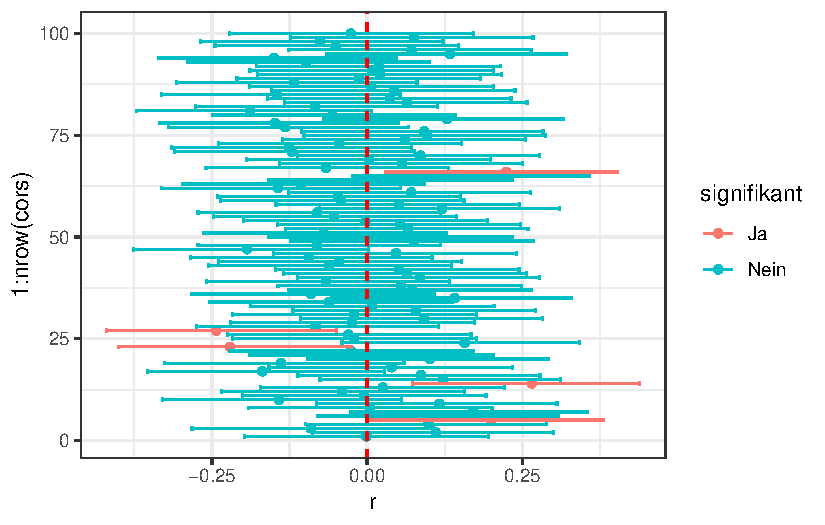
\includegraphics{probleme_methoden_files/figure-pdf/unnamed-chunk-4-1.pdf}

\begin{Shaded}
\begin{Highlighting}[]
\FunctionTok{layout}\NormalTok{(}\DecValTok{1}\NormalTok{)}
\end{Highlighting}
\end{Shaded}

\subsection{Optionales Stoppen (Optional
Stopping)}\label{optionales-stoppen-optional-stopping}

Führt man bei der Durchführung einer Studie nach jeder Beobachtung den
Test erneut aus und betrachtet den P-Wert, dann gibt es zwei
Möglichkeiten zum Verlauf der P-Werte: Falls ein Zusammenhang zwischen
den erhobenen Variablen besteht, wird der P-Wert \emph{konvergieren},
also sich einem bestimmten Wert annähern, nämlich 0. Die
Wahrscheinlichkeit für das beobachtete Ergebnis wird mit größerer
Stichprobe immer geringer. Dass eine Münze nur auf ``Kopf'' landet ist
ungewöhnlicher, wenn sie das 100 Mal getan hat, als wenn sie das 3 Mal
tat. Falls kein Zusammenhang vorliegt, wird der P-Wert nicht wie oft
erwartet gegen 1 gehen, sondern \emph{nicht konvergieren}. Er wird dann
chaotisch mal hoch und mal niedrig sein -- und auch öfter mal
signifikant. Diese Tatsache machen sich Forschende beim optionalen
Stoppen zu Nutzen: Sie erheben so lange Daten, bis ihre Hypothese
bestätigt wird. Das Problem besteht übrigens nicht für Effektstärkemaße
wie zum Beispiel Korrelationen. Diese konvergieren je nach Größe ab
ungefähr 250 Beobachtungen (Schönbrodt \& Perugini, 2013).

\textbf{Abbildung P}

\emph{Konvergenz von P-Werten und Effektstärken je nach Effektgröße:
Effektstärken (hier: Korrelationskoeffizienten) konvergieren bei großen
Stichproben, P-Werte konvergieren nur, wenn die Korrelation nicht 0
ist.}

\begin{Shaded}
\begin{Highlighting}[]
\CommentTok{\# P{-}Value Convergence {-}{-}{-}{-}{-}{-}{-}{-}{-}{-}{-}{-}{-}{-}{-}{-}{-}{-}{-}{-}{-}{-}{-}{-}{-}{-}{-}{-}{-}{-}{-}{-}{-}{-}{-}{-}{-}{-}{-}{-}{-}{-}{-}{-}{-}{-}{-}{-}{-}{-}{-}{-}{-} }
\NormalTok{imax }\OtherTok{\textless{}{-}} \FunctionTok{seq}\NormalTok{(}\DecValTok{5}\NormalTok{, }\DecValTok{1000}\NormalTok{, }\DecValTok{10}\NormalTok{) }
\NormalTok{p0 }\OtherTok{\textless{}{-}} \ConstantTok{NULL} 
\NormalTok{p1 }\OtherTok{\textless{}{-}} \ConstantTok{NULL} 
\NormalTok{p2 }\OtherTok{\textless{}{-}} \ConstantTok{NULL} 

\ControlFlowTok{for}\NormalTok{ (i }\ControlFlowTok{in}\NormalTok{ imax) \{ }
  
  \FunctionTok{set.seed}\NormalTok{(}\DecValTok{42}\NormalTok{) }
  
\NormalTok{  ds0 }\OtherTok{\textless{}{-}}\NormalTok{ MASS}\SpecialCharTok{::}\FunctionTok{mvrnorm}\NormalTok{(}\AttributeTok{n =}\NormalTok{ i, }\AttributeTok{mu =} \FunctionTok{c}\NormalTok{(}\DecValTok{0}\NormalTok{,}\DecValTok{0}\NormalTok{), }\AttributeTok{Sigma =} \FunctionTok{matrix}\NormalTok{(}\FunctionTok{c}\NormalTok{(}\DecValTok{1}\NormalTok{, }\DecValTok{0}\NormalTok{, }\DecValTok{0}\NormalTok{, }\DecValTok{1}\NormalTok{), }\AttributeTok{nrow =} \DecValTok{2}\NormalTok{)) }
\NormalTok{  ds1 }\OtherTok{\textless{}{-}}\NormalTok{ MASS}\SpecialCharTok{::}\FunctionTok{mvrnorm}\NormalTok{(}\AttributeTok{n =}\NormalTok{ i, }\AttributeTok{mu =} \FunctionTok{c}\NormalTok{(}\DecValTok{0}\NormalTok{,}\DecValTok{0}\NormalTok{), }\AttributeTok{Sigma =} \FunctionTok{matrix}\NormalTok{(}\FunctionTok{c}\NormalTok{(}\DecValTok{1}\NormalTok{, .}\DecValTok{05}\NormalTok{, .}\DecValTok{05}\NormalTok{, }\DecValTok{1}\NormalTok{), }\AttributeTok{nrow =} \DecValTok{2}\NormalTok{)) }
\NormalTok{  ds2 }\OtherTok{\textless{}{-}}\NormalTok{ MASS}\SpecialCharTok{::}\FunctionTok{mvrnorm}\NormalTok{(}\AttributeTok{n =}\NormalTok{ i, }\AttributeTok{mu =} \FunctionTok{c}\NormalTok{(}\DecValTok{0}\NormalTok{,}\DecValTok{0}\NormalTok{), }\AttributeTok{Sigma =} \FunctionTok{matrix}\NormalTok{(}\FunctionTok{c}\NormalTok{(}\DecValTok{1}\NormalTok{, .}\DecValTok{1}\NormalTok{, .}\DecValTok{1}\NormalTok{, }\DecValTok{1}\NormalTok{), }\AttributeTok{nrow =} \DecValTok{2}\NormalTok{)) }
  
\NormalTok{  p0 }\OtherTok{\textless{}{-}} \FunctionTok{c}\NormalTok{(p0, }\FunctionTok{cor.test}\NormalTok{(ds0[, }\DecValTok{1}\NormalTok{], ds0[, }\DecValTok{2}\NormalTok{])}\SpecialCharTok{$}\NormalTok{p.value) }
\NormalTok{  p1 }\OtherTok{\textless{}{-}} \FunctionTok{c}\NormalTok{(p1, }\FunctionTok{cor.test}\NormalTok{(ds1[, }\DecValTok{1}\NormalTok{], ds1[, }\DecValTok{2}\NormalTok{])}\SpecialCharTok{$}\NormalTok{p.value) }
\NormalTok{  p2 }\OtherTok{\textless{}{-}} \FunctionTok{c}\NormalTok{(p2, }\FunctionTok{cor.test}\NormalTok{(ds2[, }\DecValTok{1}\NormalTok{], ds2[, }\DecValTok{2}\NormalTok{])}\SpecialCharTok{$}\NormalTok{p.value) }
  
\NormalTok{\} }

\FunctionTok{plot}\NormalTok{( }\AttributeTok{y =}\NormalTok{ p0, }\AttributeTok{x =}\NormalTok{ imax, }\AttributeTok{type =} \StringTok{"l"}\NormalTok{, }\AttributeTok{col =} \StringTok{"grey"}\NormalTok{, }\AttributeTok{xlab =} \StringTok{"Stichprobengröße (Anzahl der Beobachtungen)"}\NormalTok{, }\AttributeTok{ylab =} \StringTok{"P{-}Wert"}\NormalTok{) }
\FunctionTok{lines}\NormalTok{(}\AttributeTok{y =}\NormalTok{ p1, }\AttributeTok{x =}\NormalTok{ imax, }\AttributeTok{col =} \StringTok{"orange"}\NormalTok{) }
\FunctionTok{lines}\NormalTok{(}\AttributeTok{y =}\NormalTok{ p2, }\AttributeTok{x =}\NormalTok{ imax, }\AttributeTok{col =} \StringTok{"red"}\NormalTok{) }
\FunctionTok{abline}\NormalTok{(}\AttributeTok{h =}\NormalTok{ .}\DecValTok{05}\NormalTok{, }\AttributeTok{lty =} \DecValTok{2}\NormalTok{)}
\FunctionTok{legend}\NormalTok{(}\StringTok{"topright"}\NormalTok{, }\FunctionTok{c}\NormalTok{(}\StringTok{"r = 0"}\NormalTok{, }\StringTok{"r = .05"}\NormalTok{, }\StringTok{"r = .1"}\NormalTok{), }\AttributeTok{col =} \FunctionTok{c}\NormalTok{(}\StringTok{"grey"}\NormalTok{, }\StringTok{"orange"}\NormalTok{, }\StringTok{"red"}\NormalTok{), }\AttributeTok{lty =} \DecValTok{1}\NormalTok{)}
\end{Highlighting}
\end{Shaded}

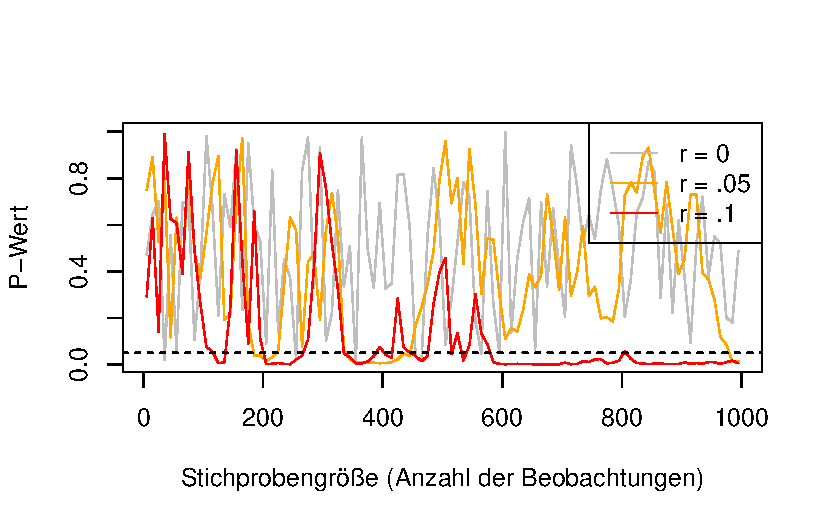
\includegraphics{probleme_methoden_files/figure-pdf/unnamed-chunk-5-1.pdf}

\subsection{\texorpdfstring{Darstellung kalibrierter Modelle als
geplante Modelle
(\emph{Overfitting})}{Darstellung kalibrierter Modelle als geplante Modelle (Overfitting)}}\label{darstellung-kalibrierter-modelle-als-geplante-modelle-overfitting}

Komplexe statistische Modelle haben viele Stellschrauben. Es ist
möglich, die unzähligen Entscheidungen vor Anwendung eines Modells auf
Daten zu treffen, für gewöhnlich werden aber andere Kalibrationen
ausprobiert und eine andere als die geplante hat eine bessere Passung.
Damit ist gemeint, dass beispielsweise bestimmte Variablen mit in ein
Modell aufgenommen werden, um die Vorhersagekraft zu maximieren. Zu
vielen Modellen gehören sogar verschiedene Algorithmen, die auf Basis
festgelegter Regeln entscheiden, wie das Modell aussehen soll. Ein
Modell wird also an ein Datenmuster angepasst. Wird das Vorgehen
transparent offengelegt, ist das absolut in Ordnung. Problematisch wird
es, wenn das beste gefundene Modell als geplantes Modell dargestellt
wird. Das in den Daten vorliegende Muster beinhaltet in
sozialwissenschaftlichen Untersuchungen nämlich fast immer auch ein
Rauschen, also Schwankungen, die auf Messungenauigkeiten oder andere
unbekannte Einflüsse zurückzuführen sind. Diese Einflüsse schwanken
definitionsgemäß (in der psychologischen Testtheorie ist zum Beispiel
die Rede vom \emph{Error}, einer unsystematischen Schwankung, die sich
bei häufiger Messung herausmittelt). Bei zukünftigen Untersuchen wird
das an die vergangenen Daten und das darin enthaltene Rauschen
angepasste Modell dann notwendigerweise schlechter abschneiden, weil das
Rauschen in den neuen Daten ein anderes ist. Man spricht dann von einem
„überangepassten'' Modell oder Overfitting.

\subsection{\texorpdfstring{Tendenz von Menschen, sich selbst zu
bestätigen (\emph{Confirmation
Bias})}{Tendenz von Menschen, sich selbst zu bestätigen (Confirmation Bias)}}\label{tendenz-von-menschen-sich-selbst-zu-bestuxe4tigen-confirmation-bias}

Ein besonderes Problem wissenschaftlicher Methoden ist der Confirmation
Bias. Das Phänomen ist in der wissenschaftlichen Literatur nicht klar
definiert (Nickerson 1998), hier meine ich damit die Tendenz von
Menschen (oder in diesem Kontext: Forschenden), diejenigen Muster zu
finden, die sie erwarten. Der Confirmation Bias basiert auf
wissenschaftlichen Befunden (Oswald and Grosjean 2004) und wurde von den
Wissenschaftler*innen auf sie selbst übertragen (Mynatt, Doherty, and
Tweney 1977; Yu et al. 2014). Diese Gedanken führen nah an logischen
Unsinnigkeiten und Paradoxa entlang, selbstironisch bemerkt zum Beispiel
Nickerson (1998) die Möglichkeit, dass alle Befunde zu Confirmation
Biases selbst nur Produkte desselben sein könnten, was die Existenz des
Confirmation Biases dann wieder bestätigen würde (S. 211). Praktisch
besteht die Gefahr, dass Wissenschaftler*innen nicht Wahrheiten
herausfinden, sondern alles so drehen, dass ihre Vorahnungen bestätigt
werden. Ludwik Fleck (1935/2015) geht in seiner Wissenschaftssoziologie,
die die Grundlage für Thomas Kuhns Arbeit zu wissenschaftlichen
Revolutionen (Kuhn 1970/1996) bildet, noch ein paar Schritte weiter: Er
argumentiert für ein Modell des wissenschaftlichen Fortschritts, bei dem
es nicht darum geht, der Wahrheit näher zu kommen, sondern nach bestem
Wissen Probleme vor dem gesellschaftlichen Hintergrund zu verstehen. Das
heißt nicht, dass es keine Wahrheit gibt, nur dass Wahrheit eben nicht
bloß die Übereinstimmung von Aussagen mit Tatsachen ist. Statt dieser
oft von Wissenschaftler*innen vertretenen \emph{Korrespondenztheorie von
Wahrheit}, findet sich bei Fleck eine \emph{Konsenstheorie} von Wahrheit
wieder: Die Übereinstimmung vieler Leute ist wichtig. Wissenschaftliche
Tatsachen werden nicht von einzelnen Personen „entdeckt'', sondern von
einem Kollektiv erschaffen. Der Confirmation Bias findet sich dabei so
wieder, dass dem Konsens widersprechende Befunde ausgeblendet werden und
auf den aktuellen Auffassungen so lange wie möglich beharrt wird.
Wenngleich philosophische Wahrheitstheorien den Rahmen dieses Buches
sprengen, sei darauf hingewiesen, dass keine der drei Wahrheitstheorien
(Korrespondenz, Konsens, und Kohärenz) haltbar ist {[}Albert (2010);
\emph{Münchhausen Trilemma}{]}.

\subsection{Datenfälschung}\label{datenfuxe4lschung}

Die bisher diskutierten Praktiken werden oft als fragwürdig
(questionable) dargestellt. Manche Wissenschaftler*innen halten das für
ein Euphemismus, denn in der Verantwortung als Forscher*in sollte
genügend Wissen vorliegen, um zu erkennen, dass die oben beschriebenen
Techniken \emph{nicht} wissenschaftlich sind und eindeutig nicht der
Generierung von Wissen dienen. Sie behindern deutlich den
wissenschaftlichen Fortschritt, gefährden das Vertrauen in Wissenschaft,
und führen zu enorm hohen Kosten. Unglücklicherweise sind diese
Problematiken vielen Wissenschaftler*innen heute immer noch nicht
bekannt. „Das haben wir halt so gelernt und schon immer so gemacht''
heißt es zum Beispiel. Dass bestimmte Studien sich nicht replizieren
ließen, war teilweise schon vielen Personen bewusst, sie hielten es nur
nicht für möglich, das im Scientific Record festzuhalten. Jedenfalls
legt der Begriff der fragwürdigen Forschungspraktiken nahe, dass sich
Forschende damit in einer Grauzone bewegen würden. Meiner Ansicht nach,
ist das nur der Fall, da, wenn Forschende ihren Job verlieren würden,
weil sie P-Hacking betrieben haben, nicht mehr viele Forschende übrig
wären.

Anders ist es beim Fälschen und Manipulieren von Daten. Wie häufig
Datenmanipulationen oder -fälschungen vorkommen ist ungewiss und
Schätzungen sind schwierig. In einer Meta-Analyse von Umfragen zu dem
Thema wurde geschätzt, dass zwischen 0,86 und 4,45\% aller
Wissenschaftler*innen zugaben, Daten manipuliert zu haben. 72\% gaben
an, fragwürdige Forschungspraktiken anzuwenden (Fanelli 2009). Stroebe,
Postmes, and Spears (2012) stellten später Beispiele von Datenfälschung
zusammen und empfahlen Peer Review und Replikationen als
Betrugs-Detektoren. Eine neuere und extrem umfangreiche Studie von
Gopalakrishna, Wicherts, et al. (2021) berichtete, dass 8,3\% aller
Befragten Daten manipuliert oder gefälscht hätten und 51,3\% fragwürdige
Forschungspraktiken angewandt hätten (Tabelle 2) und bestätigte den
Ausmaß der Probleme. Je nach Disziplinen kommen weitere Probleme hinzu,
wie zum Beispiel die Verwendung bereits veröffentlichter
biomedizinischer Bilder, die in ungefähr 3,8\% aller veröffentlichten
Artikel angewandt wurde (Bik, Casadevall, and Fang 2016). Es wird davon
ausgegangen, dass Datenfälschung nur in sehr seltenen Fällen aufgedeckt
wird. Diejenigen Fälle, die ans Licht kamen, hatten die Zurückziehung
(\emph{Retraction}) der jeweiligen wissenschaftlichen Artikel zur Folge
und oft Konsequenzen für die wissenschaftliche Karriere der
Verantwortlichen. Retractionwatch.org verwaltet die weltweit größte
Datenbank zu zurückgezogenen Artikeln (Stand Dezember 2023: 49.628
Artikel): \url{http://retractiondatabase.org/}.

Sehr düster ist dabei die Tatsache, dass Methoden zur Datenfälschung
einerseits immer einfacher werden (Naddaf 2023) und
Wissenschaftler*innen, die Fehler aufdecken, gelegentlich verklagt
werden. Das betrifft beispielsweise wurden die Autoren von
Datacolada.org, die bereits häufiger Probleme aufgezeigt haben, von
Francesca Gino für die Veröffentlichung verklagt
(\url{https://datacolada.org/109}), woraufhin tausende
Wissenschaftler*innen Gelder für die finanzielle Unterstützung des
Gerichtsprozesses sammelten
(\url{https://www.gofundme.com/f/uhbka-support-data-coladas-legal-defense}).

\section{Weiterführende
Informationen}\label{weiterfuxfchrende-informationen}

\begin{itemize}
\tightlist
\item
  Bei diesem englischsprachigen Podcast wird diskutiert, wie und ob sich
  Betrug in der Wissenschaft stoppen lässt:
  \url{https://freakonomics.com/podcast/can-academic-fraud-be-stopped/}
\item
  Wie sich die Replikationskrise aus Perspektive eines jungen Forschers
  angefühlt hat beschreibt Daniel Lakens:
  \url{http://daniellakens.blogspot.com/2020/11/why-i-care-about-replication-studies.html}
\end{itemize}

\subsection{Literatur}\label{literatur-10}

\chapter{Theorien}\label{theorien}

Wissenschaft arbeitet mit Theorien. Wie diese genau aussehen,
unterscheidet sich zwischen Disziplinen deutlich. Während
naturwissenschaftliche Bereiche häufig mit mathematischen Modellen, also
Formeln, arbeiten, die den Zusammenhang zwischen Variablen explizit und
unmissverständlich beschreiben und Vorhersagen erlauben, arbeiten
Sozialwissenschaften häufig mit verbalen Theorien im Stile von „X und Y
hängen positiv miteinander zusammen'' oder „je höher X, desto höher Y''
und traditionelle Geisteswissenschaften arbeiten beispielsweise mit
verbalen Erklärungen. Verbale Theorien haben den Vorteil, dass sie
tendenziell leicht verständlich und allgemein anwendbar sind, allerdings
unterliegen die verwendeten Begriffe häufig individuellen, kulturellen,
oder zeitlichen Einflüssen und Diskutant*innen droht, im
wissenschaftlichen Diskurs aneinander vorbei zu reden. Für formale
Theorien werden alle beteiligten Variablen genau definiert und die
Theorien haben häufig einen stark eingeschränkten Geltungsbereich (z.B.
gelten viele physikalische Gesetze nur unter streng kontrollierten
Bedingungen wie im Vakuum, bei einer bestimmten Temperatur, usw.). Die
Sorge im Rahmen der Replikationskrise ist, dass Theorien nicht klar
genug sind, um vorherzusagen, wann Replikationen erfolgreich sind und
damit eine der Ursachen für geringe Replikationsraten sind (Buzbas and
Devezer 2023; P. Smaldino 2019). Eine Theorie über die Konsequenzen von
der Identifikation mit Geschlechterrollen muss beispielsweise die
Veränderung von Geschlechterrollen und Besonderheiten von
Geschlechterrollen in verschiedenen Ländern berücksichtigen. Dass ein
und dasselbe Experiment zu diesem Thema in den USA im Jahre 1980 andere
Ergebnisse hat als in Deutschland im Jahr 2020 ist wenig überraschend.
Problematisch ist allerdings, dass -- auch wenn solche Ergänzungen für
viele sozialwissenschaftliche Theorien sinnvoll und nötig erscheinen --
nur selten Aussagen darüber gemacht werden.

Verbale Theorien sind per se nicht weniger wissenschaftlich: Im Kontext
der jeweiligen Bereiche heben sich wissenschaftliche Theorien stets
durch ihren besonders hohen Grad an Systematizität (Hoyningen-Huene and
Kincaid 2023) von alltagswissenschaftlichen Erklärungen ab. Bereiche,
die Wert auf Vorhersage von Geschehnissen legen, kommen jedoch nicht
ohne formale Theorien aus (Muthukrishna and Henrich 2019). Dabei sei
hervorgehoben, dass bestimmte Wissenschaften eben \emph{keinen Wert} auf
Vorhersage legen (z.B. Geschichtswissenschaften oder Disziplinen, die
vorwiegend hermeneutisch vorgehen). Sozialwissenschaften wie die
Psychologie, quantitative Soziologie, oder Teile der
Geisteswissenschaften („Digital Humanities'') nähern sich aktuell
formalen Modellen an -- in der Sozialpsychologie gab es den Aufruf,
Theorien zu formalisieren beispielsweise schon einmal bei einer Krise in
den 1970er Jahren (Daniel Lakens 2023). Dadurch, dass sich Theorien
durch ihren Mangel an Objektivität selten von verschiedenen Forschenden
verwendet werden und sich durch ihre flexible Auslegung nur schwer
wiederlegen lassen ist dort eine enorm große Menge an nutzlosen Theorien
entstanden (C. J. Ferguson and Heene 2012). Darunter sind auch einander
widersprechende Theorien: Beispielsweise argumentierten Banker et al.
(2017), dass „ego depletion'', also die Erschöpfung von
Selbstkontrollressourcen, dazu führt, dass Personen sich eher an
Hinweise anderer Leute orientieren (S. 2) während Francis et al. (2018)
gegenteilig vermuteten, dass die Erschöpfung verhindert, dass Hinweise
überhaupt verarbeitet werden können. Beide lieferten Daten, die die
jeweiligen Theorien bestätigten, jedoch fand eine Folgeuntersuchung,
dass vermutlich beide falsch lagen (Röseler, Schütz, et al. 2020).

Robinaugh et al. (2021) diskutieren Beispiele der Umwandlung verbaler
Theorien in formale. Dieser Prozess hat zur Folge, dass sich neue und
spezifischere Vorhersagen ableiten lassen. Wenn eine Theorie genauere
Vorhersagen macht und die Menge an möglichen Ereignissen, die der
Theorie widersprechen, steigt, bedeutet das einen gestiegenen
\emph{empirischen Gehalt} (Glöckner and Betsch 2011; Popper 1959/2008).

\begin{tcolorbox}[enhanced jigsaw, title=\textcolor{quarto-callout-tip-color}{\faLightbulb}\hspace{0.5em}{Empirischer Gehalt und Strong Inference}, colbacktitle=quarto-callout-tip-color!10!white, rightrule=.15mm, titlerule=0mm, left=2mm, bottomrule=.15mm, arc=.35mm, leftrule=.75mm, toprule=.15mm, opacityback=0, breakable, bottomtitle=1mm, colframe=quarto-callout-tip-color-frame, toptitle=1mm, opacitybacktitle=0.6, coltitle=black, colback=white]

Theorien können sich in ihrem empirischen Gehalt unterscheiden. Damit
ist konkret gemeint, wie spezifisch ihre Vorhersagen sind. Je mehr
\emph{mögliche} Beobachtungen eine Theorie widerlegen \emph{würden},
desto höher ist ihr empirische Gehalt.

Nehmen wir den Fall, dass unsere Theorie uns erlaubt, Vorhersagen
darüber zu machen, was für ein Auto zu einer bestimmten Zeit an einer
bestimmten Straße entlang fährt. In Abbildung sind alle möglichen Autos
abgebildet. Zur Vereinfachung gibt es in unserer Beispielwelt nur 9
verschiedene Autos, die sich hinsichtlich der Merkmale \emph{Farbe}
(grün, schwarz, blau), \emph{Heckflügel} (mit, ohne), und
\emph{Radfarbe} (grau, gelb) unterscheiden.

\begin{itemize}
\item
  Die lila Theorie sagt: \emph{Das beobachtete Auto hat graue Räder}.
  Ohne Theorie wären für uns alle Autos gleich wahrscheinlich, die lila
  Theorie ``verbietet'', dass das Auto gelbe Räder hat. Sie verbietet
  3/9 Autos.
\item
  Die rote Theorie sagt: \emph{Das beobachtete Auto ist blau}. Die
  Wahrscheinlichkeit, sie zu widerlegen wäre in unserer Musterwelt
  höher, nämlich 6/9. Weil die rote Theorie \emph{a priori}, also ohne
  weiteres Vorwissen, sozusagen eine riskantere Wette ist, hat sie
  höheren empirischen Gehalt.
\item
  Den höchstmöglichen empirischen Gehalt hat die orangene Theorie:
  \emph{Das beobachtete Auto ist grün, ohne Heckflügel, und hat graue
  Räder}. Sie verbietet alle außer einen Fall (8/9).
\end{itemize}

Das Beispiel mit den neun möglichen Auto-Typen ist natürlich stark
vereinfacht. In bestimmten Bereichen schaffen es Forschende jedoch
gelegentlich, Resultate von Experimenten auf wenige mögliche Ergebnisse
herunterzubrechen und damit zwischen Theorien abzuwägen. Platt (1964).
nennt das die \emph{Methode der starken Inferenz} (Strong Inference) und
argumentiert, dass Bereiche, in denen so vorgegangen wird, schnellen
Fortschritt erleben. In Anlehnung daran fordert P. E. Smaldino (2017),
dass wir mehr Theorien bzw. Modelle benötigen und Forschende immer
mehrere Erklärungen gleichzeitig anbieten sollten. Das kann den Vorteil
bringen, dass Forschende sich nicht auf eine Möglichkeit festlegen und
Theorien nicht als Besitztum von jemandem behandelt werden. Solange sich
eine Theorie klar einer Person zuordnen lässt, besteht die Gefahr das
Kritik an der Theorie mit Kritik an der Person verwechselt wird.

\begin{figure}[H]

{\centering 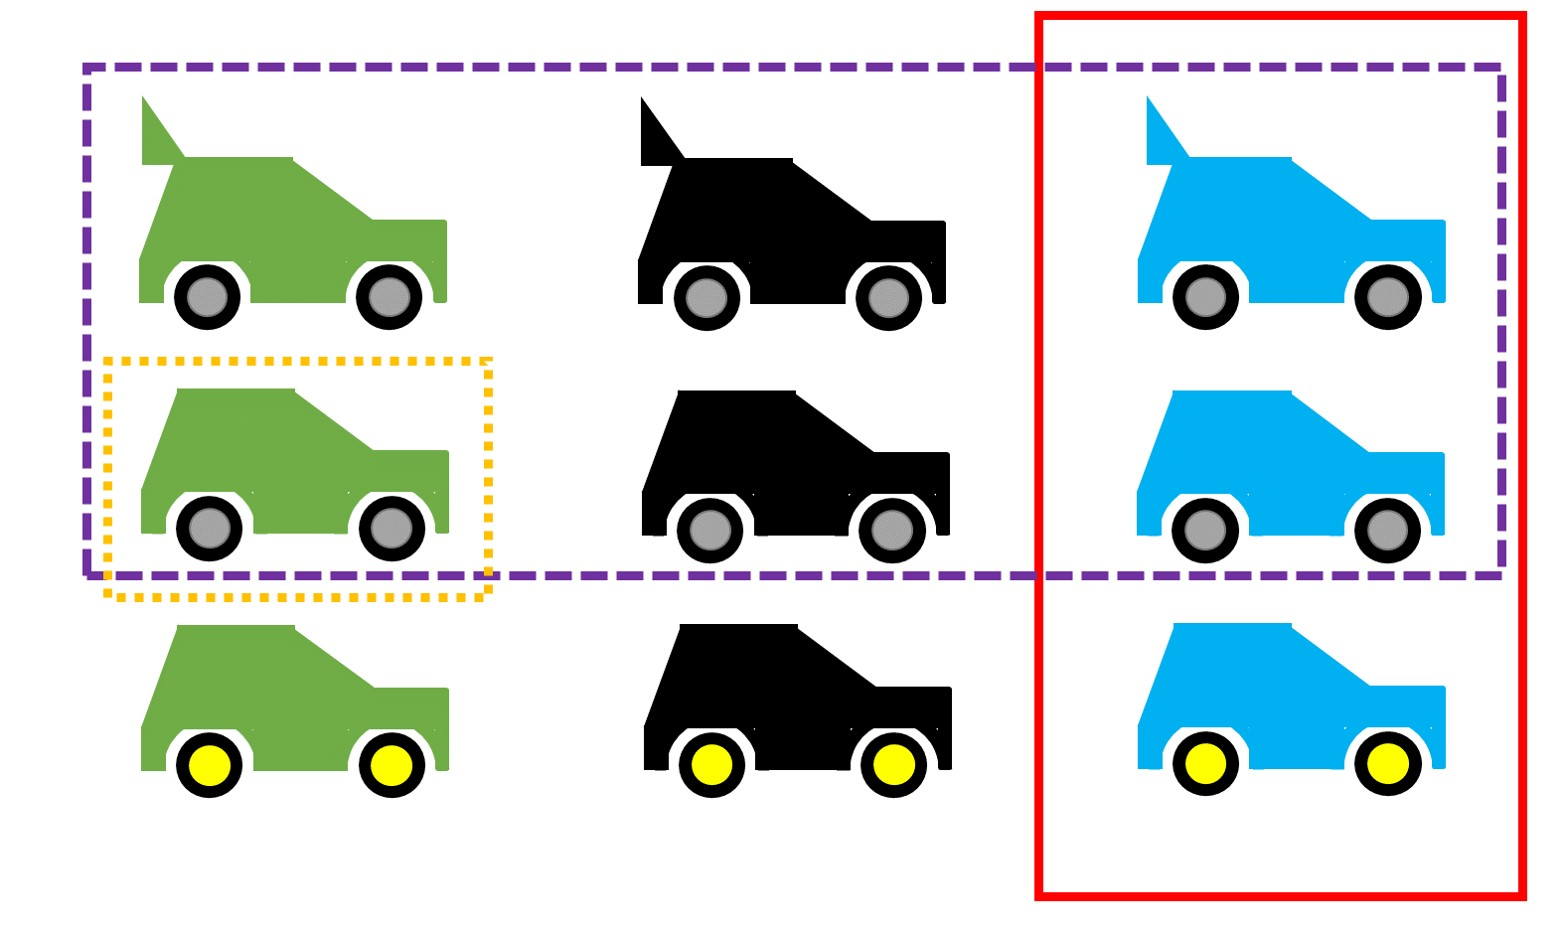
\includegraphics{images/empirischergehalt.jpg}

}

\caption{Visualisierung von Theorien mit unterschiedlichem empirischem
Gehalt}

\end{figure}%

\end{tcolorbox}

\subsection{Deduktion und Induktion}\label{deduktion-und-induktion}

Methoden werden reformiert und Wissenschaftler*innen diskutieren, wie
Wissenschaft funktioniert, ablaufen sollte, und welche Methoden sinnvoll
und unsinnig sind. Wie am hermeneutischen Zirkel klar wird, führt ein
Erkenntnisweg darüber, eine Menge von Beobachtungen zu einer
Regelmäßigkeit oder Gesetzmäßigkeit zusammenzufassen (\emph{Induktion})
und ein weiterer besteht daraus, aus einer Gesetzmäßigkeit bzw. Theorie
Vorhersagen über noch nicht angestellte Beobachtungen zu machen
(\emph{Deduktion}). Immer wieder wird diese Unterscheidung im
wissenschaftlichen Diskurs vernachlässigt oder ausgeblendet.
Beispielsweise drehte sich ein Dialog in der Konsumentenpsychologie
jahrelang darum, welcher Weg besser sei, obwohl beide Wege gleichermaßen
legitim sind und einander ergänzen (Calder, Phillips, and Tybout 1981).
Ähnlich verhält es sich bei Konflikten zwischen qualitativer und
quantitativer Vorgehensweise, die formal betrachtet jeweils eher
induktiv oder deduktiv vorgehen (Borgstede and Scholz 2021). Bei
Replikationsforschung hat traditionell die induktive Seite mehr
Beachtung erfahren (Hüffmeier, Mazei, and Schultze 2016; Yamashita and
Neiriz 2024): Jeder Unterschied zwischen Replikation- und Originalstudie
wird als mögliche Ursache für ein Scheitern des Replikationsversuches
herangezogen um die Vertrauenswürdigkeit der Originalbefunde
aufrechtzuerhalten (Baumeister and Vohs 2016). Dabei gerät außer Acht,
dass kleinere Unterschiede zwischen Original- und Replikationsstudie
(z.B. Verwendung der Maße, durchschnittliches Alter der
Versuchspersonen, Sprache der Instruktion) von Theorien nicht erfasst
werden -- ihnen zufolge also unerheblich sein sollten -- und eine
fehlgeschlagene Replikation klar die Grenzen der Theorie aufzeigt und
sich aus ihr Empfehlungen für die Modifikation von Theorien ableiten
lassen (Cesario 2014; Dijksterhuis 2014). Ein Überblick über die
Vorgehensweisen ist in der folgenden Tabelle.

\begin{longtable}[]{@{}
  >{\raggedright\arraybackslash}p{(\columnwidth - 4\tabcolsep) * \real{0.1318}}
  >{\raggedright\arraybackslash}p{(\columnwidth - 4\tabcolsep) * \real{0.3885}}
  >{\raggedright\arraybackslash}p{(\columnwidth - 4\tabcolsep) * \real{0.4797}}@{}}
\toprule\noalign{}
\endhead
\bottomrule\noalign{}
\endlastfoot
\textbf{Facette} & \textbf{Deduktives Vorgehen (Theorie-geleitet)} &
\textbf{Induktives Vorgehen (Phänomen-geleitet)} \\
Verallgemeinerbarkeit steckt in\ldots{} & der Theorie: Sie ist a priori
maximal allgemein (z.B. gilt sie, bis anderweitig nachgewiesen, für alle
Menschen). & den Daten: Erst vielfältige Beobachtungen in verschiedenen
Kontexten erlauben die Annahme, dass das Phänomen allgemeingültig
ist. \\
Veränderung von Verallgemeinerbarkeit & Mit mehr Beobachtungen sinkt die
Allgemeingültigkeit. & Mit mehr Beobachtungen steigt die
Allgemeingültigkeit (sofern sie bestätigender Natur sind). \\
Art der Prüfung & Vorhersagen der Theorie werden vorwiegend Versuchen
der \emph{Widerlegung} unterzogen. & Wiederholte Beobachtungen
\emph{bestätigen} den ursprünglichen Einzelfall. \\
Wahl des Studiensettings & Studentische Stichproben aus nur einem Land
oder Laboruntersuchungen sind unbedenklich. & Der Kontext der
Untersuchung sollte die Zielbedingungen (z.B. bei der Anwendung der
Erkenntnisse in der Praxis) möglichst gut widerspiegeln. \\
\end{longtable}

\emph{Merkmale induktiver und deduktiver Vorgehensweise, entnommen,
übersetzt, und angepasst aus einem unveröffentlichten Manuskript von
Röseler \& Leder.}

\subsection{Hilfshypothesen}\label{hilfshypothesen}

Über folgende Wege lassen sich Replikationsfehlschläge erklären:

\begin{enumerate}
\def\labelenumi{\arabic{enumi}.}
\item
  Fehler erster Art der Originalstudie: Der Originalbefund war nur ein
  Zufallsbefund oder kam durch wissenschaftliches Fehlverhalten zustande
  (siehe Kapitel „Freiheitsgrade von Forschenden (Researchers' Degrees
  of Freedom)``).
\item
  Fehler erster Art der Replikationsstudie: Die Originalstudie lag
  richtig, die Replikationsstudie hat einen Fehler gemacht (z.B. zu
  kleine Stichprobe, schlechte Kalibrierung der Instrumente, oder
  wissenschaftliches Fehlverhalten).
\item
  Grenzbereich des Phänomens: Beide Studien sind vertrauenswürdig. Die
  Replikationsstudie \emph{unterscheidet} sich auf eine für die Theorie
  wichtige Weise (z.B. wurde die Replikationsstudie mit Personen aus
  einem anderen Land durchgeführt und die Theorie gilt nur für Menschen
  aus dem „Original-Land'').
\end{enumerate}

Variante 3 ist konstruktiv und nimmt beide Einzelbefunde für robust hin.
Notwendig dafür ist ein theoretisch relevanter Unterschied zwischen der
Original- und Replikationsstudie, der durch die unendliche Anzahl
möglicher wichtiger Faktoren in den meisten Fällen zutrifft (Smedslund
2015). Über diesen Weg lässt sich die Theorie dann modifizieren oder
eine weitere Theorie aufstellen, die für den Kontext der Untersuchung
ebenfalls berücksichtigt werden muss. Schwierig wird es, wenn Forschende
nach bestem Wissen eine Replikation durchführen, diese ``fehlschlägt''
(also nicht das nachgewiesen wird, was nachgewiesen werden sollte), und
andere Forschende die Replikation dafür kritisieren, dass sie etwas
``falsch'' gemacht hat. Nachdem Hagger et al. (2016) unter Absprache mit
Roy Baumeister dessen Ego Depletion Theorie mit einer großangelegten
Studie prüften, kritisierten Baumeister and Vohs (2016), dass von Anfang
an zu erwarten gewesen wäre, dass die Studie nicht funktioniert und
bezeichnete die Studie als fehlgeleitet. Vohs, die Ko-Autorin der Kritik
war, führte einige Jahre später eine weitere groß angelegte
Replikationsstudie durch. Obwohl sie dieses Mal ihrem eigenen Rat folgen
konnten, konnten die Forschenden wieder nicht den erwarteten Effekt
finden (Vohs et al. 2021).

\section{Weiterführende
Informationen}\label{weiterfuxfchrende-informationen-1}

\begin{itemize}
\item
  Eine philosophie Perspektive auf den Zusammenhang zwischen Theorie,
  Messungen, und Replikationen diskutiert @ramminger2023vermessen
\item
  Yarkoni (2019) argumentiert, dass das Replikationsprobleme in der
  Verallgemeinerung von Ergebnissen zu Theorien ihren Ursprung haben.
\item
  Fanelli diskutiert in einem Vortrag die Komplexität von Forschung als
  Grund für Replikationsfehlschläge und schlägt eine Theorie zur Messung
  von Komplexität vor (Fanelli, Tan, et al. 2022), Ein Video zu einem
  Vortrag ist online verfügbar:
  \url{https://www.youtube.com/watch?v=CEAV7420jBk}
\end{itemize}

\subsection{Literatur}\label{literatur-11}

\chapter{Epistemische Probleme}\label{epistemische-probleme}

Epistemologie heißt Erkenntnislehre und ist ein Teilgebiet der
Philosophie. Darin wird diskutiert, wie Wissenschaft funktioniert, wie
Wissen produziert werden kann, oder worin der Unterschied zwischen
wissen und glauben liegt. Epistemologische Erklärungsansätze für
Replikationsfehlschläge übersteigen systemische und methodische
Faktoren, haben aber auch andere Prüfbarkeitsansprüche. Während
wissenschaftstheoretische Ansätze teilweise empirisch (also durch
Beobachtungen) prüfbare Vorhersagen erlauben, lässt sich über die
philosophischen Probleme nur nachdenken und diskutieren.

\subsection{Robustheit und Historizität von
Phänomenen}\label{robustheit-und-historizituxe4t-von-phuxe4nomenen}

Unter welchen Voraussetzungen ist es wenig überraschend, dass
Replikationsversuche fehlschlagen? Ein Ausweg ist anzunehmen, dass die
untersuchten Phänomene extrem empfindlich oder unstabil seien.
Regelmäßigkeiten im menschlichen Verhalten analog zu den
Planetenbewegungen zu entdecken könnte schlichtweg nicht möglich sein
(Smedslund 2015). Weniger extreme Annahmen über die Existenz von
Regelmäßigkeiten, die möglicherweise nicht jede Person ausnahmslos
betreffen aber „im Schnitt'' gelten. Lewin (1930) unterscheidet in
aristotelische und galileische Gesetzmäßigkeiten, wobei ersteres die
\emph{aristotelischen} sind, die in den Sozialwissenschaften relativ
unumstritten sind. Eine Regelmäßigkeit bzw. ein Naturgesetz im
aristotelischen Sinne kann zum Beispiel sein, dass Männer größer als
Frauen sind. Noch extremer ist die Theorie, dass Menschen sich des
Wissens über sie bewusst sind und ihr Verhalten dynamisch anpassen und
Verhaltenswissenschaften immer historisch bzw. zeitgebunden sind: Wird
herausgefunden, dass Menschen in ihren Entscheidungen tendenziell dazu
neigen nichts zu ändern, auch wenn sich dadurch ihre Situation
verbessern würde, wird ihnen diese Tatsache über die Wissenschaft vor
Augen geführt und sie können ihr Verhalten anpassen. Dabei handelt es
sich übrigens um den Status Quo Bias, bei dem Menschen die jetzige
Situation einer anderen vorziehen (Samuelson and Zeckhauser 1988; Xiao
et al. 2021).

Wie stark sich Phänomene durch vermeintlich kleinere Unterschiede im
Versuchsaufbau unterscheiden wurde bereits meta-wissenschaftlich
untersucht. Landy et al. (2020) ließen mehrere Hypothesen von mehreren
Forschenden prüfen und Faktoren, die laut den dahinterliegenden Theorien
eigentlich keinen Unterschied machen sollten, führten dazu, dass
Gegenteilige Ergebnisse entstanden. Auf Replikationsforschung übertragen
ist es also möglich, dass in bestimmten Forschungsbereichen völlig
unklar ist, unter welchen Bedingungen welche Zusammenhänge zu beobachten
sind.

\section{Weiterführende
Informationen}\label{weiterfuxfchrende-informationen-2}

\begin{itemize}
\item
  Fleck (1935/2015) schlägt eine Theorie des wissenschaftlichen
  Fortschritts vor, bei der Wissen immer einem sogenannten Denkstil
  unterliegt, der für die jeweilige gesellschaftliche Situation optimal
  ist. Dabei bedient er sich Elementen der Evolutionstheorie,
  Soziologie, und Psychologie.
\item
  Shiffrin, Börner, and Stigler (2018) diskutiert das scheinbare Paradox
  zwischen Fallibilität und Fortschritt in der Wissenschaft.
\end{itemize}

\subsection{Literatur}\label{literatur-12}

\part{Lösungen}

\part{Lösungen und Ansätze zur Verbesserung der Lage der Psychologie}

Werfen wir ein Blick darauf, was sich seit 2012 in der Psychologie
verändert hat. Eingeteilt sind die Veränderungen dahingehend, welchen
Teil des Problems sie vor allem betreffen: Ist der Zweck einer neuen
Vorgabe, das System, die Methodik, oder die Theorien der Forschung zu
verbessern? Einige Lösungen sind mit vielen Problemen gleichzeitig
verknüpft und manche sind auf bestimmte Angelegenheiten maßgeschneidert.
Die Abbildung enthält eine grobe Unterteilung.

\begin{figure}[H]

{\centering 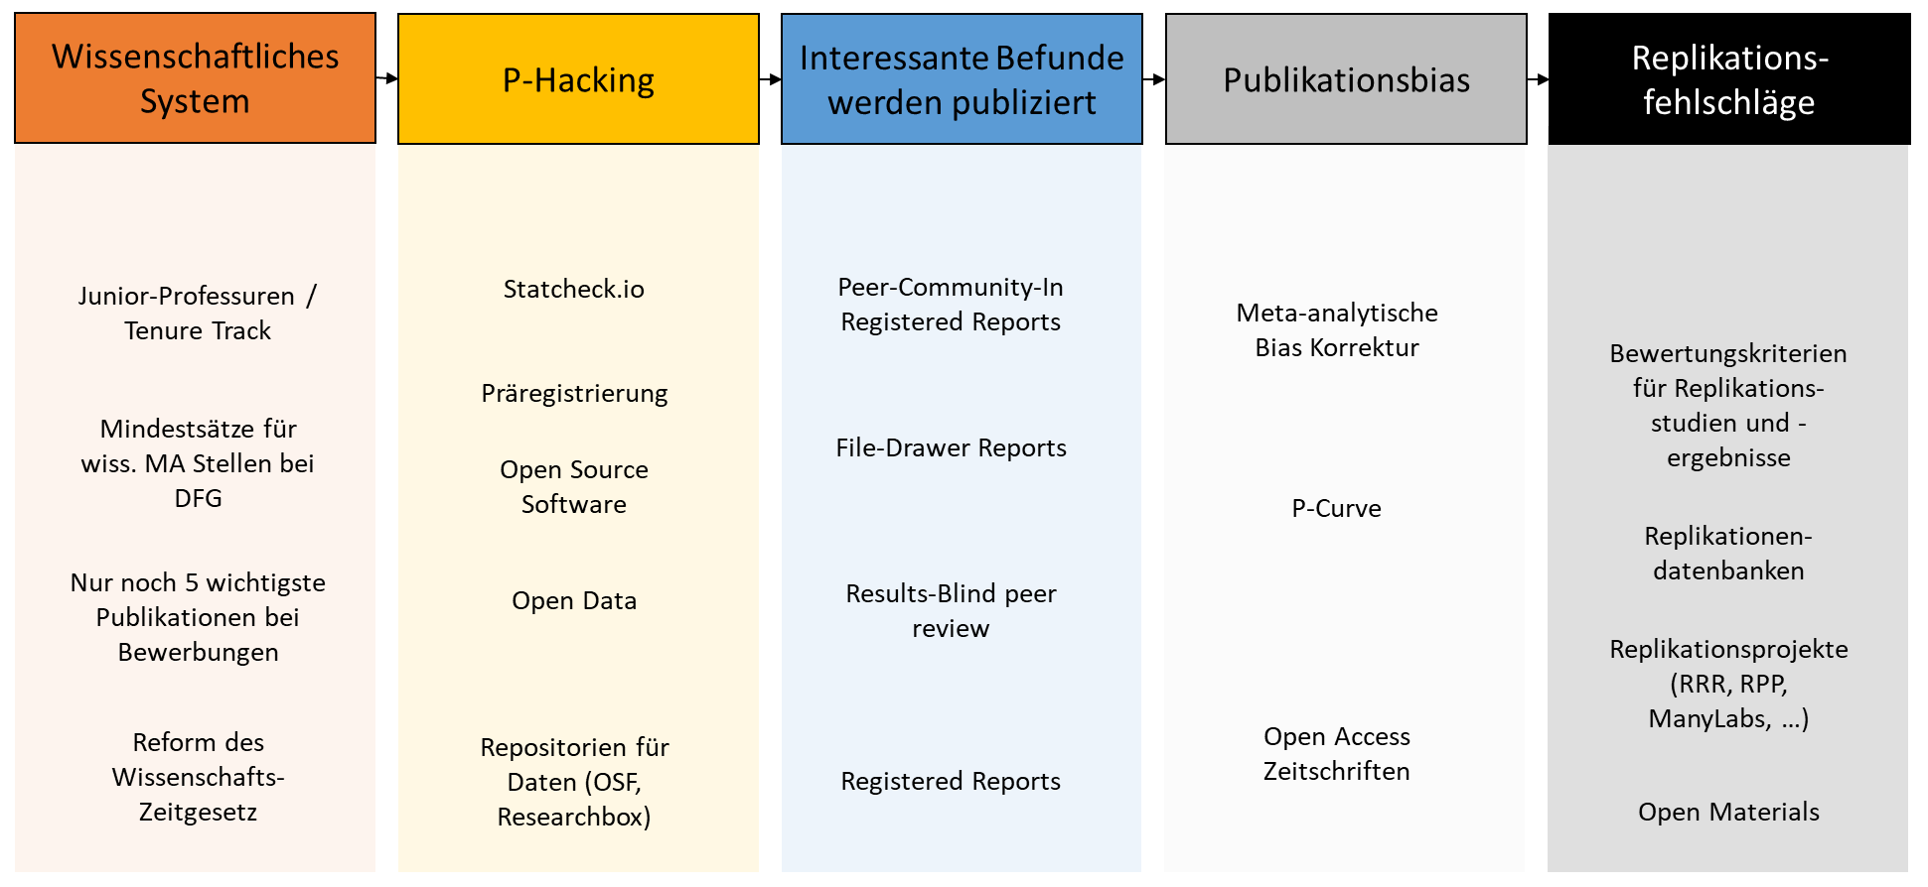
\includegraphics{images/lösungsansätze.png}

}

\caption{Lösungsansätze und welches Problem in der Wissenschaft sie
aufgreifen}

\end{figure}%

\section*{}\label{section}
\addcontentsline{toc}{section}{}

\markright{}

\chapter{Das System}\label{das-system-1}

Ansätze, die darauf abzielen, das System zu verändern, bergen am meisten
Potenzial, denn um im System Geld verdienen zu können, müssen Forschende
sich an die Regeln halten. Und solange Publikationen die Währung sind
und Paper mit knackigen Titeln und eindeutigen Ergebnissen als
qualitativ hochwertiger befunden werden, sind Forschende darin
motiviert, nach knackigen Titeln und eindeutigen Ergebnissen und nicht
nach der Wahrheit zu suchen.

Insgesamt ist eine positive Entwicklung sichtbar (Korbmacher et al.
2023) und eine Veränderung der Anreizstruktur wird anvisiert. Sie lässt
sich als Angleichung des wissenschaftlichen Systems an die
\emph{Mertonschen Normen} (nach Robert Merton) auffassen (Robert K.
Merton 1973): (1) Kommunismus: Das wissenschaftliche Wissen sollte allen
Wissenschaftler*innen gleichermaßen gehören, um die Zusammenarbeit zu
fördern. (2) Universalismus: Wissenschaftliche Güte ist unabhängig vom
soziopolitischen Status und persönlichen Attributen der Teilhabenden.
(3) Desinteresse: Wissenschaftliche Institutionen handeln im Interesse
der Wissenschaft und nicht für persönlichen Gewinn. (4) Organisierter
Skeptizismus: Wissenschaftliche Behauptungen sollten einer kritischen
Prüfung unterzogen werden bevor sie akzeptiert werden.

Nosek empfiehlt in einem
\href{https://www.cos.io/blog/strategy-for-culture-change}{Blogpost}
eine Maßnahmenstruktur, nach welcher die gewünschten Veränderung
nacheinander \ldots{}

\begin{enumerate}
\def\labelenumi{\arabic{enumi}.}
\tightlist
\item
  möglich (z.B. durch Infrastruktur wie online Repositorien, in denen
  Forschungsmaterialien öffentlich und gratis hochgeladen werden
  können),
\item
  einfach (z.B. durch barrierearme Angebote, mehrsprachige Anleitungen),
\item
  normativ (z.B. durch Wissenschaftliche Communities, die gemeinsam
  hinter Forderungen der Verbesserung stehen),
\item
  belohnend (z.B. durch designierte Preise), und
\item
  notwendig (z.B. durch Mindeststandards, die von Zeitschriften oder
  Drittmittelgebern gefordert werden)
\end{enumerate}

gemacht werden sollen. Wie die verschiedenen Ansätze bei den
verschiedenen Akteuren, also Politik, Universitäten, oder Zeitschriften
konkret aussehen, wird im Folgenden diskutiert.

\begin{figure}[H]

{\centering 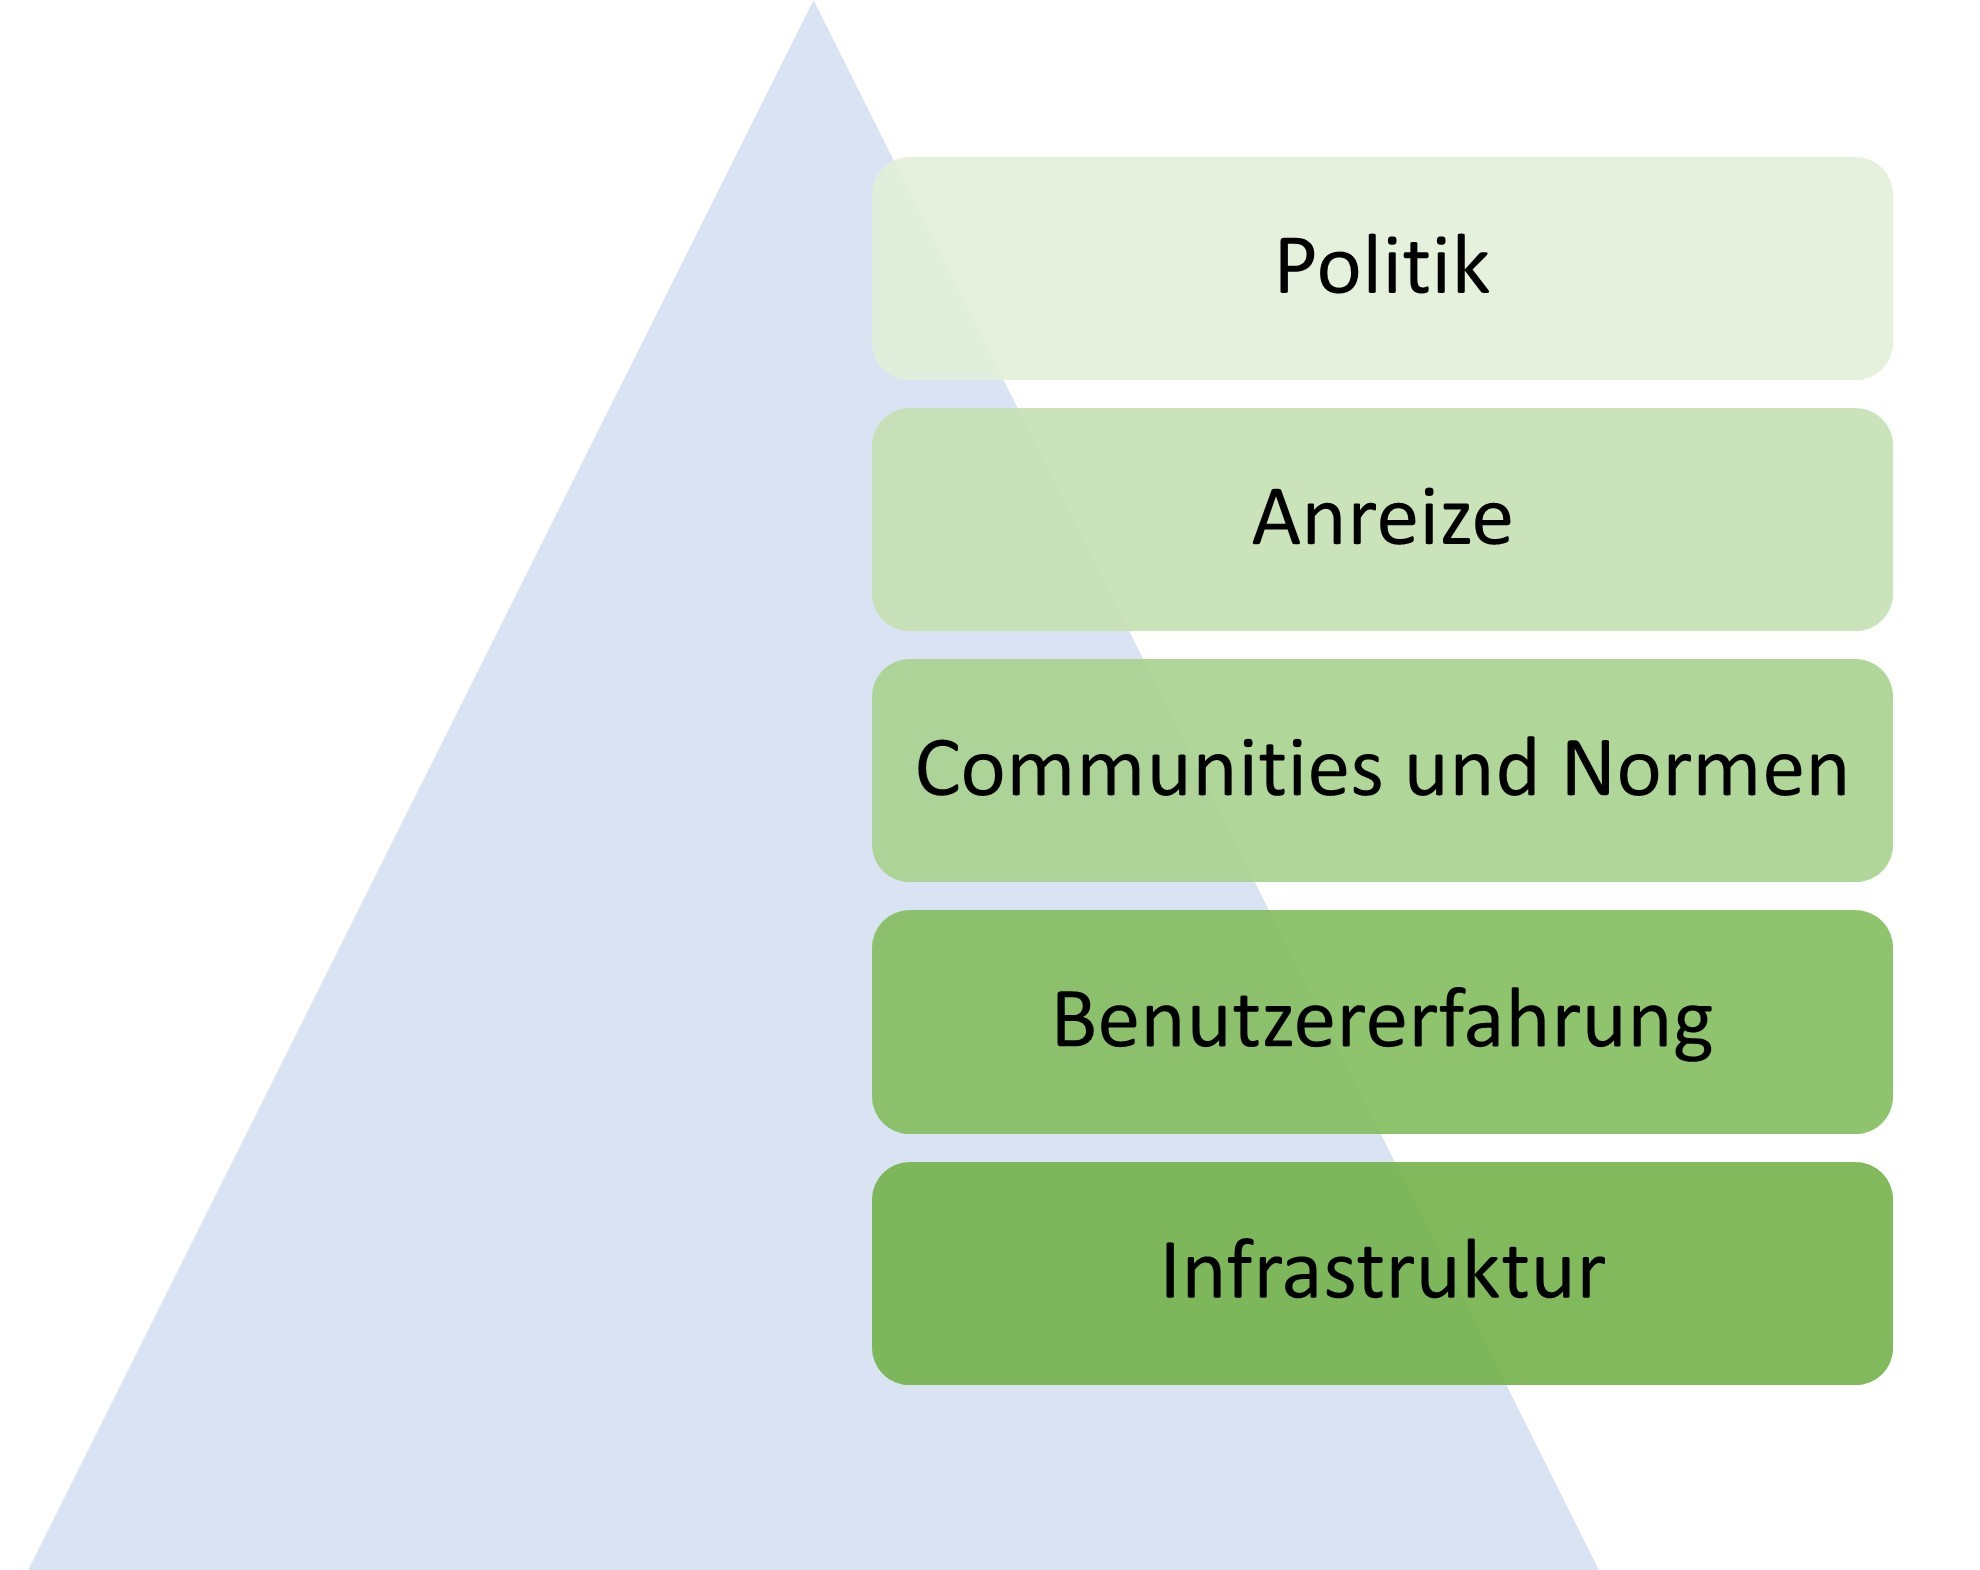
\includegraphics{images/pyramide.jpg}

}

\caption{Kulturwandel in der Wissenschaft nach Nosek
(https://www.cos.io/blog/strategy-for-culture-change)}

\end{figure}%

\subsection{Politik}\label{politik}

International stehen politische Parteien und Vereinigungen deutlich
hinter Open Science und Open Access. Beispielsweise empfiehlt die UNESCO
einen universellen Zugang zu wissenschaftlichen Wissen ungeachtet von
Herkunftsland, Geschlechterrolle, politischen Grenzen, ethnischer
Zugehörigkeit, oder ökonomischen oder technologischen Hürden {[}UNESCO
(2020); p.~3{]}.
\href{https://opusproject.eu/openscience-news/open-science-horizon-unescos-recommendation/}{Arbeitsgruppen}
für politische Instrumente, Förderung, und Infrastruktur wurden
entsprechend gegründet. Die
\href{G7\%20BEST\%20PRACTICES\%20FOR\%20SECURE\%20&\%20OPEN\%20RESEARCH\%20Security\%20and\%20Integrity\%20of\%20the\%20Global\%20Research\%20Ecosystem\%20(SIGRE)\%20Working\%20Group}{G7}
setzen sich für wissenschaftliche Integrität, akademische Freiheit, und
Open Science ein.
\href{https://www.consilium.europa.eu/en/press/press-releases/2023/05/23/council-calls-for-transparent-equitable-and-open-access-to-scholarly-publications/}{Offener
Zugang} aber auch
\href{Triggers\%20for\%20audits\%20of\%20good\%20laboratory\%20practice\%20(GLP)\%20studies}{Transparenz}
des wissenschaftlichen Vorgehens wird auch seitens der Europäischen
Union gefordert. Infrastruktur (z.B. die
\href{https://eosc-portal.eu}{European Open Science Cloud}) und diverse
Open Science Forschungsprojekte werden gezielt gefördert. Für alle durch
die EU geförderten Forschungsprojekte steht zudem die kostenlose
Publikations- und Begutachtungs-Plattform
\href{https://open-research-europe.ec.europa.eu}{Open Research Europe}
zur Verfügung.

In Deutschland hat sich die Regierung der Periode 2021-2025 im Rahmen
des Koalitionsvertrages vorgenommen, „Open Access \ldots{} als
gemeinsamen Standard {[}zu{]} etablieren.'' Einzelne Bundesländer wie
Nordrhein-Westfalen haben in Zusammenschlüssen aus den jeweiligen
Universitäten darüber hinaus Open \emph{Access} Strategien entwickelt
(Openness 2023a) und arbeiten aktuell an Open \emph{Science} Strategien.
Andere Länder, wie zum Beispiel Schweden, haben bereits
\href{https://www.kb.se/samverkan-och-utveckling/nytt-fran-kb/nyheter-samverkan-och-utveckling/2024-01-15-national-guidelines-for-promoting-open-science-in-sweden.html}{nationale
Richtlinien zu Open Science} entwickelt. Hinsichtlich der Problematik
von Machtmissbrauch wird das Problem beispielsweise in einem
Eckpunkte-Papier des Landes NRW anerkannt, doch als
\href{https://opal.landtag.nrw.de/portal/WWW/dokumentenarchiv/Dokument/MMV18-2422.pdf}{Einzelfall}-
statt System-Problem verstanden
(\href{https://www.jmwiarda.de/https-www.jmwiarda.de-2024-05-28-bitte-nachschaerfen/}{Kommentar
dazu}).

\subsection{Universitäten}\label{universituxe4ten}

\begin{tcolorbox}[enhanced jigsaw, title=\textcolor{quarto-callout-note-color}{\faInfo}\hspace{0.5em}{Welche Universitäten tun etwas? (Beispiele)}, colbacktitle=quarto-callout-note-color!10!white, rightrule=.15mm, titlerule=0mm, left=2mm, bottomrule=.15mm, arc=.35mm, leftrule=.75mm, toprule=.15mm, opacityback=0, breakable, bottomtitle=1mm, colframe=quarto-callout-note-color-frame, toptitle=1mm, opacitybacktitle=0.6, coltitle=black, colback=white]

Das Thema Open Science hat bei vielen Universitäten bereits Anklang
gefunden. Während die meisten deutschen Universitäten (zeitlich
begrenzte) Mittel für Open Access Publikationen haben, existieren an
einigen darüber hinaus Open Science Policys (z.B.
\href{https://oa-info.sh/2022/01/open-science-policy-der-uni-erlangen-nuernberg/}{FAU
Erlangen}), Open Science Centers (z.B.
\href{https://www.osc.uni-muenchen.de/index.html}{LMU Open Science
Center}; \href{https://oscc.uni-koeln.de/home}{Köln Open Science
Center}; \href{https://www.uni-muenster.de/MueCOS/}{Münster Center for
Open Science};
\href{https://www.uni-mannheim.de/open-science/open-science-office/}{Mannheim
Open Science Office}). Darüber hinaus unterstützen das
Leibniz-Informationszentrum Wirtschaft in Kiel und das Leibniz-Institut
für Psychologie Replikationsforschung beispielsweise mit einer
Replikationszeitschrift (\url{https://www.jcr-econ.org}) oder im Rahmen
einer Juniorprofessur für Psychologische Metawissenschaft. Eines der
größten Zentren für Metawissenschaft n Europas hat sich in den
Niederlanden in Tilburg gebildet. Die Berliner Universitäten haben eine
gemeinsame Open Access Erklärung entwickelt
(\url{https://openaccess.mpg.de/Berliner-Erklaerung}) und in Frankreich
ist die Universität Sorbonne ein Pionier: Gemeinsam mit der Universität
Amsterdam und dem Universitätscollege London wurde eine Erklärung über
die die Veröffentlichung von Forschungsdaten unterzeichnet. Seit 2024
hat die Universität Sorbonne darüber hinaus den Vertrag mit Clarivate
für die Nutzung der Forschungsdatenbank „Web of Science'' gekündigt und
arbeitet seitdem mit der Open Source Software „OpenAlex'' (Priem,
Piwowar, and Orr 2022).

\end{tcolorbox}

Für die langfristige Entwicklung der Wissenschaften haben Universitäten
dadurch eine besondere Verantwortung, dass sie Wissenschaftler*innen
beschäftigen und an ihnen die Auswahl für die wenigen unbefristeten
Arbeitsplätze in der Wissenschaft fallen. Wenn jahrzehntelang
Professuren auf Basis subjektiver, nicht-reproduzierbarer, und für gute
Wissenschaft nachrangigen Kriterien gewählt werden (z.B. Anzahl an
Publikationen in Fachzeitschriften), kann sich das negativ auf die
Entwicklung von Wissenschaften auswirken. Diesem Problem entgegenwirkend
wurde ein Forschungspreis des Berlin Institute of Health (BIH), der
jährlich für Projekte zur Förderung von wissenschaftlicher Integrität
verliehen wird, an ein Projekt, das objektive und sinnvolle
Auswahlkriterien für Professor*innen entwickelt vergeben (Schönbrodt,
Gärtner, Frank, Gollwitzer, Ihle, Mischkowski, Phan, Schmitt, Scheel,
Schubert, and others 2022; Gärtner, Leising, and Schönbrodt 2022a). Um
die Rolle quantiativer Indikatoren zu schwächen wird bereits an einigen
Universitäten und bei DFG-Anträgen die ``N-best'' bzw. häufig ``5-best''
Regel angewandt (Frank 2019): Dabei dürfen nur die 5 besten
Forschungsartikel in der Bewerbung genannt werden und die Evaluation
darf nur auf Basis von ihnen geschehen.

Innerhalb von Universitäten spielen außerdem die Bibliotheken eine
aufklärerische Rolle hinsichtlich Forschungsdatenmanagement und
Publikationskultur (Schmidt et al. 2024). Über sie kann der
Forschungsprozess mit entsprechender Infrastruktur (z.B. zum Lagern und
Veröffentlichen von Forschungsmaterialien und -ergebnissen) unterstützt
werden (Quan 2021) und verhindert werden, dass sich eine „Abhängigkeit
von wenigen kommerziellen Anbietern'' ergibt, die „begrenzen, was
{[}bei{]} der Forschung an Arbeitsmöglichkeiten und Fragestellungen
erreichbar ist'' (Siems 2024). Eine Pflicht, Mitglieder eine Universität
zur Einhaltung von Open Science Strategien zu bewegen, gibt es an
Universitäten durch den hohen Stellenwert der „Freiheit der Forschung''
kaum. Damit könnten sie Gefahr laufen, für Forschende weniger attraktiv
zu werden: Wenn beispielsweise auf namhafte Zeitschriften nicht mehr
über die Universität zugegriffen werden kann, weil Verträge mit
closed-access Zeitschriften gekündigt wurden, erschwert das den
Forschenden die Arbeit. Beispielsweise klagte die juristische Fakultät
der Universität Konstanz gegen eine
Zweitveröffentlichungs\emph{pflicht}: Forschende in Deutschland haben
das \href{https://de.wikipedia.org/wiki/Zweitveröffentlichung}{Recht zur
Zweitveröffentlichung}, das heißt, dass sie ihre Forschung, wenn sie in
einer Fachzeitschrift veröffentlicht wurde, auch selbst (z.B. über
eigene Websites) veröffentlichen dürfen. In Konstanz konnten die
Forschenden nicht dazu verpflichtet werden, davon Gebrauch zu machen.

Ein weiteres Stellrad von Universitäten ist die Bezuschussung von
Publikationskosten bei Zeitschriften. Wird beispielsweise die
wissenschaftliche Qualität einer Zeitschrift angezweifelt, kann eine
Universität diese
\href{https://www.suub.uni-bremen.de/ueber-uns/neues-aus-der-suub/unter-kritischer-beobachtung-open-access-publikationen-im-mdpi-verlag}{Bezuschussung
stoppen}.

Eine oft vernachlässigte Rolle kommt außerdem der universitären Lehre
hinzu. Durch die Freiheit von Forschung und Lehre und bereits
durchgeplanten Studiengängen gestaltet sich die Integration neuer Themen
wie Open Science schwierig. Forschende, in deren Lehre die Thematik eine
Rolle spielt, teilen proaktiv ihre Materialien, erstellen gemeinsam
Curricula, und sind beispielsweise in großen internationalen Initiativen
wie dem Framework for Open and Reproducible Research Training
(\href{https://forrt.org}{FORRT.org}) vernetzt (konkrete Vorschläge zur
Integration von Open Science in die Lehre hat zum Beispiel C. R.
Pennington and Pownall (2024) veröffentlicht.

\subsection{Institute und
Vereinigungen}\label{institute-und-vereinigungen}

Wissenschaftliche Gebiete leben vor allem durch Communities, also alle
in dem Bereich forschenden Personen. Sie organisieren sich in Vereinen
(z.B. Deutsche Gesellschaft für Psychologie), Interessensverbunden, oder
ähnlichen Gemeinschaften. Eine besondere Stellung hat in Deutschland die
Deutsche Forschungsgemeinschaft, welche staatlich und über die
Bundesländer mit mehreren Milliarden Euro ausgestattet Forschungsgelder
vergibt. Als eine der wichtigsten nationalen Institution hat ihre Open
Science Positionierung einen hohen Stellenwert (Deutsche
Forschungsgemeinschaft 2022). Erfahrungsgemäß gehen Veränderungen jedoch
nicht von der DFG aus, sondern die DFG wartet auf Anstöße aus den
Fächern. In der Psychologie fördert darüber hinaus das
\href{https://leibniz-psychology.org/das-institut}{ZPID} die
Infrastruktur durch Zeitschriften, Pre-Print Server, und weitere
Methoden und in den Wirtschaftswissenschaften verwaltet das ZBW wichtige
Informationen oder Zeitschriften (REF). Auch interdisziplinäre
Vereinigungen wie das \href{https://openscience.cern}{CERN} oder
internationale Akteure wie die
\href{https://www.apa.org/pubs/journals/resources/publishing-tips/transparency-openness-promotion-guidelines?utm_campaign=apa_publishing&utm_medium=direct_email&utm_source=businessdevelopment&utm_content=openscience_promo_11302023&utm_term=text_middle_learnmore}{American
Psychological Association} verpflichten sich zu Offenheit und
Transparenz.

Im Rahmen der Open Science Reform entstanden außerdem viele neue
Vereinigungen. Das interdisziplinäre und besonders von
Wissenschaftler*innen in der frühen Karrierephase geleitete FORRT
(Azevedo et al. 2019) setzt sich für eine Verankerung von Open Science
in der Lehre ein. Der Verbesserung psychologischer Forschung hat sich
die Society for the Improvement of Psychological Science (SIPS)
verschrieben. Sogenannte „grassroot''-Initiativen (also von jungen
Wissenschaftler*innen ausgehende Bewegungen) haben sich an zahlreichen
Universitäten herausgebildet und zu Netzwerken wie dem
\href{https://osf.io/tbkzh/}{Netzwerk der Open Science Initiativen
(NOSI)} und „Reproducibility Networks'' wie dem deutschen Netzwerk
\emph{GRN} (\url{https://reproducibilitynetwork.de}), dem im Vereinigten
Königreich \emph{UKRN} (\url{https://www.ukrn.org}) und weiteren
zusammengeschlossen. Aber auch Zusammenschlüsse von Professor*innen zur
Änderung von Kurzzeitverträgen existieren (z.B. Netzwerk Nachhaltige
Wissenschaft, \url{https://netzwerk-nachhaltige-wissenschaft.de}).

\subsection{Zeitschriften}\label{zeitschriften}

Wissenschaftliche Zeitschriften gelten als Bühne des wissenschaftlichen
Diskurses und bestimmen maßgeblich, welche Elemente des
Forschungsprozesses zum „scientific record'' gehören und damit relevant
sind. Sie sind darüber hinaus als Organisatorinnen des
Begutachtungsprozesses für die Qualitätssicherung in der Wissenschaft
verantwortlich. Dem Mangel an Qualität entgegnend existieren bereits
ausführliche Empfehlungen zur Gestaltung von Zeitschriften, es bilden
sich neue Zeitschriften, und vollständige neue Begutachtungs- und
Publikationsmodelle werden vorgeschlagen und vielseitig implementiert.
Das Journal of \href{https://joss.theoj.org}{Open Source Software}
basiert beispielsweise auf einem öffentlich einsehbaren Programmiercode
und seine Infrastruktur lässt sich für weitere Zeitschriften einfach
kopieren und anpassen.

\subsubsection{Empfehlungen}\label{empfehlungen}

Herausgeber*innen, die sich in Bezug auf die von ihnen verwaltete
Zeitschrift mit Open Science Praktiken auseinandersetzen möchten, können
inzwischen auf einen umfangreichen Leitfaden zurückgreifen (Silverstein
et al. 2023). Über eine Diskussionsplattform (Journal Editors Discussion
Interface, JEDI) wurden Vorschläge gesammelt und es wird erklärt, worum
es sich bei Dingen wie Registered Reports, Open Peer Review,
Diversifizierung, und Open Access handelt und wie diese in eine
Zeitschrift implementiert werden können. Eventuelle Sorgen und Ängste
werden angesprochen und beantwortet. Das Committee on Publication Ethics
(COPE) setzt sich ebenfalls für Aufklärung und Lehre ein, die
Herausgeber, Universitäten, und Forschungsinstitute im Umgang mit
Problemen im Publikationssystem helfen soll. Es bietet beispielsweise
\href{https://publicationethics.org/retraction-guidelines}{Richtlinien}
unter welchen Umständen Publikationen zurückgezogen oder korrigiert
werden sollten, oder welche ethischen Standards ein
\href{https://publicationethics.org/resources/guidelines/cope-ethical-guidelines-peer-reviewers}{Begutachtungsprozess}
erfüllen sollte. Herausgeber*innen, die Zeitschriften für kommerzielle
Verlage verwalten und auf Systeme umsteigen möchten, die vollständig in
der Hand der Forschenden liegen, können über Universitätsbibliotheken
Hilfe bei der Migration von den kommerziellen zu offenen und
kostenfreien Systemen erhalten und Zeitschriften beispielsweise mit dem
Open Journal System verwalten (siehe z.B.
\href{https://ojs-de.net/start}{OJS Netzwerk}). Eine Datenbank mit
bereits über 20,000 offen zugänglichen Zeitschriften verwaltet das
Directory of Open Access Journals (\href{https://doaj.org}{DOAJ}).
Gutachter*innen von Forschungsartikeln können über die Reviewer Zero
Initiative (\url{https://www.reviewerzero.net}) auf Lehrmaterialien und
Leitfäden zugreifen (\url{https://osf.io/e7z5k/wiki/Resources/}).

\subsubsection{Open Science Praktiken
hervorheben}\label{open-science-praktiken-hervorheben}

Aus der Psychologie ist lange bekannt, dass Motivation über Belohnung
besser funktioniert als über Bestrafung (REF). Im Straßenverkehr, in dem
es bis vor einiger Zeit nur Bestrafungen für Verletzen von Regeln gab,
äußert sich die Erkenntnis beispielsweise an Geschwindigkeitstafeln, die
den Autofahrer*innen beim Einhalten des Tempolimits einen fröhlichen
Smiley zurückmelden. Wissenschaftliche Zeitschriften heben Einhaltung
von Empfehlungen (z.B. öffentlich verfügbare Datensätze) mit Plaketten
(\emph{Badges}) hervor. Die Zeitschrift \emph{Psychological Science}
geht dabei seit 2024 so weit, dass Badges schon wieder abgeschafft
werden und Open Science dort der Standard für alle Artikel ist. Auf der
Website topfactor.org sind Zeitschriften und deren Einhaltung
verschiedener Standards aufgelistet und in einer Rangliste abgebildet.
Zuletzt besteht in jedem System mit Belohnungen das Problem, dass die
Akteure ihr Verhalten auf die Belohnungen hin ausrichten und dabei
versuchen, Abkürzungen zu gehen (Klonsky 2024).

\subsubsection{Review Systeme}\label{review-systeme}

Wissenschaft zeichnet sich durch Systematik aus (Hoyningen-Huene 2013).
Der wohl systematischste Weg, die wissenschaftliche Qualitätssicherung
zu garantieren, wäre eine Studie, die verschiedene Systeme vergleicht.
Während aktuelle Forschung ähnliches unternimmt (Soderberg et al. 2021),
werden alternative Begutachtungssysteme aktuell ausprobiert. Zur
Erinnerung: Wissenschaftler*innen verfassen Artikel, die sie bei
Zeitschriften einreichen. Dort ist eine Person (Editor) dafür zuständig,
dass der Artikel, sofern er zur Zeitschrift passt, an Gutachtende
gesendet wird.

Um zu prüfen, ob die Urteile im Begutachtungsprozess zwischen den
Urteilenden übereinstimmen, haben Etzel et al. (2024) verschiedene
Gutachtende hinsichtlich klassischer Kriterien befragt. Sie fanden
heraus, dass das nicht der Fall ist und schlagen Kriterien vor, die
einen klaren Wert haben, und sich gut erfassen lassen (z.B. ob Daten
öffentlich verfügbar sind).

\paragraph{Open Peer Review}\label{open-peer-review}

Seit der Auseinandersetzung Forschender mit dem Begutachtungssystem wird
darüber hinaus diskutiert, was mit Gutachten passiert: Traditionell
bleiben sie unter Verschluss. In der Fachzeitschrift erscheint der
finale Artikel und alle vorherigen Versionen sind nur Autor\emph{innen,}
Herausgeber\emph{in,} und Gutachter*innen bekannt. Diese bleiben zudem
meistens anonym, das heißt, wenn sie sich keine Mühe gegeben haben, wird
es wahrscheinlich nie auffallen. Außerdem haben Forschende keinen
Anreiz, Gutachten zu verfassen - höchstens erhalten sie einen Nachweis,
dass sie ein Manuskript bei einer Zeitschrift begutachtet haben. Einige
Zeitschriften haben inzwischen das \emph{Open Peer Review} eingeführt.
Der Name passt nur halb, denn veröffentlicht werden Gutachten nur dann,
wenn der Artikel bei der Zeitschrift akzeptiert wird. Das birgt die
Gefahr, dass schwerwiegende Probleme, welche für eine Ablehnung
üblicherweise nötig sind, nicht ans Licht kommen. Forschende können den
Artikel dann ohne Überarbeitung bei einer anderen Zeitschrift
einreichen, wo die Probleme vielleicht nicht entdeckt werden. Dieses
Vorgehen führt zu Doppelarbeit und enormen Kosten (Aczel, Szaszi, and
Holcombe 2021). Zoltan Kekecs merkte dazu bei einer Diskussion im Rahmen
einer Konferenz an, dass selbst Kasinos, die in Konkurrenz zueinander
stehen, Listen von Betrüger\emph{innen miteinander austauschen.
Herausgeber}innen von Zeitschriften tun das noch nicht.

\begin{longtable}[]{@{}
  >{\raggedright\arraybackslash}p{(\columnwidth - 4\tabcolsep) * \real{0.2298}}
  >{\raggedright\arraybackslash}p{(\columnwidth - 4\tabcolsep) * \real{0.5021}}
  >{\raggedright\arraybackslash}p{(\columnwidth - 4\tabcolsep) * \real{0.2681}}@{}}
\toprule\noalign{}
\begin{minipage}[b]{\linewidth}\raggedright
Gutachten bleiben unter Verschluss
\end{minipage} & \begin{minipage}[b]{\linewidth}\raggedright
Gutachten werden bei Publikation veröffentlicht
\end{minipage} & \begin{minipage}[b]{\linewidth}\raggedright
Gutachten werden bei Publikation und Ablehnung veröffentlicht
\end{minipage} \\
\midrule\noalign{}
\endhead
\bottomrule\noalign{}
\endlastfoot
Es ist kein Nachweis der Qualitätskontrolle möglich. & Abgelehnte
Artikel können bei anderen Zeitschriften ohne Überarbeitung eingereicht
werden und führen zu Mehraufwand. & Qualitätskontrolle ist
nachvollziehbar und transparent. \\
\end{longtable}

Umstrittener als die Veröffentlichung von Gutachten ist die Anonymität
der Gutachter\emph{innen: Der Standard ist, dass Gutachten anonym sind,
aber bei Wunsch unterzeichnet werden können. Promovierende, die einen
Artikel eines potenziellen zukünftigen Chefs oder einer zukünftigen
Chefin schlecht beurteilen, werden dadurch geschützt. Selbst
Professor}innen können bei negativen Beurteilungen riskieren, dass der
oder die Kollegin später einen Forschungsgelderantrag von ihnen
begutachtet und sich für die Kritik rächt. Auf der anderen Seite kann
Anonymität zur Folge haben, dass Kritik gegen die Person gerichtet ist
und nicht konstruktiv ist.

Eine weitere Art, wie Peer-Review offen sein kann, ist, dass sich jede
Person daran beteiligen kann. Das ist zum Beispiel bei Meta-Psychology
möglich. Problematisch ist dabei jedoch die relativ geringe Beteiligung.
Bei den Zeitschriften Zeitschrift Synlett und ASAPbio werden Gruppe dazu
koordiniert, wie es sie zur Diskussion spannender Artikel schon in Form
von \emph{Journal Clubs} gibt - nur eben als
``\href{https://asapbio.org/crowd-preprint-review}{Pre-Print Review
Club}''.

\paragraph{Begutachtung von
Pre-Prints}\label{begutachtung-von-pre-prints}

\begin{tcolorbox}[enhanced jigsaw, title=\textcolor{quarto-callout-tip-color}{\faLightbulb}\hspace{0.5em}{Was ist ein Pre-Print?}, colbacktitle=quarto-callout-tip-color!10!white, rightrule=.15mm, titlerule=0mm, left=2mm, bottomrule=.15mm, arc=.35mm, leftrule=.75mm, toprule=.15mm, opacityback=0, breakable, bottomtitle=1mm, colframe=quarto-callout-tip-color-frame, toptitle=1mm, opacitybacktitle=0.6, coltitle=black, colback=white]

Ein Pre-Print nennt man ein Manuskript \emph{in dem} oder \emph{vor dem}
Stadium der Einreichung bei einer Zeitschrift. Es wurde möglicherweise
noch nicht begutachtet oder nach Begutachtung abgelehnt, auf einer
Internetseite veröffentlicht, ist zitierbar, und kostenlos zugängig. In
manchen Fällen mag es sinnvoll sein, ein wissenschaftlichen Beitrag
\emph{nicht} der Begutachtung zu unterziehen (z.B. bei Kommentaren,
Positions-Artikel, oder öffentlichem Austausch). Typischerweise zählen
begutachtete Beiträge für die wissenschaftliche Karriere mehr. Der Zweck
von Pre-Prints ist vielfältig: Sie erhöhen die Verfügbarkeit von Wissen,
erlauben eine schnellere Veröffentlichung (Beweise in der Mathematik
müssen aufwändig im Laufe von bis zu mehreren Jahren nachgeprüft
werden), und verhindern, dass einem andere Forschende mit einer
innovativen Idee zuvorkommen. In der Medizin und den
Sozialwissenschaften wurden sie aufgrund des schnelleren Austausches im
Zuge der Corona-Pandemie ausgiebig verwendet (Fraser et al. 2020). In
der Epidemilogie konnte nicht nachgewiesen werden, dass Pre-Prints
qualitativ schlechter sind (L. Nelson et al. 2022).

\end{tcolorbox}

Über Plattformen und Gemeinschaften wie \emph{PCI} oder
\emph{f1000research} werden Pre-Prints begutachtet. Sie werden dann
nicht bei einer Zeitschrift sondern bei dem der jeweiligen Einrichtung
eingereicht und dort begutachtet. Die Qualitätssicherung wird also von
Forschenden selbst organisiert und ist unabhängig von kommerziellen
Verlagen. Das Modell bei PCI ist, dass Artikel, die dort ein positives
Gutachten erhalten haben, ohne weiteres Gutachten bei einer der
teilnehmenden (\emph{PCI-friendly}) Zeitschriften veröffentlicht werden
können. Auf F1000research.com fungiert wie eine Zeitschrift, bei der
Artikel direkt zugängig sind, sich über die Zeit durch Peer Review
verändern. Auf ähnliche Weise gibt es bei der Zeitschrift für digitale
Geisteswissenschaften eine Peer-Review-Ampel: Nach Einreichung sind
Artikel dort direkt verfügbar und eine Ampel gibt an, ob sie unter
Begutachtung sind, und falls sie begutachtet wurden, ob es (noch)
schwerwiegende Probleme gibt oder nicht.

\paragraph{Gedächtnis von Gutachten}\label{geduxe4chtnis-von-gutachten}

Eine weitere Möglichkeit, Gutachten fest an Forschungsartikel
``dranzuheften'', besteht über Plattformen, die eine schnelle
Kommentierung ermöglichen. Zum Beispiel lassen sich über Pubpeer.com
oder hypothes.is alle wissenschaftlichen Beiträge (z.B. auch Daten)
öffentlich und wenn gewünscht anonym kommentieren. Das ist für
Pre-Prints möglich, sodass diese Kommentare dann dauerhaft damit
verknüpft sind. Mittels Plug-Ins für Internetbrowser werden dann
Artikel, zu denen es bei Pubpeer Diskussionen gibt, markiert. Weitere
Plattformen sind alphaxiv.org, Disqus, oder scirev.org.

\subsubsection{Aufmerksamkeit zum Thema in bestehenden
Zeitschriften}\label{aufmerksamkeit-zum-thema-in-bestehenden-zeitschriften}

Anforderungen an wissenschaftliche Artikel seitens der Zeitschriften
sind 2010 maßgeblichen Änderungen untergangen. In den
Sozialwissenschaften orientieren sich zahlreiche Zeitschriften an den
Richtlinien zur „Transparency and Openness Promotion'' (TOP) und
erhalten entsprechende TOP-Faktoren
(\url{https://topfactor.org/summary}). Dabei wird festgehalten, welcher
Grad an Offenheit und Transparenz von Forschungsdaten und -materialien
gefordert wird und ob Replikationen bei der jeweiligen Zeitschrift
veröffentlicht werden. Neue Herausgeber*innen bei existierenden
Zeitschriften haben große Änderungen vorgenommen. Beispielsweise haben
Hardwicke and Vazire (2023) für die Zeitschrift \emph{Psychological
Science} ein standardmäßiges Nachrechnen aller berichteten Ergebnisse ab
2024 angekündigt, indem sie mit dem Institute for Replication
zusammenarbeiten (\url{https://i4replication.org}). Vereinzelt haben
Zeitschriften Spezialausgaben herausgegeben, bei denen der Fokus auf
Replikationsstudien oder der Reproduzierbarkeit von Ergebnissen lag
(Carriquiry, Daniels, and Reid 2023).

\subsubsection{Zeitschriften für ``nicht
Innovatives''}\label{zeitschriften-fuxfcr-nicht-innovatives}

Durch die Selektion spannender Ergebnisse gibt es für Forschung, die
nicht bahnbrechend und dennoch höchst relevant ist, keine Plattform.
Schätzungen zufolge werden bis zu 40\% aller durchgeführten Studien
innerhalb von 4 Jahren nach Durchführung nicht veröffentlicht (Ensinck
and Lakens 2023). Andere Forschende können nicht davon lernen und
Ressourcen, die in die Sammlung und Auswertung der Daten geflossen sind,
Zeit von Versuchspersonen, und lange Vorbereitungen der Forschung werden
schließlich verschwendet. Zur Lösung dieses Problems haben sich neue
Zeitschriften und Formate gebildet. In der Ökonomie hat sich auf
Forderungen (Zimmermann 2015) hin beispielsweise eine
\href{jcr-econ.org}{Zeitschrift} für Replikationen und Kommentare
gebildet. Die Zeitschrift Meta-Psychology bietet ein Format für
Replikationen und eines für „Schubladenberichte'' an. Letzteres ist für
Studien vorgesehen, die wegen wenig überraschenden Ergebnissen oder
Fehlern in der Durchführung anderweitig in der Schublade landen würden
aber dennoch wichtige Informationen beinhalten. Ebenfalls zur Abbildung
des für den Forschungsprozess typischen Fehlschlagens wurde das
\href{https://journal.trialanderror.org}{Journal of Trial and Error}
gegründet, und bei \href{https://rescience.github.io/board/}{ReScience
C} und \href{rescience.org/x}{Rescience X} können Berichte über
Reproduzierbarkeit und Replikationen veröffentlicht werden.

\subsubsection{Publikationsmodelle}\label{publikationsmodelle}

Noch radikalere Vorschläge als die Anpassung bisheriger Zeitschriften
ist der Vorschlag, das bisherige System durch ein neues zu ersetzen.
Dabei handelt es sich um ein soziales Dilemma, bei dem Millionen von
Forschenden sich plötzlich anders verhalten müssen und dabei entgegen
der Spielregeln des wissenschaftlichen Systems handeln müssen (Brembs et
al. 2023). Das Dilemma wurde von kommerziellen Verlagen gestaltet,
welche daraus Geld verdienen. Brembs et al. (2023) haben einen präzisen
Vorschlag erarbeitet, bei welchem ein dezentrales System aufgebaut wird,
das soziale Netzwerke wie Mastodon als Vorbild hat, von
Wissenschaftler*innen organisiert wird, und Forschungsprodukte wie Daten
oder Programme ebenso wie die traditionellen Forschungsberichte
wertschätzt. Plattformen, die ein solches Mikro-Publishing-System
bereits implementieren sind
\href{https://www.researchequals.com/}{Research-Equals} oder Octopus.ac
(\textbf{Hsing?}). Dem System, bei dem alle Produkte begutachtet werden,
der Begutachtungsprozess aber nicht die Qualität sicherstellt, stehen
hier Ampel-Systeme und öffentliche Kommentierung entgegen, die
signalisieren, was und ob begutachtet wurde, welche Kritikpunkte
vorlagen, und wie damit umgegangen wurde.

\subsection{Forschende}\label{forschende}

Unabhängig von Nationalität, Wissenschaftsgebiet, und Universität haben
viele Forschende ihre Arbeitsweisen im Zuge von Open Science überdacht
und angepasst. \href{http://www.researchtransparency.org}{Hunderte}
haben öffentliche Erklärungen zur Forschungstransparenz und der
Forderung von Open Science Praktiken in der Rolle von
\href{https://www.opennessinitiative.org}{Gutachter*innen}
unterzeichnet. Einzelne Forschende führen im Rahmen von Lehre
Replikationsstudien durch (Boyce, Mathur, and Frank 2023; Jekel et al.
2020; Korell, Reinecke, and Lott 2023a), schließen sich weltweit
zusammen um gemeinsam Projekte durchzuführen, die einzelne nicht stemmen
könnten (z.B. Psychological Science Accelerator,
\url{https://psysciacc.org}), und entwickeln
\href{https://docs.google.com/spreadsheets/d/1KUMSeq_Pzp4KveZ7pb5rddcssk1XBTiLHniD0d3nDqo/edit\#gid=0}{Informations-Sammlungen}
(Open Scholarship Knowledge Base, https://oercommons.org/hubs/OSKB),
\href{https://osf.io/jfh3t/}{Leitfäden} und Glossare (Parsons et al.
2022), um den Zugang zu Open Science zu erleichtern. Eine noch
unerfüllte Forderung ist die, Forschende das System über
Zusammenschlüsse im Rahmen von Gewerkschaften zu reformieren (Rahal,
Fiedler, Adetula, Berntsson, Dirnagl, Feld, Fiebach, Himi, Horner,
Lonsdorf, and others 2023).

\subsection{Bewertungskriterien}\label{bewertungskriterien}

Mit der San Francisco Erklärung zur Forschungsbewertung (Declaration on
Research Assessment,
\href{https://sfdora.org/read/read-the-declaration-deutsch/}{SF DORA})
begannen 2012 viele Institutionen und Forschende, sich öffentlich und
klar dagegen zu positionieren, Forschung ausschließlich auf Basis von
Zitationsmetriken (z.B. Impact Factor) zu bewerten. Im Jahr 2024 gab es
bereits über 25.000 Signaturen aus 165 Ländern. Die Erklärung besteht
aus einer allgemeinen und anschließend spezifischen Empfehlungen (für
Föderorganisationen, Instutionen, Verlage, \ldots). Die allgemeine
Empfehlung lautet. ``Verwenden Sie keine Kennzahlen auf der Ebene von
Fachzeitschriften, wie den Journal Impact Factor, als Ersatz, um die
Qualität einzelner Fachartikel zu bewerten, um die Beiträge einzelner
Wissenschaftler zu bewerten, oder um Entscheidungen über Einstellung,
Beförderung oder Finanzierung zu treffen.''
(https://sfdora.org/read/read-the-declaration-deutsch/).

In der Psychologie werden Bewertungskriterien für Forschende
systematisch und mit Methoden der Persönlichkeitspsychologie und
Diagnostik entwickelt (Schönbrodt, Gärtner, Frank, Gollwitzer, Ihle,
Mischkowski, Phan, Schmitt, Scheel, Schubert, Steinberg, et al. 2022;
Gärtner, Leising, and Schönbrodt 2022b). Ein Problem ist dabei, dass
sich Forschende in Gruppen die Arbeit aufteilen und manche Personen
davon eher profitieren als andere (z.B. weil sie sich auf Methoden
spezialisieren und in der Autor*innenliste seltener an erster Stelle
stehen). Analog tritt das Problem im Fußball auf: Würde man Spieler und
Spielerinnen nur nach geschossenen Toren bewerten, wären Leute in der
Abwehr und im Mittelfeld und sogar diejenigen, die für die Vorlage
verantwortlich sind, benachteiligt. Tiokhin et al. (2023) schlagen vor
diesem Hintergrund eine schrittweise Bewertung vor: Zuerst sollten die
Gruppen, in denen Forschende arbeiten, bewertet werden, und anschließend
die einzelnen Mitglieder.

Auch bei der Bewertung von einzelnen Forschungsartikeln, also vor allem
im Peer Review, werden Bewertungskriterien weiterentwickelt. M.
Elsherif, Feldman, and Yeung (2023) haben eine Vorlage zur Begutachtung
quantiativer, psychologischer Studien und Replikationen entwickelt. Im
Rahmen der ``Peer Reviewer Openness Initiative'' (PRO,
https://www.opennessinitiative.org) haben sich Forschende öffentlich
dazu positioniert, Forschungsartikel nur dann positiv zu beurteilen,
wenn sie Zugang zu allen nötigen Materialien und Daten haben (außer, es
gibt gute ethische Gründe, weshalb das nicht möglich ist).

Ein grundlegendes Problem bei der Entwicklung von Bewertungskriterien
ist, dass sie oft Dinge jenseits der Normalfälle benachteiligen (Hostler
2024). Mittels Kriterien wird ein gleichförmiger Maßstab über viele
verschiedene Forschenden und Forschungsdisziplinen gehalten.
Wirtschaftswissenschaftler*innen, die nach dem Impact Factor bewertet
werden, veröffentlichen gerne Artikel in Zeitschriften, die sich mit
anderen Disziplinen überschneiden, weil dort die Zitationszahlen höher
sind. Werden methodische Kriterien zur Bewertung herangezogen (z.B. ob
eine zentrale Studie präregistriert ist), werden diejenigen
benachteiligt, die qualitativ forschen und für die eine klassische
Präregistrierung gar nicht hilfreich ist.

\subsubsection{Alternativen zum Impact
Factor}\label{alternativen-zum-impact-factor}

Während die San Francisco Erklärung ``DORA'' klar den Journal Impact
Factor verurteilt, lässt sie offen, welche Alternativen gewählt werden
sollten. Aufbauend empfiehlt die Coalition for Advancing Research
Assessment (\href{https://coara.eu/}{coara.eu}) die Verwendung
qualitativer Merkmale. B. A. Nosek et al. (2015) entwickelten die
Transparency and Openness Promotion Guidelines (TOP Guidelines), die
Zeitschriften auf Basis von zehn Kriterien bewerten und nach denen sich
Zeitschriften einordnen lassen (\url{topfactor.org}).

\begin{tcolorbox}[enhanced jigsaw, title=\textcolor{quarto-callout-note-color}{\faInfo}\hspace{0.5em}{TOP Faktor versus Hirsch Index}, colbacktitle=quarto-callout-note-color!10!white, rightrule=.15mm, titlerule=0mm, left=2mm, bottomrule=.15mm, arc=.35mm, leftrule=.75mm, toprule=.15mm, opacityback=0, breakable, bottomtitle=1mm, colframe=quarto-callout-note-color-frame, toptitle=1mm, opacitybacktitle=0.6, coltitle=black, colback=white]

Um den TOP Faktor für eine Zeitschrift zu berechnen, muss zuerst für
alle Facetten notiert werden, wie offen und transparent eine Zeitschrift
ist. Beispielsweise muss bezüglich der Transparenz von Materialien
geprüft werden, ob in den Richtlinien der Zeitschrift überhaupt etwas
steht (0 Punkte), ob in Zeitschriften bloß notiert werden muss, ob
Materialien verfügbar sind (1 Punkt), ob Materialien in einer Datenbank
hochgeladen werden müssen (2 Punkte), oder ob darüber hinaus eine Person
die Analysen reproduzieren (also nachrechnen) wird (3 Punkte). Die
Punkte über alle Facetten werden aufsummiert - es ist also streng
genommen eine TOP ``Summe'' und kein Faktor (so wie der Impact Factor
eigentlich ein Quotient ist). Psychometrisch ist dabei bedenklich, dass
die Summe der verschiedenen Facetten gebildet wird, so als würden 3
Punkte bei einer Facette einen fehlenden Punkt bei einer anderen Facette
problemlos ersetzen können.

Der Hirsch Index (oder h-index) gibt an, dass von allen Publikationen
mindestens so viele davon so oft zitiert wurden. Ein Index von 4 hieße,
dass mindestens 4 Artikel mindestens 4 mal zitiert wurden.

H Indizes und TOP Faktoren sind für viele Zeitschriften öffentlich
einsehbar. Die Daten lassen sich leicht herunterladen und miteinander in
Zusammenhang setzen (Materialien dafür sind online verfügbar:
https://osf.io/utzfs/). Die meisten Zeitschriften haben einen sehr
kleinen H Index, weshalb die Daten für bessere Lesbarkeit logarithmiert
wurden. Während für Zeitschriften in Nordamerika ein leichter
Zusammenhang zwischen H Index und TOP Faktor sichtbar ist, liegt für
westeuropäische Zeitschriften kein Zusammenhang vor. Offenheit und
Transparenz als objektive Gütekriterien für Wissenschaft haben also
nachweislich nichts oder nur wenig mit Zitationszahlen zu tun.

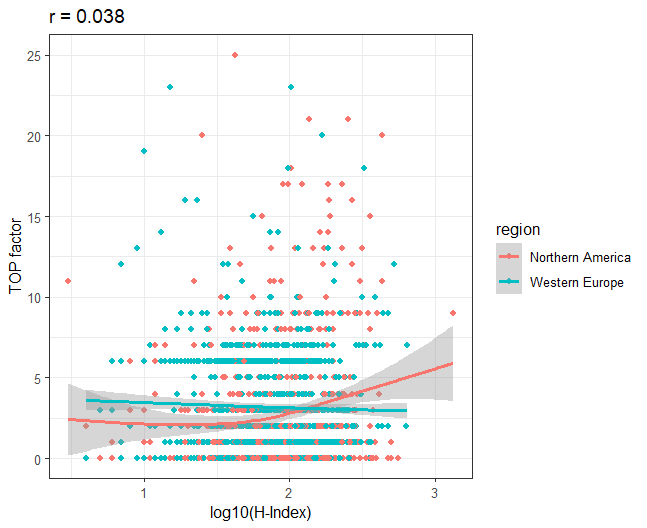
\includegraphics{images/tophindex.png}

\end{tcolorbox}

Um aus Zitationszahlen Qualität schließen zu können, wurde von Peroni
and Shotton (2012) ein System entwickelt, wie festgelegt werden kann, um
was für eine Art Zitation es sich handelt (Citation Typing Ontology,
\href{https://sparontologies.github.io/cito/current/cito.html}{CiTO})
und das bereits von Zeitschriften implementiert wurde (Willighagen
2023). Inwiefern es die Bewertung von Forschung verbessert, bleibt
abzuwarten. Nicht ganz ernstgemeint wurde für die Medizin außerdem der
Free Lunch Index vorgeschlagen, der die Summe der Geschenke aus der
Industrie abbildet (Scanff et al. 2023).

\subsection{Infrastruktur (Open
Infrastructure)}\label{infrastruktur-open-infrastructure}

In der Pyramide zum Kulturwandel bildet Infrastruktur das Fundament. Sie
ermöglicht, dass verschiedene Open Science Praktiken umgesetzt werden
können. Beispielsweise lassen sich Forschungsdaten nicht einfach
veröffentlichen, wenn es dafür keinen Ort oder keine Internetseite gibt.
Diesbezüglich gab es massive Fortschritte und Forschungsmaterialien,
Daten, oder Publikationen zu teilen war nie einfacher. Mittels der
Richtlinien für Infrastruktur in der Forschung (Bilder, Lin, and Neylon
2020) ist festgelegt, wie Infrastruktur im Idealfall aufgebaut sein
sollte: Beispielsweise sollte sie nachhaltig gestaltet und langfristig
finanziert sein und über Disziplinen, Institutionen, und Orte hinaus
verwendet werden. In Deutschland setzt sich zudem der Verein ``Nationale
Forschingsdaten Infrastruktur (NFDI) dafür ein, dass Daten als
gemeinsames Gut organisiert werden. In fachspezifischen Konsortien
werden Strukturen geschaffen, mittels derer sich Forschungsdaten teilen
lassen. Eine
\href{https://access2perspectives.org/mapping-open-science-resources/}{interaktive
Karte offener Infrastruktur} ist online verfügbar
(https://kumu.io/access2perspectives/open-science\#disciplines/by-os-principle/open-infrastructure).

\begin{tcolorbox}[enhanced jigsaw, title=\textcolor{quarto-callout-note-color}{\faInfo}\hspace{0.5em}{Die Kosten eines ``Offenen Buches''}, colbacktitle=quarto-callout-note-color!10!white, rightrule=.15mm, titlerule=0mm, left=2mm, bottomrule=.15mm, arc=.35mm, leftrule=.75mm, toprule=.15mm, opacityback=0, breakable, bottomtitle=1mm, colframe=quarto-callout-note-color-frame, toptitle=1mm, opacitybacktitle=0.6, coltitle=black, colback=white]

Dieses Buch wurde vollständig mittels kostenloser Software verfasst (GNU
R, RStudio, Quarto) und wird kostenlos bei Github gehostet. Ein weitere
Schritt wäre die ausschließliche Verwendung von Open Source Software,
also von Programemn, deren Code öffentlich gemacht wurde und welcher für
eigene Zwecke verwendet werden kann. Aktuell ist die Verfügbarkeit
dieses Buches davon abhängig, dass Github kostenlos bleibt.

\end{tcolorbox}

\begin{longtable}[]{@{}
  >{\raggedright\arraybackslash}p{(\columnwidth - 4\tabcolsep) * \real{0.2121}}
  >{\raggedright\arraybackslash}p{(\columnwidth - 4\tabcolsep) * \real{0.3603}}
  >{\raggedright\arraybackslash}p{(\columnwidth - 4\tabcolsep) * \real{0.4276}}@{}}
\caption{Beispiele für Open Science Infrastrukturen}\tabularnewline
\toprule\noalign{}
\begin{minipage}[b]{\linewidth}\raggedright
Service
\end{minipage} & \begin{minipage}[b]{\linewidth}\raggedright
Zweck
\end{minipage} & \begin{minipage}[b]{\linewidth}\raggedright
Anbieter
\end{minipage} \\
\midrule\noalign{}
\endfirsthead
\toprule\noalign{}
\begin{minipage}[b]{\linewidth}\raggedright
Service
\end{minipage} & \begin{minipage}[b]{\linewidth}\raggedright
Zweck
\end{minipage} & \begin{minipage}[b]{\linewidth}\raggedright
Anbieter
\end{minipage} \\
\midrule\noalign{}
\endhead
\bottomrule\noalign{}
\endlastfoot
Literaturdatenbank & Verwalten und Durchsuchen von Literatur &
OpenAlex \\
Datenrepositorium & Veröffentlichung von Forschungsdaten & re3data.org,
osf.io, researchbox.org, zenodo.org \\
Pre-Print Server & Veröffentlichung von Forschungsartikeln &
arXiv.org \\
Zeitschriftensystem (Editorial Manager) & Verwaltung von
wissenschaftlichen Fachzeitschriften (Einreichung, Begutachtung,
Publikation, Indizierung) & Open Journal System \\
Post-Publication Peer Review & Begutachtung und Kommentierung von
Forschung nach Veröffentlichung & Pubpeer.com \\
Identifizierung von Forschenden, Institutionen, und Forschung & & Open
Researcher and Contributor ID (ORCID.org), Research Organization
Registry (ROR.org), Digital Object Identifier (DOI.org) \\
\end{longtable}

\subsection{Open Access Publikationen}\label{sec-openaccess}

Um den Zugang zu wissenschaftlichem Wissen zu erhöhen, wird mehr und
mehr Forschung als ``Open Access'' (offener Zugang) veröffentlicht.
Spezifisch kann das auf vielen verschiedenen Wegen geschehen: Personen
können Artikel in nicht-kommerziellen Zeitschriften veröffentlichen (für
eine Sammlung an über 20.000 Zeitschriften siehe z.B. https://doaj.org),
manche kommerzielle Zeitschriften machen Artikel nach Ablauf einer
bestimmten Zeit frei verfügbar, oder sie können Geld bezahlen, damit der
Artikel öffentlich zugänglich in einer traditionellen Fachzeitschrift
erscheint. Dabei können sich die Kosten auf Werte zwischen ein paar
hunderten Euro bis zu 9.000€ bei ``angesehenen Zeitschriften'' belaufen.
Die Gelder dafür stammen meistens aus den Mitteln von Universitäten
(z.B. Open Access Funds) oder aus Projektmitteln, das heißt, dass bei
der Beantragung von Geldern für das Projekt auch Gelder mit beantragt
wurden, um die Kosten für Open Access Publikationen zu bezahlen. Während
Open Access ursprünglich explizit nicht dieses Bezahlmodell meint, haben
es Zeitschriften inzwischen ``rekommerzialisiert'', sich also zu Nutzen
gemacht. In der Open-Access-Strategie der Hochschulen des Landes
Nordrhein-Westfalen (Openness 2023b) werden die Typen übersichtlich
aufgelistet. Neben Open Access bei der Erstveröffentlichung haben
Forschende im Sinne von ``Green Open Access'' üblicherweise das Recht,
die von ihnen verfassten Artikeln auf ihrer eigenen Website, denen ihrer
Institution, oder auf fachlichen Repositorien hochzuladen. Zumstein
(2023) empfiehlt beispielsweise, bei Zeitschriften mit Abo-Modell
(``Subskriptionsmodell'') nicht die Open Access Option dazuzukaufen, da
es nicht nachhaltig ist und stattdessen die Zweitveröffentlichung offen
zu machen.

\begin{longtable}[]{@{}
  >{\raggedright\arraybackslash}p{(\columnwidth - 2\tabcolsep) * \real{0.1322}}
  >{\raggedright\arraybackslash}p{(\columnwidth - 2\tabcolsep) * \real{0.8678}}@{}}
\caption{Typen von Open Access bei der
Erstveröffentlichung}\tabularnewline
\toprule\noalign{}
\begin{minipage}[b]{\linewidth}\raggedright
Typ
\end{minipage} & \begin{minipage}[b]{\linewidth}\raggedright
Regelung
\end{minipage} \\
\midrule\noalign{}
\endfirsthead
\toprule\noalign{}
\begin{minipage}[b]{\linewidth}\raggedright
Typ
\end{minipage} & \begin{minipage}[b]{\linewidth}\raggedright
Regelung
\end{minipage} \\
\midrule\noalign{}
\endhead
\bottomrule\noalign{}
\endlastfoot
Gold / Diamond & Alle Publikationen sind sofort und kostenlos
verfügbar \\
Hybrid & Die Zeitschrift hat ein Abo-Modell. Einzelne Artikel werden
gegen eine Gebühr öffentlich gemacht. \\
Moving Wall & Die Zeitschrift hat ein Abo-Modell. Nach Ablauf einer
Frist (6-48 Monate) sind Artikel frei zugänglich. \\
Promotional & Zur Bewerbung der Zeitschrift sind einzelne Artikel frei
verfügbar. \\
\end{longtable}

Typen von Open Access (siehe zenodo NRW AG Open Science Auflistung)

\begin{tcolorbox}[enhanced jigsaw, title=\textcolor{quarto-callout-caution-color}{\faFire}\hspace{0.5em}{Wie Prestige für Offenheit blind machen kann}, colbacktitle=quarto-callout-caution-color!10!white, rightrule=.15mm, titlerule=0mm, left=2mm, bottomrule=.15mm, arc=.35mm, leftrule=.75mm, toprule=.15mm, opacityback=0, breakable, bottomtitle=1mm, colframe=quarto-callout-caution-color-frame, toptitle=1mm, opacitybacktitle=0.6, coltitle=black, colback=white]

An manchen Orten gibt es ungeschriebene Gesetze wie ``wenn du während
deiner Promotion in einer hochrangigen Zeitschrift publizierst, wirst du
die Bestnote kriegen''. Damit wird den prestigereichen Zeitschriften
immer mehr Macht zugeschoben. Leuten wird außerordentlich dafür
gratuliert, dass sie etwas in Psychological Bulletin oder sogar Nature
Human Behavior veröffentlicht haben. Dass niemand, der nicht mit einer
Universität affiliiert ist (also an einer arbeitet oder studiert), den
Artikel im Psychological Bulletin lesen kann, oder dass für die
Veröffentlichung in Nature bis zu 9.000 Euro (meistens aus
Steuergeldern) bezahlt wurden, spielt dabei keine Rolle.

\end{tcolorbox}

Neben kommerziellen und Open Access Zeitschriften existiert noch ein
weiterer Akteur bei der Zugänglichkeit von wissenschaftlichem Wissen:
Mittels \emph{Schattenbibliotheken} wie Sci-Hub können Personen auf
Artikel, die sonst hinter einer Bezahlschranke liegen, zugreifen
(``Guerilla Open Access''). Sci-Hub
(\url{https://de.wikipedia.org/wiki/Sci-Hub}) als bekannteste
Schattenbibliothek beinhaltet fast 70\% aller 81.6 Millionen
wissenschaftlichen Artikeln bis zum Jahr 2018 (Himmelstein et al. 2018).
Nutzungsstatistiken aus Deutschland hat Strecker (2019) analysiert. Die
Verbreitung und das Herunterladen sind rechtlich umstritten. Andere
Möglichkeiten, kostenlos an Forschungsartikel zu kommen sind 12ft.io,
der Hashtag \#canihazpaper in sozialen Netzwerken, oder das persönliche
Anschreiben von Autor*innen per Mail oder über soziale Netzwerke für
Forschende (Researchgate.net, Academia.edu).

\subsubsection{Wahl der Fachzeitschrift}\label{wahl-der-fachzeitschrift}

Abgesehen von Prestige oder Journal Impact Factors können Forschende bei
der Wahl der Zeitschrift, in der sie ihre Forschung veröffentlichen
möchten, auf Gold Open Access achten (z.B. via \url{https://doaj.org}
oder \url{https://freejournals.org/current-member-journals/}) und den
TOP Faktor berücksichtigen (topfactor.org). Zudem sollten sie bei ihren
Bibliotheken nachhaken: Bei Zeitschriften mit Abo-Modell (hybrid Open
Access) hat sich nämlich ein Markt für bezahlte Open Access
Publikationen entwickelt. Zeitschriften und Verlage veröffentlichen
dabei extrem viele Artikel ohne strenge Begutachtung und verdienen Geld
durch die Open Access Gebühren. In dem Fall sind die Zeitschriften als
``Open Access Zeitschriften'' vermarktet und die Kosten heißen ``Author
Processing Charges (APCs)''. Mittels des von der Universität Bielefeld
betriebenen Dashboards wird aufgeschlüsselt, welche Zeitschriften und
welche Verlage wie viel Geld von deutschen Universitäten bekommen haben
(https://treemaps.openapc.net/apcdata/openapc/\#publisher/). Der Verlag
MDPI, mit über 2000 Artikeln auf Platz 1 bei der Artikelanzahl und mit
Einnahmen von über 4 Millionen Euro auf Platz 2 hinsichtlich Profit, ist
dabei besonders umstritten: Forschende
(https://predatoryjournals.org/news/f/is-mdpi-a-predatory-publisher)
konnten Nachweisen, dass die Bearbeitungszeiten (Dauer der Begutachtung,
Revision, Veröffentlichung) unrealistisch gleichförmig sind und es pro
Tag mehrere Spezialausgaben gibt (für gewöhnlich hat eine Zeitschrift
1-2 Spezialausgaben pro Jahr). Beall hat auf seiner Website
(https://beallslist.net) eine umstrittene Liste veröffentlicht, die
Zeitschriften als unwissenschaftlich kennzeichnet und beschreibt seine
Erfahrungen in einem Artikel (Beall 2017). Ebenfalls helfen Tools zur
Identifikation unseriöser Zeitschriften und Konferenzen
(\hyperref[0]{https://thinkchecksubmit.org},
\hyperref[0]{https://thinkcheckattend.org}).

\subsubsection{Monitoring}\label{monitoring}

Wie viel Forschung als Open Access veröffentlicht wird oder wie viel das
Kostet, lässt sich mithilfe verschiedener Werkzeuge beobachten.
\emph{OpenAPCs} listet Open Access Kosten je nach Verlag, Zeitschrift,
und Universität auf (https://treemaps.openapc.net/apcdata/openapc/) und
der Open Access Monitor schlüsselt auf, wie viele Publikationen in
Deutschland unter welchen Open Access Modellen veröffentlicht werden
(\url{https://open-access-monitor.de}).

Aktuell (Stand Sommer 2024) haben 54,4\% aller indizierten
Fachzeitschriften kein offenes Modell und der Großteil aller Forschung
wird darüber veröffentlicht. 19,2\% der Fachzeitschriften laufen
außerdem unter einem Transformationsvertrag. Dabei soll ein Übergang vom
Abo-Modell zu einem Open Access Modell geschafft werden und alle bisher
veröffentlichten Artikel sollen ebenfalls öffentlich zugänglich gemacht
werden. Die wohl größte Rolle spielt dabei das DEAL Konsortium
(\url{https://deal-konsortium.de/publizierende}): Dabei haben sich
deutsche Wissenschaftsorganisationen zusammengeschlossen, um mit
Verlagen einen bundesweiten Vertrag auszuhandeln, das allen deutschen
Forschenden ermöglicht, Open Access ohne zusätzliche Kosten zu
publizieren.

\begin{tcolorbox}[enhanced jigsaw, title=\textcolor{quarto-callout-note-color}{\faInfo}\hspace{0.5em}{Offene Lehrbücher}, colbacktitle=quarto-callout-note-color!10!white, rightrule=.15mm, titlerule=0mm, left=2mm, bottomrule=.15mm, arc=.35mm, leftrule=.75mm, toprule=.15mm, opacityback=0, breakable, bottomtitle=1mm, colframe=quarto-callout-note-color-frame, toptitle=1mm, opacitybacktitle=0.6, coltitle=black, colback=white]

Während Artikel in Fachzeitschriften primär für den Austausch unter
Forschenden genutzt werden, spielen Lehrbücher die besondere Rolle, dass
sie die Kommunikation zwischen Expert*innen und Interessierten (z.B.
Studierenden) bilden. Das Verhältnis zwischen Lehrbuch-Autor*innen und
Verlagen ist weniger angespannt als das zwischen Forschenden und
Zeitschriften - auch, wenn es größtenteils dieselben Verlage sind. Zwei
besondere Unterschiede könnten die Ursache dafür sein: 1.
Verfasser*innen von Lehrbüchern verdienen von Verkäufen und 2. können
sie ihre eigenen Werke für Prüfungen relevant erklären. In der Folge
müssen Studierende die Kosten tragen und nicht sie selbst. Im
Vereinigten Königreich existieren bereits Pilotprojekte, die das Ziel
haben, die Lehre möglichst vollständig auf offene Lehrbücher umzustellen
(Farrow, Pitt, and Weller 2020).

\end{tcolorbox}

\subsubsection{Massenrücktritte von
Herausgeber*innen}\label{massenruxfccktritte-von-herausgeberinnen}

Immer häufiger kommt es vor, dass die Herausgeberschaft einer
Zeitschrift zurücktritt. Grund dafür, dass Verlage die
Publikationskosten oder die Anzahl veröffentlichter Artikel erhöhen
möchte. Eine Liste solcher Rücktritte verwaltet Retractionwatch.org
(``Editorial Mass Resignations'',
https://retractionwatch.com/the-retraction-watch-mass-resignations-list/).
Dabei hat eine Community aus Forschenden jahrelang hart gearbeitet, um
die Zeitschrift zu verwalten und bekannt zu machen und wird dann damit
bestraft, dass sie noch mehr Geld dafür zahlen muss, ihre Forschung
miteinander auszutauschen.

In vielen solcher Fälle gründen die Forschenden im Anschluss an ihren
Rücktritt eine neue, üblicherweise Open Access Zeitschrift. Während
Universitätsbibliotheken Gründungen neuer Zeitschriften unterstützen und
der Prozess technisch unproblematisch ist, gibt es legale und soziale
Hürden: Verlage wie Taylor \& Francis vereinbaren mit den Forschenden
häufig ``Non-comepete Klauseln'', verbieten ihnen also, im Anschluss an
ihre Herausgebertätigkeit innerhalb eines oder mehrerer Jahre bei einer
anderen Zeitschrift zu arbeiten. Eine wissenschaftliche Community, die
der
\href{https://blogs.lse.ac.uk/impactofsocialsciences/2019/03/29/the-value-of-a-journal-is-the-community-it-creates-not-the-papers-it-publishes/}{Kern}
einer Zeitschrift ist, muss außerdem einstimmig hinter der Veränderung
stehen. In einem Fall hat die Herausgeberschaft klar kommuniziert, dass
es sozial völlig inakzeptabel ist, die alte Zeitschrift zu unterstützen.
Neu gegründete Zeitschriften haben außerdem noch keinen Impact Factor,
weil noch keine zitierfähigen Artikel erschienen sind und Artikel noch
nicht zitiert werden konnten. Verlage arbeiten gegen Massenrücktritte,
indem sie die Zugehörigen der Herausgeberschaft häufig rotieren, sodass
sie sich schlechter absprechen können. Treffen in Person sind durch die
Internationalität der Forschung ebenfalls erschwert.

\begin{tcolorbox}[enhanced jigsaw, title=\textcolor{quarto-callout-note-color}{\faInfo}\hspace{0.5em}{Offenheit durch Klemmbausteine}, colbacktitle=quarto-callout-note-color!10!white, rightrule=.15mm, titlerule=0mm, left=2mm, bottomrule=.15mm, arc=.35mm, leftrule=.75mm, toprule=.15mm, opacityback=0, breakable, bottomtitle=1mm, colframe=quarto-callout-note-color-frame, toptitle=1mm, opacitybacktitle=0.6, coltitle=black, colback=white]

Offenheit der Wissenschaft kann viele Gesichter haben: Eine besondere
Form des öffentlichen Zugangs verbreitet sich aktuell in der
biotechnologischen Forschung aus. Damit Wissenschaftler*innen,
Ingenieur*innen, aber auch die allgemeine Bevölkerung Zugang zu
Konstruktionen hat, wird dort zu Klemmbausteinen wie beispielsweise
solchen von dem Unternehmen LEGO® gegriffen (Boulter et al. 2022). Das
Patent für ``den Lego-Stein'' ist bereits ausgelaufen, sodass
verschiedene Unternehmen oder Personen mit 3D-Drucker eigene
Klemmbausteine herstellen können. Die Dateien für 3D-Drucker sind im
Internet frei verfügbar. So konnte der Forscher David Aguilar
beispielsweise einen prosthetischen Arm mit Klemmbausteinen entwerfen.

\end{tcolorbox}

\subsection{Pre-Prints}\label{pre-prints}

Wie bereits im Kapitel zur Begutachtung von Pre-Prints erläutert, sind
Pre-Prints immer öffentlich und kostenlos verfügbar. Forschende können
verschiedene Lizenzen vergeben, die beispielsweise eine kommerzielle
Verwendung verbietet, sind dabei jedoch fast immer sehr liberal. Neben
den bereits diskutierten Vorteilen von Pre-Prints, sind Änderungen bei
ihnen um ein vielfaches schneller: Forschende können jederzeit auf
Kritik reagieren und Fehler korrigieren. In einem
\href{https://www.statnews.com/2020/02/03/retraction-faulty-coronavirus-paper-good-moment-for-science/}{Artikel
zum Coronavirus} fiel ein Fehler kurz nach der Veröffentlichung auf und
wurde innerhalb von zwei Tagen korrigiert. Bei einem
Zeitschriftenartikel kann sich dieser Prozess über viele Jahre ziehen.
Gerade bei ernsthaften Problemen, die eine Retraction zur Folge haben,
sind Verlage vergleichsweise langsam. Einen Pre-Print können Autor*innen
jederzeit vom Netz nehmen - wobei er über Suchmaschinen dabei sicherlich
noch auffindbar bleibt.

Pre-Prints können außerdem dazu beitragen, dass Ressourcen effizienter
benutzt werden: Durch die beschleunigte Kommunikation zwischen
Forschenden fällt schneller auf, wenn verschiedene Gruppen an derselben
Fragestellung arbeiten. So können sich Kooperationen bilden oder Gruppen
verlagern ihre Schwerpunkte.

\begin{tcolorbox}[enhanced jigsaw, title=\textcolor{quarto-callout-note-color}{\faInfo}\hspace{0.5em}{Unberechtigte Sorge vor Ideenklau}, colbacktitle=quarto-callout-note-color!10!white, rightrule=.15mm, titlerule=0mm, left=2mm, bottomrule=.15mm, arc=.35mm, leftrule=.75mm, toprule=.15mm, opacityback=0, breakable, bottomtitle=1mm, colframe=quarto-callout-note-color-frame, toptitle=1mm, opacitybacktitle=0.6, coltitle=black, colback=white]

In manchen wissenschaftlichen Disziplinen sind Forschende Pre-Prints
gegenüber zögerlich. Sie haben Angst, dass jemand ihre Idee klaut und
schneller als sie einen Artikel bei einer Fachzeitschrift dazu
veröffentlicht. Während diese Angst beim klassischen System z.B. durch
böswillige Gutachtende oder Zuhörer*innen bei einer Konferenz ebenfalls
besteht und selbst bei veröffentlichten Fachzeitschriftenartikeln
passiert, ist der Vorteil von Pre-Prints, dass sie mit einem Datum
versehen sind und für alle klar nachvollziehbar ist, wann was
veröffentlicht wurde.

\end{tcolorbox}

\subsection{Ansätze gegen die Selektion spannender
Ergebnisse}\label{ansuxe4tze-gegen-die-selektion-spannender-ergebnisse}

Die Ergebnisse einer Untersuchung sind das, was am wenigsten in der Hand
der forschenden Person liegt (bzw. liegen sollte - immerhin interessiert
uns ja die Wahrheit und nicht die Kompetenz Forschender, Daten möglichst
stark zu schönen). Umso frustrierender ist es, dass Zeitschriften das
Ergebnis als Kriterium zur Publikation verwenden. Unter der Vielzahl von
Einreichungen werden vor allem diejenigen Artikel gewählt, die spannende
Ergebnisse erzielt haben oder die ihre anfängliche Vermutung bestätigen
konnten (\emph{Confirmation Bias}). Die folgenden Ansätze lösen dieses
Problem zum Beispiel dadurch, dass die Ergebnisse aus dem
Begutachtungsprozess ausgeschlossen werden.

\subsubsection{Results-blind peer
review}\label{results-blind-peer-review}

Der einfachste Weg ist dabei, den Ergebnisteil einfach zu schwärzen oder
wegzulassen. Verschiedene Zeitschriften bieten das als Option an. Da es
sich hierbei zurzeit (2024) eher um eine Ausnahme handelt, ist den
meisten Gutachtenden jedoch klar, dass vor allem diejenigen die Option
zum results-blind peer review wählen, deren Ergebnisse nicht ``hübsch
genug'' für den klassischen Weg sind.

\subsubsection{Registered Report}\label{registered-report}

\begin{figure}[H]

{\centering 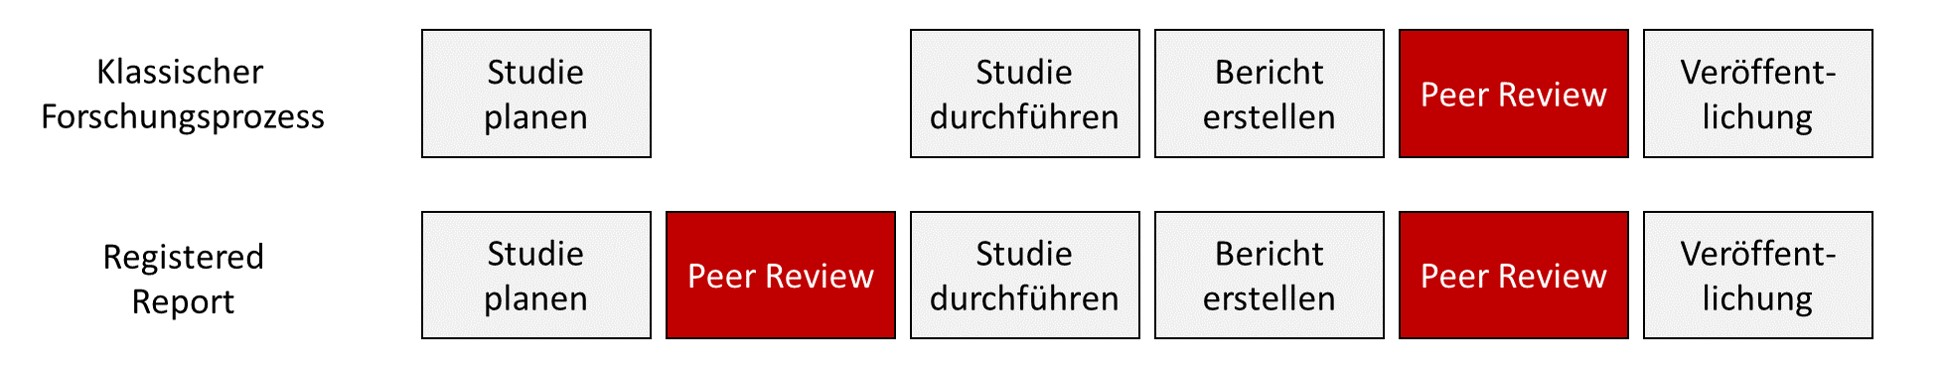
\includegraphics{images/peerreview.jpg}

}

\caption{Klassischer Forschungsprozess im Vergleich zu Registered
Reports mit zusätzlicher Begutachtung vor der Studiendurchführung}

\end{figure}%

Ein radikalerer Ansatz als die Begutachtung ohne Ergebnisteil ist die
Begutachtung des Artikels, ohne dass Ergebnisse überhaupt existieren.
Dieses Format heißt \emph{Registered Report}. Dabei wird das Manuskript
mit der zu prüfenden Theorie, Methodik, und dem Analyseplan bei der
Zeitschrift eingereicht, ohne dass überhaupt Daten erhoben wurden. Kommt
es zur Akzeptanz dieses „halbfertigen'' Artikels (\emph{in principle
acceptance}), werden die Daten gesammelt, wie geplant ausgewertet, und
es folgt eine weitere Begutachtungsrunde. Hierbei ist vorgeschrieben,
dass die Autor*innen nichts an den bereits verfassten Teilen verändern
dürfen und die Gutachter*innen im Nachhinein keine Kritik am bereits
geprüften Vorgehen üben dürfen. Es geht nur noch darum, ob der Plan
eingehalten wurde und ob die Schlussfolgerungen auf den geplanten
Analysen fußen. Damit soll verhindert werden, dass Artikel abgelehnt
werden, weil die Ergebnisse nicht spannend genug, innovativ genug, oder
den Erwartungen entsprechend sind. Erste Untersuchungen können bereits
nachweisen, dass sich damit die Qualität der Forschung gegenüber dem
traditionellen Vorgehen verbessert (Soderberg et al. 2021). Eine
Übersicht über Zeitschriften, die dieses Format anbieten ist online
verfügbar (\url{https://www.cos.io/initiatives/registered-reports} à
Participating Journals; (\textbf{Chambers?}).; C. D. Chambers and
Tzavella (2022)).~ Ebenfalls wird dadurch deutlich, dass Forschung einem
massiven Publikationsbias unterliegt (d.h. es werden vor allem Studien
veröffentlicht, die ihre Vermutungen bestätigen konnten und kaum
Studien, in denen das nicht geschah): (\textbf{Scheel2021?}) zeigten,
dass der Anteil erwartungskonformer Ergebnisse bei Registered Reports
mit 44\% deutlich unter den in der Psychologie üblichen 96\% liegt.

\subsubsection{Pre-Print basierte
Modelle}\label{pre-print-basierte-modelle}

Durch die immer häufigere Veröffentlichung von Pre-Prints, also noch
nicht begutachteten Manuskripten, eröffnen sich für die Begutachtung
neue Wege. Sogenannte Overlay Journals (elife) wählen unter Pre-Prints
solche aus, die sie an Gutachtende schicken um deren Meinungen
einzuholen. Sofern die Autor*innen des Preprints einverstanden sind,
erhalten sie dann Gutachten und ihr Artikel wird schließlich in der
Zeitschrift veröffentlicht.

Je nach Fach haben unterschiedlich viele Zeitschriften mit PCI
Initiativen Vereinbarungen, dass sie die akzeptierten Artikel ohne
eigenes Peer Review veröffentlichen. Mehr und vor allem bekannte
teilnehmende Zeitschriften machen PCIs für Forschende attraktiver.
Zeitschriften, die Interesse an einem PCI haben, aber die Begutachtung
nicht aus der Hand geben möchten, können sich als „PCI interested
Journals'' listen lassen (vs.~„PCI friendly journals''). Teilnehmende
Zeitschriften sparen dadurch Arbeit und bleiben relevant, indem sich
Ihre Funktion dahin verschiebt, dass sie thematisch relevante Forschung
sammeln und disseminieren. In einem Fall hat bereits eine Zeitschrift,
die als „PCI friendly'' eine Vereinbarung mit PCI-RR hatte, ein
Manuskript mit einer \emph{Recommendation} zum erneuten Peer Review
versendet und wurde sofort von den PCI Partnern entfernt. Forschende,
die Gutachtenprozesse für PCIs organisieren möchten -- analog zu
Herausgeber*innen von klassischen Zeitschriften -- können
\emph{Recommender} werden und müssen dazu ein Mindestmaß an Wissen haben
sowie eine Schulung absolvieren
(\url{https://rr.peercommunityin.org/about/recommenders}).

\textbf{Tabelle 2}

\emph{Zusammenfassung der verschiedenen Begutachtungsmodelle und der
jeweiligen Art des Umgangs mit den Forschungsergebnissen}

\begin{longtable}[]{@{}
  >{\raggedright\arraybackslash}p{(\columnwidth - 2\tabcolsep) * \real{0.3966}}
  >{\raggedright\arraybackslash}p{(\columnwidth - 2\tabcolsep) * \real{0.6034}}@{}}
\toprule\noalign{}
\endhead
\bottomrule\noalign{}
\endlastfoot
\textbf{Begutachtungsprozedur} & \textbf{Ausblendung der Ergebnisse} \\
Traditionell & Ergebnisse sind sichtbar und fließen in die Beurteilung
ein \\
Results-Blind Peer Review & Ergebnisse liegen vor, werden den
Begutachtenden jedoch vorenthalten \\
Registered Report & Ergebnisse liegen noch nicht vor \\
Peer-Community-In Registered Report (PCI-RR) & Ergebnisse liegen noch
nicht vor \\
\end{longtable}

\begin{tcolorbox}[enhanced jigsaw, title=\textcolor{quarto-callout-note-color}{\faInfo}\hspace{0.5em}{Anekdoten: Meine schlimmsten Erfahrungen mit Peer Review}, colbacktitle=quarto-callout-note-color!10!white, rightrule=.15mm, titlerule=0mm, left=2mm, bottomrule=.15mm, arc=.35mm, leftrule=.75mm, toprule=.15mm, opacityback=0, breakable, bottomtitle=1mm, colframe=quarto-callout-note-color-frame, toptitle=1mm, opacitybacktitle=0.6, coltitle=black, colback=white]

Peer Review ist brutal. Das ist meine persönliche Erfahrung mit dem
Prozess. Früh musste ich in meiner wissenschaftlichen Arbeit lernen,
dass es in vielen Fällen ein Glücksspiel ist. Renommierte
Wissenschaftler*innen erklärten mir, dass sie Artikel hätten, die sie
über Jahre immer wieder bei Zeitschriften immer wieder eingereicht
hätten, und die schließlich positiv aufgenommen worden wären, ohne, dass
sie sie stark verändert hätten. Jenseits von der Akzeptanz eines
Artikels zur Publikation geht es auch um die Gründe für die Ablehnung:
Häufig lesen Gutachtende Artikel nicht aufmerksam und Kritiken sind
nicht konstruktiv. Hierzu meine schlimmsten Erfahrungsberichte.

\textbf{Einreichung bei Collabra}: Es handelte sich um einen Artikel,
der zwischen den Disziplinen steht. Es geht nicht nur um Erwartungen,
nicht nur um Produktbewertungen, nicht nur um die Methode, Daten direkt
aus dem Internet herunterzuladen. Der ``bunte-Vogel-Artikel'' war
bereits bei drei Zeitschriften abgelehnt worden. Bei keiner wurde er an
die Reviewer weitergegeben, weil er nie zur Zeitschrift passte. Die
Zeitschrift \emph{Collabra}, bei der wir ihn schließlich einreichten,
war zu dem Zeitpunkt noch wenige Jahre alt und war breit aufgestellt.
Nach der Einreichung im Mai 2020 haben wir über ein halbes Jahr lang auf
das Gutachten gewartet. Länger zu warten ist erstmal ein gutes Zeichen:
Der Artikel wurde wohl an Reviewer rausgeschickt. In dem Fall wurden wir
jedoch bitter enttäuscht: Im November 2020 erfuhren wir auf Nachfrage
hin, dass 14 Gutachter*innen angefragt wurden, sodass die Herausgeberin
auf Basis eines Gutachtens entschied, das Manuskript abzulehnen. Grund
dafür war, dass die Methode aufgrund der inzidentellen Daten nicht
geeignet für die Fragestellung war. In der Psychologie sowie den
Wirtschaftswissenschaften ist das Problem mit ``echten Daten'' seit
mehreren Jahrzehnten bekannt und wir hatten es bereits ausgiebig im
Artikel diskutiert.

\textbf{Einreichung bei Journal of Experimental Social Psychology}: Wir
hatten eine Replikation einer dort erschienen Studie durchgeführt - der
Befund ließ sich nicht replizieren. Meine Überlegung war, der
Zeitschrift, die den nicht robusten Befund ursprünglich publizierte,
selbst die Chance zur Selbstkorrektur zu geben. Die Reviews waren fair
und positiv, es gab ein paar Punkte zu diskutieren, aber uns war klar,
dass es sich hier um Verständnisprobleme und keine inhaltlichen Aspekte
handelte. Nicht so der Editor: Er erklärte, dass der Befund nicht neu
genug wäre und klar wäre, dass es nicht replizierbar ist. Ich erklärte
ihm, dass noch niemand den Befund zu replizieren versucht hatte und wir
selbst sogar vor der Analyse der Ergebnisse eine Abstimmung darüber
gemacht hatten, welches Ergebnis wir erwarteten: Es war sehr ausgewogen
50-50. Darüber hinaus, wurde ein weiterer Artikel publiziert, der
entgegengesetzt Ergebnisse hatte. Wir stellten klar, dass wir alle
aufgezeigten Probleme einfach lösen können und gerne die Chance zur
Revidierung hätten. Der Editor hätte dabei kaum Arbeit außer den Artikel
anschließend nochmal an Gutachtende zu schicken. Auf unsere Mail
erhielten wir nur eine kurze Antwort: \emph{Hi. I know my decision is
disappointing, but I'm going to stick with my decision on this one.}
Hier befand ich mich an einem Scheideweg: Warum ist ein Forscher nicht
bereit, Gründe für eine wissenschaftliche Entscheidung zu erörtern? Wir
entschieden uns, einen anderen Editor direkt zu kontaktieren. Nach
kurzer Zeit erhielten wir die Einladung zu einer Revision. Der Artikel
wurde schließlich in der revidierten Fassung veröffentlicht.

\textbf{Einreichung bei European Journal of Personality}: Die zentrale
Aussage dieses Artikel war, dass verschiedene Messwerte einer
angeblichen Eigenschaft nicht miteinander zusammenhängen. Der Befund
stellte die Annahme infrage, dass es sich dabei überhaupt um eine
Eigenschaft handelte. Die Ablehnungsgründe zweier Gutachtenden und der
Herausgeberin machten deutlich: Niemand hatte den Artikel überhaupt
gelesen. Ein Gutachter merkte an, dass etwas mit den Werten nicht
stimme, weil sie laut einer der Tabellen nicht miteinander
zusammenhängen. Genau das war ja unsere Aussage. Wir zeigten, dass es
nich an unseren Daten lag, sondern sich in anderen Datensätzen so
verhielt. Hätte er die Überschrift der Tabelle gelesen, den Absatz
davor, oder den danach, wäre das klar geworden. Hat er aber
nicht\ldots{}

Das sind nur kurze Auszüge aus dutzenden Einreichungen und Ablehnungen.
Darüber hinaus kann fast jede*r Forschende*r von substanzlosen
persönliche Beleidigungen berichten. Meiner Erfahrung nach ist anonymes
versus öffentliches Peer Review wie ein Vergleich von anonymen
Kommentarspalten mit nicht anonymen: Bei Anonymität beherrschen
persönliche Beleidigungen und Unwahrheiten den Dialog.

\end{tcolorbox}

\subsection{Replikationsforschung}\label{replikationsforschung}

Häufig ist die Rede von einer Replikationskrise, also einer Krise von zu
geringer Replizierbarkeit. Wenig überraschend hat sich das auf die Rolle
von Replikationen in den Sozialwissenschaften und darüber hinaus
ausgewirkt. Zahlreiche Wege wurden eingeschlagen, die das Ansehen von
Replikationsstudien und damit ihre Häufigkeit in der Forschung erhöhen.
Dabei müssen die Wissenschaften nachholen, was sie zu Beginn ihrer
Existenz hätten tun sollen, nämlich festzulegen, welche Ansprüche an
Replizierbarkeit bestehen und wie diese geprüft werden sollen. Mit
Replizierbarkeit meine ich dabei, dass eine Hypothese sich auch mit
anderen Daten als denen der Originalstudie bestätigen lässt. Es geht
also um ein minimales Maß an Verallgemeinerbarkeit und nicht primär um
ein tieferes Verständnis von Theorien, auch, wenn letzteres dennoch
manchmal kritisiert wird, obwohl niemand behauptet hat, Replikationen
sollten das Theorie-Problem ebenfalls lösen (Feest 2019).

\begin{tcolorbox}[enhanced jigsaw, title=\textcolor{quarto-callout-note-color}{\faInfo}\hspace{0.5em}{Unschärfe von Replikationsstudien}, colbacktitle=quarto-callout-note-color!10!white, rightrule=.15mm, titlerule=0mm, left=2mm, bottomrule=.15mm, arc=.35mm, leftrule=.75mm, toprule=.15mm, opacityback=0, breakable, bottomtitle=1mm, colframe=quarto-callout-note-color-frame, toptitle=1mm, opacitybacktitle=0.6, coltitle=black, colback=white]

Ein noch ungelöstes Problem ist die Unschärfe von Original- \emph{und}
Replikationsstudien. Ting and Greenland (2024) kritisieren, dass die
Ungenauigkeit von Replikationsstudien oft missachtet wird. Ihnen entgeht
dabei jedoch, dass Replikationsstudien in fast allen Fällen eine weitaus
höhere Schärfe im Studiendesign haben und höhere methodische Standards
einhalten, als alle vorherigen Studien. Schönigung von Ergebnissen im
Sinne von p-hacking (Simmons, Nelson, and Simonsohn 2011) sind
prinzipiell auch bei Replikationen möglich (Protzko 2018), durch die
höheren Standards jedoch schwieriger. Zwar berücksichtigen Forschende
Replikationsbefunde in ihren Urteilen angemessen (McDiarmid et al.
2021), Untersuchungen dazu, wie Anfällig Replikationen für
Datenfälschung im Vergleich zu Originalstudien sind, gibt es bisher noch
keine.

\end{tcolorbox}

\subsubsection{\texorpdfstring{Was \emph{soll} sich replizieren
lassen?}{Was soll sich replizieren lassen?}}\label{was-soll-sich-replizieren-lassen}

Vor dem Hintergrund der Robustheit wird klar, wann eine erfolgreiche
Replikation zu erwarten ist und wann nicht: Wird eine Hypothese in einer
Originalstudie als allgemeingültig formuliert (z.B. kurz nach der Geburt
wiegen männliche Babys im Mittel mehr als weibliche Babys), sollte sie
sich auch wiederholbar nachweisen lassen. Dem stehen Fälle gegenüber,
wenn eine Hypothese nicht allgemeingültig formuliert ist (z.B. dass
etwas auf einen spezifischen Kontext bezogen ist wie in qualitativer
Forschung). Es gibt ganze Disziplinen, für die Replizierbarkeit
irrelevant ist, beispielsweise wird in der Archäologie bei Ausgrabungen
ein Objekt aus seinem Kontext gerissen und damit das Original
``zerstört''. Dieser Prozess ist nicht wiederholbar und es hat auch
niemand den Anspruch daran. Ebenfalls ist es möglich Artefakte (also
Befunde, die nur durch Methoden entstanden sind) zu wiederholen, wenn
deren Ursprung auf einer allgemeinen Gesetzgültigkeit basiert (Devezer
et al. 2021). Zum Beispiel kann es vorkommen, dass ein statistisches
Modell replizierbar ``anschlägt'', also Befundmuster identifiziert, auch
wenn diese nicht auf Grund der eigentlichen Erklärung entstehen sondern
nur, weil sie schlecht kalibriert sind oder ihre Voraussetzungen
verletzt wurden. Beispielsweise schien es lange Zeit so, dass
Linkshänder*innen früher sterben als Rechtshänder*innen. Dieser Befund
konnte eine Zeit lang für verschiedene deutsche Stichproben nachgewiesen
werden und es wurden bereits Überlegungen angestellt, woran das liegen
könnte. Anhand heutiger Daten ist die Replikation nicht mehr möglich,
weil es sich um ein Artefakt handelte: Bis vor einigen Jahrzehnten
wurden alle Kinder dazu erzogen, mit rechts zu schreiben und zu
schneiden. Schließlich stoppte die Umerziehung. Um in den
darauffolgenden Jahren als linkhändrige Person in den Sterbestatistiken
aufzutauchen, musste man ziemlich jung gestorben sein - denn ältere
Personen, die mit links schreiben, gab es ja aufgrund der Umerziehung
nicht. Das hatte zur Folge, dass linkshändrige Tote im Mittel ganze 10
Jahre jünger waren als rechtshändrige Tote. Replizierbarkeit ist also
nicht hinreichend für Validität oder Wahrheit, aber um die Gültigkeit
einer Hypothese zu unterstreichen oder ihren Wahrheitsanspruch zu
verteidigen ist Replizierbarkeit notwendig.

Fletcher (2021) listet die Bedingungen dafür auf, dass sich etwas
replizieren lässt:

\begin{enumerate}
\def\labelenumi{\arabic{enumi}.}
\item
  Es liegen keine Fehler in der Datenanalyse vor.
\item
  Der Befund ist nicht auf statistische Unschärfe zurückzuführen.
\item
  Der Befund hängt nicht von vernachlässigten Hintergrundfaktoren ab.
\item
  Es lag kein Betrug oder anderes wissenschaftliches Fehlverhalten vor.
\item
  Der Befund lässt sich auf eine Grundgesamtheit verallgemeinern, die
  größer als die Stichprobe der Originalstudie ist.
\item
  Die Hypothese ist auch dann noch gültig, wenn sie auf eine völlig
  andere Weise geprüft wird.~
\end{enumerate}

\begin{tcolorbox}[enhanced jigsaw, title=\textcolor{quarto-callout-tip-color}{\faLightbulb}\hspace{0.5em}{Notwendige und hinreichende Bedingung}, colbacktitle=quarto-callout-tip-color!10!white, rightrule=.15mm, titlerule=0mm, left=2mm, bottomrule=.15mm, arc=.35mm, leftrule=.75mm, toprule=.15mm, opacityback=0, breakable, bottomtitle=1mm, colframe=quarto-callout-tip-color-frame, toptitle=1mm, opacitybacktitle=0.6, coltitle=black, colback=white]

Replizierbarkeit ist eine notwendige aber keine hinreichende Bedingung
für Allgemeingültigkeit, was ist damit gemeint? Die Begriffe
``notwendig'' und ``hinreichend'' sind vielen Personen wahrscheinlich
aus der mathematischen Kurvendiskussion bekannt. Ihre genaue Bedeutung
ist vor allem in der Logik relevant:

\begin{itemize}
\item
  Notwendig heißt ``es geht nicht ohne''. Kakaopulver zu haben, ist
  notwendig dafür, dass ich einen Kakao zubereiten kann heißt, ich kann
  keinen Kakao zubereiten, wenn ich kein Kakaopulver habe. Gleichzeitig
  ist es nicht ausreichend oder hinreichend: Nur, weil ich Kakaopulver
  habe, heißt das nicht, dass ich Kakao zubereiten kann. Vielleicht
  fehlt noch Milch, Wasser, eine Tasse, oder eine Mikrowelle.
\item
  Hinreichend heißt: Wenn es da ist, dann reicht das schon und keine
  weiteren Bedingungen müssen erfüllt sein. Wenn ich ein Flugzeug am
  Himmel höre, dann ist das hinreichend dafür, dass am Himmel ein
  Flugzeug entlang fliegt. Es ist aber auch möglich, dass ein Flugzeug
  am Himmel entlang fliegt, ohne dass ich es höre (zum Beispiel, weil es
  sehr hoch fliegt, die Umgebungsgeräusche sehr laut sind, oder es ein
  leiser Segelflieger ist).
\end{itemize}

Anders als in manchen Beispielen, muss die Bedingung nicht immer vor dem
Ereignis auftreten. Es geht also um keinen Kausalzusammenhang, bei dem
eines zum anderen \emph{führt}. Eine Besonderheit bei Bedingungen ist,
dass wenn A notwendig für B ist, dann ist B hinreichend für A. Dass ich
einen Kakao zubereitet habe, ist also hinreichend dafür, dass ich
Kakaopulver habe. Und, dass ein Flugzeug am Himmel entlang fliegt ist
notwendig dafür, dass ich es hören kann.

\end{tcolorbox}

\subsubsection{Wer repliziert?}\label{wer-repliziert}

Trotz starker Bemühungen sind Replikationsstudien immer noch relativ
selten. Schätzungen reichen von 5\% bis unter 0.1\% je nach
Forschungsdisziplin.

\begin{itemize}
\item
  Niemand repliziert

  \begin{itemize}
  \item
    \url{https://www.econstor.eu/bitstream/10419/267931/1/I4R-DP013.pdf}
  \item
    \url{https://osf.io/preprints/psyarxiv/fzngs}
  \item
    \url{https://journals.sagepub.com/doi/10.1177/1745691620979806}
  \item
    \url{https://peerj.com/articles/7654/}
  \item
    \url{https://doi.org/10.1016/j.respol.2018.07.019}
  \item
    \url{https://doi.org/10.1111/lang.12286}
  \item
    \url{https://journals.sagepub.com/doi/10.1177/0741932516646083}
  \item
    \url{https://journals.sagepub.com/doi/10.1177/1477370815578197}
  \item
    \url{https://journals.sagepub.com/doi/10.3102/0013189X14545513}
  \item
    \url{https://journals.sagepub.com/doi/10.1177/1745691612460688}
  \item
    \url{https://www.journals.uchicago.edu/doi/10.1086/506236}
  \item
    \url{https://osf.io/preprints/psyarxiv/sa6rc}
  \item
    \url{https://www.pnas.org/doi/abs/10.1073/pnas.2208863120}
  \item
    tweet von
    gilad:~https://twitter.com/giladfeldman/status/1735950123291779119
  \end{itemize}
\end{itemize}

\subsubsection{Ansehen von
Replikationsstudien}\label{ansehen-von-replikationsstudien}

Replikationen von Bem's berüchtigter Studie zum Erfühlen der Zukunft
wurden bei der Zeitschrift, bei der sie veröffentlicht wurde, ohne
Begutachtungsprozess abgelehnt (``Desk Reject''). Der Editor erklärte,
die Zeitschrift veröffentlicht keine Replikationsstudien, egal was dabei
herauskam, da sie nicht die Zeitschrift der Bem Replikationen sein
möchten (Daniel Lakens 2023). Unter den 3185 Zeitschriften mit TOP
Faktor gaben im Jahr 2024 341 Zeitschriften (10.7\%) an, dass sie
Replikationen akzeptieren. Sie werden als Konfrontation der aktuellen
theoretischen Erwartungen mit aktuellen Daten definiert und ihre
wichtige Rolle im wissenschaftlichen Prozess mehr und mehr anerkannt
(REF
\url{https://journals.plos.org/plosbiology/article?id=10.1371/journal.pbio.3000691}).
Ein Großteil dieser Entwicklung ist von der Sozialpsychologie getragen,
andere Felder verändern sich kaum oder nur langsam (REF,
\url{https://psycharchives.org/en/item/74463c10-7347-4bf2-8156-5618d42c4e93}),
doch selbst dort sind Diskussionen von Replikationsbefunden zum Teil
noch hart und die Replikationen werden (REF,
\hyperref[0]{https://osf.io/96pnj}).

In den Wirtschaftswissenschaften hat sich das Insitute for Replications
(I4R, \url{https://i4replication.org/reports.html}) gebildet, welches
sogenannte Replication Games organisiert, bei denen Studien reproduziert
und repliziert wurden. Anknüpfend an eine Forderung (Zimmermann 2015)
wurde das Journal of Comments and Replications in Economics (JCRe)
gegründet. Ab 2024 konzentriert sich das I4R darauf, Replikationen zu
spezifischen Zeitschriften durchzuführen. Ironischerweise tut es das
nicht für Open Access Zeitschriften, sondern beispielsweise für Nature
(REF \url{https://www.nature.com/articles/s41562-023-01807-2}).

\subsubsection{Arten von
Replikationsprojekten}\label{arten-von-replikationsprojekten}

Während ein Großteil der Replikationsstudien klassischen Studien
entspricht, haben sich Spezialmodelle entwickelt. Beispielsweise können
Forschende mit StudySwap Gruppen suchen, die ihre Ergebnisse vor der
Veröffentlichung replizieren (REF
\url{https://osf.io/preprints/psyarxiv/dtvs7/}; p.~11). Im Rahmen von
Registered Replication Reports konzentrieren sich große Teams an
mehreren Orten auf eine zuvor abgestimmte Studie und führen sie
gleichzeitig überall durch. Einer der fruchtbarsten Ansätze ist die
Nutzung von Abschlussarbeiten für Replikationen. Im Rahmen eines
Studiums müssen alle Studierende eine Abschlussarbeit (z.B.
Bachelorarbeit oder Masterarbeit) ablegen. Anhand von Replikationen
können sie lernen, eine wichtige Studie nachzubilden und prüfen
gleichzeitig die Robustheit der Originalbefunde. Während Quintana (2021)
vorschlug, Abschlussarbeiten so zu verwenden, ist es bereits gängige
Praxis in den vergleichenden Politikwissenschaften (Korell, Reinecke,
and Lott 2023b), in der Psychologie (Jekel et al. 2020; Feldman 2021;
Boyce, Mathur, and Frank 2023; Wagge et al. 2019), und in den
Wirtschaftswissenschaften (\url{https://home.uni-leipzig.de/lerep/}). Am
Wissenschaftszentrum Berlin für Sozialforschung
(https://www.wzb.eu/de/forschung/markt-und-entscheidung/verhalten-auf-maerkten/labsquare)
und beim Sports Science Replication Center
(https://ssreplicationcentre.com) starteten 2024 ebenfalls
Replikationsreihen.

\begin{longtable}[]{@{}
  >{\raggedright\arraybackslash}p{(\columnwidth - 4\tabcolsep) * \real{0.1950}}
  >{\raggedright\arraybackslash}p{(\columnwidth - 4\tabcolsep) * \real{0.6730}}
  >{\raggedright\arraybackslash}p{(\columnwidth - 4\tabcolsep) * \real{0.1321}}@{}}
\caption{Typen von Replikationen}\tabularnewline
\toprule\noalign{}
\begin{minipage}[b]{\linewidth}\raggedright
Typ
\end{minipage} & \begin{minipage}[b]{\linewidth}\raggedright
Erklärung
\end{minipage} & \begin{minipage}[b]{\linewidth}\raggedright
Beispiel
\end{minipage} \\
\midrule\noalign{}
\endfirsthead
\toprule\noalign{}
\begin{minipage}[b]{\linewidth}\raggedright
Typ
\end{minipage} & \begin{minipage}[b]{\linewidth}\raggedright
Erklärung
\end{minipage} & \begin{minipage}[b]{\linewidth}\raggedright
Beispiel
\end{minipage} \\
\midrule\noalign{}
\endhead
\bottomrule\noalign{}
\endlastfoot
Registered Replication Report & Forschende an vielen verschiedenen Orten
führen dieselbe Replikationsstudie durch (Simons, Holcombe, and Spellman
2014). & Cheung et al. (2016) \\
Internal Replication & Eine Forschungsgruppe berichtet in einem
Forschungsartikel eine \emph{eigene} Replikation einer ihrer Studien. &
Ongchoco, Walter-Terrill, and Scholl (2023) \\
Close Replication & Eine Orginalstudie soll möglichst ähnlich von
anderen Forschenden durchgeführt werden. & Xiao et al. (2021) \\
Conceptual Replication & Andere Forschende prüfen dieselbe Hypothese
erneut, verwenden dabei aber absichtlich andere Methoden. & Sobkow et
al. (2021) \\
\end{longtable}

\subsubsection{Wer veröffentlicht
Replikationen?}\label{wer-veruxf6ffentlicht-replikationen}

Srivastava (2012) schlug eine ``Pottery Barn'' Regel für
wissenschaftliche Zeitschriften vor. Unter dieser Regel versteht man das
in Töpfereien übliche Regel ``wer es kaputt macht, muss es kaufen''. Für
Replikationen hieße das, dass eine Zeitschrift alle Replikationen zu
einer Studie, die sie veröffentlicht hat, ebenfalls veröffentlichen
muss. Tatsächlich tut das keine Zeitschrift - möglicherweise aus Furcht,
ihren Impact Factor zu reduzieren oder der unzureichenden
wissenschaftlichen Qualitätssicherung beschuldigt zu werden. Abgesehen
von den Replikationsszeitschriften JCRe (\url{https://www.jcr-econ.org})
und Rescience X (rescience.org/x) gibt es vereinzelte Zeitschriften, die
Replikationsstudien veröffentlichen. In der Psychologie sind das
beispielsweise Meta-Psychology und das Journal of Trial and Error.

Um die Auffindbarkeit von Replikationen dennoch zu erhöhen, sind
Replikationen\emph{datenbanken} entstanden. Dabei sammeln Forschende
Replikationsstudien und bereiten sie nutzerfreundlich auf. Für
Wirtschaftswissenschaften hat Jan Höffler mit dem Replication Wiki
(\href{https://replication.uni-goettingen.de/wiki/index.php/Special:FormEdit/New_Replication}{https://replication.uni-goettingen.de/wiki/})
grundlegende Arbeit geleistet (Höffler 2017). In der Psychologie stellte
LeBel curatescience.org vor. Das Projekt starb schnell wieder aus, die
Idee wurde von FORRT mit ``Replications and Reversals''
(forrt.org/reversals/) aufgegriffen und 2023 mit der ``Replication
Database'' zur ``FORRT Replication Database'' vereinigt. Mit
meta-analytischen Funktionen und der Möglichkeit, Quellenverzeichniss
auf Replikationsstudien zu prüfen ist die FORRT Replication Database
aktuell das umfangreichste Projekt (forrt.org/replication-hub). Der
Großteil dieser Projekte wird von großen Communities gestemmt, bei
welcher die Teilnehmenden mühselig per Hand Daten beitragen.
Automatisierte Methoden sind in Entwicklung, allerdings noch
unausgereift (Ruiter 2023).

\subsubsection{Was ist eine gute
Replikation?}\label{was-ist-eine-gute-replikation}

Über viele Fächer hinweg werden Replikationsmethoden entwickelt.
Vorangehend mit der Psychologie (Brandt et al. 2014; Hüffmeier, Mazei,
and Schultze 2016) gibt es Richtlinien für Replikationen in quantiativer
Soziologie (Freese and Peterson 2017), Geisteswissenschaften (Schöch
2023), und Marketing (Urminsky and Dietvorst 2024). Methoden zur
Stichprobenplanung {[}Simonsohn (2015); REF
\url{https://www.researchgate.net/publication/373047996_Bayesian_approaches_to_designing_replication_studies}\\
\url{https://link.springer.com/article/10.1007/s11749-023-00916-4}{]}
und zur Auswahl {[}REF;
\url{https://www.sciencedirect.com/science/article/pii/S0010945223002691};
\href{https://www.researchgate.net/publication/365057816_ORMA_A_strategy_to_reduce_Psychology's_replication_problems}{https://www.researchgate.net/publication/365057816\_ORMA\_A\_strategy\_to\_reduce\_Psychology's\_replication\_problems}{]},
Bewertung
(https://docs.google.com/document/d/1p7GeOpwzQyTuzAWsD1w3zql2dS6mFgEhdf38Lc3uXC4/edit\#heading=h.oti7bgwflneo),
und Kommunikation {[}REF;
\url{https://doi.org/10.1017/S1049096520000943}{]} von
Replikationsstudien wurden entwickelt. Unten werden Empfehlungen in Form
eines Replikationsleitfadens strukturiert.

\begin{tcolorbox}[enhanced jigsaw, title=\textcolor{quarto-callout-tip-color}{\faLightbulb}\hspace{0.5em}{Kurzleitfaden für die Durchführung von Replikationsstudien}, colbacktitle=quarto-callout-tip-color!10!white, rightrule=.15mm, titlerule=0mm, left=2mm, bottomrule=.15mm, arc=.35mm, leftrule=.75mm, toprule=.15mm, opacityback=0, breakable, bottomtitle=1mm, colframe=quarto-callout-tip-color-frame, toptitle=1mm, opacitybacktitle=0.6, coltitle=black, colback=white]

\begin{enumerate}
\def\labelenumi{\arabic{enumi}.}
\item
  \textbf{Wahl der Studie}\\
  Die zu replizierende Studie sollte relevant und anzweifelbar sein.
  Relevanz kann sich durch viele Zitationen äußern oder dadurch, dass
  viel Forschung auf dem Befund aufbaut. Existieren bereits viele
  Replikationen und ist klar, dass Replizierbarkeit gegeben oder nicht
  gegeben ist, ist eine Replikationsstudie wenig informativ. Aufgrund
  der Replikationskrise ist die Anzweifelbarkeit meistens gegeben (z.B.
  durch P-Werte nah an der 5\% Schwelle). Mittels meta-analytischer
  Auffälligkeiten (Adler, Röseler, and Schöniger 2023) lässt sich die
  Anzweifelbarkeit ebenfalls prüfen.\\
  Bei der Auswahl empfiehlt es sich zudem, bisherige Diskussionen
  (Kommentare in Zeitschriften oder auf Pubpeer.com) zu berücksichtigen,
  falls es sie gibt. Im Rahmen von Abschlussarbeiten ist außerdem die
  Machbarkeit zu berücksichtigen: Eine Längsschnittstudie, die 10 Jahre
  dauert, ist nicht gut machbar. Ebenfalls sollte es für den
  entsprechenden Bereich etablierte Replikationsstandards geben. Für
  Daten von Gehirnscannern ist das beispielsweise noch nicht der Fall,
  da dort hunderte bis tausende von Korrelationen verglichen werden und
  die Originalwerte häufig nicht verfügbar sind.
\item
  \textbf{Durchführung}\\
  Eine Bestandsaufnahme aller öffentlicher Materialien ist
  empfehlenswert. Wenn möglich, sollten Originalergebnisse reproduziert
  und geprüft werden. Auch ohne Daten lassen sich zum Beispiel via
  statcheck.io (Michèle B. Nuijten et al. 2016) Werte auf Korrektheit
  prüfen. Bei jüngeren Studien können die Originalautor*innen Daten und
  Materialien zur Verfügung stellen.\\
  Eine besondere Herausforderung ist in der Forschung die Planung des
  Stichprobenumfanges (statistische Power). Zwar ist das Problem für
  Replikationsstudien deshalb am geringsten, weil es dort schon einen
  Befund zur Orientierung gibt, allerdings ist der meistens zu unscharf,
  um den für die Berechnungen zu verwenden. Der Small Telescopes
  Approach (Simonsohn 2015) hilft hierbei aus und ggf. muss auf
  Äquivalenztests zurückgegriffen werden (Daniël Lakens 2017).\\
  Um die Anpassung der Originalmethode kommen Replizierende nur selten:
  Materialien sind veraltet, müssen in eine andere Sprache übersetzt
  werden, oder an eine besondere Stichprobe von Personen angepasst
  werden. Dabei können ähnliche Studien helfen, die mittels
  Replikationsdatenbank aufgespürt werden können (Röseler et al. 2024).
  Häufig bieten sich auch Erweiterungen (Extensions) an, die den
  Informationsgehalt der Studie erhöhen.
\item
  \textbf{Analyse}\\
  Ähnlich wie bei den Methoden ist es häufig sinnvoll, die
  Originalanalyse nachzubilden (konfirmatorisch) und anschließend
  weitere Tests durchzuführen (exploratorisch). Ein Vergleich der
  Ergebnisse - auch im Hinblick auf methodische Unterschiede - erlaubt
  dann ein umfassendes Bild.
\item
  \textbf{Diskussion}\\
  Unter welchen Bedingungen die Replikation als erfolgreich
  interpretiert wird, sollte zuvor in einer Präregistrierung festgelegt
  werden. Vorschläge für Kriterien machen Brandt et al. (2014), LeBel et
  al. (2019), und Anderson, Kelley, and Maxwell (2017). Abweichungen von
  der Präregistrierung und der Originalstudie sollten dabei ausgiebig
  diskutiert werden. Ob ein Kommentar der Autor*innen der Originalstudie
  hilfreich ist, ist umstritten, obgleich Kommentare für die
  Veröffentlichung bei manchen Zeitschriften nötig ist.
\item
  \textbf{Bericht}\\
  Umfangreiche Berichte von Feldman und Kolleg*innen (Ziano, Mok, and
  Feldman 2021) bieten gute Orientierung für eigene Manuskripte. Für
  kurze Berichte ist ebenfalls ein
  \href{https://osf.io/j2qrx}{standardisiertes Formular} verfügbar,
  mittels welchem Befunde in die Replikationendatenbank eingetragen
  werden können. Brandt et al. (2014) empfehlen außerdem eine
  Registrierung der Ergebnisse, welche die Weiterverwendung ermöglicht
  (Röseler et al. 2022). Zuletzt ist eine Veröffentlichung des
  Pre-Prints empfehlenswert. Für Sozialwissenschaften und Medizin
  befindet sich zur Zeit eine interdisziplinäre Replikationszeitschrift
  in der Vorbereitungsphase, bei der die Studie zur Veröffentlichung
  eingereicht werden kann.
\end{enumerate}

\end{tcolorbox}

\subsection{Modellierung von
Replizierbarkeit}\label{modellierung-von-replizierbarkeit}

Alle Studien in einem Wissenschaftsbereich zu replizieren ist aktuell
unrealistisch und würde enorme Ressourcen benötigen. Daher befinden sich
verschiedene Methoden in Entwicklung, um auf Basis von Eigenschaften
einer Studie vorherzusagen, welche Replikationsergebnis zu erwarten ist.
Im \href{https://www.youtube.com/watch?v=qa2_9NrEmeA}{repliCATS}
Projekt, das Teil des SCORE Projektes zur Messung wissenschaftlicher
Qualität ist, werden Einschätzungen von Forschenden,
Reproduktionsversuche, und Replikationsversuche kombiniert. Ähnliche
Projekte verwenden komplexe statistische Modelle (z.B.
Large-Language-Models) oder meta-analytische Methoden wie p-curve oder
Z-curve zur Vorhersage von Replikationsraten. Solche Modelle benötigen
üblicherweise sehr viele Beobachtungen und Vorhersagen sind nur auf der
Ebene von hunderten Studien sinnvoll. Beispielsweise rechneten Boyce,
Mathur, and Frank (2023) und Hagen Cumulative Science project (Jekel et
al. 2020) Moderationsanalysen, prüften also welche Eigenschaften von
Studien sich auf das Replikationsergebnis auswirken (z.B. Wechsel von
Studie im Labor zu Online-Studie). Mittels umfassender Datenbanken wie
der FORRT Replication Database (Röseler et al. 2024) können in Zukunft
präzisere Modelle erstellt werden. Aktuelle Ergebnisse sind als
vorläufig und mit Vorsicht zu interpretieren, da sie auf
nicht-zufälligen Stichproben basieren, die Studieneigenschaften nicht
systematisch und zufällig variiert wurden, und Replikationen solcher
meta-analytischen Befunde schwierig sind.

\subsection{Veröffentlichung aller
Ergebnisse}\label{veruxf6ffentlichung-aller-ergebnisse}

Um das lange bekannte File-Drawer-Problem (T. D. Sterling 1959;
Rosenthal 1979) zu lösen gibt es intensive Bemühungen, statistische
Modelle zu entwickeln, die die Verzerrung ``herausrechnen'' können.
Keines der aktuellen Modelle funktioniert für alle Daten (Carter et al.
2019), weshalb Forschende aktuell nicht daran vorbei kommen, alle
Ergebnisse zu veröffentlichen.

In der Medizin ist der besondere Fall, dass Studien am Menschen
öffentlich registriert werden müssen, bevor sie durchgeführt werden. Es
existiert also eine öffentlich einsehbare Datenbank, mittels derer
nachvollzogen werden kann, wer zu welchem Zeitpunkt eine Studie
durchgeführt hat. Gleichzeitig müssen die Registrierungsnummern bei der
Veröffentlichung von Artikeln angegeben werden. Werden beide Daten
kombiniert, können wir sehen, wie viele Studien innerhalb eines
bestimmten Zeitraums nach der Registrierung veröffentlicht werden - und
das sogar aufgeteilt nach Personen und Institutionen (Quest Dashboard;
\href{https://quest-cttd.bihealth.org/\#tabStart}{https://quest-cttd.bihealth.org/}).
Im Open Trials Projekt (https://opentrials.net/about/) wird zudem daran
gearbeitet, Informationen zu Registrierungen und Forschungsartikeln aus
verschiedenen Datenbanken zu verknüpfen.

In anderen Fächern besteht keine Pflicht zur Durchführung von Studien,
sodass völlig unklar ist, welche und wie viele Studien ``in der
Schublade landen''. Die Zeitschrift Meta-Psychology bietet ein
Artikel-Format für psychologische File-Drawer-Reports
(Schubladenberichte) an, in denen Forschende alle Studien zu einem
bestimmten Thema veröffentlichen können und dabei auch fehlgeschlagene
oder fehlerhafte Studien berichten. Das Journal of Negative Results
(\url{https://www.jnr-eeb.org/index.php/jnr/about}) und das Journal of
Articles in Support of the Null Hypothesis (https://www.jasnh.com) sind
spezialisiert auf Ergebnisse, die die nicht den Erwartungen entsprechen.
Im Rahmen des Projektes \emph{PsychFileDrawer} existierte eine Zeit lang
eine online Datenbank für psychologische Studien, die nicht
veröffentlicht wurden, und ``All Results Journals'' veröffentlichten
Ergebnisse aus den Naturwissenschaften (http://www.arjournals.com). Von
letzteren ist allerdings nur noch die Biologie Zeitschrift aktiv,
während Physik und Chemie seit langer Zeit nichts publiziert haben.

Themenspezifisch haben sich vor allem in der Psychologie Datenbanken
etabliert, die alle Studien zu einem Thema zusammenfassen, mittels derer
sich Studien durchsuchen und manchmal sogar statistisch zusammenfassen
lassen. Solche Zusammenfassungen sind häufig Meta-Analysen (Studien über
Studien bzw. Analysen von vielen Studienergebnissen) und mithilfe der
Datenbanken sind sie dynamisch, es lassen sich also Studien filtern,
Datenbanken wachsen über die Zeit, und Benutzer*innen können die
Analysen selbst bestimmen. Durch die zentrale Rolle von statistischen
Ergebnissen sind sie vielversprechend in Bezug auf kumulative
Wissenschaft, das heißt, sie erleichtern es Forschenden, aufeinander
aufzubauen. Neben den Themen und Funktionen unterscheiden sich die
Datenbanken außerdem darin, wie sie Ergebnisse sammeln. Manche stammen
von einzelnen Forschenden und andere sind durch ``Crowd Sourcing''
entstanden, das heißt, eine Gruppe stellt die Infrastruktur der
Datenbank bereit und andere Forschende senden ihre Daten dort hin. Das
hat den Vorteil, dass die Arbeit geteilt wird und die Beitragenden ihre
Daten durch die Veröffentlichung in der Datenbank sichtbarer machen. In
der folgenden Tabelle sind einige themenspezifische Datenbanken
aufgelistet.

\begin{longtable}[]{@{}
  >{\raggedright\arraybackslash}p{(\columnwidth - 4\tabcolsep) * \real{0.0940}}
  >{\raggedright\arraybackslash}p{(\columnwidth - 4\tabcolsep) * \real{0.6242}}
  >{\raggedright\arraybackslash}p{(\columnwidth - 4\tabcolsep) * \real{0.2819}}@{}}
\toprule\noalign{}
\endhead
\bottomrule\noalign{}
\endlastfoot
\textbf{Name} & \textbf{Link} & \textbf{Topics} \\
MetaLab &
\href{https://langcog.github.io/metalab}{langcog.github.io/metalab} &
Sprachentwicklung, kognitive Entwicklung \\
metaBUS & \href{http://metabus.org/}{metabus.org} &
Sozialwissenschaften \\
SOLES &
\href{https://camarades.shinyapps.io/AD-SOLES/}{camarades.shinyapps.io/AD-SOLES/}
& Tiermodelle von Alzheimer \\
OpAQ & \href{https://t1p.de/openanchoring}{t1p.de/openanchoring} & Anker
Effekte \\
FReD & \href{https://t1p.de/ReD}{t1p.de/ReD} & Replikationsstudien \\
Power Posing &
\href{https://metaanalyses.shinyapps.io/bodypositions/}{metaanalyses.shinyapps.io/bodypositions}
& Effekte der Körperhaltung \\
Metadataset & \href{https://www.metadataset.com/}{metadataset.com} &
Landwirtschaft \\
METAPSY & \url{https://www.metapsy.org} & Psychotherapie \\
\end{longtable}

Inzwischen werden auch Werkzeuge entwickelt, die Forschenden helfen,
solche Datenbanken zu erstellen. \emph{MetaUI} und \emph{Dynameta}
erleichtern das erstellen einer Website, auf welche Daten interaktiv
analysiert und heruntergeladen werden können (metaUI,
\url{https://github.com/lukaswallrich/metaui}; Dynameta,
https://github.com/gls21/Dynameta). Weitere Materialien erarbeitet das
Project PsychOpen CAMA (https://cama.psychopen.eu).

\subsection{Umgang mit Fehlern}\label{umgang-mit-fehlern}

Wissenschaftliche Fehler können massive Folgen haben. Beispielsweise
hatte der
\href{https://de.wikipedia.org/wiki/MMR-Impfstoff\#Der_Fall_Wakefield}{Wakefield
Skandal}, bei welchem Eltern bezahlt wurden, falsche Aussagen über die
Entwicklung ihrer Kinder nach einer Impfung zu tätigen, eine Impfskepsis
zur Folge. Das bedeutet, dass Eltern ihre Kinder aus Sorge vor den
Folgen nicht impfen lassen und die Kinder dadurch erkranken und sterben
können, obwohl der Ursprung der Sorge falsch war und längst und vielfach
widerlegt wurde (DeStefano and Shimabukuro 2019). In vielen
Wissenschaften herrscht eine angespannte Fehlerkultur: Sobald jemand
einen Fehler herausstellt, wird es als persönlicher Angriff verstanden
und Kritiker werden beleidigt (Baumeister and Vohs 2016). Durch die
strenge Hierarchien kann es für Forschende, die noch keine
Festanstellung haben, fatal sein, Professor*innen zu kritisieren, da sie
ihre Artikel begutachten und über ihre Arbeitsverträge entscheiden
können. Im Fall Wakefield dauert es selbst nachdem der Fehler klar war,
viele Jahre, bis die Artikel öffentlich von der Zeitschrift
zurückgezogen wurden (Eggertson 2010). Und zuletzt merken Forschende gar
nicht, wenn Artikel zurückgezogen werden, außer sie suchen aktiv danach.

Mit verschiedenen Ansätzen soll die Fehlerkultur offener gestaltet
werden und diese Probleme gelöst werden. Eigentlich sollte allen klar
sein, dass Fehler immer wieder passieren und alle davon profitieren,
wenn die Fehler korrigiert werden. In der Wissenschaftspraxis
profitieren nur leider nicht immer \emph{alle}, sondern die Person, die
den Fehler begangen hat, hat dank dieses Fehlers vielleicht einen
Nobelpreis oder eine Professur bekommen. Um den Diskurs darüber
anzukurbeln, haben Psycholog*innen aus der Schweiz ein Kopfgeld-Programm
gestartet (https://error.reviews), bei welchem sich Personen bewerben
und anschließend mit der Findung von Fehlern anderer Geld verdienen,
oder in der Rolle der Begutachtenden Geld verdienen, wenn sie keine oder
nur kleine Fehler begangen haben. Plattformen wie Pubpeer.com erlauben
außerdem die anonyme Kommentierung von Forschung. Von besonderem
Interesse ist dort Forschung von renommierten Personen, wie zum Beispiel
dem Nobelpreisträger Thomas Südhof, auf Basis dessen Forschungsartikeln
Diskussionen mit teilweise
\href{https://pubpeer.com/publications/F7C42C356B2E7049FDB68A434EF4F8}{über
50 Kommentaren} geführt werden. Kommentare bei Pubper haben außerdem zu
zahlreichen Retractions (also ``Zurückziehungen'' veröffentlichter
Artikel) geführt. Retractions werden in der Retractiondatabase
(retractiondatabase.org) gesammelt. Mittels eines Browser-Plugins können
Forschende sich Artikel, zu denen es Pubpeer-Diskussionen gibt,
hervorheben lassen. Um Retractions sichtbarer zu machen, wird aktuell
(Sommer 2024) eine Studie durchgeführt, bei der Personen, die in
Pre-Prints zurückgezogene Artikel zitieren, eine E-Mail-Benachrichtigung
erhalten (RetractoBot, \url{https://www.retracted.net}).

In den Fällen, in denen es zu Retractions kommt, wird ein kurzer Text
veröffentlicht, in dem erklärt wird, weshalb ein Artikel zurückgezogen
wird. Solche Texte sind kaum standardisiert und oft intransparent. Das
Committee of Publishing Ethics (https://publicationethics.org) hat
Empfehlungen erarbeitet, unter welchen Bedingungen Artikel zurückgezogen
werden und Ivory and Elson (2024) empfehlen standardisierte Texte, um
die Gründe für die Retraction darzulegen.

Vereinzelt prüfen Wissenschaftler*innen große Mengen an Artikeln. Am
berühmtesten ist darunter Elisabeth Bik. Sie hat zu Retractions von fast
600 Artikeln und Korrekturen von fast 500 Artikeln beigetragen
(\url{https://www.buzzfeednews.com/article/stephaniemlee/elisabeth-bik-didier-raoult-hydroxychloroquine-study}).
Dabei prüft sie Abbildungen in Forschungsartikeln aus der Biologie.
Beispielsweise werden dabei sogenannte Western Blots beim Überführen von
Artikeln in das Zeitschriftenformat, beim Erstellen von Abbildungen
durch die Forschenden, oder sogar boswillig kopiert.

\begin{tcolorbox}[enhanced jigsaw, title=\textcolor{quarto-callout-note-color}{\faInfo}\hspace{0.5em}{Erfahrungsbericht: Vom Fehler zur Korrektur}, colbacktitle=quarto-callout-note-color!10!white, rightrule=.15mm, titlerule=0mm, left=2mm, bottomrule=.15mm, arc=.35mm, leftrule=.75mm, toprule=.15mm, opacityback=0, breakable, bottomtitle=1mm, colframe=quarto-callout-note-color-frame, toptitle=1mm, opacitybacktitle=0.6, coltitle=black, colback=white]

Im Jahr 2021 habe ich einen Forschungsartikel zu einem Datensatz
geschrieben, der durch die Zusammenarbeit von 99 Forschenden erstellt
werden konnte (Röseler, Weber, and Schütz 2021). 2022 wurde der Artikel
beim Journal of Open Psychology Data veröffentlicht. Es war mir jedoch
ein Fehler unterlaufen. Wie der erkannt und behoben wurde, beschreibe
ich in der folgenden Historie:

\begin{enumerate}
\def\labelenumi{\arabic{enumi}.}
\item
  Oktober 2022: Während der Revision (Überarbeitung) des Artikels kamen
  Daten von weiteren Forschenden hinzu. An dem Verfassen des Artikels
  waren bis dahin 64 Leute beteiligt, die Liste stieg dann auf 74
  Personen. Ich sendete das überarbeitete Manuskript mit einer Tabelle
  der 74 Leute an die Zeitschrift. In dem System konnten Autor*innen
  \emph{zusätzlich} auch in dafür vorgesehene Felder eingetragen werden.
  In den Feldern standen also die 64 Personen und im Artikel die 74. Der
  eingereichte Artikel wurde dann akzeptiert und seitens der Zeitschrift
  in das entsprechende Format überführt. Auch die Tabelle wurde
  überführt, nur löschte dabei jemand gezielt die zehn in die Tabelle
  (alphabetisch) einsortierten Personen unter Abgleich mit den Personen,
  die bei der ersten Einreichung in das System eingetragen wurden. Ich
  bekam den fertigen Artikel und hatte eine Woche Zeit, dazu Rückmeldung
  zugeben. Mir fielen die fehlenden Personen nicht auf.
\item
  2023 kontaktierte mich einer der fehlenden Autoren: Seine Doktorandin
  wollte die Quellenangabe auf ihren Lebenslauf schreiben, fand sich
  aber unter den Beteiligten nicht wieder. Dabei fiel auf, dass das Team
  aus 6 Personen komplett fehlte. Ich schrieb dem Herausgeber der
  Zeitschrift, entschuldigte mich für den Fehler, und fragte, ob eine
  Änderung noch möglich sei. Das war nicht der Fall, aber eine Korrektur
  war möglich.
\item
  Ich entschied mich für die Korrektur. Die Zeitschrift hatte in den
  vergangenen Monaten die Software für die Verwaltung von Einreichungen
  verändert und ich musste für die neue Einreichung alle 74 Personen
  erneut eintragen. Dies dauert inklusive Prüfungen ungefähr einen
  vollständigen Arbeitstag, allerdings forderte das System die
  Nationalitäten aller Beteiligten - und die wusste ich nicht. Ungefähr
  die Hälfte von ihnen waren Studierende, viele weitere hatten die
  Institution gewechselt, es war mir also nicht mehr möglich, die
  Nationalitäten aller Beteiligten in Erfahrung zu bringen. Ich wies auf
  das Problem hin und wartete darauf, dass bei der Korrektur eine
  Ausnahme gemacht werden konnte. Gleichzeitig begann meine 6-monatige
  Elternzeit, inklusive Umzug und Jobwechsel. Nach meiner Rückkehr
  kontaktierte ich einen der Herausgeber erneut. Es folgten weitere
  sieben Monate der Stille - mir wurde trotz mehrmaligem Nachfragen
  nicht geantwortet.
\item
  Im Januar 2024 erstellte ich einen
  \href{https://pubpeer.com/publications/4C94D3988E8D66520AA044DECEE0F3}{Pubpeer-Kommentar}.
  Ich verlor die Hoffnung, dass der Prozess jemals ein Ende finden
  würde, wollte aber auf den Fehler aufmerksam machen. Dort war die
  korrekte Liste der Beteiligten, die auch der Zeitschrift vorlag.
\item
  Im Juli 2024 schrieb ich mehreren Herausgebern erneut. Diesmal wurde
  mir geantwortet. Der Zeitschrift lagen plötzlich Nationalitäten der
  Beteiligten vor, die jemand bei der Original-Veröffentlichung händisch
  eingetragen haben musste. Ich konnte nun alle Autor*innen erneut und
  mit Nationalität eintragen. Mir fiel dabei auf, dass außer den sechs
  fehlenden noch vier weitere fehlten, die sich nicht bei mir gemeldet
  hatten. Ich berichtete allen Betroffenen über die Vorgänge und
  entschuldigte mich nocheinmal. Seitens der Zeitschrift wurde dann sehr
  schnell der formatierte Artikel vorbereitet. Wieder hatte ich eine
  Woche Zeit für Korrekturvorschläge. Gemeinsam mit Kollegen und
  Hilfskräften merkten wir circa 10 weitere Fehler bei Namen und
  Institutionen an und baten darum, die korrigierte Version erneut an
  uns zu senden, damit wir uns nicht wieder jahrelang um eine Korrektur
  bemühen müssen.
\item
  {[}Die Geschichte ist noch nicht abgeschlossen.{]}
\end{enumerate}

\end{tcolorbox}

\subsection{Offene Lehre / Open Teaching / Open Educational
Resources}\label{offene-lehre-open-teaching-open-educational-resources}

Unter dem Stichwort \emph{Open Educational Resources} werden jegliche
Materialien verstanden, die zur Lehre verwendet werden können. Das kann
Bücher - so wie dieses - Forschungsartikel, Präsentationsfolien,
aufgezeichnete Lehrveranstaltungen, oder Erklärvideos betreffen. Open
bedeutet dabei meistens, dass sie sich gratis aus dem Internet
herunterladen lassen. Diese Ressourcen zu teilen trifft den Kern von
Open Science: Es soll niemand ausgeschlossen werden, nicht durch
mangelnde Verfügbarkeit an einem Ort, hohe Preise, oder die Sprache.
Häufig laden Open Science Verfechter*innen ihre Materialien in Portalen
hoch (z.B. \url{https://www.oerbw.de}, https://www.twillo.de/oer/web/,
https://portal.hoou.de). Plattformen wie Zenodo (https://zenodo.org)
oder das Open Science Framework (osf.io) erlauben eine kostenlose
Langzeitarchivierung - also garantierte Verfügbarkeit von mindestens 20
bzw. 50 Jahren).

Unter den verschiedenen Akteuren im Bereich Open Educational Resources
ist besonders FORRT hervorzuheben: In \emph{Educational Nexus} werden
spezifisch zu Open Science viele verschiedene Kurse und Unterlagen
bereitgestellt (\url{https://forrt.org/syllabus/}). Es werden online
Seminare durchgeführt, ein mehrsprachiges
\href{https://forrt.org/glossary/german/}{Glossar} und eine
Wissensdatenbank verwaltet (Parsons et al. 2022). Weitere nennenswerte
Wissensbanken sind die
\href{https://rosie-project.eu/knowledge-hub/\#!training/health-and-life-sciences}{ROSiE
Knowledge Hub} und der \href{https://openeconomics.zbw.eu/}{Open
Economics Guide}.

\subsubsection{Weiterführende
Informationen}\label{weiterfuxfchrende-informationen-3}

\begin{itemize}
\item
  Henderson and Chambers (2022) beschreibt zehn einfache Regeln zum
  Schreiben eines Registered Reports
\item
  Ein Erklärvideo zu PCIs ist online verfügbar
  (\url{https://www.youtube.com/watch?v=4PZhpnc8wwo}).
\item
  Berichte, wie Replikationen in verschiedenen Disziplinen aussehen,
  berichtet Arts and Sciences (2018).
\item
  Mittels einem Wiki und einem Webinar können Studierende über das
  \href{https://replication.uni-goettingen.de/wiki/index.php/Webinar_series:_Replicating_empirical_studies_in_economics_-_an_opportunity_for_students}{ReplicationWiki}
  über Replikationen lernen.
\item
  Johanna Gereke und Anne-Sophie Waag haben in einem
  \href{https://leibniz-psychology.org/practices-and-tools-of-open-science/open-science-in-der-lehre}{Vortrag}
  Open Science in der universitären Lehre diskutiert.
\end{itemize}

\subsection{Literatur}\label{literatur-13}

\chapter{Methoden}\label{methoden-1}

In der Wissenschaft gibt es nicht \emph{die eine Methode} (Feyerabend
1975/2002), sondern Methoden werden für Probleme entwickelt, Probleme
gelöst und Methoden weiterentwickelt oder fallen gelassen. Methoden sind
also wie Werkzeuge, und nicht alles lässt sich mit einem Schraubendreher
zusammenbauen. Mit Open Science Reformen kommen unzählige Methodische
Neuerungen, Verbesserungen, und Vorschläge, die für Forschende häufig
überwältigend sind: Forschungsprojekte voranbringen, Seminare und
Vorlesungen halten, Drittmittel einwerben, und jetzt auch noch Open
Science? Während viele Probleme auf eine unzureichende
Methodenausbildung zurückgeführt werden (Daniel Lakens 2021), die
Forschende zu ihrer eigenen Last nachholen müssen, erleichtern einige
Methoden die Arbeit. Für Promovierende wurde in der biologischen
Psychologie beispielsweise der Wegweise ARIADNE entwickelt
(https://igor-biodgps.github.io/ARIADNE/graph/graph.html). Dieses
Kapitel bietet einen Überblick über methodische Entwicklungen und
Diskussionen in den Sozialwissenschaften und Disziplinen, die vorrangig
mit statistischen Methoden arbeiten.

\subsubsection{Meta-Analysen}\label{meta-analysen}

Unter Meta-Analysen werden Studien über Studien verstanden. Dabei
extrahieren Forschende üblicherweise Ergebnisse aus bereits
veröffentlichten Studien, schreiben andere Forschende aus einem Feld an
und fragen nach unveröffentlichten Studien, und analysieren mit
statistischen Methoden die Gemeinsamkeiten und Unterschiede zwischen den
Ergebnissen. Fletcher (2022) argumentiert, dass nur mithilfe von
Meta-Analysen die Allgemeingültigkeit von (statistischen) Phänomenen
nachgewiesen werden kann. Im Idealfall könnten alle so weitermachen wie
bisher und meta-analytische Modelle würden die Probleme korrigieren.
Angesichts verheerender Publikationsbiases ist das allerdings aktuell
nicht möglich. Wie Meta-Analysen dennoch informativ sein können,
empfehlen Carlsson et al. (2024) allgemein und liste ich im Folgenden
für spezifische Probleme auf.

\paragraph{Publikationsbias und P-Hacking
einschätzen}\label{publikationsbias-und-p-hacking-einschuxe4tzen}

Bei Meta-Analysen gilt: ``Garbage in, garbage out''. Wer viele schlecht
durchgeführte Studien in einer Meta-Analyse zusammenfasst, erhält eine
schlechte Zusammenfassung. Das hatte beispielsweise zur Folge, dass
Hagger et al. (2010) ihrer Meta-Analyse einen deutlichen Effekt für ein
Modell über die Willensstärke finden konnten, nachfolgende, groß
angelegte Replikationsversuche und Analysen jedoch alle scheiterten,
einen ebenso großen Effekt zu finden (Hagger et al. 2016; Friese et al.
2018; Dang et al. 2020; Vohs et al. 2021). Was trotzdem möglich ist und
auch in jeder Meta-Analyse getan werden sollte, ist eine Einschätzung
der Datenqualität, beispielsweise der Stärke des Publikationsbiases.
Dabei gibt es Methoden, die prüfen, ob es nicht veröffentlichte Studien
gibt, und Methoden, die für die potenziell fehlenden Studien
korrigieren. Teilweise funktionieren diese erst bei über 200 Studien,
manche lassen sich jedoch auch schon bei einem Dutzend Studien anwenden.

\subparagraph{Funnel Plot}\label{funnel-plot}

Eine der ältesten Methoden ist der Funnel Plot (Trichter-Diagramm)
(Light and Pillemer 1984). Dabei werden Präzision und Effektstärke der
einzelnen Studien in einem Diagramm dargestellt. Im Idealfall sollten
die Punkte das Bild eines Trichters bilden: Je präziser eine Studie ist
(zum Beispiel durch eine große Stichprobe), desto eher sollte der dort
gemessene Zusammenhang im Mittel liegen. Unpräzisere Studien verschätzen
sich unsystematisch, also sie liegen mal drüber und mal drunter.
Dadurch, dass nicht signifikante Ergebnisse selten veröffentlicht
werden, bildet sich in dem Trichter-Diagramm fast nie ein Trichter,
sondern nicht-signifikante Ergebnisse fehlen einfach.

In der folgenden Abbildung ist ein Trichter-Diagramm für eine Studie zum
Zusammenhang zwischen Angst vor Mathematik und Leistung in Mathematik.
Das Muster ist fast symmetrisch, es liegt also nur ein schwacher
Publikationsbias vor. Die kleinen Zusammenhänge am unteren Rand sind
etwas nach rechts verzerrt, und die präzisen Effekte ganz oben sind
nicht alle gleich groß, sondern variieren stark.

\begin{Shaded}
\begin{Highlighting}[]
\CommentTok{\# Funnel plot example}
\FunctionTok{library}\NormalTok{(psymetadata)}
\NormalTok{ds }\OtherTok{\textless{}{-}}\NormalTok{ psymetadata}\SpecialCharTok{::}\NormalTok{barroso2021}

\NormalTok{model }\OtherTok{\textless{}{-}}\NormalTok{ metafor}\SpecialCharTok{::}\FunctionTok{rma.mv}\NormalTok{(}\AttributeTok{yi =}\NormalTok{ ds}\SpecialCharTok{$}\NormalTok{yi, }\AttributeTok{V =}\NormalTok{ ds}\SpecialCharTok{$}\NormalTok{vi, }\AttributeTok{random =} \SpecialCharTok{\textasciitilde{}}\DecValTok{1} \SpecialCharTok{|}\NormalTok{ study\_id, }\AttributeTok{data =}\NormalTok{ ds)}
\NormalTok{metafor}\SpecialCharTok{::}\FunctionTok{funnel}\NormalTok{(model, }\AttributeTok{xlab =} \StringTok{"Beobachtete Effektstärke"}\NormalTok{, }\AttributeTok{ylab =} \StringTok{"Präzision (Standardfehler)"}\NormalTok{)}
\end{Highlighting}
\end{Shaded}

\includegraphics{lösungen_methoden_files/figure-pdf/unnamed-chunk-1-1.pdf}

\subparagraph{P-Curve}\label{p-curve}

Beim P-Hacking werden Daten auf verschiedene Weisen ausgewertet und es
wird diejenige berichtet, die einen niedrigen und damit signifikanten
P-Wert zur Folge hat. Ergebnisse werden also nicht signifikant, weil die
Hypothesen korrekt sind, sondern weil die Daten so lange ausgewertet
wurden, bis sie signifikant wurden. Im Kapitel P-Hacking konnten wir
sehen, wie P-Werte verteilt sind, je nachdem ob die Hypothese korrekt
ist oder nicht. Diese Tatsache macht sich die P-Curve (Simonsohn,
Nelson, and Simmons (2014b); Simonsohn, Nelson, and Simmons (2014a);
Simonsohn, Simmons, and Nelson (2015)) zu Nutzen. P-Werte eines Sets and
Studien werden in einem Diagramm abgebildet und ihre Verteilung wird
geprüft. Liegt kein P-Hacking vor sind die Werte entweder gleich
verteilt (alle P-Werte kommen gleich häufig vor) oder sammeln sich bei 0
(kleinere P-Werte kommen häufiger vor). P-Hacking hat jedoch zur Folge,
dass sich die Werte an der 5\% Grenze tummeln, denn weiter als bis dort
müssen die Daten nicht ``gehackt'' werden. Die Methode gewann vor allem
deshalb an Bekanntheit, weil Simmons and Simonsohn (2017) die Methode
auf eines der berühmtesten psychologischen Phänomene, dem Power Posing,
angewandt haben und herausfanden, dass dort wahrscheinlich P-Hacking
vorlag. Kritiker stellten später weitere Möglichkeiten vor, wie auch
ohne P-Hacking eine suspekte P-Curve entstehen kann und das Verfahren
wird inzwischen kaum mehr verwendet (Erdfelder and Heck 2019).

\subparagraph{Z-Curve}\label{z-curve}

Statt P-Werte zu nehmen, können meta-analytische Befunde auch in
sogenannte Z-Werte umgerechnet werden. Sie sind normalverteilt und
mittels zusätzlicher Algorithmen lässt sich auf Basis von beobachteten
Effekten schätzen, wie viele weitere Effekte es geben müsste. Dieses
Verfahren namen Z-Curve (Bartoš and Schimmack 2022) kann also für den
File-Drawer Effekt und für P-Hacking korrigieren. Das Ergebnis daraus
ist auch eine Schätzung, wie hoch die Replikationsrate wäre, wenn alle
analysierten Studien erneut durchgeführt würden. Aktuellen Studien
zufolge funktionieren diese Schätzungen ziemlich gut, obgleich sie eine
große Menge an Daten benötigen (Sotola and Credé 2022; Sotola 2023;
Röseler 2023).

\subparagraph{Sensitivitätsanalyse}\label{sensitivituxe4tsanalyse}

Ein Ansatz, welcher nicht nur bei Meta-Analysen sondern bei fast allen
statistischen Auswertungen funktioniert, sind sogenannte Sensitivitäts-
oder Robustheits-Analysen. Es werden dabei verschiedene Auswertungswege
durchgegangen und dabei geprüft, wie stark sie sich auf die Ergebnisse
auswerten. Bei Meta-Analysen können zum Beispiel viele mögliche
Verfahren gleichzeitig gerechnet werden. Einen solchen
Schrotschuss-Ansatz hat Kepes, Bushman, and Anderson (2017) geprägt,
woraufhin er in anderen Studien übernommen wurde (Körner et al. 2022).
Einen Überblick über verschiedene Verfahren und unter welchen
Bedingungen sie für Daten geeignet sind, bieten Carter et al. (2019).

\paragraph{Daumenregeln für Beurteilung einzelner
Artikel}\label{daumenregeln-fuxfcr-beurteilung-einzelner-artikel}

Eine Meta-Analyse ist aufwändig und kann mehrere Jahre dauern. Selbst
Forschende, die keine Mittel für Studentische Hilfskräfte haben, die
ihnen beim Codieren und Prüfen von hunderten bis tausenden Studien
helfen, haben hier kaum eine Chance, eine ordentliche Analyse
durchzuführen. Die folgenden Daumenregeln - und mehr als das sollen sie
auch nicht sein - bieten Abkürzungen zur Beurteilung wissenschaftlicher
Qualität.

\subparagraph{Viele Signifikante
Studien}\label{viele-signifikante-studien}

Seit einer Vertrauenskrise in der Sozialpsychologie in den 1960er Jahren
(Daniel Lakens 2023) werden in Forschungsartikeln seitens vieler
Zeitschriften mehrere Studien gefordert. Das hatte zur Folge, dass die
Ressourcen statt in eine ordentliche Studie in mehrere kleinere Studien
investiert wurden. Die meisten dieser ``Multi-Study-Paper'' haben dann
ausschließlich signifikante Ergebnisse über bis zu 10 Studien hinweg.
Während viele Studien mit durchweg signifikanten Ergebnissen auf den
ersten Blick beeindruckend aussehen, lösen Sie beim näheren Hinsehen
jedoch Skepsis aus: Einzelne Studien haben üblicherweise eine
Wahrscheinlichkeit von 80-95\%, dass dabei signifikante Ergebnisse bei
der zentralen Analyse herauskommen. Diese Wahrscheinlichkeit
(Statistische Teststärke oder Power) nimmt ab, wenn man mehrere Studien
nacheinander durchführt. Es ist vergleichbar mit einem Schützen, der in
99\% der Fälle mit einem Gewehr eine Glasflasche trifft. Die
Wahrscheinlichkeit, dass er bei einem Schuss eine Glasflasche trifft ist
also 99\%. Die Wahrscheinlichkeit, dass er mit 50 Schüssen 50
Glasflaschen trifft ist weniger, nämlich 99\%\^{}50 (hoch fünfzig) =
60,5\%. Bei wissenschaftlichen Studien kommt es auf ähnliche Weise zu
einer ``Power-Deflation''. Die Wahrscheinlichkeit, 4 signifikante
Studien mit jeweils 80\% Power durchzuführen, ist 40,96\%. Dann eine
genau solche Studie zu veröffentlichen ist extrem unwahrscheinlich
(Daniël Lakens and Etz 2017).

\subparagraph{Effektstärken ``gerade so
signifikant''}\label{effektstuxe4rken-gerade-so-signifikant}

Angelehnt an die Logik der P-Curve ist es unwahrscheinlich, dass P-Werte
zwischen 1 und 5\% liegen. Aufgrund von p-hacking kommt es allerdings
häufig vor. Ein P-Wert nahe 5\% geht außerdem mit einem
Konfidenzintervall der Effektstärke nahe 0 einher (z.B.
(\textbf{jane2024?})). Angenommen jemand führt zwei Studien zu einem
Thema durch und beide haben P-Werte nahe 5\% und ungefähr gleich große
Versuchspersonen-Anzahlen, dann kommt die Frage auf, weshalb die
Stichprobengröße für die spätere Studie nicht erhöht wurde: Auf Basis
eines gerade so signifikanten Ergebnisses ist klar, dass man ``Glück''
hatte, da die statistische Power nicht sonderlich hoch war. Plant man
also die Stichprobe für die nächste Studie, sollte man die erste Studie
dabei zugrund legen und den Plan anpassen (z.B. Daniël Lakens (2021a)).

\begin{Shaded}
\begin{Highlighting}[]
\NormalTok{rs }\OtherTok{\textless{}{-}} \FunctionTok{c}\NormalTok{(}\FunctionTok{seq}\NormalTok{(.}\DecValTok{01}\NormalTok{, .}\DecValTok{9}\NormalTok{, }\AttributeTok{by =}\NormalTok{ .}\DecValTok{01}\NormalTok{)) }\CommentTok{\# Korrelationen, für die die Funktion ausgeführt wird}
\NormalTok{rsci }\OtherTok{\textless{}{-}} \FunctionTok{sapply}\NormalTok{(rs, }\AttributeTok{FUN =} \ControlFlowTok{function}\NormalTok{(rs) \{psychometric}\SpecialCharTok{::}\FunctionTok{CIr}\NormalTok{(}\AttributeTok{r =}\NormalTok{ rs, }\AttributeTok{n =} \DecValTok{250}\NormalTok{)\}) }\CommentTok{\# füre Funktion mehrfach aus}

\NormalTok{rci }\OtherTok{\textless{}{-}} \FunctionTok{data.frame}\NormalTok{(}\FunctionTok{t}\NormalTok{(rsci))}
\FunctionTok{names}\NormalTok{(rci) }\OtherTok{\textless{}{-}} \FunctionTok{c}\NormalTok{(}\StringTok{"lcl"}\NormalTok{, }\StringTok{"ucl"}\NormalTok{)}
\NormalTok{rci}\SpecialCharTok{$}\NormalTok{r }\OtherTok{\textless{}{-}}\NormalTok{ rs}

\FunctionTok{plot}\NormalTok{(rci}\SpecialCharTok{$}\NormalTok{r, rci}\SpecialCharTok{$}\NormalTok{r, }\AttributeTok{type =} \StringTok{"l"}\NormalTok{, }\AttributeTok{xlab =} \StringTok{"Korrelation"}
\NormalTok{     , }\AttributeTok{ylab =} \StringTok{"Korrelation mit Konfidenzintervall"}
\NormalTok{     , }\AttributeTok{main =} \StringTok{"Breite von Konfidenzintervallen je nach Korrelationsgröße}\SpecialCharTok{\textbackslash{}n}\StringTok{für N = 250"}\NormalTok{)}
\FunctionTok{lines}\NormalTok{(rci}\SpecialCharTok{$}\NormalTok{r, rci}\SpecialCharTok{$}\NormalTok{ucl, }\AttributeTok{lty =} \DecValTok{2}\NormalTok{)}
\FunctionTok{lines}\NormalTok{(rci}\SpecialCharTok{$}\NormalTok{r, rci}\SpecialCharTok{$}\NormalTok{lcl, }\AttributeTok{lty =} \DecValTok{2}\NormalTok{)}
\end{Highlighting}
\end{Shaded}

\includegraphics{lösungen_methoden_files/figure-pdf/unnamed-chunk-2-1.pdf}

\subsection{Prüfung auf
Reproduzierbarkeit}\label{pruxfcfung-auf-reproduzierbarkeit}

Wird ein Befund mit denselben Daten und idealerweise demselben Programm
bzw. Analysecode erneut getestet und geprüft, ob dieselben Zahlen dabei
rauskommen - also nicht nur, ob die Hypothese erneut bestätigt wird -
dann handelt es sich um eine Reproduktion der Ergebnisse. Im Gegensatz
zu einer Replikation werden also keine neuen Daten erhoben. Dass
Ergebnisse reproduzierbar sind, sollte das absolute Minimum für
wissenschaftliche Berichte sein, ist es jedoch noch längst nicht.

\begin{tcolorbox}[enhanced jigsaw, title=\textcolor{quarto-callout-important-color}{\faExclamation}\hspace{0.5em}{Begriffs-Wirrwarr}, colbacktitle=quarto-callout-important-color!10!white, rightrule=.15mm, titlerule=0mm, left=2mm, bottomrule=.15mm, arc=.35mm, leftrule=.75mm, toprule=.15mm, opacityback=0, breakable, bottomtitle=1mm, colframe=quarto-callout-important-color-frame, toptitle=1mm, opacitybacktitle=0.6, coltitle=black, colback=white]

Während der Begriff \emph{Replikation} in den Wirtschaftswissenschaften
sowohl die Prüfung einer vorliegenden Studie mit neuen Daten, als auch
die erneute Prüfung mit denselben Daten meint, wird für letzteres in der
Psychologie \emph{Reproduktion} verwendet. In der biologischen Forschung
über Fortpflanzung, der Reproduktionsforschung, wird außerdem auf
Reproduzierbarkeit ausgewichen. In wieder anderen Fällen wie der Open
Science Collaboration (2015) wird bei Replikationen (neue Daten) von
``Reproducibility'' gesprochen und wiederholte Tests mit denselben Daten
werden ``komputationale Reproduzierbarkeit'' (computational
reproducibility) genannt. Zuletzt verschwimmen in manchen Bereichen die
Grenzen, wenn zum Beispiel bei einer Replikation der Befunde der Pisa
Studie teilweise dieselben Daten und teilweise neue verwendet werden
oder wenn die Daten computergeneriert sind und dasselbe Programm fähig
ist mittels Pseudozufallszahlengenerator andere Daten zu generieren, die
aber dieselbe Struktur haben.

\end{tcolorbox}

Seit wenigen Jahren führt die Zeitschrift Meta-Psychology als eine der
ersten für alle veröffentlichten Artikel Reproduzierbarkeits-Prüfungen
durch. Diese werden durch Forschende freiwillig oder im Rahmen ihrer
Tätigkeit bei der Zeitschrift durchgeführt. Während diese Praxis bereits
für andere Zeitschriften gefordert wurde (Lindsay 2023), ist es jedoch
noch immer die Ausnahme. Reproduktionschecks aller möglicher Disziplinen
können bei Rescience veröffentlicht werden
(\url{http://rescience.github.io}). Für das Jahr 2024 hat das Institute
for Replications angekündigt, Studien aus der Zeitschrift Nature Human
Behavior zu reproduzieren ({``Promoting Reproduction and Replication at
Scale''} 2024). Nature Human Behavior ist eine der angesehensten
Zeitschriften bei der Erforschung menschlichen Verhaltens, wobei
angesehen nicht mit wissenschaftlicher Qualität gleichzusetzen ist. Sie
wird vom Springer Verlag verwaltet und fordert mit Publikationskosten in
Höhe von circa 9000€ pro Artikel die höchste Gebühr. Die strategische
Entscheidung, sich auf die dortigen Artikel zu konzentrieren hat den
Vorteil, dass Personen, die die Reproduzierbarkeits-Checks durchführen,
diese eventuell dort veröffentlichen können und dass Reproduktionen
große Aufmerksamkeit erfahren. Angesichts des Qualitätsanspruches
solcher Zeitschriften an ihre Qualität und der Tatsache, dass kostenlose
Zeitschriften wie Meta-Psychology die Prozedur ohne externe Hilfe durch
das Institute for Replication durchführen können, bildet sich hier
wieder das bekannte Bild ab, bei dem Verlage ihr Prestige dafür
missbrauchen, kostenlose und profit-generierende Arbeit aus der
Wissenschaft zu ziehen. Am Ende ist es wieder nicht die Zeitschrift
selbst, die zur wissenschaftlichen Qualitätssicherung beiträgt, sondern
das Institute for Replication.

Eine Abkürzung bei der Prüfung von Korrektheit, welche bei vielen
Zeitschriften verwendet wird, ist das Programm
\href{statcheck.io}{statcheck}. Es erkennt automatisch klassische
statistische Tests und prüft auf Basis der berichteten Werte, ob diese
konsistent sind. Hartgerink (2016) hat Ergebnisse aus über 50.000
Artikeln mit dem Programm geprüft und die Artikel mittels Pubpeer
kommentieren lassen. Weil der Algorithmus in seltenen Fällen - wie in
den Kommentaren offen dargelegt - fälschlicherweise Werte als fehlerhaft
markiert und die Autor*innen der Artikel zuvor nicht vor den Kommentaren
gewarnt wurden, hat die
\href{https://www.dgps.de/schwerpunkte/stellungnahmen-und-empfehlungen/stellungnahmen/details/stellungnahme-des-dgps-vorstands-zur-praxis-der-automatischen-plausibilitaetsueberpruefung-wissenschaftlicher-arbeiten-mit-statcheck/}{DGPs
das Vorgehen verurteilt}. Die Antworten der Statcheck-Gruppe und von
Christ Hartgerink sind nicht mehr verfügbar.

\begin{tcolorbox}[enhanced jigsaw, title=\textcolor{quarto-callout-note-color}{\faInfo}\hspace{0.5em}{Reproduktion auf Knopfdruck}, colbacktitle=quarto-callout-note-color!10!white, rightrule=.15mm, titlerule=0mm, left=2mm, bottomrule=.15mm, arc=.35mm, leftrule=.75mm, toprule=.15mm, opacityback=0, breakable, bottomtitle=1mm, colframe=quarto-callout-note-color-frame, toptitle=1mm, opacitybacktitle=0.6, coltitle=black, colback=white]

Mit sogenannten \emph{Push-Button-Replications} ist gemeint, dass
Ergebnisse ohne großen Aufwand und von allen Forschenden nachgerechnet
werden können - auf Knopfdruck eben. Während sozialwissenschaftliche
Zeitschriften mehr und mehr fordern, Daten und Analysecode so zu
veröffentlichen, dass die Ergebnisse nachgerechnet werden, verkörpert
die Zeitschrift Image Processing Online (IPOL, https://www.ipol.im) das
Ideal dieses Vorgehen: Zu jedem dort veröffentlichten Artikel ist eine
Demo verfügbar, bei der nach Auswahl eines Bildes, der in dem Artikel
veröffentlichte Algorithmus live durchgeführt wird.

\end{tcolorbox}

\subsubsection{Großangelegte
Reproduktionsprojekte}\label{grouxdfangelegte-reproduktionsprojekte}

In verschiedenen Forschungsdisziplinen gibt es großangelegte Projekte,
Reproduzierbarkeit für vollständige Disziplinen zu schätzen. Ein Pionier
auf dem Gebiet war das ReplicationWiki von Höffler
(https://replication.uni-goettingen.de/). Nachfolgende Projekte wie das
Replication Network (replicationnetwork3.wordpress.com) stützten sich
weitesgehend auf die dort zusammengefassten Daten. Für die
Wirtschaftswissenschaften berichteten Brodeur, Mikola, and Cook (2024)
eine Reproduzierbarkeitsrate von 70\% und in den Management Sciences bei
55\% (Fišar et al. 2024). Mit dem Insitute for Replication (I4R)
überschneidet sich außerdem die Social Science Reproduction Platform des
Berkley Initiative for Transparency in the Social Sciences (BITSS);
https://www.bitss.org/resources/social-science-reproduction-platform/).
Während das I4R voraussichtlich 2024 eine Datenbank mit allen
Ergebnissen veröffentlicht, ist die Plattform der BITSS bereits
verfügbar.

\subsubsection{Open Code}\label{open-code}

Öffentlich verfügbare Daten und Code sind notwendig für Reproduktions-
und Robustheits-Checks. Zeitschriften stehen hier zwischen der
Entscheidung, Einreichungen schwieriger und sich selbst damit weniger
attraktiv zu machen, indem sie höhere Anforderungen stellen, und die
wissenschaftliche Qualitätssicherung zu fördern. Ein ähnliches Problem
herrscht auch bei Betreibern von Panels, in denen regelmäßig große
Befragungen oder Leistungstest, wie zum Beispiel die PISA Studie oder
das Sozio-Ökonomische-Panel (SOEP). Bei Analysen der SOEP-Daten wird der
Code nur in 20\% der Fälle geteilt
(\url{https://www.wifa.uni-leipzig.de/fileadmin/Fakultät_Wifa/Institut_für_Theoretische_Volkswirtschaftslehre/Professur_Makroökonomik/Economics_Research_Seminar/ERS-Paper_Marcus.pdf})

\subsection{Robustheits-Analysen}\label{robustheits-analysen}

Ähnlich wie die Sensitivitäts- oder Robustheitsanalysen lassen sich auch
bei einzelnen Studien weitere Wege im ``Garden of Forking Paths'' gehen.
Zur Erinnerung: Der Weg von Daten zu Ergebnissen ist lang und beinhaltet
viele verschiedene Entscheidungen. Um zu zeigen, dass das Ergebnis eben
nicht von diesen Entscheidungen abhängt, kann gezeigt werden, wie die
Ergebnisse aussehen, wenn andere Entscheidungen getroffen werden würden.
Der Extremfall dieser Robustheits-Analysen ist die
\emph{Multiversum-Analyse.} Hier wird versucht, alle möglichen
Entscheidungen gleichzeitig zu treffen. Die daraus resultierenden
Ergebnisse werden dann wieder in irgendeiner Form analysiert (z.B.
gemittelt) oder dargestellt (Jacobsen et al. 2024). Eine weitere
Möglichkeit ist die der \emph{Multi-Analyst-Study}. Dabei geht es um die
Abhängigkeit der Ergebnisse von den Entscheidungen verschiedener
Forschenden und viele Personen analysieren die Daten unabhängig
voneinander. Es wird schließlich geprüft, wie stark die Ergebnisse
zwischen den Forschenden übereinstimmen.

In der folgenden Abbildung wurde für einen festen Datensatz
(Fantasiedaten) verschiedene Analysemethoden verwendet. Dabei wurden
verschiedene Typen von Korrelationen, verschiedene Stichprobenumfänge,
und verschiedene Hypothesen verwendet. Das Ergebnis ändert sich dabei
jedes mal ein bisschen, sodass der Wert zwischen 0,20 und 0,35 liegt,
die positive (und signifikante) Korrelation bleibt aber erhalten.

\begin{Shaded}
\begin{Highlighting}[]
\FunctionTok{library}\NormalTok{(MASS) }\CommentTok{\# Paket laden}

\FunctionTok{set.seed}\NormalTok{(}\DecValTok{1}\NormalTok{) }\CommentTok{\# Zufallszahl festlegen, damit Ergebnisse immer identisch sind }
\NormalTok{r\_det }\OtherTok{\textless{}{-}}\NormalTok{ .}\DecValTok{4} \CommentTok{\# einprogrammierte Korrelation}
\NormalTok{ds }\OtherTok{\textless{}{-}}\NormalTok{ MASS}\SpecialCharTok{::}\FunctionTok{mvrnorm}\NormalTok{(}\AttributeTok{n =} \DecValTok{197}\NormalTok{, }\AttributeTok{mu =} \FunctionTok{c}\NormalTok{(}\DecValTok{0}\NormalTok{,}\DecValTok{0}\NormalTok{), }\AttributeTok{Sigma =} \FunctionTok{matrix}\NormalTok{(}\FunctionTok{c}\NormalTok{(}\DecValTok{1}\NormalTok{, r\_det, r\_det, }\DecValTok{1}\NormalTok{), }\AttributeTok{ncol =} \DecValTok{2}\NormalTok{, }\AttributeTok{byrow =} \ConstantTok{TRUE}\NormalTok{))}
\NormalTok{ds }\OtherTok{\textless{}{-}} \FunctionTok{as.data.frame}\NormalTok{(ds)}
\FunctionTok{names}\NormalTok{(ds) }\OtherTok{\textless{}{-}} \FunctionTok{c}\NormalTok{(}\StringTok{"x"}\NormalTok{, }\StringTok{"y"}\NormalTok{)}


\NormalTok{r }\OtherTok{\textless{}{-}} \FunctionTok{data.frame}\NormalTok{(}\StringTok{"p"}\NormalTok{, }\StringTok{"estimate"}\NormalTok{)}

\ControlFlowTok{for}\NormalTok{ (i }\ControlFlowTok{in} \FunctionTok{c}\NormalTok{(}\FunctionTok{nrow}\NormalTok{(ds), }\DecValTok{150}\NormalTok{)) \{}
  \ControlFlowTok{for}\NormalTok{ (j }\ControlFlowTok{in} \FunctionTok{c}\NormalTok{(}\StringTok{"two.sided"}\NormalTok{, }\StringTok{"greater"}\NormalTok{)) \{}
    \ControlFlowTok{for}\NormalTok{ (k }\ControlFlowTok{in} \FunctionTok{c}\NormalTok{(}\StringTok{"pearson"}\NormalTok{, }\StringTok{"spearman"}\NormalTok{, }\StringTok{"kendall"}\NormalTok{)) \{}
      \ControlFlowTok{for}\NormalTok{ (l }\ControlFlowTok{in}\NormalTok{ F) \{}
        
\NormalTok{        r }\OtherTok{\textless{}{-}} \FunctionTok{rbind}\NormalTok{(r, }\FunctionTok{unlist}\NormalTok{(}\FunctionTok{cor.test}\NormalTok{(ds}\SpecialCharTok{$}\NormalTok{x[}\DecValTok{1}\SpecialCharTok{:}\NormalTok{i], ds}\SpecialCharTok{$}\NormalTok{y[}\DecValTok{1}\SpecialCharTok{:}\NormalTok{i], }\AttributeTok{alternative =}\NormalTok{ j, }\AttributeTok{method =}\NormalTok{ k, }\AttributeTok{continuity =}\NormalTok{ l)[}\DecValTok{3}\SpecialCharTok{:}\DecValTok{4}\NormalTok{]))}
        
\NormalTok{      \}}
\NormalTok{    \}}
\NormalTok{  \}}
\NormalTok{\}}

\NormalTok{r }\OtherTok{\textless{}{-}}\NormalTok{ r[}\SpecialCharTok{{-}}\DecValTok{1}\NormalTok{, ]}
\FunctionTok{names}\NormalTok{(r) }\OtherTok{\textless{}{-}} \FunctionTok{c}\NormalTok{(}\StringTok{"p"}\NormalTok{, }\StringTok{"estimate"}\NormalTok{)}
\FunctionTok{plot}\NormalTok{(}\DecValTok{1}\SpecialCharTok{:}\FunctionTok{nrow}\NormalTok{(r), r}\SpecialCharTok{$}\NormalTok{estimate}
\NormalTok{     , }\AttributeTok{pch =} \DecValTok{20}
     \CommentTok{\# , col = ifelse(as.numeric(r$p) \textless{} .05, "red", "blue")}
\NormalTok{     , }\AttributeTok{ylim =} \FunctionTok{c}\NormalTok{(}\DecValTok{0}\NormalTok{, r\_det}\FloatTok{+.2}\NormalTok{)}
\NormalTok{     , }\AttributeTok{xaxt =} \StringTok{\textquotesingle{}n\textquotesingle{}}
\NormalTok{     , }\AttributeTok{ylab =} \StringTok{"Korrelation"}
\NormalTok{     , }\AttributeTok{xlab =} \StringTok{""}
\NormalTok{     , }\AttributeTok{bty =} \StringTok{"l"}
\NormalTok{     )}
\FunctionTok{abline}\NormalTok{(}\DecValTok{0}\NormalTok{,}\DecValTok{0}\NormalTok{)}
\end{Highlighting}
\end{Shaded}

\includegraphics{lösungen_methoden_files/figure-pdf/unnamed-chunk-3-1.pdf}

\subsubsection{Reproduzierbare
Manuskripte}\label{reproduzierbare-manuskripte}

In der online-Version dieses Buches gibt es die Möglichkeit, vor
Abbildungen einen Code anzeigen zu lassen. Mit diesem Code lässt sich
die Abbildungen ganz einfach rekonstruieren bzw. reproduzieren. Auch
Forschungsartikel können auf diese Weise geschrieben werden. Text,
Programmiercode, sowie Ergebnisse als Zahlen, Tabellen, und Diagramme
werden in einem einzelnen Programm geschrieben und Forschende ersparen
sich das Kopieren oder Abtippen von Zahlen. Das Nachrechnen von
Ergebnissen wird außerdem stark vereinfacht. Programmiersprachen
basieren auf der sogenannten Markdown Sprache und in Programmen können
unzählige weitere Programmiersprachen eingebettet sein.

Während Forschende oft nicht die Expertise oder die Zeit haben, ihre
Manuskripte reproduzierbar zu gestalten, gibt es bereits Pilotprojekte
(Baker et al. 2023) und Zeitschriften (Carlsson et al. 2017), die
Forschende unterstützen. In Kombination mit Multiversum-Analysen ist es
in Forschungsartikeln im Internet außerdem möglich, den Text so zu
erstellen, dass er interaktiv auf alternative Analyse-Entscheidungen
reagiert. Leser*innen können also im Manuskript Entscheidungen treffen
und direkt sehen, wie sich die Ergebnisse ändern.

\subsection{Statistik}\label{statistik}

Es sind wahrscheinlich alle Forschungsdisziplinen, die Statistik
verwenden, von der Replikationskrise betroffen. Ganz im Sinne von ``post
hoc ergo propter hoc'' (danach, also deswegen), wird diese Tatsache
häufig so interpretiert, dass das Verwenden statistischer Methoden die
Ursache für die Replikationsprobleme ist. Während dagegen argumentiert
wird, dass die Methoden nur \emph{falsch} verwendet werden (Daniël
Lakens 2021b), schlagen manche Forschende auch Veränderungen oder
Alternativen vor. Eine Gruppe 72 von Psycholog*innen hat beispielsweise
gefordert, die Signifikanzgrenze für neue Befunde von 5\% auf 0,5\%
herunterzusetzen (Benjamin et al. 2018), sodass p-hacking erschwert
wird. Andere schlagen vor, das Null Hypothesis Significance Testing
(NHST, Null-Hypothesen-Signifikanztesten) komplett zu verbannen und
andere Methoden zu verwenden: Wagenmakers (2007) plädiert für
Bayesianische Statistik, und die Zeitschfit Basic and Applied Psychology
verbietet die Verwendung von Signifikanztests, was das Problem von
falsch-positiven Befunden möglicherweise noch vergrößert hat (Fricker Jr
et al. 2019).

\subsection{Open Data und Open
Materials}\label{open-data-und-open-materials}

Durch die häufigen befristeten Verträge und viele Wechsel zwischen
Universitäten aber auch durch Abbrüche von Promotionen oder Ausscheiden
aus der Wissenschaft durch das Wissenschaftszeitvertragsgesetz müssen
Projekte an andere Forschende übergeben werden. Wenn die
Forschungsmaterialien und -daten nicht dokumentiert und aufbereitet
sind, gehen dadurch Zeit und Arbeit verloren. Im Extremfall wurden in
einem Labor Tiere aufgezogen und operiert und die Untersuchung kann
nicht weitergeführt werden. Open Data und Materials (Offene
{[}Forschungs{]}Daten und offene {[}Forschungs{]}Materialien) haben den
Zweck, das zu verhindern, gemeinsames Arbeiten zu ermöglichen, und
Fehler korrigierbar zu machen. In extremeren Fällen versuchen
Forschende, Artikel mit gefälschten Daten zu veröffentlichen. Nur an den
Stellen, an denen offen zugängliche Daten verfügbar sind, kann dieser
Betrug auffallen (Carlisle 2021).

Zahlreiche Untersuchungen konnten bereits zeigen, dass Daten auch auf
Anfrage häufig nicht geteilt werden, und dass sich das im Zuge der
Replikationskrise nicht verändert hat(Vanpaemel et al. 2015). Ob Daten
geteilt werden gibt darüber hinaus keinen Aufschluss darüber, ob darin
Fehler sind (Claesen et al. 2023). Mehr und mehr Zeitschriften fodern
die Veröffentlichung von Daten (z.B.
https://topfactor.org/journals?factor=Data+Transparency),
Drittmittelgeber fordern Datenmanagementpläne, Werkzeuge zur
automatischen Datenaufbereitung befinden sich in der Entwicklung
(https://leibniz-psychology.org/das-institut/drittmittelprojekte/datawiz-ii),
und viele Forschungsdaten-Repositorien - also Websites, auf denen Daten
hochladbar und auffindbar sind - sind entstanden.

Die wichtigsten Voraussetzungen dafür, dass Forschende Daten teilen
können, sind die Zustimmung der Versuchspersonen (falls vorhanden),
Anonymisierung falls nötig (z.B. bei Daten über Gesundheit oder
politischer Einstellung), und die Rechte an den Daten. Die Zustimmung
von Versuchspersonen werden standardmäßig vor Beginn von Untersuchungen
erfragt, Anonymisierung geschieht bei der Erhebung oder im Nachhinein
(z.B. bei qualitativen Daten mittels
\href{https://amnesia.openaire.eu}{AMNESIA}), und die Rechte liegen
üblicherweise nur dann nicht vor, wenn die Daten für ein Unternehmen
erhoben wurden. Der wohl schwierigste Teil ist die Anonymisierung.
Campbell et al. (2023) berichten beispielsweise, wie sie Berichte von
Überlebenden sexueller Übergriffe mittels eines mehrstufigen Prozesses
anonymisiert haben, bei denen Namen, Daten, Orte, Trauma-Historien, und
weitere sensible Daten zensiert wurden.

\begin{tcolorbox}[enhanced jigsaw, title=\textcolor{quarto-callout-note-color}{\faInfo}\hspace{0.5em}{Wo werden Forschungsdaten hochgeladen?}, colbacktitle=quarto-callout-note-color!10!white, rightrule=.15mm, titlerule=0mm, left=2mm, bottomrule=.15mm, arc=.35mm, leftrule=.75mm, toprule=.15mm, opacityback=0, breakable, bottomtitle=1mm, colframe=quarto-callout-note-color-frame, toptitle=1mm, opacitybacktitle=0.6, coltitle=black, colback=white]

Je nach Fach und Institution werden Forschungsdaten an unterschiedlichen
Stellen archiviert. Universitäten haben häufig eigene Services, für die
Auffindbarkeit bieten sich aber üblicherweise fachspezifische
Repositorien an: Psycholog*innen nutzen häufig das
\href{https://osf.io/}{Open Science Framework (OSF)},
\href{https://www.psycharchives.org}{PsychArchives} vom Leibniz-Institut
für Psychologie, oder \href{researchbox.org}{Researchbox.org}. Für die
Wirtschaftswissenschaften bietet das Leibniz-Institut für
Sozialwissenschaften mit
\href{https://www.gesis.org/datenservices/daten-teilen}{GESIS}
verschiedene Hilfen. Mit
\href{https://www.nfdi4chem.de/de/lister-halbautomatische-metadatenextraktion-aus-kommentierter-experimentdokumentation-in-elabftw/}{LISTER}
wird in der Chemie an Software gearbeitet, mittels derer Daten auf Basis
von elektronischen Laborbüchern halbautomatisiert beschrieben werden
können. \href{https://www.re3data.org}{Re3data} bietet eine Übersicht
über Forschungsdatenrepositorien (z.B. nach Fächern).

\begin{longtable}[]{@{}
  >{\raggedright\arraybackslash}p{(\columnwidth - 2\tabcolsep) * \real{0.3889}}
  >{\raggedright\arraybackslash}p{(\columnwidth - 2\tabcolsep) * \real{0.6111}}@{}}
\caption{Repositorien für Forschungsdaten}\tabularnewline
\toprule\noalign{}
\begin{minipage}[b]{\linewidth}\raggedright
Fach/Disziplin
\end{minipage} & \begin{minipage}[b]{\linewidth}\raggedright
Repositorium
\end{minipage} \\
\midrule\noalign{}
\endfirsthead
\toprule\noalign{}
\begin{minipage}[b]{\linewidth}\raggedright
Fach/Disziplin
\end{minipage} & \begin{minipage}[b]{\linewidth}\raggedright
Repositorium
\end{minipage} \\
\midrule\noalign{}
\endhead
\bottomrule\noalign{}
\endlastfoot
Psychologie & osf.io \\
Sozialwissenschaften & data.gesis.org \\
Politik- und Sozialwissenschaften & icpsr.umich.edu \\
Lebenswissenschaften & Pangaea.de \\
Kunst- und Geistewissenschaften & de.Dariah.eu \\
Linguistik & Clarin.eu \\
Biologie & gfbio.org \\
Materialwissenschaften & nomad-lab.eu \\
Qualitative Daten &
\href{https://qdr.syr.edu/deposit/data}{qdr.syr.edu} \\
\end{longtable}

\end{tcolorbox}

\begin{tcolorbox}[enhanced jigsaw, title=\textcolor{quarto-callout-warning-color}{\faExclamationTriangle}\hspace{0.5em}{Wo werden Forschungsdaten veröffentlicht?}, colbacktitle=quarto-callout-warning-color!10!white, rightrule=.15mm, titlerule=0mm, left=2mm, bottomrule=.15mm, arc=.35mm, leftrule=.75mm, toprule=.15mm, opacityback=0, breakable, bottomtitle=1mm, colframe=quarto-callout-warning-color-frame, toptitle=1mm, opacitybacktitle=0.6, coltitle=black, colback=white]

Über Repositorien können Forschungsdaten per Mausklick veröffentlicht
werden. Wenn weitere Funktionen wie interaktive Analysen oder ein Peer
Review gewünscht ist, nutzen Forschende darauf abgestimmte Werkzeuge und
Fachzeitschriften. Psychologische Datensätze können beispielsweise im
Journal of Open Psychology Data veröffentlicht werden, das R-Paket
PsyMetaData (Rodriguez and Williams 2022) enthält Daten aus
psychologischen Meta-Analysen, und die Zeitschrift
\href{https://www.inggrid.org}{Inggrid} veröffentlicht Daten aus den
Ingenieurswissenschaften.

Auf dafür erstellten Websites können Forschende bei
\href{https://db.mocoda2.de}{MOCODA} auf Daten von Chatverläufen
zugreifen, die freiwillig und anonymisiert von Personen geteilt wurden,
bei \href{https://cooperationdatabank.org}{CODA} Daten zur menschlichen
Kooperation herunterladen, oder bei
\href{https://metaanalyses.shinyapps.io/OpAQ/}{OpAQ} Schätzurteile
analysieren.

\end{tcolorbox}

\subsubsection{Kriterien für die Aufbereitung
Forschungsdaten}\label{kriterien-fuxfcr-die-aufbereitung-forschungsdaten}

Das bloße Hochladen von Forschungsdaten auf eine Website reicht nicht
aus, um Forschung transparenter zu machen. Üblicherweise werden die
Daten in dem Forschungsartikel, in dem sie verwendet wurden, verlinkt
und es wird ein Codebook bereitgestellt, in dem steht, welche Werte was
bedeuten.

Die Tabelle zeigt einen Ausschnitt aus einem Fantasie-Datensatz mit drei
Variablen. Üblicherweise enthalten Datensätze viele weitere Daten (z.B.
die Abiturnote aufgeteilt in verschiedene Fächer, Demografische Daten
wie Alter und Geschlecht, Datum der Befragung, ggf. Variablen mit
kryptischen Namen wie ``V1\_Z01'', ``V0815''). Hier sind die drei
Variablen (also Spalten) ``ID'', welche eine fortlaufende Zahl ist um
verschiedene Versuchspersonen zu kennzeichnen, IQ, mit welchem ein
gemessener IQ von einem bestimmten Intelligenztest angegeben wird, und
die Abiturnote, die Personen selbst berichten sollten. Das Codebuch
enthält diese Informationen.

\begin{longtable}[]{@{}lll@{}}
\caption{Beispiel für einen Datensatz}\tabularnewline
\toprule\noalign{}
ID & IQ & Abiturnote \\
\midrule\noalign{}
\endfirsthead
\toprule\noalign{}
ID & IQ & Abiturnote \\
\midrule\noalign{}
\endhead
\bottomrule\noalign{}
\endlastfoot
1 & 103 & 2,6 \\
2 & 86 & 2,4 \\
3 & 112 & 1,8 \\
\end{longtable}

\paragraph{FAIR und CARE}\label{fair-und-care}

Interdisziplinär wurden die FAIR Prinzipien für Forschungsdaten
entwickelt. Sie empfehlen, Daten auffindbar (\textbf{F}indable),
zugänglich (\textbf{A}ccessible), von verschiedenen Computern lesbar
(\textbf{I}nteroperable), und wiederverwendbar (\textbf{R}esusable) zu
archivieren. De Waard (2016) strukturiert Anforderungen pyramidenförmig
mit der Speicherung als Fundament, dem Teilen darüber, und der
Qualitätssicherung als Spitze. Laut einem
\href{https://publications.europa.eu/resource/cellar/d375368c-1a0a-11e9-8d04-01aa75ed71a1.0001.01/DOC_1}{EU-Bericht}
belaufen sich die jährlichen Kosten dafür, dass Daten nicht den FAIR
Prinzipien entsprechen, auf 10,2 Milliarden Euro. Disziplin-spezifische
Vorlagen, um geteilte Daten FAIR zu machen, werden derzeit vom Center
for Open Science entwickelt (www.cos.io/blog/cedar-embeddable-editor).

Einen weiteren Schritt gehen die CARE-Prinzipien. Sie wurden für
Datenerhebung zu einheimischen Völkern entworfen. Aufbauen auf FAIR
fordern sie einen kollektiven Nutzen (\textbf{c}ollective benefit) der
Daten, beispielsweise durch Verwendbarkeit durch die Gesellschaft wie es
bei
\href{https://www.flussgebiete.nrw.de/hochwassergefahrenkarten-und-hochwasserrisikokarten}{Hochwassergefahrenkarten}
der Fall ist oder durch Bürgerbeteiligung wie bei Münsters
``\href{https://beteiligung.nrw.de/portal/muenster/beteiligung/themen/1004355/1007106/1048392}{Coolem
Stadtplan}'', der Orte, an denen es an heißen Tagen kühl ist, eintragen
lässt. Den Personen, die mit den Daten abgebildet werden, muss eine
Autorität zur Kontrolle (\textbf{a}uthority to control) gegeben werden,
das heißt, sie sollen Mitbestimmungsrecht über das Aussehen der Daten
haben. Zur Wahrung ihrer Selbstbestimmung sollten Daten außerdem
verantwortlich (\textbf{r}esponsible) geteilt werden und ihre Rechte und
ihr Wohlergehen sollten bei der Forschung im Zentrum stehen
(\textbf{e}thics). Wenn Nicht-Wissenschaftler*innen aktiv an der
Datenerhebung oder -aufbereitung beteiligt sind, ist die Rede von
Citizen Science (Bürger*innen Wisssenschaft). Beispielsweise können
Personen ihre gesammelten Liebesbriefe an das
\href{https://liebesbriefarchiv.de}{Liebesbriefarchiv} senden, bei
welchem die deutsche Sprache, Umgangsformen, und Kulturwandel
umfangreicher als nur mithilfe von einzelnen berühmten Gelehrten
erforscht werden kann.

\begin{tcolorbox}[enhanced jigsaw, title=\textcolor{quarto-callout-note-color}{\faInfo}\hspace{0.5em}{Forschungsdaten bei Regierungen anfragen}, colbacktitle=quarto-callout-note-color!10!white, rightrule=.15mm, titlerule=0mm, left=2mm, bottomrule=.15mm, arc=.35mm, leftrule=.75mm, toprule=.15mm, opacityback=0, breakable, bottomtitle=1mm, colframe=quarto-callout-note-color-frame, toptitle=1mm, opacitybacktitle=0.6, coltitle=black, colback=white]

Wenn Regierungen Unternehmen beauftragen, Fragestellungen zu
beantworten, können Bürger*innen die Daten dafür anfragen. Für das
Vereinigte Königreich gibt es beispielsweise die Platform
\href{https://www.whatdotheyknow.com/request/trial_protocols_behavioural_insi_2}{WhatDoTheyKnow},
in Deutschland ist das Analog
\href{https://fragdenstaat.de}{FragDenStaat}. In einer Studie haben
Maier et al. (2024) solche Daten verwendet, um zu prüfen, ob dort
Empfehlungen zu Open Science Praktiken berücksichtigt wurden.

\end{tcolorbox}

\subsubsection{Sorgen zu Offenen Daten}\label{sorgen-zu-offenen-daten}

\paragraph{Daten-Polizei}\label{daten-polizei}

Der Diskurs um Open Science ist hin und wieder sehr aufgeladen:
Forschende, die nach Daten fragen oder diese Nutzen um Fehler zu
identifizieren, werden als Datenparasiten, Datenpolizei, oder sogar
Datenterroristen bezeichnet. Die Aussage, ``wer nichts zu verbergen hat,
hat auch nichts zu befürchten'', hat einen dystopischen Beigeschmack und
Forschende machen sich in politisch aufgebrachten Zeiten und im
Angesicht von Plagiatsjägern ungern durchsichtig. Es ist in diesem
Kontext aber zu Berücksichtigen, dass es bei Wissenschaft nicht um ein
eigenbrötlerisches Hobby handelt, sondern um einen Beruf mit
gesellschaftlicher Verantwortung. Wer hier etwas verbirgt, sollte
zurecht unter Verdacht stehen, keine ordentliche Wissenschaft zu machen.
An der Universitäts- und Landesbibliothek Münster stehen passend dazu an
der Außenwand die großen roten Buchstaben: ``Gehorche keinem''. Bilde
dir stattdessen deine eigene Meinung, geh in die Werke und die Daten der
Forschenden und überzeuge dich selbst von der Wahrheit. Wenn Forschende
ihre Daten nicht teilen und Artikel hinter Bezahlschranken
veröffentlichen, bedeutet das eine unnötige Erschwerung der unabhängigen
Meinungsbildung.

\paragraph{Daten-Klau}\label{daten-klau}

Daten zu teilen steht oft das Ziel entgegen, anderen Forschenden
gegenüber einen Wettbewerbsvorteil zu haben. Das bedeutet, dass
Forschende ihre Daten zurückhalten, möglichst viele Artikel auf deren
Basis veröffentlichen, und erst wenn dort ``nichts mehr zu holen ist'',
die Daten teilen. Die Sorge ist, dass andere Forschende schneller darin
sind, Forschungsartikel auf Basis der Daten zu veröffentlichen. Faktisch
werden die Daten schließlich gar nicht veröffentlicht. Bei dieser Sorge
ist wichtig, nachzuvollziehen, dass \emph{Daten teilen} nicht
\emph{Daten verschenken} bedeutet. Beim Teilen müssen Forschende eine
Lizenz angeben, die beispielsweise das Zitieren der Daten vorgibt.
Halten sich andere Forschende nicht daran, riskieren sie ihre Karriere.
Darüber hinaus ist es einfacher nachzuweisen, wer die Daten ursprünglich
erhoben hat, wenn die Person sie frühzeitig veröffentlicht.

\paragraph{Zitationszahlen}\label{zitationszahlen}

Gelegentlich wird für Open Data damit geworben, dass Forschung dadurch
mehr Zitate erhält. Das motiviert einige Wissenschaftler*innen mehr als
die gute wissenschaftliche Praxis, ist aber wahrscheinlich nicht
(Colavizza et al. 2020).

\begin{tcolorbox}[enhanced jigsaw, title=\textcolor{quarto-callout-note-color}{\faInfo}\hspace{0.5em}{Was bedeutet Langzeitarchivierung?}, colbacktitle=quarto-callout-note-color!10!white, rightrule=.15mm, titlerule=0mm, left=2mm, bottomrule=.15mm, arc=.35mm, leftrule=.75mm, toprule=.15mm, opacityback=0, breakable, bottomtitle=1mm, colframe=quarto-callout-note-color-frame, toptitle=1mm, opacitybacktitle=0.6, coltitle=black, colback=white]

Drittmittelgeber fordern gelegentlich Langzeitarchivierung. Das bedeutet
je nach Kontext, dass die Daten 20 oder 50 Jahre lange gespeichert
werden und abrufbar sein müssen. Eine etwas extreme Variante der
Langzeitarchivierung wurde mit Daten auf Github.io durchgeführt: Dort
wurden alle Daten, die am 02.02.2020 hochgeladen waren, gespeichert und
in einer alten Kohlemine in Norwegen gebracht. Dort sollen sie bis zu
1000 Jahre verbleiben können.

\end{tcolorbox}

\subsection{Replizierbarkeit erhöhen}\label{replizierbarkeit-erhuxf6hen}

Die bisherigen Ansätze wie Meta-Analysen oder
Reproduzierbarkeits-Prüfungen können häufig für bestehende Projekte
durchgeführt werden. Bei den folgenden gestaltet sich das allerdings
schwieriger - sie sind vor allem für neue Forschung geeignet und haben
das Ziel, die Replizierbarkeit von neu veröffentlichten Studien zu
erhöhen. Wie im Fazit des Buches erörtert, ist eine allgemeine,
fächerübergreifende Aussage darüber, ob diese Vorschläge sich
tatsächlich auf Replizierbarkeit auswirken aufgrund von seltenen
Replikationsstudien schwierig. So oder so ist ihr Sinn im Hinblick auf
die Probleme von Nachvollziehbarkeit und P-Hacking deutlich.

\#\#\#\# Assuring Replicability in Primary Research

\begin{enumerate}
\def\labelenumi{\arabic{enumi}.}
\item
  Replikationsstudien in Sozialpsychologie schwierig wegen
  Anreizstruktur und Ressourcen
  https://doi.org/10.1027/1864-9335/a000548
\item
  Andere Felder, Soziologie, Präregistrierung:
  \url{https://www.researchgate.net/publication/368454140_Preregistration_and_Registered_Reports_in_Sociology_Strengths_Weaknesses_and_Other_Considerations}
\item
\item
  Irise project (EU-gefördertes Projekt):
  \url{https://irise-project.eu/research-outputs}
\item
\item
  Messungenauigkeit: \url{https://osf.io/2me7t}
\end{enumerate}

\begin{tcolorbox}[enhanced jigsaw, title=\textcolor{quarto-callout-note-color}{\faInfo}\hspace{0.5em}{Transparenz-Checkliste}, colbacktitle=quarto-callout-note-color!10!white, rightrule=.15mm, titlerule=0mm, left=2mm, bottomrule=.15mm, arc=.35mm, leftrule=.75mm, toprule=.15mm, opacityback=0, breakable, bottomtitle=1mm, colframe=quarto-callout-note-color-frame, toptitle=1mm, opacitybacktitle=0.6, coltitle=black, colback=white]

Aczel et al. (2020) haben eine Checkliste entworfen, die Forschende
Punkt für Punkt durchgehen können, um zu prüfen, ob ihr
Forschungsbericht transparent ist. In der Online-App
(https://www.shinyapps.org/apps/TransparencyChecklist/) kann
anschließend ein Bericht daraus generiert werden, der an den
Forschungsartikel angehängt werden kann.

Die Checkliste ist in die Themen Präregistrierung, Methoden, Ergebnisse,
und Daten/Code/Materialien eingeteilt. Beispielsweise wird in Bezug auf
die Ergebnisse gefragt, ob die Anzahl an Beobachtungen für alle Gruppen
angegeben wurde. Die Checkliste ist aktuell in ca. 30 Sprachen
verfügbar, darunter auch Deutsch. Die Liste von Aczel et al. (2020) ist
allerdings primär für quantitative Studien geeignet. Für qualitative und
gemischte Studien haben Symonds and Tang (2024) ein Bewertungsschema
entworfen.

Eine weitere und kürzere Variante ist die 21-Worte-Lösung. Dabei wird
eine vorgeschlagene Erklärung (Simmons, Nelson, and Simonsohn 2012) in
den Bericht aufgenommen und versichert, dass keine Studien(ergebnisse)
vorenthalten wurden. Sie ist bei weitem nicht so sicher und umfangreich
wie die Transparenz-Checkliste, fördert aber niedrigschwellig die
Auseinandersetzung mit Transparenz von Forschungsberichten.

\end{tcolorbox}

\subsubsection{Preregistration /
Präregistrierung}\label{preregistration-pruxe4registrierung}

-~~~~~~~~~ Erklärung

-~~~~~~~~~ Gütekriterien: Struktur + Vollständigkeit (simmons nelson
vs.~Pham consumer psych)

-~~~~~~~~~ Analyseplan wichtig, um wirklich P-Hacking vorzubeugen:
\url{https://www.journals.uchicago.edu/doi/abs/10.1086/730455}

-~~~~~~~~~
\url{https://www.researchgate.net/publication/375575020_Preregistration_in_practice_A_comparison_of_preregistered_and_non-preregistered_studies_in_psychology}

-~~~~~~~~~ High replicability neues project
\url{https://www.nature.com/articles/s41562-023-01749-9} {[}hierzu
Infobox, dass es umstritten ist, weil sie intransparent von der
Präregistrierung abgewichen sind{]}

-~~~~~~~~~ Prävalenz: \url{https://datacolada.org/115}

-~~~~~~~~~ Es sollte nicht nur über Bereitschaft von Forschenden gehen,
sondern auch im Peer Review verankert werden, sauber zu präregistrieren:
\url{https://journal.trialanderror.org/pub/reflections-on-preregistration/release/2}

\paragraph{Abweichungen von
Präregistrierungen}\label{abweichungen-von-pruxe4registrierungen}

o~~ Alle weichen ab: \url{https://osf.io/preprints/psyarxiv/nj4es} ,
\url{https://osf.io/f2z7y} slide 12/21

o~~ niemand prüft auf Abweichungen:
\url{https://osf.io/preprints/psyarxiv/nh7qw}

o~~ Transparent changes: \url{https://osf.io/6fk87}

o~~ How to deviate: \url{https://osf.io/preprints/psyarxiv/ha29k}

\paragraph{Wo werden Studien
präregistriert?}\label{wo-werden-studien-pruxe4registriert}

o~~
\href{https://meta-meta-resources.org/running-studies/preparation/pre-reg-repos/}{https://meta-meta-resources.org/running-studies/preparation/pre-reg-repos/\#}!

o~~ \url{https://www.alltrials.net}

o~~ \url{https://clinicaltrials.gov}

o~~ \url{http://www.crd.york.ac.uk/PROSPERO/}

\paragraph{Nachweise der Effektivität von
Präregistrierungen}\label{nachweise-der-effektivituxe4t-von-pruxe4registrierungen}

Effektivität wofür? Replizierbarkeit oder File-Drawer Problem?

o~~ Wahrscheinlichkeit positiven Befunden statt \textgreater90\% dadurch
nur 40-50\%, Scheel, Schijen, \& Lakens(2021) {[}siehe auch
\url{https://osf.io/f2z7y}, slide 17/21{]}

o~~
\url{https://drive.google.com/file/d/1gcyBE78tb9zerl4M35uS3npVGvMp-MPZ/view}
The effectiveness of preregistration in psychology: Assessing
preregistration strictness and preregistration-study consistency olmo
van den akker\hyperref[_msocom_2]{{[}LR2{]}}~

\#\#\#\#\# Pre-Registration templates what is a good prereg? (see
Simmons et al) What to preregister? Analysis script

OSF arbeitet neue ein
\url{https://www.cos.io/blog/call-for-submission-for-preregistration-templates}

\begin{itemize}
\item
\item
  Diskrepanz zwischen Präregistrierung/Prereg und Publikation:
  \url{https://bmjopen.bmj.com/content/13/10/e076264.long}
\item
\item
  Kritik: \url{https://journals.sagepub.com/doi/10.1037/gpr0000135}
\item
\item
  Prereg als Mittel zur Transparenz in der Forschungsplanung auch für
  Exploration sinnvoll, bei Hypothesentesten v.a. Eliminierung von
  Freiheitsgraden und Erhöhung von Vertrauen
\item
\end{itemize}

\subsubsection{Power Analysis}\label{power-analysis}

-~~~~~~~~~ Power

-~~~~~~~~~ Small-telescopes approach

-~~~~~~~~~ Bayesianischer Ansatz

o~~ So lange erheben, bis Bayes-Faktor konvergiert; kann
Stichprobeunumfang reduzieren, wurde so zB für Verhaltensforschung bei
Tieren empfohlen
(\url{https://www.nature.com/articles/s41684-023-01308-9})

\subsubsection{New statistics}\label{new-statistics}

-~~~~~~~~~ Frequentistische Statistik wird benutzt, ist oft
missverstanden und Inhalte sind mit anderen Perpsektiven vermischt
(\url{https://journals.sagepub.com/doi/10.1177/0959354314546157?icid=int.sj-full-text.similar-articles.3})

o~~ Gigerenzer P-Value unwissen

-~~~~~~~~~ Bayesian, Kritik:
\url{https://journals.sagepub.com/doi/10.1177/25152459231213371}

-~~~~~~~~~ Effektstärken statt p-Werte

o~~ Equivalence testing Daniël Lakens (2017); Daniël Lakens, Scheel, and
Isager (2018)

o~~ Rölle von kleinen Effekten:
\url{https://journals.sagepub.com/doi/full/10.1177/17456916221100420}

o~~ practical relevance of small effect sizes
\url{https://www.researchgate.net/publication/352412241_Evaluating_the_practical_relevance_of_observed_effect_sizes_in_psychological_research}

o~~ effect sizes guide jane guide to effect sizes and confidence
intervals Jané et al. (2024)

o~~ ~

-~~~~~~~~~ Alternative lakens paper ``alternative to p-value is
correctly used p-value'' Daniël Lakens (2021b)

o~~ Philosophische Diskussion über Nutzen von P-Werten:
\url{https://journals.sagepub.com/doi/full/10.1177/09593543231160112}
und hier
\url{https://journals.sagepub.com/doi/10.1177/0959354312465483?icid=int.sj-full-text.similar-articles.1}

\subsection{Qualitative Forschung und Open
Science}\label{qualitative-forschung-und-open-science}

Bei qualitativer Forschung steht im Vorhinein häufig keine klare
Fragestellung fest, sondern sie wird im Forschungsprozess entwickelt.
Neben Anonymisierung (Campbell et al. 2023) nimmt daher auch die
Präregistrierung eine besondere Rolle ein. Trotzdem gibt es typische
Abläufe, bei denen beispielsweise Entscheidungen über die Kodierung von
Antworten getroffen werden - und die lassen sich mit dafür vorgesehenen
\href{https://docs.google.com/document/d/16vLoRAs6RmXKy0v1RCx6osSaYk4r64Hgl6S4_KtWbeM/edit\#heading=h.fwbi14d4b65g}{Templates}
präregistrieren.

\subsection{Open Source Software}\label{open-source-software}

-~~~~~~~~~ Research Software Engineering (RSE) {[}siehe auch oben bei
reproducible code, aber hier sollte das meiste dazu stehen{]}

-~~~~~~~~~ Non proprietär à Gefahr vor Lock-in

-~~~~~~~~~ GNU Lizenz

-~~~~~~~~~ Open Source Bedeutung

-~~~~~~~~~ Bibliotheken, die Wissen verwalten, positionieren sich neu,
um nun Infrastruktur zu stellen (z.B.
\href{https://www.cambridge.org/core/books/abs/data-science-in-the-library/toward-reproducibility-academic-libraries-and-open-science/6FB18D7BCD8B82E597ED0D4B390C72EE}{https://www.cambridge.org/core/books/abs/data-science-in-the-library/toward-reproducibility-academic-libraries-and-open-science/6FB18D7BCD8B82E597ED0D4B390C72EE\#})

-~~~~~~~~~ Von Chan-Zuckerberg-Initiative Unternehmen:
\url{https://chanzuckerberg.com/rfa/essential-open-source-software-for-science/}

-~~~~~~~~~ Alternative zu Clarivate Analytics Web of Science
Literaturdatenbank: \url{https://openalex.org}
https://arxiv.org/abs/2205.01833

\begin{quote}
\begin{quote}
\begin{quote}
\begin{quote}
\begin{quote}
\begin{quote}
\begin{quote}
fafde0efa311638f4b2cb750dea40208e22560f3 \textbar{}
\textbf{Infrastruktur} \textbar{} \textbf{Kommerzielle Software}
\textbar{} \textbf{Open Source Software} \textbar{} \textbar{}
Literaturdatenbank \textbar{} SCOPUS \textbar{}
\url{https://openalex.org} \textbar{} \textbar{} Literaturverwaltung
\textbar{} Citavi, Mendeley \textbar{} Zotero \textbar{} \textbar{}
Datenerhebung \textbar{} Unipark, Millisecond Inquisit \textbar{}
PsychoPy \textbar{} \textbar{} Datenanalyse \textbar{} IBM SPSS, Stata
\textbar{} GNU R, Python, Jupyter Notebook \textbar{} \textbar{}
Begutachtung und Veröffentlichung \textbar{} Editorial Manager
\textbar{} Open Journal System \textbar{}
\end{quote}
\end{quote}
\end{quote}
\end{quote}
\end{quote}
\end{quote}
\end{quote}

\subsection{Slow Science}\label{slow-science}

Viele der Entwicklungen lassen sich als „langsame Wissenschaft'' (oder
engl. Slow Science) zusammenfassen. Der traditionellen Produktion von
Forschungsartikeln steht die achtsame Auseinandersetzung entgegen. Dass
viele der vorgeschlagenen Lösungen im Wettbewerb um veröffentlichte
Forschungsartikel nachteilig sind, kritisiert beispielsweise Hyman (2024
\url{https://www.researchgate.net/publication/377965519_Freeing_social_and_medical_scientists_from_the_replication_crisis}
). Er schlägt stattdessen vor, die Probleme mittels künstlicher
Intelligenz zu lösen. Verlage wie Elsevier benutzen diese beispielsweise
bereits für Peer Review
(\hyperref[0]{https://www.elsevier.com/about/policies-and-standards/the-use-of-generative-ai-and-ai-assisted-technologies-in-the-review-process}),
wenngleich Modelle wie ChatGPT 4.0 nicht dafür geeignet sind
https://arxiv.org/abs/2402.05519\#:\textasciitilde:text=Practical\%20implications\%3A\%20Overall\%2C\%20ChatGPT\%20does,steps\%20to\%20control\%20its\%20use.
).

\subsection{Big Team Science}\label{big-team-science}

-~~~~~~~~~ CRediT und Übersetzungen
\url{https://github.com/contributorshipcollaboration/credit-translation}

goodbye author hello contributor

\subsection{Weiterführende
Informationen}\label{weiterfuxfchrende-informationen-4}

\begin{itemize}
\item
  Kepes, Wang, and Cortina (2023) haben einen Anfänger-Leitfaden für die
  Einschätzung von Publikationsbias entwickelt.
\item
  Harrer et al. (2021) haben ein kostenlos verfügbares Buch zur
  Durchführung von Meta-Analysen geschrieben:
  https://bookdown.org/MathiasHarrer/Doing\_Meta\_Analysis\_in\_R/
\item
  Adler, Röseler, and Schöniger (2023) haben verschiedene Tools zur
  heuristischen Beurteilung von Vertrauenswürdigkeit wissenschaftlicher
  Befunde gesammelt. Auf https://mktg.shinyapps.io/Toolbox\_App/ können
  Forschende Daten eingeben und die verschiedenen Verfahren durchführen.
\item
  Wilson et al. (2017) sammeln Empfehlungen, denen alle Forschenden für
  das Sicherstellen von Reproduzierbarkeit nachkommen sollten.
\end{itemize}

\begin{itemize}
\tightlist
\item
  Kepes, Wang, and Cortina (2023) haben einen Anfänger-Leitfaden für die
  Einschätzung von Publikationsbias entwickelt.
\item
  \url{https://www.datalad.org} ist ein kostenloses Programm, das
  automatisch dokumentiert, wie aus Daten Wissen gewonnen wird.
\item
  Typische Mythen offener Daten werden in einem Blog Post von Elina
  Takola diskutiert:
  https://www.sortee.org/blog/2024/04/12/2024\_open\_data\_myths/
\item
  Mit dem FAIR-Aware Quiz (\url{https://fairaware.dans.knaw.nl}) können
  Forschende ihr Wissen zum Teilen von Forschungsdaten testen.
\item
  Offene Lehrmaterialien zu FAIR Data werden von
  \href{https://j-5chneider.github.io/PTOS-open-data/}{Jürgen Schneider}
  und von der
  \href{https://github.com/UB-Mannheim/awesome-RDM}{Universitätsbibliothek
  Mannheim} bereitgestellt
\item
  Beispiele für Citizen Science und Möglichkeiten zum Mitmachen sind auf
  \href{https://www.buergerschaffenwissen.de}{Buergerschaffenwissen.de}
  und
  \href{https://wissenschaft-im-dialog.de/mitmachen/}{Wissenschaft-im-Dialog.de}.
\end{itemize}

\subsection{Literatur}\label{literatur-14}

\chapter{Theorien}\label{theorien-1}

Theorien übernehmen in der Wissenschaft oft die Funktion eines
Wegweisers. Durch sie lässt sich einschätzen, wie die Ergebnisse einer
Untersuchung aussehen, bevor sie durchgeführt werden. Falls die
Ergebnisse also nicht wie erwartet sind, zum Beispiel wenn eine
Replikation fehlschlägt, besteht der Verdacht, die Theorie könnte falsch
oder unvollständig sein. In der Psychologie, in welcher Theorien häufig
in Alltagssprache und nicht formalisiert (also als mathematische
Formeln) notiert werden, ist der Sinn von formalen Varianten schon lange
diskutiert (Meehl 2004; Platt 1964; Wilcox and Rousselet 2024) und
Replikationsfehlschläge werden darauf zurückgeführt, dass die Theorien
zu unpräzise, missverständlich, und nicht gut ausgearbeitet sind. Es
herrscht das Motto, Theorien seien wie Zahnbürsten und man solle niemals
die von jemand anderem nehmen. Daran, dass das Problem seit Jahrzehnten
beschrieben wird, hat sich wenig geändert (Daniel Lakens 2023;
Muthukrishna and Henrich 2019). Inzwischen gibt es jedoch Bemühungen,
das Problem auch zu lösen (Sion and Earp 2024; Erkan and Devezer 2023),
beispielsweise durch das herausstellen der Vorteile von bekannten
formalen Theorien (Robinaugh et al. 2021), Entwicklung von Werkzeugen
zur Formalisierung von Theorien (\url{https://www.theorymaps.org}), oder
durch einzelne Forschende. Der Wert von Replikationsstudien wird im
Rahmen der „Theorie-Krise'' darin gesehen, dass nur durch wiederholte
Untersuchung festgestellt werden kann, unter welchen Bedingungen ein
bestimmtes Phänomen nachweisbar ist (Erkan and Devezer 2023).

\subsection{Spezifizierung und
Formalisierung}\label{spezifizierung-und-formalisierung}

Das Problem einer Theorie in Alltagssprache lässt sich wie folgt
veranschaulichen: Wagenmakers et al. (2016) versuchten, eine Studie zur
Facial Feedback Hypothese zu replizieren. Die Hypothese besagt, dass
Personen, wenn sie einen Stift so im Mund halten, dass dabei diejenigen
Muskeln beansprucht werden, die auch beim Grinsen genutzt werden, Dinge
lustiger finden, als wenn sie den Stift anders im Mund halten. Damit
geprüft werden konnte, ob Versuchspersonen ihre Stifte richtig in den
Mund nahmen, wurden sie in der Replikationsstudie gefilmt. Das war in
der Originalstudie nicht der Fall. Die Replikationsstudien schlugen fehl
und der Unterschied der Kamera wurde von den Autoren der Originalstudie
als Grund genannt, weshalb die Replikation fehlschlug (Strack 2016). Ob
und wie die Präsenz einer Kamera in dem Versuchsaufbau relevant ist, war
nicht Teil der Theorie beziehungsweise Hypothese. Durch die Formulierung
der Theorie in gewöhnlicher Sprache können unendlich viele solcher „Post
Hoc'' Erklärungen in die Diskussion eingebracht werden, die jegliche
Replikationsfehlschläge relativieren. Bei einer formalen Theorie sind
solche Missverständnisse seltener.

Aus dem Problem, dass Theorien schwer verständlich und wenig informativ
sind, folgt die Tatsache, dass die meisten Theorien nie falsifiziert
werden, aber auch nicht weiter untersucht werden („Zombie-Theorien'', C.
J. Ferguson and Heene (2012)). Ähnlich verhält es sich mit
psychologischen Skalen, bei denen die meisten nur einmal verwendet
werden (Elson et al. 2023). Flexible Theorien vereinfachen außerdem das
p-Hacking: In der Theorie ist keine Vorgabe zum Aufbereiten der Daten,
also kann diejenige Variante gewählt werden, die die Theorie bestätigt
(Van den Akker et al. 2022).

\subsection{Gegnerische
Kollaborationen}\label{gegnerische-kollaborationen}

Ein Ansatz, bei dem verhindert werden soll, dass uninformative Studien
durchgeführt werden und sich Diskussionen auf Verstehensweisen von
Theorien fokussieren, sind gegnerische Kollaborationen (adversarial
collaborations, Cleeremans (2022)). Dabei arbeiten Vertreter*innen von
zwei inkompatiblen Standpunkten miteinander und erstellen beispielsweise
eine Studie, die den Konflikt beilegen soll (Cowan et al. 2020; Mellers,
Hertwig, and Kahneman 2001).

\subsubsection{Weiterführende
Informationen}\label{weiterfuxfchrende-informationen-5}

\begin{itemize}
\tightlist
\item
  Trafimow and Earp (2016) beschreiben, wie Replikationen auch ohne
  Theorie möglich sind.
\end{itemize}

\subsection{Literatur}\label{literatur-15}

\chapter{Die Welt}\label{die-welt}

Nachdem nun systemische, methodische, und theoretische Gründe für die
Replikationskrise diskutiert wurden, endet die Diskussion mit einem
allgemeinen und ontologischen Punkt: Die Erwartung, dass sich Befunde
wiederholt feststellen lassen müssen beruht auf der Annahme oder
Theorie, dass die Welt -- oder zumindest die jeweils in der Wissenschaft
untersuchte Gesetzmäßigkeit -- stabil ist. Bei fluktuierenden Mustern in
der Welt oder im menschlichen Verhalten sind Replikationsfehlschläge
wenig überraschend. Für die Psychologie hat beispielsweise Smedslund
(2015) kritisiert, dass diese Annahme falsch ist und hat diese
\emph{Historizität} als einen der Gründe angeführt, weshalb Psychologie
keine Naturwissenschaft sein kann. Ähnlich argumentierte ebenfalls
Gergen (1973). Beide Sichtweisen haben ihren Ursprung möglicherweise in
der Grundlagendiskussion der Psychologie: Anfang des 20. Jahrhunderts,
als die Psychologie sich langsam von der Philosophie distanzierte und
vermehrt empirisch (also durch Beobachtungen statt nur Überlegungen)
arbeitete, unterteilte Dilthey and Riedel (1970) Naturwissenschaften und
Geisteswissenschaften dahingehend, dass in es in den Naturwissenschaften
nicht um das Nacherleben und Begreifen nachrangig sind und es um
abstrakte und allgemeine (\emph{nomothetische}) Gesetzmäßigkeiten geht.
Geisteswissenschaften hingegen betrachten Vorgeänge in einem konkreten
und einzigartigen (\emph{idiographischen}) Zusammenhang mit allen
dazugehörigen Besonderheiten. Es etablierte sich langfristig der
naturwissenschaftliche Ansatz, der bereits 50 Jahre zuvor fruchtbare
Erkenntnisse lieferte (Fechner 1860).

Eine besondere Rolle beim Verallgemeinern von einzelnen Beobachtungen
auf allgemeingültige Gesetzmäßigkeiten spielt auch der Zufall. Das
Besondere bei statistischen Methoden ist beispielsweise, dass die
Unsicherheit als Zahl ausgedrückt wird und damit \emph{quantifiziert}
wird. Die wichtige Frage im Rahmen von Replikationsproblemen ist, ob die
Unterschiede zwischen Befunden zufällig oder aufgrund irgendwelche
Unterschiede entstanden sind. Diese zwei Arten des Zufalls werden als
ontologischer und epistemischer Zufall bezeichnet. Ontologischer Zufall
bedeutet, dass ein einfach keinen Grund gibt, während wir ihn beim
epistemologischen Zufall bloß nicht kennen. Der Ausgang bei einem
Münzwurf, also ob die Münze auf Kopf oder Zahl landet, ist
beispielsweise ein Fall epistemischen Zufalls: Würden wir alle wichtigen
Parameter kennen (Höhe der Hand, Stärke des Wurfes, welche Seite beim
Werfen oben liegt, usw.), könnten wir eindeutig vorhersagen, wie die
Münze landet. Übrigens landen faire Münzen meistens auf der Seite, mit
der sie gestartet sind (Bartoš et al. 2023).

\subsection{Literatur}\label{literatur-16}

\part{Fazit und Ausblick}

Wissenschaftler*innen arbeiten unter starkem Druck und das
wissenschaftliche System belohnt Sorgfalt und Offenheit weniger als
Innovation und klare Ergebnisse. In den Sozialwissenschaften tun sich
immer mehr Forschende zusammen, diese Probleme zu lösen. Aus der
Vertrauenskrise hervorgehend befindet sich große Teile der Psychologie
bereits in einer Renaissance. Täglich werden Diskussionen auf
persönlicher, institutioneller, und politischer Ebene darüber geführt,
wie Wissenschaft betrieben werden sollte. Es ist dabei klar geworden,
dass es in der Wissenschaft nicht wie in manch einem ökonomischen Markt
eine ``unsichtbare Hand'' gibt, die dafür sorgt, dass alles ins
Gleichgewicht findet - stattdessen sind es die Forschenden, die sich
aktiv um die Selbstkorrektur von Wissenschaft bemühen. Bevor jedoch eine
Intervention zur Verbesserung von Forschung stattfinden kann, wird
zuerst eine Inventur (Wo sind Verbesserungen nötig?) und anschließend
eine Beobachtung benötigt. Eine Inventur über Probleme und
Lösungsvorschläge biete ich mit diesem Buch an. Es ist nun die Rolle der
\emph{Meta-Wissenschaft}, also Wissenschaft über Wissenschaft, zu
prüfen, welche Lösungsansätze wie gut funktionieren.

\subsection*{Was hat sich verbessert?}\label{was-hat-sich-verbessert}
\addcontentsline{toc}{subsection}{Was hat sich verbessert?}

Ich hoffe, dass die Kapitel zu den Lösungen klar gemacht haben, dass es
kein Problem gibt, für dass es nicht mindestens einen Lösungsvorschlag
gibt und dass diese bereits vielfältig umgesetzt werden (Korbmacher et
al. 2023). Beispielsweise wurden für Replikationsforschung Leitfäden
erarbeitet und Replikationen werden seltener als persönliche Attacken
und mehr als sinnvolles Werkzeug angesehen (Brian A. Nosek et al. 2022).
Strengere Vorgaben bei Berichten statistischer Tests haben sich deutlich
auf deren Nachvollziehbarkeit ausgewirkt (Giofrè et al. 2023),
Präregistrierungen haben P-Hacking reduziert (Brodeur et al. 2024), und
vereinzelt konnten mit modernen Methoden extrem hohe Replikationsraten
erreicht werden (Protzko et al. 2023). Wie Forschende in der Psychologie
diese Ansätze nutzen, ist zwischen 2010 und 2020 von 49\% auf 87\% stark
angestiegen (J. Ferguson et al. 2023).

\subsection*{Was ist noch zu tun?}\label{was-ist-noch-zu-tun}
\addcontentsline{toc}{subsection}{Was ist noch zu tun?}

Bei vielen Disziplinen ist die aktive Auseinandersetzung mit Open
Science noch ausstehend. Während Sozial- und Persönlichkeitspsychologie
unter den Sozialwissenschaftlern eine Vorreiterrolle spielen, hat die
Auseinandersetzung in der Konsumentenpsychologie oder jenseits der
Psychologie in Medizin, Erziehungswissenschaften, oder Soziologie erst
vor wenigen Jahren begonnen. Und selbst in der Psychologie gibt es noch
große Defizite. Zum Beispiel veröffentlichten nur 34 von 88
Zeitschriften Replikationsstudien mit einem Gesamtanteil von 0.2\% an
allen veröffentlichten Studien (Clarke et al. 2023).

Allgemein gilt: Um Diskussionen dabei mehr als nur intuitiv sinnvoll zu
führen, ist eine meta-wissenschaftliche Evaluation der neuen Methoden
unabdingbar (Phaf 2024b; Soderberg et al. 2021). Es kehrt das Spektrum
der möglichen Reaktionen auf Replikationsfehlschläge zurück: Sollte eine
Theorie nach einem Replikationsfehlschlag sofort verworfen werden, oder
ist das zu radikal und eine Beharrungstendenz von Forschenden könnte
helfen, starke Theorien zu etablieren (Phaf 2024a)? Ebenfalls ist eine
interdisziplinäre Zusammenarbeit sinnvoll: Beispielsweise würde es viel
Arbeit ersparen, wenn Terminologien fächerübergreifend entwickelt
werden, statt wie aktuell einzeln (und stark redundant) für Psychologie
(Hüffmeier, Mazei, and Schultze 2016), Geisteswissenschaften (Schöch
2023), und Marketing (Urminsky and Dietvorst 2024). In manchen Bereichen
ist sogar gänzlich unklar, wie Replikationserfolg aussieht, es lässt
sich also kaum beurteilen, ob zwei Studien, die dasselbe untersuchen,
zum selben Ergebnis kommen.

Open Science wird gelegentlich mit \emph{Open Access} gleichgestellt.
Zwar ist Open Science viel mehr als das, allerdings ist die Diskussion
um Open Access eine der ältesten und stückweit unabhängig von Problemen
wissenschaftlicher Integrität. Das soziale Dilemma, also wie sich
Forschende von kommerziellen Verlagen unabhängig machen können, ist weit
davon gelöst zu werden. Ob Abkommen zwischen Universitäten und Verlagen
(z.B. DEAL Verträge) erfolgreich werden, ist noch ungewiss.

\begin{tcolorbox}[enhanced jigsaw, title=\textcolor{quarto-callout-warning-color}{\faExclamationTriangle}\hspace{0.5em}{Open Washing}, colbacktitle=quarto-callout-warning-color!10!white, rightrule=.15mm, titlerule=0mm, left=2mm, bottomrule=.15mm, arc=.35mm, leftrule=.75mm, toprule=.15mm, opacityback=0, breakable, bottomtitle=1mm, colframe=quarto-callout-warning-color-frame, toptitle=1mm, opacitybacktitle=0.6, coltitle=black, colback=white]

Selbst Forschung, die sich mit dem Thema Open Science befasst, hält sich
manchmal nicht an die Kriterien, die sie fordert. Beispielsweise steht
ein Artikel von Open Science Verfechtern (Protzko et al. 2023) in der
\href{https://statmodeling.stat.columbia.edu/2023/11/21/of-course-its-preregistered-just-give-me-a-sec/}{Kritik},
weil dort - ohne transparent darüber zu berichten - von der
Präregistrierung abgewichen wurde.

\end{tcolorbox}

\subsection*{Was geschieht jetzt
gerade?}\label{was-geschieht-jetzt-gerade}
\addcontentsline{toc}{subsection}{Was geschieht jetzt gerade?}

Die hier diskutierten Ideen und Befunde sind ein aktueller Schnappschuss
eines dynamischen Diskurses. Mehr und mehr Universitäten gründen Zentren
für Open Science und setzen sich mit den dazugehörigen Themen
auseinander. Im Rahmen eines Schwerpunktprogramms zu Meta-Wissenschaft
und Replizierbarkeit werden von der LMU München aus Forschungsprojekte
gefördert. Das amerikanische Center for Open Science arbeitet an
zahlreichen Projekten, und im Rahmen der europäischen FORRT-Initiative
werden Projekte und Teams organisiert. Es ist nun nur noch eine Frage
der Zeit, bis sich alle Forschenden der Probleme und Lösungsansätze
bewusst sind und sich an der Verbesserung von Wissenschaft beteiligen.

\begin{tcolorbox}[enhanced jigsaw, title=\textcolor{quarto-callout-tip-color}{\faLightbulb}\hspace{0.5em}{Krieg und Open Science}, colbacktitle=quarto-callout-tip-color!10!white, rightrule=.15mm, titlerule=0mm, left=2mm, bottomrule=.15mm, arc=.35mm, leftrule=.75mm, toprule=.15mm, opacityback=0, breakable, bottomtitle=1mm, colframe=quarto-callout-tip-color-frame, toptitle=1mm, opacitybacktitle=0.6, coltitle=black, colback=white]

Ein aktuell noch relativ wenig behandeltes Thema ist das des Krieges.
Viele Forschungsinstitutionen unterliegen einem Embargo, durch welches
Kollaborationen mit Forschenden aus bestimmten Ländern wie China oder
Russland gemeldet oder sogar unterlassen werden müssen. Je nach
epistemologischem Standpunkt sind verschiedene Entwicklungen möglich:

\begin{itemize}
\item
  Positivismus: Davon ausgehend, dass es \emph{die eine Wahrheit} gäbe
  (Wittgenstein 1922/2004), der nur alle auf die Schliche kommen müssen,
  sind gegnerische Nationen als Konkurrenten zu sehen, mit denen Wissen
  nicht geteilt werden sollte. Ihnen gegenüber müsste sich Wissenschaft
  also verschließen. Wie das mit Datenbanken im Internet zu
  bewerkstelligen ist, ist vorwiegend eine technische Frage.
\item
  Relationistisch: Im Sinne von Fleck (1935/2015), ist Wahrheit
  gesellschaftlich verankert und verschiedene Gesellschaften können
  theoretisch mit verschiedenen Wahrheiten arbeiten. Die Forschenden von
  gegnerischen Nationen könnten sich dadurch möglicherweise gar nicht
  für die Sichtweisen der anderen interessieren oder diese als politisch
  durchtränkt abtun.
\item
  Nationalistisch: Aus dieser Perspektive ließe sich anbringen, dass
  eine Gesellschaft, die die Wissenschaft finanziert, primär davon
  profitieren sollte.
\item
  Altruistisch/Idealistisch: In Anlehnung an die Mertonschen Normen
  (Robert K. Merton 1968) lässt sich Wissenschaft als ein Gemeingut von
  allen Menschen verstehen, auf das niemand privilegierten Zugriff hat
  (Kommunismus des wissenschaftlichen Wissens) und wovon alle Menschen
  profitieren können. Bei dieser Haltung macht Wissenschaft an
  politischen Grenzen keinen Halt. Aus dieser Perspektive ließe sich
  Open Science als diplomatische Strategie zum wissenschaftlichen
  Austausch trotz politischer Differenzen verstehen.
\end{itemize}

Welche Perspektive sich langfristig herauskristallisiert ist noch
ungewiss. Im Zuge des Krieges in Israel und Gaza und einem offenen Brief
von Wissenschaftler*innen dazu, erstellte das Bildungsministerium im
Juni 2024 Listen von Hochschullehrenden, mit bestimmter politischer
Einstellung sind und
\href{https://www.tagesschau.de/investigativ/panorama/bmbf-stark-watzinger-foerdergelder-100.html}{prüfte
die Möglichkeit der Kürzung von Forschungsgeldern}. Diese
Fördergeld-Affäre wird aus der Wissenschaft heraus - ungeachtet der
politischen Hintergründe - als eine Bedrohung der Freiheit der
Wissenschaft wahrgenommen und ist eher mit nationalistischen und
positivistischen Perspektiven vereinbar.

\end{tcolorbox}

\subsubsection*{Weiterführende
Informationen}\label{weiterfuxfchrende-informationen-6}
\addcontentsline{toc}{subsubsection}{Weiterführende Informationen}

\begin{itemize}
\item
  Über aktuelle Neuigkeiten zu Fehler in der Forschung berichtet
  Retractionwatch: https://retractionwatch.com
\item
  Forschende für Vorträge und Workshops zum Thema Open Science
  vermittelt das deutsche Netzwerk der Open-Science Initiativen:
  https://osf.io/tbkzh/wiki/home/
\item
  Eine Einführung in das Thema Open Science für Studierende (englisch)
  bieten C. Pennington (2023), {``Matters of Significance''} (2024), und
  C. Chambers (2017).
\item
  Ein deutsches Glossar mit Open Science Begriffen ist online via FORRT
  verfügbar: https://forrt.org/glossary/german/
\item
  Open Science ist noch nicht die Norm, wie jeder dazu beitragen kann,
  fassen Kohrs et al. (2023) zusammen.
\end{itemize}

\phantomsection\label{refs}
\begin{CSLReferences}{1}{0}
\bibitem[\citeproctext]{ref-Abduh2023-sj}
Abduh, Akira J. 2023. {``A Critical Analysis of the World's Top 2\% Most
Influential Scientists: Examining the Limitations and Biases of Highly
Cited Researchers Lists.''}

\bibitem[\citeproctext]{ref-aczel2021billion}
Aczel, Balazs, Barnabas Szaszi, and Alex O Holcombe. 2021. {``A
Billion-Dollar Donation: Estimating the Cost of Researchers' Time Spent
on Peer Review.''} \emph{Research Integrity and Peer Review} 6: 1--8.

\bibitem[\citeproctext]{ref-Aczel.2020}
Aczel, Balazs, Barnabas Szaszi, Alexandra Sarafoglou, Zoltan Kekecs,
Šimon Kucharský, Daniel Benjamin, Christopher D. Chambers, et al. 2020.
{``A Consensus-Based Transparency Checklist.''} \emph{Nature Human
Behaviour} 4 (1): 4--6. \url{https://doi.org/10.1038/s41562-019-0772-6}.

\bibitem[\citeproctext]{ref-Adler.2023}
Adler, Susanne Jana, Lukas Röseler, and Martina Katharina Schöniger.
2023. {``A Toolbox to Evaluate the Trustworthiness of Published
Findings.''} \emph{Journal of Business Research} 167: 114189.
\url{https://doi.org/10.1016/j.jbusres.2023.114189}.

\bibitem[\citeproctext]{ref-Albert.2010}
Albert, Hans. 2010. \emph{Traktat {ü}ber Kritische Vernunft}. Nachdr. d.
5., verb. und erw. Aufl. Vol. 1609. UTB. T{ü}bingen: {Mohr Siebeck}.

\bibitem[\citeproctext]{ref-Alogna.2014}
Alogna, V. K., M. K. Attaya, P. Aucoin, Štěpán Bahník, S. Birch, A. R.
Birt, B. H. Bornstein, et al. 2014. {``Registered Replication Report:
Schooler and Engstler-Schooler (1990).''} \emph{Perspectives on
Psychological Science : A Journal of the Association for Psychological
Science} 9 (5): 556--78. \url{https://doi.org/10.1177/1745691614545653}.

\bibitem[\citeproctext]{ref-Anderson.2017}
Anderson, Samantha F., Ken Kelley, and Scott E. Maxwell. 2017.
{``Sample-Size Planning for More Accurate Statistical Power: A Method
Adjusting Sample Effect Sizes for Publication Bias and Uncertainty.''}
\emph{Psychological Science} 28 (11): 1547--62.
\url{https://doi.org/10.1177/0956797617723724}.

\bibitem[\citeproctext]{ref-royal2018replication}
Arts, Royal Netherlands Academy of, and Sciences. 2018. {``Replication
Studies---Improving Reproducibility in the Empirical Sciences.''} In.
KNAW Amsterdam.

\bibitem[\citeproctext]{ref-Azevedo2019-df}
Azevedo, Flavio, Sam Parsons, Leticia Micheli, Julia Feld Strand, Eike
Mark Rinke, Samuel Guay, Mahmoud Medhat Elsherif, et al. 2019.
{``Introducing a Framework for Open and Reproducible Research Training
({FORRT}).''}

\bibitem[\citeproctext]{ref-baker2023reproduceme}
Baker, Daniel, Mareike Berg, Kirralise Hansford, Bartholomew Quinn,
Federico Gabriele Segala, and Erin English. 2023. {``ReproduceMe:
Lessons from a Pilot Project on Computational Reproducibility.''}

\bibitem[\citeproctext]{ref-Bakker.2012}
Bakker, Marjan, Annette van Dijk, and Jelte M. Wicherts. 2012. {``The
Rules of the Game Called Psychological Science.''} \emph{Perspectives on
Psychological Science : A Journal of the Association for Psychological
Science} 7 (6): 543--54. \url{https://doi.org/10.1177/1745691612459060}.

\bibitem[\citeproctext]{ref-Banker.2017}
Banker, Sachin, Sarah E. Ainsworth, Roy F. Baumeister, Dan Ariely, and
Kathleen D. Vohs. 2017. {``The Sticky Anchor Hypothesis: Ego Depletion
Increases Susceptibility to Situational Cues.''} \emph{Journal of
Behavioral Decision Making} 87 (1): 23.
\url{https://doi.org/10.1002/bdm.2022}.

\bibitem[\citeproctext]{ref-bargh1996automaticity}
Bargh, John A, Mark Chen, and Lara Burrows. 1996. {``Automaticity of
Social Behavior: Direct Effects of Trait Construct and Stereotype
Activation on Action.''} \emph{Journal of Personality and Social
Psychology} 71 (2): 230.

\bibitem[\citeproctext]{ref-Bartos2023-jt}
Bartoš, František, Alexandra Sarafoglou, Henrik R Godmann, Amir Sahrani,
David Klein Leunk, Pierre Y Gui, David Voss, et al. 2023. {``Fair Coins
Tend to Land on the Same Side They Started: Evidence from 350,757
Flips.''}

\bibitem[\citeproctext]{ref-Bartos.2022b}
Bartoš, František, and Ulrich Schimmack. 2022. {``Z-Curve 2.0:
Estimating Replication Rates and Discovery Rates.''}
\emph{Meta-Psychology} 6. \url{https://doi.org/10.15626/MP.2021.2720}.

\bibitem[\citeproctext]{ref-Baumeister.2016b}
Baumeister, Roy F., and Kathleen D. Vohs. 2016. {``Misguided Effort with
Elusive Implications.''} \emph{Perspectives on Psychological Science : A
Journal of the Association for Psychological Science} 11 (4): 574--75.
\url{https://doi.org/10.1177/1745691616652878}.

\bibitem[\citeproctext]{ref-Beall2017-hw}
Beall, Jeffrey. 2017. {``What {I} Learned from Predatory Publishers.''}
\emph{Biochem. Med. (Zagreb)} 27 (2): 273--78.

\bibitem[\citeproctext]{ref-Bem.1967}
Bem, Daryl J. 1967. {``Self-Perception: An Alternative Interpretation of
Cognitive Dissonance Phenomena.''} \emph{Psychological Review} 74 (3):
183--200. \url{https://doi.org/10.1037/h0024835}.

\bibitem[\citeproctext]{ref-Bem.2011}
---------. 2011. {``Feeling the Future: Experimental Evidence for
Anomalous Retroactive Influences on Cognition and Affect.''}
\emph{Journal of Personality and Social Psychology} 100 (3): 407--25.
\url{https://doi.org/10.1037/a0021524}.

\bibitem[\citeproctext]{ref-Benjamin.2018}
Benjamin, Daniel J., James O. Berger, Magnus Johannesson, Brian A.
Nosek, Eric-Jan Wagenmakers, Richard Berk, Kenneth A. Bollen, et al.
2018. {``Redefine Statistical Significance.''} \emph{Nature Human
Behaviour} 2 (1): 6--10.
\url{https://doi.org/10.1038/s41562-017-0189-z}.

\bibitem[\citeproctext]{ref-Bik.2016}
Bik, Elisabeth M., Arturo Casadevall, and Ferric C. Fang. 2016. {``The
Prevalence of Inappropriate Image Duplication in Biomedical Research
Publications.''} \emph{mBio} 7 (3).
\url{https://doi.org/10.1128/mbio.00809-16}.

\bibitem[\citeproctext]{ref-Bilder2020-pm}
Bilder, Geoffrey, Jennifer Lin, and Cameron Neylon. 2020. {``The
Principles of Open Scholarly Infrastructure.''} The Principles of Open
Scholarly Infrastructure.

\bibitem[\citeproctext]{ref-Bol2023-ij}
Bol, Thijs. 2023. {``Gender Inequality in Cum Laude Distinctions for
{PhD} Students.''} \emph{Sci. Rep.} 13 (1): 20267.

\bibitem[\citeproctext]{ref-Borgstede.2021}
Borgstede, Matthias, and Marcel Scholz. 2021. {``Quantitative and
Qualitative Approaches to Generalization and Replication-a
Representationalist View.''} \emph{Frontiers in Psychology} 12: 605191.
\url{https://doi.org/10.3389/fpsyg.2021.605191}.

\bibitem[\citeproctext]{ref-Boulter2022-xu}
Boulter, Etienne, Julien Colombelli, Ricardo Henriques, and Chloé C
Féral. 2022. {``The {LEGO\textregistered{}} Brick Road to Open Science
and Biotechnology.''} \emph{Trends Biotechnol.} 40 (9): 1073--87.

\bibitem[\citeproctext]{ref-Bouwmeester.2017}
Bouwmeester, S., P. P. J. L. Verkoeijen, B. Aczel, F. Barbosa, L. Bègue,
P. Brañas-Garza, T. G. H. Chmura, et al. 2017. {``Registered Replication
Report: Rand, Greene, and Nowak (2012).''} \emph{Perspectives on
Psychological Science : A Journal of the Association for Psychological
Science} 12 (3): 527--42.
\url{https://doi.org/10.1177/1745691617693624}.

\bibitem[\citeproctext]{ref-Boyce.2023}
Boyce, Veronica, Maya Mathur, and Michael C. Frank. 2023. {``Eleven
Years of Student Replication Projects Provide Evidence on the Correlates
of Replicability in Psychology.''} \emph{Royal Society Open Science} 10
(11): 231240. \url{https://doi.org/10.1098/rsos.231240}.

\bibitem[\citeproctext]{ref-Brandt.2014}
Brandt, Mark J., Hans IJzerman, Ap Dijksterhuis, Frank J. Farach, Jason
Geller, Roger Giner-Sorolla, James A. Grange, Marco Perugini, Jeffrey R.
Spies, and Anna van 't Veer. 2014. {``The Replication Recipe: What Makes
for a Convincing Replication?''} \emph{Journal of Experimental Social
Psychology} 50: 217--24.
\url{https://doi.org/10.1016/j.jesp.2013.10.005}.

\bibitem[\citeproctext]{ref-Brembs.2018}
Brembs, Björn. 2018. {``Prestigious Science Journals Struggle to Reach
Even Average Reliability.''} \emph{Frontiers in Human Neuroscience} 12:
37. \url{https://doi.org/10.3389/fnhum.2018.00037}.

\bibitem[\citeproctext]{ref-Brembs.2023}
Brembs, Björn, Philippe Huneman, Felix Schönbrodt, Gustav Nilsonne, Toma
Susi, Renke Siems, Pandelis Perakakis, Varvara Trachana, Lai Ma, and
Sara Rodriguez-Cuadrado. 2023. {``Replacing Academic Journals.''}
\emph{Royal Society Open Science} 10 (7).
\url{https://doi.org/10.1098/rsos.230206}.

\bibitem[\citeproctext]{ref-Breznau.2022}
Breznau, Nate, Eike Mark Rinke, Alexander Wuttke, Hung H. V. Nguyen,
Muna Adem, Jule Adriaans, Amalia Alvarez-Benjumea, et al. 2022.
{``Observing Many Researchers Using the Same Data and Hypothesis Reveals
a Hidden Universe of Uncertainty.''} \emph{Proceedings of the National
Academy of Sciences of the United States of America} 119 (44):
e2203150119. \url{https://doi.org/10.1073/pnas.2203150119}.

\bibitem[\citeproctext]{ref-brodeur2024preregistration}
Brodeur, Abel, Nikolai M Cook, Jonathan S Hartley, and Anthony Heyes.
2024. {``Do Preregistration and Preanalysis Plans Reduce p-Hacking and
Publication Bias? Evidence from 15,992 Test Statistics and Suggestions
for Improvement.''} \emph{Journal of Political Economy Microeconomics} 2
(3): 000--000.

\bibitem[\citeproctext]{ref-brodeur2024mass}
Brodeur, Abel, Derek Mikola, and Nikolai Cook. 2024. {``Mass
Reproducibility and Replicability: A New Hope.''}

\bibitem[\citeproctext]{ref-Buttliere2024-iq}
Buttliere, Brett. 2024. {``Was This Registered Report Pilot Tested?
Examination of Vaidis, Sleegers, van Leeuwen, {DeMarree}, ... \& Priolo,
d. (2024).''} \emph{PsyArXiv}.

\bibitem[\citeproctext]{ref-buzbas2023tension}
Buzbas, Erkan O, and Berna Devezer. 2023. {``Tension Between Theory and
Practice of Replication.''} \emph{Journal of Trial \& Error} 4 (1).

\bibitem[\citeproctext]{ref-byers2020building}
Byers-Heinlein, Krista, Christina Bergmann, Catherine Davies, Michael C
Frank, J Kiley Hamlin, Melissa Kline, Jonathan F Kominsky, et al. 2020.
{``Building a Collaborative Psychological Science: Lessons Learned from
ManyBabies 1.''} \emph{Canadian Psychology/Psychologie Canadienne} 61
(4): 349.

\bibitem[\citeproctext]{ref-Byrne.2020}
Byrne, Jennifer A., and Jana Christopher. 2020. {``Digital Magic, or the
Dark Arts of the 21st Century-How Can Journals and Peer Reviewers Detect
Manuscripts and Publications from Paper Mills?''} \emph{FEBS Letters}
594 (4): 583--89. \url{https://doi.org/10.1002/1873-3468.13747}.

\bibitem[\citeproctext]{ref-Cabanac.2021}
Cabanac, Guillaume, Cyril Labbé, and Alexander Magazinov. 2021.
{``Tortured Phrases: A Dubious Writing Style Emerging in Science.
Evidence of Critical Issues Affecting Established Journals.''}
\url{https://doi.org/10.48550/arXiv.2107.06751}.

\bibitem[\citeproctext]{ref-Calder.1981}
Calder, Bobby J., Lynn W. Phillips, and Alice M. Tybout. 1981.
{``Designing Research for Application.''} \emph{Journal of Consumer
Research} 8 (2): 197. \url{https://doi.org/10.1086/208856}.

\bibitem[\citeproctext]{ref-Camerer.2018}
Camerer, Colin F., Anna Dreber, Felix Holzmeister, Teck-Hua Ho, Jürgen
Huber, Magnus Johannesson, Michael Kirchler, et al. 2018. {``Evaluating
the Replicability of Social Science Experiments in Nature and Science
Between 2010 and 2015.''} \emph{Nature Human Behaviour} 2 (9): 637--44.
\url{https://doi.org/10.1038/s41562-018-0399-z}.

\bibitem[\citeproctext]{ref-campbell2023open}
Campbell, Rebecca, McKenzie Javorka, Jasmine Engleton, Kathryn Fishwick,
Katie Gregory, and Rachael Goodman-Williams. 2023. {``Open-Science
Guidance for Qualitative Research: An Empirically Validated Approach for
de-Identifying Sensitive Narrative Data.''} \emph{Advances in Methods
and Practices in Psychological Science} 6 (4): 25152459231205832.

\bibitem[\citeproctext]{ref-carlisle2021false}
Carlisle, JB. 2021. {``False Individual Patient Data and Zombie
Randomised Controlled Trials Submitted to Anaesthesia.''}
\emph{Anaesthesia} 76 (4): 472--79.

\bibitem[\citeproctext]{ref-carlsson2024beginner}
Carlsson, Rickard, Lucija Batinović, Natalie Hyltse, André Kalmendal,
Thomas Nordström, and Marta Topor. 2024. {``A Beginner's Guide to Open
and Reproducible Systematic Reviews in Psychology.''}

\bibitem[\citeproctext]{ref-Carlsson.2017}
Carlsson, Rickard, Henrik Danielsson, Moritz Heene, Åse Innes-Ker,
Daniël Lakens, Ulrich Schimmack, Felix D. Schönbrodt, Marcel van Asssen,
and Yana Weinstein. 2017. {``Inaugural Editorial of Meta-Psychology.''}
\emph{Meta-Psychology} 1: a1001.
\url{https://doi.org/10.15626/MP2017.1001}.

\bibitem[\citeproctext]{ref-Carriquiry2023-en}
Carriquiry, Alicia L, Michael J Daniels, and Nancy Reid. 2023.
{``Editorial: Special Issue on Reproducibility and Replicability.''}
\emph{Stat. Sci.} 38 (4).

\bibitem[\citeproctext]{ref-Carter.2019}
Carter, Evan C., Felix D. Schönbrodt, Will M. Gervais, and Joseph
Hilgard. 2019. {``Correcting for Bias in Psychology: A Comparison of
Meta-Analytic Methods.''} \emph{Advances in Methods and Practices in
Psychological Science} 2 (2): 115--44.
\url{https://doi.org/10.1177/2515245919847196}.

\bibitem[\citeproctext]{ref-Cesario.2014}
Cesario, Joseph. 2014. {``Priming, Replication, and the Hardest
Science.''} \emph{Perspectives on Psychological Science : A Journal of
the Association for Psychological Science} 9 (1): 40--48.
\url{https://doi.org/10.1177/1745691613513470}.

\bibitem[\citeproctext]{ref-chambers2017seven}
Chambers, CD. 2017. {``The Seven Deadly Sins of Psychology. The Seven
Deadly Sins of Psychology.''} Princeton University Press. https://doi.
org/10.2307/j. ctvc779w5.

\bibitem[\citeproctext]{ref-chambers2022past}
Chambers, Christopher D, and Loukia Tzavella. 2022. {``The Past, Present
and Future of Registered Reports.''} \emph{Nature Human Behaviour} 6
(1): 29--42.

\bibitem[\citeproctext]{ref-Charlton.2022}
Charlton, Aaron. 2022. {``Replications of Marketing Studies.''}
OpenMKT.org.
\url{https://openmkt.org/research/replications-of-marketing-studies/}.

\bibitem[\citeproctext]{ref-Cheung.2016}
Cheung, Irene, Lorne Campbell, Etienne P. LeBel, Robert A. Ackerman,
Bülent Aykutog˘lu, Štěpán Bahník, Jeffrey D. Bowen, et al. 2016.
{``Registered Replication Report: Study 1 from Finkel, Rusbult,
Kumashiro, {\&} Hannon (2002).''} \emph{Perspectives on Psychological
Science : A Journal of the Association for Psychological Science} 11
(5): 750--64. \url{https://doi.org/10.1177/1745691616664694}.

\bibitem[\citeproctext]{ref-Choi2023}
Choi, Hong Hui. 2023. {``In Defense of the Resampling Account of
Replication.''} \emph{Journal of Theoretical and Philosophical
Psychology} 43 (4): 249--51. \url{https://doi.org/10.1037/teo0000224}.

\bibitem[\citeproctext]{ref-claesen2023data}
Claesen, Aline, Wolf Vanpaemel, Anne-Sofie Maerten, Thomas Verliefde,
Francis Tuerlinckx, and Tom Heyman. 2023. {``Data Sharing Upon Request
and Statistical Consistency Errors in Psychology: A Replication of
Wicherts, Bakker and Molenaar (2011).''} \emph{Plos One} 18 (4):
e0284243.

\bibitem[\citeproctext]{ref-clarke2023prevalence}
Clarke, Beth, Pui Yu Lee, Sarah R Schiavone, Mijke Rhemtulla, and Simine
Vazire. 2023. {``The Prevalence of Direct Replication Articles in
Top-Ranking Psychology Journals.''}

\bibitem[\citeproctext]{ref-cleeremans2022theory}
Cleeremans, Axel. 2022. {``Theory as Adversarial Collaboration.''}
\emph{Nature Human Behaviour} 6 (4): 485--86.

\bibitem[\citeproctext]{ref-colavizza2020citation}
Colavizza, Giovanni, Iain Hrynaszkiewicz, Isla Staden, Kirstie Whitaker,
and Barbara McGillivray. 2020. {``The Citation Advantage of Linking
Publications to Research Data.''} \emph{PloS One} 15 (4): e0230416.

\bibitem[\citeproctext]{ref-Coles.2022}
Coles, Nicholas A., David S. March, Fernando Marmolejo-Ramos, Jeff T.
Larsen, Nwadiogo C. Arinze, Izuchukwu L. G. Ndukaihe, Megan L. Willis,
et al. 2022. {``A Multi-Lab Test of the Facial Feedback Hypothesis by
the Many Smiles Collaboration.''} \emph{Nature Human Behaviour}.
\url{https://doi.org/10.1038/s41562-022-01458-9}.

\bibitem[\citeproctext]{ref-Coretta.2023}
Coretta, Stefano, Joseph V. Casillas, Simon Roessig, Michael Franke,
Byron Ahn, Ali H. Al-Hoorie, Jalal Al-Tamimi, et al. 2023.
{``Multidimensional Signals and Analytic Flexibility: Estimating Degrees
of Freedom in Human-Speech Analyses.''} \emph{Advances in Methods and
Practices in Psychological Science} 6 (3).
\url{https://doi.org/10.1177/25152459231162567}.

\bibitem[\citeproctext]{ref-Cowan.2020}
Cowan, Nelson, Clément Belletier, Jason M. Doherty, Agnieszka J.
Jaroslawska, Stephen Rhodes, Alicia Forsberg, Moshe Naveh-Benjamin,
Pierre Barrouillet, Valérie Camos, and Robert H. Logie. 2020. {``How Do
Scientific Views Change? Notes from an Extended Adversarial
Collaboration.''} \emph{Perspectives on Psychological Science : A
Journal of the Association for Psychological Science} 15 (4): 1011--25.
\url{https://doi.org/10.1177/1745691620906415}.

\bibitem[\citeproctext]{ref-Cronbach.1991}
Cronbach, Lee J., Richard E. Snow, and David E. Wiley. 1991.
\emph{Improving Inquiry in Social Science: A Volume in Honor of Lee j.
Cronbach}. Hillsdale, N.J.: {Lawrence Erlbaum Associates}.

\bibitem[\citeproctext]{ref-Dang.2020}
Dang, Junhua, Paul Barker, Anna Baumert, Margriet Bentvelzen, Elliot
Berkman, Nita Buchholz, Jacek Buczny, et al. 2020. {``A Multilab
Replication of the Ego Depletion Effect.''} \emph{Social Psychological
and Personality Science}, 194855061988770.
\url{https://doi.org/10.1177/1948550619887702}.

\bibitem[\citeproctext]{ref-de2016research}
De Waard, Anita. 2016. {``Research Data Management at Elsevier:
Supporting Networks of Data and Workflows.''} \emph{Information Services
\& Use} 36 (1-2): 49--55.

\bibitem[\citeproctext]{ref-destefano2019mmr}
DeStefano, Frank, and Tom T Shimabukuro. 2019. {``The MMR Vaccine and
Autism.''} \emph{Annual Review of Virology} 6 (1): 585--600.

\bibitem[\citeproctext]{ref-Deutsche_Forschungsgemeinschaft2022-qx}
Deutsche Forschungsgemeinschaft. 2022. {``Open Science Als Teil Der
Wissenschaftskultur. Positionierung Der Deutschen
Forschungsgemeinschaft.''} Zenodo.

\bibitem[\citeproctext]{ref-devezer2021case}
Devezer, Berna, Danielle J Navarro, Joachim Vandekerckhove, and Erkan
Ozge Buzbas. 2021. {``The Case for Formal Methodology in Scientific
Reform.''} \emph{Royal Society Open Science} 8 (3): 200805.

\bibitem[\citeproctext]{ref-Dijksterhuis.2014}
Dijksterhuis, Ap. 2014. {``Welcome Back Theory!''} \emph{Perspectives on
Psychological Science : A Journal of the Association for Psychological
Science} 9 (1): 72--75. \url{https://doi.org/10.1177/1745691613513472}.

\bibitem[\citeproctext]{ref-dilthey1970aufbau}
Dilthey, Wilhelm, and Manfred Riedel. 1970. \emph{Der Aufbau Der
Geschichtlichen Welt in Den Geisteswissenschaften}. Suhrkamp Frankfurt
am Main.

\bibitem[\citeproctext]{ref-Doyen.2012}
Doyen, Stéphane, Olivier Klein, Cora-Lise Pichon, and Axel Cleeremans.
2012. {``Behavioral Priming: It's All in the Mind, but Whose Mind?''}
\emph{PloS One} 7 (1): e29081.
\url{https://doi.org/10.1371/journal.pone.0029081}.

\bibitem[\citeproctext]{ref-Easley2013-xt}
Easley, Richard W, and Charles S Madden. 2013. {``Replication Revisited:
Introduction to the Special Section on Replication in Business
Research.''} \emph{J. Bus. Res.} 66 (9): 1375--76.

\bibitem[\citeproctext]{ref-Eerland.2016}
Eerland, Anita, Andrew M. Sherrill, Joseph P. Magliano, Rolf A. Zwaan,
Jack D. Arnal, Philip Aucoin, Stephanie A. Berger, et al. 2016.
{``Registered Replication Report: Hart {\&} Albarrac{í}n (2011).''}
\emph{Perspectives on Psychological Science : A Journal of the
Association for Psychological Science} 11 (1): 158--71.
\url{https://doi.org/10.1177/1745691615605826}.

\bibitem[\citeproctext]{ref-eggertson2010lancet}
Eggertson, Laura. 2010. {``Lancet Retracts 12-Year-Old Article Linking
Autism to MMR Vaccines.''} \emph{Canadian Medical Association Journal
(CMAJ)} 182.

\bibitem[\citeproctext]{ref-Elsherif.2022}
Elsherif, Mahmoud Medhat, Sara Lil Middleton, Jenny Mai Phan, Flavio
Azevedo, Bethan Joan Iley, Magdalena Grose-Hodge, Samantha Lily Tyler,
et al. 2022. {``Bridging Neurodiversity and Open Scholarship: How Shared
Values Can Guide Best Practices for Research Integrity, Social Justice,
and Principled Education.''}
\url{https://doi.org/10.31222/osf.io/k7a9p}.

\bibitem[\citeproctext]{ref-Elsherif2023-by}
Elsherif, Mahmoud, Gilad Feldman, and Siu Kit Yeung. 2023.
{``Quantitative Manuscript Peer Review Template.''} OSF.

\bibitem[\citeproctext]{ref-Elson.2023}
Elson, Malte, Ian Hussey, Taym Alsalti, and Ruben C. Arslan. 2023.
{``Psychological Measures Aren't Toothbrushes.''} \emph{Communications
Psychology} 1 (1). \url{https://doi.org/10.1038/s44271-023-00026-9}.

\bibitem[\citeproctext]{ref-Ensinck2023-hf}
Ensinck, Eline Noëlle Fleur, and Daniel Lakens. 2023. {``An Inception
Cohort Study Quantifying How Many Registered Studies Are Published.''}
\emph{PsyArXiv}.

\bibitem[\citeproctext]{ref-Erdfelder.2019}
Erdfelder, Edgar, and Daniel W. Heck. 2019. {``Detecting Evidential
Value and p -Hacking with the p -Curve Tool.''} \emph{Zeitschrift f{ü}r
Psychologie} 227 (4): 249--60.
\url{https://doi.org/10.1027/2151-2604/a000383}.

\bibitem[\citeproctext]{ref-Erkan2023-bf}
Erkan, Buzbas, and Berna Devezer. 2023. {``Tension Between Theory and
Practice of Replication.''} \emph{J. Trial Error} 4 (1): 73--81.

\bibitem[\citeproctext]{ref-etzel2024inter}
Etzel, Franka, Anna Seyffert-Müller, Felix D Schönbrodt, Lucie Kreuzer,
Anne Gärtner, Paula Knischewski, and Daniel Leising. 2024.
{``Inter-Rater Reliability in Assessing the Methodological Quality of
Research Papers in Psychology.''}

\bibitem[\citeproctext]{ref-Fanelli.2009}
Fanelli, Daniele. 2009. {``How Many Scientists Fabricate and Falsify
Research? A Systematic Review and Meta-Analysis of Survey Data.''}
\emph{PloS One} 4 (5): e5738.
\url{https://doi.org/10.1371/journal.pone.0005738}.

\bibitem[\citeproctext]{ref-Fanelli2022-tx}
Fanelli, Daniele, Matteo Schleicher, Ferric C Fang, Arturo Casadevall,
and Elisabeth M Bik. 2022. {``Do Individual and Institutional Predictors
of Misconduct Vary by Country? Results of a Matched-Control Analysis of
Problematic Image Duplications.''} \emph{PLoS One} 17 (3): e0255334.

\bibitem[\citeproctext]{ref-fanelli2022metric}
Fanelli, Daniele, Pedro Batista Tan, Olavo Bohrer Amaral, and Kleber
Neves. 2022. {``A Metric of Knowledge as Information Compression
Reflects Reproducibility Predictions in Biomedical Experiments.''}

\bibitem[\citeproctext]{ref-Farrow2020-jc}
Farrow, Robert, Rebecca Pitt, and Martin Weller. 2020. {``Open Textbooks
as an Innovation Route for Open Science Pedagogy.''} \emph{Educ. Inf.}
36 (3): 227--45.

\bibitem[\citeproctext]{ref-fecher2014open}
Fecher, Benedikt, and Sascha Friesike. 2014. \emph{Open Science: One
Term, Five Schools of Thought}. Springer International Publishing.

\bibitem[\citeproctext]{ref-Fechner.1860}
Fechner, Gustav Theodor. 1860. \emph{Elemente Der Psychophysik}.
Leipzig: {Breitkopf und H{ä}rtel}.

\bibitem[\citeproctext]{ref-feest2019replication}
Feest, Uljana. 2019. {``Why Replication Is Overrated.''}
\emph{Philosophy of Science} 86 (5): 895--905.

\bibitem[\citeproctext]{ref-Feldman.2021}
Feldman, Gilad. 2021. {``Replications and Extensions of Classic Findings
in Judgment and Decision Making.''}
\url{https://doi.org/10.17605/OSF.IO/5Z4A8}.

\bibitem[\citeproctext]{ref-Ferguson.2012}
Ferguson, Christopher J., and Moritz Heene. 2012. {``A Vast Graveyard of
Undead Theories: Publication Bias and Psychological Science's Aversion
to the Null.''} \emph{Perspectives on Psychological Science : A Journal
of the Association for Psychological Science} 7 (6): 555--61.
\url{https://doi.org/10.1177/1745691612459059}.

\bibitem[\citeproctext]{ref-Ferguson2023-qh}
Ferguson, Joel, Rebecca Littman, Garret Christensen, Elizabeth Levy
Paluck, Nicholas Swanson, Zenan Wang, Edward Miguel, David Birke, and
John-Henry Pezzuto. 2023. {``Survey of Open Science Practices and
Attitudes in the Social Sciences.''} \emph{Nat. Commun.} 14 (1): 5401.

\bibitem[\citeproctext]{ref-Feyerabend.19752002}
Feyerabend, Paul K. 1975/2002. \emph{Against Method}. Reprinted der 3.
ed. 1993. London: Verso.

\bibitem[\citeproctext]{ref-Fiorentino2014-lr}
Fiorentino, Carlos, and Carlos Montana Hoyos. 2014. {``The Emerging
Discipline of Biomimicry as a Design Paradigm Shift.''} \emph{Int. J.
Des. Objects} 8 (1): 1--15.

\bibitem[\citeproctext]{ref-fivsar2024reproducibility}
Fišar, Miloš, Ben Greiner, Christoph Huber, Elena Katok, Ali I Ozkes,
and Management Science Reproducibility Collaboration. 2024.
{``Reproducibility in Management Science.''} \emph{Management Science}
70 (3): 1343--56.

\bibitem[\citeproctext]{ref-Fisher.2017}
Fisher, Zachary, Elizabeth Tipton, and Hou Zhipeng. 2017. {``Robumeta:
Robust Variance Meta-Regression.''}
\url{https://CRAN.R-project.org/package=robumeta}.

\bibitem[\citeproctext]{ref-Fleck.19352015}
Fleck, Ludwik. 1935/2015. \emph{Entstehung Und Entwicklung Einer
Wissenschaftlichen Tatsache {[}Formation and Development of a Scientific
Fact{]}: Einf{ü}hrung in Die Lehre Vom Denkstil Und Denkkollektiv
{[}Introduction to Thinking Style and Thinking Collective{]}}. 10.
Auflage. Vol. 312. Suhrkamp-Taschenbuch Wissenschaft. Frankfurt am Main:
Suhrkamp.

\bibitem[\citeproctext]{ref-fletcher2021role}
Fletcher, Samuel C. 2021. {``The Role of Replication in Psychological
Science.''} \emph{European Journal for Philosophy of Science} 11 (1):
23.

\bibitem[\citeproctext]{ref-fletcher2022replication}
---------. 2022. {``Replication Is for Meta-Analysis.''}
\emph{Philosophy of Science} 89 (5): 960--69.

\bibitem[\citeproctext]{ref-Forster2018-up}
Forster, Nick, and Daniel W Lund. 2018. {``Identifying and Dealing with
Functional Psychopathic Behavior in Higher Education.''} \emph{Glob.
Bus. Organ. Excel.} 38 (1): 22--31.

\bibitem[\citeproctext]{ref-Francis.2018}
Francis, Zoë, Marina Milyavskaya, Hause Lin, and Michael Inzlicht. 2018.
{``Development of a Within-Subject, Repeated-Measures Ego-Depletion
Paradigm.''} \emph{Social Psychology} 49 (5): 271--86.
\url{https://doi.org/10.1027/1864-9335/a000348}.

\bibitem[\citeproctext]{ref-Frank2019-ro}
Frank, Michael C. 2019. {``N-Best Evaluation for Academic Hiring and
Promotion.''} \emph{PsyArXiv}.

\bibitem[\citeproctext]{ref-Franzen.2023}
Franzen, Delwen L., Benjamin Gregory Carlisle, Maia Salholz-Hillel, Nico
Riedel, and Daniel Strech. 2023. {``Institutional Dashboards on Clinical
Trial Transparency for University Medical Centers: A Case Study.''}
\emph{PLoS Medicine} 20 (3): e1004175.
\url{https://doi.org/10.1371/journal.pmed.1004175}.

\bibitem[\citeproctext]{ref-Fraser2020-fn}
Fraser, Nicholas, Liam Brierley, Gautam Dey, Jessica K Polka, Máté
Pálfy, Federico Nanni, and Jonathon Alexis Coates. 2020. {``Preprinting
the {COVID-19} Pandemic.''} \emph{bioRxiv}. bioRxiv.

\bibitem[\citeproctext]{ref-freese2017replication}
Freese, Jeremy, and David Peterson. 2017. {``Replication in Social
Science.''} \emph{Annual Review of Sociology} 43 (1): 147--65.

\bibitem[\citeproctext]{ref-fricker2019assessing}
Fricker Jr, Ronald D, Katherine Burke, Xiaoyan Han, and William H
Woodall. 2019. {``Assessing the Statistical Analyses Used in Basic and
Applied Social Psychology After Their p-Value Ban.''} \emph{The American
Statistician} 73 (sup1): 374--84.

\bibitem[\citeproctext]{ref-Friese.2018}
Friese, Malte, David D. Loschelder, Karolin Gieseler, Julius
Frankenbach, and Michael Inzlicht. 2018. {``Is Ego Depletion Real? An
Analysis of Arguments.''} \emph{Personality and Social Psychology Review
: An Official Journal of the Society for Personality and Social
Psychology, Inc}. \url{https://doi.org/10.1177/1088868318762183}.

\bibitem[\citeproctext]{ref-gartner2022responsible}
Gärtner, Anne, Daniel Leising, and Felix Schönbrodt. 2022a.
{``Responsible Research Assessment II: A Specific Proposal for Hiring
and Promotion in Psychology.''}

\bibitem[\citeproctext]{ref-Gartner2022-uh}
Gärtner, Anne, Daniel Leising, and Felix D Schönbrodt. 2022b.
{``Responsible Research Assessment {II}: A Specific Proposal for Hiring
and Promotion in Psychology.''} \emph{PsyArXiv}.

\bibitem[\citeproctext]{ref-gergen1973social}
Gergen, Kenneth J. 1973. {``Social Psychology as History.''}
\emph{Journal of Personality and Social Psychology} 26 (2): 309.

\bibitem[\citeproctext]{ref-GinerSorolla.2012}
Giner-Sorolla, Roger. 2012. {``Science or Art? How Aesthetic Standards
Grease the Way Through the Publication Bottleneck but Undermine
Science.''} \emph{Perspectives on Psychological Science : A Journal of
the Association for Psychological Science} 7 (6): 562--71.
\url{https://doi.org/10.1177/1745691612457576}.

\bibitem[\citeproctext]{ref-Giofre2023-jt}
Giofrè, David, Ingrid Boedker, Geoff Cumming, Carlotta Rivella, and
Patrizio Tressoldi. 2023. {``The Influence of Journal Submission
Guidelines on Authors' Reporting of Statistics and Use of Open Research
Practices: Five Years Later.''} \emph{Behav. Res. Methods} 55 (7):
3845--54.

\bibitem[\citeproctext]{ref-Glockner.2011}
Glöckner, Andreas, and Tilmann Betsch. 2011. {``The Empirical Content of
Theories in Judgment and Decision Making: Shortcomings and Remedies.''}
\emph{Judgment and Decision Making} 6 (8): 711--21.

\bibitem[\citeproctext]{ref-Gopalakrishna.2021b}
Gopalakrishna, Gowri, Gerben ter Riet, Maarten J. L. F. Cruyff, Gerko
Vink, Ineke Stoop, Jelte M. Wicherts, and Lex Bouter. 2021.
{``Prevalence of Questionable Research Practices, Research Misconduct
and Their Potential Explanatory Factors: A Survey Among Academic
Researchers in the Netherlands.''}
\url{https://doi.org/10.31222/osf.io/vk9yt}.

\bibitem[\citeproctext]{ref-Gopalakrishna.2021}
Gopalakrishna, Gowri, Jelte M. Wicherts, Gerko Vink, Ineke Stoop, Olmo
van den Akker, Gerben ter Riet, and Lex Bouter. 2021. {``Prevalence of
Responsible Research Practices and Their Potential Explanatory Factors:
A Survey Among Academic Researchers in the Netherlands.''}
\url{https://doi.org/10.31222/osf.io/xsn94}.

\bibitem[\citeproctext]{ref-Gould.2023}
Gould, Elliot, Hannah Fraser, Timothy Parker, Shinichi Nakagawa, Simon
Griffith, Peter Vesk, Fiona Fidler, et al. 2023. {``Same Data, Different
Analysts: Variation in Effect Sizes Due to Analytical Decisions in
Ecology and Evolutionary Biology.''}
\url{https://doi.org/10.32942/X2GG62}.

\bibitem[\citeproctext]{ref-Greenwald.1976}
Greenwald, Anthony G. 1976. {``An Editorial.''} \emph{Journal of
Personality and Social Psychology} 33 (1): 1--7.
\url{https://doi.org/10.1037/h0078635}.

\bibitem[\citeproctext]{ref-Hagger.2016b}
Hagger, Martin S., Nikos L. D. Chatzisarantis, Hugo Alberts, Calvin
Octavianus Anggono, Cédric Batailler, Angela R. Birt, Ralf Brand, et al.
2016. {``A Multilab Preregistered Replication of the Ego-Depletion
Effect.''} \emph{Perspectives on Psychological Science : A Journal of
the Association for Psychological Science} 11 (4): 546--73.
\url{https://doi.org/10.1177/1745691616652873}.

\bibitem[\citeproctext]{ref-Hagger.2010}
Hagger, Martin S., Chantelle Wood, Chris Stiff, and Nikos L. D.
Chatzisarantis. 2010. {``Ego Depletion and the Strength Model of
Self-Control: A Meta-Analysis.''} \emph{Psychological Bulletin} 136 (4):
495--525. \url{https://doi.org/10.1037/a0019486}.

\bibitem[\citeproctext]{ref-Hanson.2023}
Hanson, Mark A., Pablo Gómez Barreiro, Paolo Crosetto, and Dan
Brockington. 2023. {``The Strain on Scientific Publishing.''}
\url{https://doi.org/10.48550/arXiv.2309.15884}.

\bibitem[\citeproctext]{ref-Hardwicke2023-fo}
Hardwicke, Tom E, and Simine Vazire. 2023. {``Transparency Is Now the
Default at Psychological Science.''} \emph{Psychol. Sci.}, December,
9567976231221573.

\bibitem[\citeproctext]{ref-harrer2021doing}
Harrer, Mathias, Pim Cuijpers, Toshi Furukawa, and David Ebert. 2021.
\emph{Doing Meta-Analysis with r: A Hands-on Guide}. Chapman; Hall/CRC.

\bibitem[\citeproctext]{ref-hartgerink2016688}
Hartgerink, Chris HJ. 2016. {``688,112 Statistical Results: Content
Mining Psychology Articles for Statistical Test Results.''} \emph{Data}
1 (3): 14.

\bibitem[\citeproctext]{ref-Hedges.1996}
Hedges, Larry V., and Jack L. Vevea. 1996. {``Estimating Effect Size
Under Publication Bias: Small Sample Properties and Robustness of a
Random Effects Selection Model.''} \emph{Journal of Educational and
Behavioral Statistics} 21 (4): 299--332.
\url{https://doi.org/10.3102/10769986021004299}.

\bibitem[\citeproctext]{ref-Henderson2022-ci}
Henderson, Emma L, and Christopher D Chambers. 2022. {``Ten Simple Rules
for Writing a Registered Report.''} \emph{PLoS Comput. Biol.} 18 (10):
e1010571.

\bibitem[\citeproctext]{ref-Hicks.2015}
Hicks, Diana, Paul Wouters, Ludo Waltman, Sarah de Rijcke, and Ismael
Rafols. 2015. {``Bibliometrics: The Leiden Manifesto for Research
Metrics.''} \emph{Nature} 520 (7548): 429--31.
\url{https://doi.org/10.1038/520429a}.

\bibitem[\citeproctext]{ref-Himmelstein2018-ys}
Himmelstein, Daniel S, Ariel Rodriguez Romero, Jacob G Levernier, Thomas
Anthony Munro, Stephen Reid McLaughlin, Bastian Greshake Tzovaras, and
Casey S Greene. 2018. {``{Sci-Hub} Provides Access to Nearly All
Scholarly Literature.''} \emph{Elife} 7 (March).

\bibitem[\citeproctext]{ref-Hoebel.2022}
Hoebel, Merle, Ana Durglishvili, Johanna Reinold, and Daniel Leising.
2022. {``Sexual Harassment and Coercion in German Academia: A
Large-Scale Survey Study.''} \emph{Sexual Offending: Theory, Research,
and Prevention} 17. \url{https://doi.org/10.5964/sotrap.9349}.

\bibitem[\citeproctext]{ref-hoffler2017replicationwiki}
Höffler, Jan H. 2017. {``ReplicationWiki: Improving Transparency in
Social Sciences Research.''} \emph{D-Lib Magazine} 23 (3): 1.

\bibitem[\citeproctext]{ref-Hostler2024-to}
Hostler, Tom. 2024. {``Research Assessment Using a Narrow Definition of
{`Research Quality'} Is an Act of Gatekeeping: A Comment on g{ä}rtner Et
Al. (2022).''} \emph{Meta-Psychology} 8 (March).

\bibitem[\citeproctext]{ref-HoyningenHuene.2013}
Hoyningen-Huene, Paul. 2013. \emph{Systematicity: The Nature of
Science}. Oxford Studies in Philosophy of Science. Oxford: {Oxford Univ.
Press}.

\bibitem[\citeproctext]{ref-Hoyningen-Huene2023-ec}
Hoyningen-Huene, Paul, and Harold Kincaid. 2023. {``What Makes Economics
Special: Orientational Paradigms.''} \emph{J. Econ. Methodol.}, March,
1--15.

\bibitem[\citeproctext]{ref-Huffmeier.2016}
Hüffmeier, Joachim, Jens Mazei, and Thomas Schultze. 2016.
{``Reconceptualizing Replication as a Sequence of Different Studies: A
Replication Typology.''} \emph{Journal of Experimental Social
Psychology} 66: 81--92.
\url{https://doi.org/10.1016/j.jesp.2015.09.009}.

\bibitem[\citeproctext]{ref-Hume.17482011}
Hume, David. 1748/2011. \emph{Eine Untersuchung {ü}ber Den Menschlichen
Verstand {[}an~Enquiry Concerning Human Understanding{]}}. Vol. 5489.
Reclams Universal-Bibliothek. Stuttgart: Reclam.

\bibitem[\citeproctext]{ref-Hussey.2018}
Hussey, Ian, and Sean Hughes. 2018. \emph{Hidden Invalidity Among
Fifteen Commonly Used Measures in Social and Personality Psychology}.
\url{https://doi.org/10.31234/osf.io/7rbfp}.

\bibitem[\citeproctext]{ref-ivory2024tale}
Ivory, James D, and Malte Elson. 2024. {``A Tale of Three Retractions: A
Call for Standardized Categorization and Criteria in Retraction
Statements.''} \emph{Current Psychology} 43 (17): 16023--29.

\bibitem[\citeproctext]{ref-jacobsen2024preprocessing}
Jacobsen, Nadine Svenja Josee, Daniel Kristanto, Suong Welp, Yusuf Cosku
Inceler, and Stefan Debener. 2024. {``Preprocessing Choices for P3
Analyses with Mobile EEG: A Systematic Literature Review and Interactive
Exploration.''} \emph{bioRxiv}, 2024--04.

\bibitem[\citeproctext]{ref-jane2024guide}
Jané, Matthew B, Qinyu Xiao, Siu Kit Yeung, Mattan S Ben-Shachar, Aaron
R Caldwell, Denis Cousineau, Daniel J Dunleavy, et al. 2024. {``Guide to
Effect Sizes and Confidence Intervals.''} \emph{DOI: Https://Doi.
Org/10.17605/OSF. IO/D8C4G}.

\bibitem[\citeproctext]{ref-Jaremka.2020}
Jaremka, Lisa M., Joshua M. Ackerman, Bertram Gawronski, Nicholas O.
Rule, Kate Sweeny, Linda R. Tropp, Molly A. Metz, Ludwin Molina, William
S. Ryan, and S. Brooke Vick. 2020. {``Common Academic Experiences No One
Talks about: Repeated Rejection, Impostor Syndrome, and Burnout.''}
\emph{Perspectives on Psychological Science : A Journal of the
Association for Psychological Science} 15 (3): 519--43.
\url{https://doi.org/10.1177/1745691619898848}.

\bibitem[\citeproctext]{ref-Jekel.2020}
Jekel, Marc, Susann Fiedler, Ramona Allstadt Torras, Dorothee
Mischkowski, Angela Rachael Dorrough, and Andreas Glöckner. 2020. {``How
to Teach Open Science Principles in the Undergraduate Curriculum---the
Hagen Cumulative Science Project.''} \emph{Psychology Learning {\&}
Teaching} 19 (1): 91--106.
\url{https://doi.org/10.1177/1475725719868149}.

\bibitem[\citeproctext]{ref-John.2012}
John, Leslie K., George Loewenstein, and Drazen Prelec. 2012.
{``Measuring the Prevalence of Questionable Research Practices with
Incentives for Truth Telling.''} \emph{Psychological Science} 23 (5):
524--32. \url{https://doi.org/10.1177/0956797611430953}.

\bibitem[\citeproctext]{ref-Kahneman.1979}
Kahneman, Daniel, and Amos Tversky. 1979. {``Prospect Theory: An
Analysis of Decision Under Risk.''} \emph{Econometrica} 47 (2): 263.
\url{https://doi.org/10.2307/1914185}.

\bibitem[\citeproctext]{ref-Kakinohana.2022}
Kakinohana, Regis K., Ronaldo Pilati, and Richard A. Klein. 2022.
{``Does Anchoring Vary Across Cultures? Expanding the Many Labs
Analysis.''} \emph{European Journal of Social Psychology}.
\url{https://doi.org/10.1002/ejsp.2924}.

\bibitem[\citeproctext]{ref-Kepes.2017}
Kepes, Sven, Brad J. Bushman, and Craig A. Anderson. 2017. {``Violent
Video Game Effects Remain a Societal Concern: Reply to Hilgard,
Engelhardt, and Rouder (2017).''} \emph{Psychological Bulletin} 143 (7):
775--82. \url{https://doi.org/10.1037/bul0000112}.

\bibitem[\citeproctext]{ref-Kepes.2022}
Kepes, Sven, Sheila K. Keener, Michael A. McDaniel, and Nathan S.
Hartman. 2022. {``Questionable Research Practices Among Researchers in
the Most Research--Productive Management Programs.''} \emph{Journal of
Organizational Behavior}. \url{https://doi.org/10.1002/job.2623}.

\bibitem[\citeproctext]{ref-kepes2023assessing}
Kepes, Sven, Wenhao Wang, and Jose M Cortina. 2023. {``Assessing
Publication Bias: A 7-Step User's Guide with Best-Practice
Recommendations.''} \emph{Journal of Business and Psychology} 38 (5):
957--82.

\bibitem[\citeproctext]{ref-Klein.2014}
Klein, Richard Anthony, Kate A. Ratliff, Michelangelo Vianello, Reginald
B. Adams, Štěpán Bahník, Michael J. Bernstein, Konrad Bocian, et al.
2014. {``Investigating Variation in Replicability.''} \emph{Social
Psychology} 45 (3): 142--52.
\url{https://doi.org/10.1027/1864-9335/a000178}.

\bibitem[\citeproctext]{ref-Klein.2018}
Klein, Richard Anthony, Michelangelo Vianello, Fred Hasselman, Byron
Gregory Adams, Reginald B. Adams, Sinan Alper, Mark Aveyard, et al.
2018. {``Many Labs 2: Investigating Variation in Replicability Across
Sample and Setting.''} \url{https://doi.org/10.31234/osf.io/9654g}.

\bibitem[\citeproctext]{ref-Klonsky2024-pl}
Klonsky, E David. 2024. {``Campbell's Law Explains the Replication
Crisis: Pre-Registration Badges Are History Repeating.''}
\emph{Assessment}, May, 10731911241253430.

\bibitem[\citeproctext]{ref-Kohrs2023-mf}
Kohrs, Friederike E, Susann Auer, Alexandra Bannach-Brown, Susann
Fiedler, Tamarinde Laura Haven, Verena Heise, Constance Holman, et al.
2023. {``Eleven Strategies for Making Reproducible Research and Open
Science Training the Norm at Research Institutions.''} \emph{Elife} 12
(November).

\bibitem[\citeproctext]{ref-Korbmacher.2023}
Korbmacher, Max, Flavio Azevedo, Charlotte R. Pennington, Helena
Hartmann, Madeleine Pownall, Kathleen Schmidt, Mahmoud Elsherif, et al.
2023. {``The Replication Crisis Has Led to Positive Structural,
Procedural, and Community Changes.''} \emph{Communications Psychology} 1
(1). \url{https://doi.org/10.1038/s44271-023-00003-2}.

\bibitem[\citeproctext]{ref-Korell.2023}
Korell, Daniel, Niklas Reinecke, and Lars Lott. 2023a. {``Student-Led
Replication Studies in Comparative Politics: New Findings by Fresh
Eyes?''} \emph{Zeitschrift f{ü}r Vergleichende Politikwissenschaft} 17
(3): 261--73. \url{https://doi.org/10.1007/s12286-023-00578-4}.

\bibitem[\citeproctext]{ref-korell2023student}
---------. 2023b. {``Student-Led Replication Studies in Comparative
Politics: New Findings by Fresh Eyes?''} \emph{Zeitschrift f{ü}r
Vergleichende Politikwissenschaft} 17 (3): 261--73.

\bibitem[\citeproctext]{ref-Korner.2022}
Körner, Robert, Lukas Röseler, Astrid Schütz, and Brad J. Bushman. 2022.
{``Dominance and Prestige: Meta-Analytic Review of Experimentally
Induced Body Position Effects on Behavioral, Self-Report, and
Physiological Dependent Variables.''} \emph{Psychological Bulletin} 148
(1-2): 67--85. \url{https://doi.org/10.1037/bul0000356}.

\bibitem[\citeproctext]{ref-Kuhn.19701996}
Kuhn, Thomas S. 1970/1996. \emph{The Structure of Scientific
Revolutions}. 3rd ed. Chicago: {Univ. of Chicago Press}.

\bibitem[\citeproctext]{ref-Kvarven.2020}
Kvarven, Amanda, Eirik Strømland, and Magnus Johannesson. 2020.
{``Comparing Meta-Analyses and Preregistered Multiple-Laboratory
Replication Projects.''} \emph{Nature Human Behaviour} 4 (4): 423--34.
\url{https://doi.org/10.1038/s41562-019-0787-z}.

\bibitem[\citeproctext]{ref-lakens2021practical}
Lakens, Daniel. 2021. {``The Practical Alternative to the p Value Is the
Correctly Used p Value.''} \emph{Perspectives on Psychological Science}
16 (3): 639--48.

\bibitem[\citeproctext]{ref-Lakens.2023}
---------. 2023. {``Concerns about Replicability, Theorizing,
Applicability, Generalizability, and Methodology Across Two Crises in
Social Psychology.''} \url{https://doi.org/10.31234/osf.io/dtvs7}.

\bibitem[\citeproctext]{ref-Lakens.2017}
Lakens, Daniël. 2017. {``Equivalence Tests: A Practical Primer for t
Tests, Correlations, and Meta-Analyses.''} \emph{Social Psychological
and Personality Science} 8 (4): 355--62.
\url{https://doi.org/10.1177/1948550617697177}.

\bibitem[\citeproctext]{ref-Lakens.2021}
---------. 2021a. {``Sample Size Justification.''}
\url{https://doi.org/10.31234/osf.io/9d3yf}.

\bibitem[\citeproctext]{ref-Lakens.2021b}
---------. 2021b. {``The Practical Alternative to the p Value Is the
Correctly Used p Value.''} \emph{Perspectives on Psychological Science :
A Journal of the Association for Psychological Science} 16 (3): 639--48.
\url{https://doi.org/10.1177/1745691620958012}.

\bibitem[\citeproctext]{ref-Lakens.2017b}
Lakens, Daniël, and Alexander J. Etz. 2017. {``Too True to Be Bad: When
Sets of Studies with Significant and Nonsignificant Findings Are
Probably True.''} \emph{Social Psychological and Personality Science} 8
(8): 875--81. \url{https://doi.org/10.1177/1948550617693058}.

\bibitem[\citeproctext]{ref-Lakens.2018}
Lakens, Daniël, Anne M. Scheel, and Peder M. Isager. 2018.
{``Equivalence Testing for Psychological Research: A Tutorial.''}
\emph{Advances in Methods and Practices in Psychological Science} 1 (2):
259--69. \url{https://doi.org/10.1177/2515245918770963}.

\bibitem[\citeproctext]{ref-Landy.2020}
Landy, Justin F., Miaolei Liam Jia, Isabel L. Ding, Domenico Viganola,
Warren Tierney, Anna Dreber, Magnus Johannesson, et al. 2020.
{``Crowdsourcing Hypothesis Tests: Making Transparent How Design Choices
Shape Research Results.''} \emph{Psychological Bulletin} 146 (5):
451--79. \url{https://doi.org/10.1037/bul0000220}.

\bibitem[\citeproctext]{ref-LeBel.2019}
LeBel, Etienne P., Wolf Vanpaemel, Irene Cheung, and Lorne Campbell.
2019. {``A Brief Guide to Evaluate Replications.''}
\emph{Meta-Psychology} 3. \url{https://doi.org/10.15626/MP.2018.843}.

\bibitem[\citeproctext]{ref-Leonelli2023}
Leonelli, Sabina. 2023. \emph{Philosophy of Open Science}. Cambridge
University Press. \url{https://doi.org/10.1017/9781009416368}.

\bibitem[\citeproctext]{ref-Lewin.1930}
Lewin, Kurt. 1930. {``Der {ü}bergang von Der Aristotelischen Zur
Galileischen Denkweise in Biologie Und Psychologie.''} \emph{Erkenntnis}
1 (1): 421--66. \url{https://doi.org/10.1007/BF00208633}.

\bibitem[\citeproctext]{ref-light1984summing}
Light, Richard J, and David B Pillemer. 1984. \emph{Summing up: The
Science of Reviewing Research}. Harvard University Press.

\bibitem[\citeproctext]{ref-lindsay2023plea}
Lindsay, D Stephen. 2023. {``A Plea to Psychology Professional Societies
That Publish Journals: Assess Computational Reproducibility.''}
\emph{Meta-Psychology} 7.

\bibitem[\citeproctext]{ref-Liu.2019}
Liu, Chunli, Lie Wang, Ruiqun Qi, Weiqiu Wang, Shanshan Jia, Deshu
Shang, Yangguang Shao, et al. 2019. {``Prevalence and Associated Factors
of Depression and Anxiety Among Doctoral Students: The Mediating Effect
of Mentoring Relationships on the Association Between Research
Self-Efficacy and Depression/Anxiety.''} \emph{Psychology Research and
Behavior Management} 12: 195--208.
\url{https://doi.org/10.2147/PRBM.S195131}.

\bibitem[\citeproctext]{ref-Lopez-Nicolas2022-gv}
Lopez-Nicolas, Ruben, Daniel Lakens, José A López-López, Marı́a Rubio
Aparicio, Alejandro Sandoval-Lentisco, Carmen López-Ibáñez, Desirée
Blázquez-Rincón, and Julio Sánchez-Meca. 2022. {``Analytical
Reproducibility and Data Reusability of Published Meta-Analyses on
Clinical Psychological Interventions.''} \emph{PsyArXiv}.

\bibitem[\citeproctext]{ref-maier2024exploring}
Maier, Maximilian, František Bartoš, Nichola Raihani, David R Shanks, TD
Stanley, Eric-Jan Wagenmakers, and Adam JL Harris. 2024. {``Exploring
Open Science Practices in Behavioural Public Policy Research.''}
\emph{Royal Society Open Science} 11 (2): 231486.

\bibitem[\citeproctext]{ref-Martin.2017}
Martin, G. N., and Richard M. Clarke. 2017. {``Are Psychology Journals
Anti-Replication? A Snapshot of Editorial Practices.''} \emph{Frontiers
in Psychology} 8: 523. \url{https://doi.org/10.3389/fpsyg.2017.00523}.

\bibitem[\citeproctext]{ref-noauthor_2024-bm}
{``Matters of Significance.''} 2024. UCL Press.

\bibitem[\citeproctext]{ref-mcdiarmid2021psychologists}
McDiarmid, Alex D, Alexa M Tullett, Cassie M Whitt, Simine Vazire, Paul
E Smaldino, and Jeremy E Stephens. 2021. {``Psychologists Update Their
Beliefs about Effect Sizes After Replication Studies.''} \emph{Nature
Human Behaviour} 5 (12): 1663--73.

\bibitem[\citeproctext]{ref-McShane2022-yd}
McShane, Blakeley B, Ulf Böckenholt, and Karsten T Hansen. 2022.
{``Variation and Covariation in Large-Scale Replication Projects: An
Evaluation of Replicability.''} \emph{J. Am. Stat. Assoc.} 117 (540):
1605--21.

\bibitem[\citeproctext]{ref-Mede.2020}
Mede, Niels G., Mike S. Schäfer, Ricarda Ziegler, and Markus Weißkopf.
2020. {``The {\textquotedbl}Replication Crisis{\textquotedbl} in the
Public Eye: Germans' Awareness and Perceptions of the
(Ir)reproducibility of Scientific Research.''} \emph{Public
Understanding of Science (Bristol, England)}, 963662520954370.
\url{https://doi.org/10.1177/0963662520954370}.

\bibitem[\citeproctext]{ref-Meehl.2004}
Meehl, Paul E. 2004. {``Theoretical Risks and Tabular Asterisks: Sir
Karl, Sir Ronald, and the Slow Progress of Soft Psychology.''}
\emph{Applied and Preventive Psychology} 11 (1): 1.
\url{https://doi.org/10.1016/j.appsy.2004.02.001}.

\bibitem[\citeproctext]{ref-mellers2001frequency}
Mellers, Barbara, Ralph Hertwig, and Daniel Kahneman. 2001. {``Do
Frequency Representations Eliminate Conjunction Effects? An Exercise in
Adversarial Collaboration.''} \emph{Psychological Science} 12 (4):
269--75.

\bibitem[\citeproctext]{ref-merton1973sociology}
Merton, Robert K. 1973. \emph{The Sociology of Science: Theoretical and
Empirical Investigations}. University of Chicago press.

\bibitem[\citeproctext]{ref-Merton.1968}
Merton, Robert K. 1968. {``The Matthew Effect in Science.''}
\emph{Science (New York, N.Y.)} 159 (3810): 56--63.
\url{https://doi.org/10.1126/science.159.3810.56}.

\bibitem[\citeproctext]{ref-muhmenthaler2022future}
Muhmenthaler, Michèle C, Mirela Dubravac, and Beat Meier. 2022. {``The
Future Failed: No Evidence for Precognition in a Large Scale Replication
Attempt of Bem (2011).''} \emph{Psychology of Consciousness: Theory,
Research, and Practice}.

\bibitem[\citeproctext]{ref-Muthukrishna.2019}
Muthukrishna, Michael, and Joseph Henrich. 2019. {``A Problem in
Theory.''} \emph{Nature Human Behaviour} 349 (Suppl 1): aac4716.
\url{https://doi.org/10.1038/s41562-018-0522-1}.

\bibitem[\citeproctext]{ref-Mynatt.1977}
Mynatt, Clifford R., Michael E. Doherty, and Ryan D. Tweney. 1977.
{``Confirmation Bias in a Simulated Research Environment: An
Experimental Study of Scientific Inference.''} \emph{Quarterly Journal
of Experimental Psychology} 29 (1): 85--95.
\url{https://doi.org/10.1080/00335557743000053}.

\bibitem[\citeproctext]{ref-Naddaf.2023}
Naddaf, Miryam. 2023. {``ChatGPT Generates Fake Data Set to Support
Scientific Hypothesis.''} \emph{Nature} 623 (7989): 895--96.
\url{https://doi.org/10.1038/d41586-023-03635-w}.

\bibitem[\citeproctext]{ref-Nelson.2018}
Nelson, Leif D., Joseph Simmons, and Uri Simonsohn. 2018.
{``Psychology's Renaissance.''} \emph{Annual Review of Psychology} 69:
511--34. \url{https://doi.org/10.1146/annurev-psych-122216-011836}.

\bibitem[\citeproctext]{ref-Nelson2022-yn}
Nelson, Lindsay, Honghan Ye, Anna Schwenn, Shinhyo Lee, Salsabil Arabi,
and B Ian Hutchins. 2022. {``Robustness of Evidence Reported in
Preprints During Peer Review.''} \emph{Lancet Glob. Health} 10 (11):
e1684--87.

\bibitem[\citeproctext]{ref-Neoh.2023}
Neoh, Michelle Jin Yee, Alessandro Carollo, Albert Lee, and Gianluca
Esposito. 2023. {``Fifty Years of Research on Questionable Research
Practises in Science: Quantitative Analysis of Co-Citation Patterns.''}
\emph{Royal Society Open Science} 10 (10): 230677.
\url{https://doi.org/10.1098/rsos.230677}.

\bibitem[\citeproctext]{ref-Nickerson.1998}
Nickerson, Raymond S. 1998. {``Confirmation Bias: A Ubiquitous
Phenomenon in Many Guises.''} \emph{Review of General Psychology} 2 (2):
175--220. \url{https://doi.org/10.1037/1089-2680.2.2.175}.

\bibitem[\citeproctext]{ref-Nosek2015-at}
Nosek, B A, G Alter, G C Banks, D Borsboom, S D Bowman, S J Breckler, S
Buck, et al. 2015. {``Promoting an Open Research Culture.''}
\emph{Science} 348 (6242): 1422--25.

\bibitem[\citeproctext]{ref-nosek2018preregistration}
Nosek, Brian A, Charles R Ebersole, Alexander C DeHaven, and David T
Mellor. 2018. {``The Preregistration Revolution.''} \emph{Proceedings of
the National Academy of Sciences} 115 (11): 2600--2606.

\bibitem[\citeproctext]{ref-Nosek2022-zg}
Nosek, Brian A, Tom E Hardwicke, Hannah Moshontz, Aurélien Allard,
Katherine S Corker, Anna Dreber, Fiona Fidler, et al. 2022.
{``Replicability, Robustness, and Reproducibility in Psychological
Science.''} \emph{Annu. Rev. Psychol.} 73 (1): 719--48.

\bibitem[\citeproctext]{ref-Nuijten.2017}
Nuijten, Michele B., Marcel A. L. M. van Assen, Chris Hubertus Joseph
Hartgerink, Sacha Epskamp, and Jelte M. Wicherts. 2017. {``The Validity
of the Tool {`Statcheck'} in Discovering Statistical Reporting
Inconsistencies.''} \url{https://doi.org/10.31234/osf.io/tcxaj}.

\bibitem[\citeproctext]{ref-nuijten2016prevalence}
Nuijten, Michèle B, Chris HJ Hartgerink, Marcel ALM Van Assen, Sacha
Epskamp, and Jelte M Wicherts. 2016. {``The Prevalence of Statistical
Reporting Errors in Psychology (1985--2013).''} \emph{Behavior Research
Methods} 48: 1205--26.

\bibitem[\citeproctext]{ref-ODonnell.2018}
O'Donnell, Michael, Leif D. Nelson, Evi Ackermann, Balazs Aczel, Athfah
Akhtar, Silvio Aldrovandi, Nasseem Alshaif, et al. 2018. {``Registered
Replication Report: Dijksterhuis and van Knippenberg (1998).''}
\emph{Perspectives on Psychological Science : A Journal of the
Association for Psychological Science} 13 (2): 268--94.
\url{https://doi.org/10.1177/1745691618755704}.

\bibitem[\citeproctext]{ref-o2021honesty}
O'Grady, Cathleen. 2021. {``Honesty Study Was Based on Fabricated
Data.''} \emph{Science} 373 (65-58): 950--51.

\bibitem[\citeproctext]{ref-ongchoco2023visual}
Ongchoco, Joan Danielle K, Robert Walter-Terrill, and Brian J Scholl.
2023. {``Visual Event Boundaries Restrict Anchoring Effects in
Decision-Making.''} \emph{Proceedings of the National Academy of
Sciences} 120 (44): e2303883120.

\bibitem[\citeproctext]{ref-OpenScienceCollaboration.2015}
Open Science Collaboration. 2015. {``Psychology: Estimating the
Reproducibility of Psychological Science.''} \emph{Science (New York,
N.Y.)} 349 (6251): aac4716.
\url{https://doi.org/10.1126/science.aac4716}.

\bibitem[\citeproctext]{ref-Openness2023-yk}
Openness, D H Nrw \textbar. 2023b. {``{Open-Access-Strategie} Der
Hochschulen Des Landes {NRW}.''} Zenodo.

\bibitem[\citeproctext]{ref-Openness2023-ga}
---------. 2023a. {``{Open-Access-Strategie} Der Hochschulen Des Landes
{NRW}.''} Zenodo.

\bibitem[\citeproctext]{ref-Oswald.2004}
Oswald, and Grosjean. 2004. {``Oswald, m. E., {\&} Grosjean, s. (2004).
Confirmation Bias. In r. F. Pohl (Ed.). Cognitive Illusions. A Handbook
on Fallacies and Biases in Thinking, Judgement and Memory. Hove and n.y.
Psychology Press.''} Unpublished.
\url{https://doi.org/10.13140/2.1.2068.0641}.

\bibitem[\citeproctext]{ref-Parsons.2022}
Parsons, Sam, Flávio Azevedo, Mahmoud M. Elsherif, Samuel Guay, Owen N.
Shahim, Gisela H. Govaart, Emma Norris, et al. 2022. {``A
Community-Sourced Glossary of Open Scholarship Terms.''} \emph{Nature
Human Behaviour} 6 (3): 312--18.
\url{https://doi.org/10.1038/s41562-021-01269-4}.

\bibitem[\citeproctext]{ref-pennington2023student}
Pennington, Charlotte. 2023. \emph{A Student's Guide to Open Science:
Using the Replication Crisis to Reform Psychology}. McGraw-Hill
Education (UK).

\bibitem[\citeproctext]{ref-Pennington2024-mp}
Pennington, Charlotte Rebecca, and Madeleine Pownall. 2024. {``What Have
We Learned from the Replication Crisis? Integrating Open Research into
Social Psychology Teaching.''} \emph{PsyArXiv}.

\bibitem[\citeproctext]{ref-Peroni2012-ko}
Peroni, Silvio, and David Shotton. 2012. {``{FaBiO} and {CiTO}:
Ontologies for Describing Bibliographic Resources and Citations.''}
\emph{Web Semant.} 17 (December): 33--43.

\bibitem[\citeproctext]{ref-phaf2024positive}
Phaf, R Hans. 2024a. {``Positive Deviance Underlies Successful Science:
Normative Methodologies Risk Throwing Out the Baby with the
Bathwater.''} \emph{Review of General Psychology}, 10892680241235120.

\bibitem[\citeproctext]{ref-Phaf2024-dl}
---------. 2024b. {``Positive Deviance Underlies Successful Science:
Normative Methodologies Risk Throwing Out the Baby with the
Bathwater.''} \emph{Rev. Gen. Psychol.}, February.

\bibitem[\citeproctext]{ref-platt1964strong}
Platt, John R. 1964. {``Strong Inference: Certain Systematic Methods of
Scientific Thinking May Produce Much More Rapid Progress Than Others.''}
\emph{Science} 146 (3642): 347--53.

\bibitem[\citeproctext]{ref-Plesser2018}
Plesser, Hans E. 2018. {``Reproducibility Vs. Replicability: A Brief
History of a Confused Terminology.''} \emph{Frontiers in
Neuroinformatics} 11 (January).
\url{https://doi.org/10.3389/fninf.2017.00076}.

\bibitem[\citeproctext]{ref-Popper.19592008}
Popper, Karl R. 1959/2008. \emph{The Logic of Scientific Discovery}.
Repr. 2008. Routledge Classics. London: {Routledge Classics}; Routledge.

\bibitem[\citeproctext]{ref-Priem2022-mb}
Priem, Jason, Heather Piwowar, and Richard Orr. 2022. {``{OpenAlex}: A
Fully-Open Index of Scholarly Works, Authors, Venues, Institutions, and
Concepts.''}

\bibitem[\citeproctext]{ref-noauthor_2024-ta}
{``Promoting Reproduction and Replication at Scale.''} 2024. \emph{Nat.
Hum. Behav.} 8 (1): 1.

\bibitem[\citeproctext]{ref-protzko2018null}
Protzko, John. 2018. {``Null-Hacking, a Lurking Problem.''}

\bibitem[\citeproctext]{ref-Protzko.2023}
Protzko, John, Jon Krosnick, Leif Nelson, Brian A. Nosek, Jordan Axt,
Matt Berent, Nicholas Buttrick, et al. 2023. {``High Replicability of
Newly Discovered Social-Behavioural Findings Is Achievable.''}
\emph{Nature Human Behaviour}.
\url{https://doi.org/10.1038/s41562-023-01749-9}.

\bibitem[\citeproctext]{ref-Quan2021-hw}
Quan, Joshua. 2021. {``Toward Reproducibility: Academic Libraries and
Open Science.''} Cambridge University Press.

\bibitem[\citeproctext]{ref-Quintana2021-dp}
Quintana, Daniel S. 2021. {``Replication Studies for Undergraduate
Theses to Improve Science and Education.''} \emph{Nat. Hum. Behav.} 5
(9): 1117--18.

\bibitem[\citeproctext]{ref-Rahal.2023}
Rahal, Rima-Maria, Susann Fiedler, Adeyemi Adetula, Ronnie P-A
Berntsson, Ulrich Dirnagl, Gordon B. Feld, Christian J. Fiebach, Samsad
Afrin Himi, Aidan J. Horner, Tina B. Lonsdorf, Felix Schönbrodt, et al.
2023. {``Quality Research Needs Good Working Conditions.''} \emph{Nature
Human Behaviour} 7 (2): 164--67.
\url{https://doi.org/10.1038/s41562-022-01508-2}.

\bibitem[\citeproctext]{ref-rahal2023quality}
Rahal, Rima-Maria, Susann Fiedler, Adeyemi Adetula, Ronnie P-A
Berntsson, Ulrich Dirnagl, Gordon B Feld, Christian J Fiebach, Samsad
Afrin Himi, Aidan J Horner, Tina B Lonsdorf, and others. 2023.
{``Quality Research Needs Good Working Conditions.''} \emph{Nature Human
Behaviour} 7 (2): 164--67.

\bibitem[\citeproctext]{ref-Redden.2009}
Redden, Joseph P., and Stephen J. Hoch. 2009. {``The Presence of Variety
Reduces Perceived Quantity.''} \emph{Journal of Consumer Research} 36
(3): 406--17. \url{https://doi.org/10.1086/598971}.

\bibitem[\citeproctext]{ref-Riedel.2022}
Riedel, Nico, Susanne Wieschowski, Till Bruckner, Martin R. Holst,
Hannes Kahrass, Edris Nury, Joerg J. Meerpohl, Maia Salholz-Hillel, and
Daniel Strech. 2022. {``Results Dissemination from Completed Clinical
Trials Conducted at German University Medical Centers Remained Delayed
and Incomplete. The 2014 -2017 Cohort.''} \emph{Journal of Clinical
Epidemiology} 144: 1--7.
\url{https://doi.org/10.1016/j.jclinepi.2021.12.012}.

\bibitem[\citeproctext]{ref-rife2024registered}
Rife, Sean, Quinn Lambert, Robert Calin-Jageman, Adamkovic Matus,
Gabriel Banik, Itxaso Barberia, Jennifer Beaudry, et al. 2024.
{``Registered Replication Report: Study 3 from Trafimow and Hughes
(2012).''} \emph{Advances in Methods and Practices in Psychological
Science}.

\bibitem[\citeproctext]{ref-Robinaugh.2021}
Robinaugh, Donald J., Jonas M. B. Haslbeck, Oisín Ryan, Eiko I. Fried,
and Lourens J. Waldorp. 2021. {``Invisible Hands and Fine Calipers: A
Call to Use Formal Theory as a Toolkit for Theory Construction.''}
\emph{Perspectives on Psychological Science : A Journal of the
Association for Psychological Science} 16 (4): 725--43.
\url{https://doi.org/10.1177/1745691620974697}.

\bibitem[\citeproctext]{ref-robinson2011not}
Robinson, Eric. 2011. {``Not Feeling the Future: A Failed Replication of
Retroactive Facilitation of Memory Recall.''} \emph{Journal of the
Society for Psychical Research} 75 (904).

\bibitem[\citeproctext]{ref-rodriguez2022psymetadata}
Rodriguez, Josue E, and Donald R Williams. 2022. {``Psymetadata: An r
Package Containing Open Datasets from Meta-Analyses in Psychology.''}

\bibitem[\citeproctext]{ref-roe2012feeling}
Roe, Chris A, Sarah Grierson, and Aaron Lomas. 2012. {``Feeling the
Future: Two Independent Replication Attempts.''}

\bibitem[\citeproctext]{ref-roseler2023predicting}
Röseler, Lukas. 2023. {``Predicting Replication Rates with z-Curve: A
Brief Exploratory Validation Study Using the Replication Database.''}

\bibitem[\citeproctext]{ref-Roseler.2020}
Röseler, Lukas, Georg Felser, Jana Asberger, and Astrid Schütz. 2020.
{``No Effect of Variety on Perceived Quantity: Evidence from Six
Studies.''} \url{https://doi.org/10.31234/osf.io/v643q}.

\bibitem[\citeproctext]{ref-Roseler.2022d}
Röseler, Lukas, Taisia Gendlina, Josefine Krapp, Noemi Labusch, and
Astrid Schütz. 2022. {``Successes and Failures of Replications: A
Meta-Analysis of Independent Replication Studies Based on the OSF
Registries.''} \url{https://doi.org/10.31222/osf.io/8psw2}.

\bibitem[\citeproctext]{ref-Roseler.2024}
Röseler, Lukas, Leonard Kaiser, Christopher Albert Doetsch, Noah Klett,
Christian Seida, Astrid Schütz, Balazs Aczel, et al. 2024. {``The
Replication Database: Documenting the Replicability of Psychological
Science.''} \url{https://doi.org/10.31222/osf.io/me2ub}.

\bibitem[\citeproctext]{ref-Roseler.2022f}
Röseler, Lukas, and Astrid Schütz. 2022. {``Open Science.''} In
\emph{Psychologie}, edited by Astrid Schütz, Matthias Brand, Sabine
Steins-Loeber, Martin Baumann, Jan Born, Veronika Brandstätter,
Claus-Christian Carbon, et al., 187--98. Stuttgart: Kohlhammer.

\bibitem[\citeproctext]{ref-Roseler.2020c}
Röseler, Lukas, Astrid Schütz, Roy F. Baumeister, and Ulrike Starker.
2020. {``Does Ego Depletion Reduce Judgment Adjustment for Both
Internally and Externally Generated Anchors?''} \emph{Journal of
Experimental Social Psychology} 87: 103942.
\url{https://doi.org/10.1016/j.jesp.2019.103942}.

\bibitem[\citeproctext]{ref-Roseler.2021e}
Röseler, Lukas, Lucia Weber, and Astrid Schütz. 2021. {``OpAQ: Open
Anchoring Quest.''} \url{https://osf.io/ygnvb}.

\bibitem[\citeproctext]{ref-Rosenthal.1979}
Rosenthal, Robert. 1979. {``The File Drawer Problem and Tolerance for
Null Results.''} \emph{Psychological Bulletin} 86 (3): 638--41.
\url{https://doi.org/10.1037/0033-2909.86.3.638}.

\bibitem[\citeproctext]{ref-Rubin2023-uu}
Rubin, Mark. 2023. {``The Replication Crisis Is Less of a {`Crisis'} in
the Lakatosian Approach Than It Is in the Popperian and Na{ı̈}ve
Methodological Falsificationism Approaches.''} \emph{BITSS}.

\bibitem[\citeproctext]{ref-de2023automatically}
Ruiter, Bob de. 2023. {``Automatically Finding and Categorizing
Replication Studies.''} \emph{arXiv e-Prints}, arXiv--2311.

\bibitem[\citeproctext]{ref-Samuelson.1988}
Samuelson, William, and Richard Zeckhauser. 1988. {``Status Quo Bias in
Decision Making.''} \emph{Journal of Risk and Uncertainty} 1 (1): 7--59.
\url{https://doi.org/10.1007/BF00055564}.

\bibitem[\citeproctext]{ref-sarstedt2023advanced}
Sarstedt, Marko, and Susanne J Adler. 2023. {``An Advanced Method to
Streamline p-Hacking.''} \emph{Journal of Business Research} 163:
113942.

\bibitem[\citeproctext]{ref-Sarstedt2024-ov}
Sarstedt, Marko, Susanne J Adler, Christian M Ringle, Gyeongcheol Cho,
Adamantios Diamantopoulos, Heungsun Hwang, and Benjamin D Liengaard.
2024. {``Same Model, Same Data, but Different Outcomes: Evaluating the
Impact of Method Choices in Structural Equation Modeling.''} \emph{J.
Prod. Innov. Manage.}, April.

\bibitem[\citeproctext]{ref-Satinsky.2021}
Satinsky, Emily N., Tomoki Kimura, Mathew V. Kiang, Rediet Abebe, Scott
Cunningham, Hedwig Lee, Xiaofei Lin, et al. 2021. {``Systematic Review
and Meta-Analysis of Depression, Anxiety, and Suicidal Ideation Among
Ph.d. Students.''} \emph{Scientific Reports} 11 (1): 14370.
\url{https://doi.org/10.1038/s41598-021-93687-7}.

\bibitem[\citeproctext]{ref-Scanff2023-sz}
Scanff, Alexandre, Nicolas Mauhe, Marion Taburet, Pierre-Etienne
Savourat, Thomas Clément, Benjamin Bastian, Ioana Cristea, Alain
Braillon, Nicolas Carayol, and Florian Naudet. 2023. {``The {`Free
Lunches'} Index for Assessing Academics: A Not Entirely Serious
Proposal.''} \emph{Scientometrics}, November.

\bibitem[\citeproctext]{ref-Schimmack.2019}
Schimmack, Ulrich. 2019. {``The Implicit Association Test: A Method in
Search of a Construct.''} \emph{Perspectives on Psychological Science :
A Journal of the Association for Psychological Science},
1745691619863798. \url{https://doi.org/10.1177/1745691619863798}.

\bibitem[\citeproctext]{ref-Schimmack.2020}
---------. 2020. {``A Meta-Psychological Perspective on the Decade of
Replication Failures in Social Psychology.''} \emph{Canadian
Psychology/Psychologie Canadienne}.
\url{https://doi.org/10.1037/cap0000246}.

\bibitem[\citeproctext]{ref-Schmidt2024-uv}
Schmidt, Birgit, Andrea Chiarelli, Lucia Loffreda, and Jeroen Sondervan.
2024. {``Emerging Roles and Responsibilities of Libraries in Support of
Reproducible Research.''} \emph{LIBER Q.} 33 (1): 1--21.

\bibitem[\citeproctext]{ref-Schoch.2023}
Schöch, Christof. 2023. {``Repetitive Research: A Conceptual Space and
Terminology of Replication, Reproduction, Revision, Reanalysis,
Reinvestigation and Reuse in Digital Humanities.''} \emph{International
Journal of Digital Humanities} 5 (2-3): 373--403.
\url{https://doi.org/10.1007/s42803-023-00073-y}.

\bibitem[\citeproctext]{ref-Schonbrodt.2016}
Schönbrodt, Felix. 2016. {``P-Hacker: Train Your p-Hacking Skills!''}
\url{http://shinyapps.org/apps/p-hacker/.}

\bibitem[\citeproctext]{ref-Schonbrodt2022-zn}
Schönbrodt, Felix, Anna Baumert, Andreas Glöckner, Mitja Back, Ruben C
Arslan, Martin Voracek, Kai T Horstmann, et al. 2022. {``Netzwerk Der
{Open-Science-Initiativen} ({NOSI}).''} Open Science Framework.

\bibitem[\citeproctext]{ref-Schuxf6nbrodt_Guxe4rtner_Frank_Gollwitzer_Ihle_Mischkowski_Phan_Schmitt_Scheel_Schubert_Steinberg_Leising_2022}
Schönbrodt, Felix, Anne Gärtner, Maximilian Frank, Mario Gollwitzer,
Malika Ihle, Dorothee Mischkowski, Le Vy Phan, Manfred Schmitt, Anne M.
Scheel, Anna-Lena Schubert, Ulf Steinberg, et al. 2022. {``Responsible
Research Assessment i: Implementing DORA for Hiring and Promotion in
Psychology.''} \url{https://doi.org/10.23668/psycharchives.8162}.

\bibitem[\citeproctext]{ref-schonbrodt2022responsible}
Schönbrodt, Felix, Anne Gärtner, Maximilian Frank, Mario Gollwitzer,
Malika Ihle, Dorothee Mischkowski, Le Vy Phan, Manfred Schmitt, Anne M
Scheel, Anna-Lena Schubert, and others. 2022. {``Responsible Research
Assessment i: Implementing DORA for Hiring and Promotion in
Psychology.''}

\bibitem[\citeproctext]{ref-SerraGarcia.2021}
Serra-Garcia, Marta, and Uri Gneezy. 2021. {``Nonreplicable Publications
Are Cited More Than Replicable Ones.''} \emph{Science Advances} 7 (21).
\url{https://doi.org/10.1126/sciadv.abd1705}.

\bibitem[\citeproctext]{ref-shiffrin2018scientific}
Shiffrin, Richard M, Katy Börner, and Stephen M Stigler. 2018.
{``Scientific Progress Despite Irreproducibility: A Seeming Paradox.''}
\emph{Proceedings of the National Academy of Sciences} 115 (11):
2632--39.

\bibitem[\citeproctext]{ref-Siems2024-vv}
Siems, Renke. 2024. {``Subprime Impact Crisis. Bibliotheken, Politik Und
Digitale Souver{ä}nit{ä}t.''} \emph{BIBL. Forsch. Prax.} 0 (0).

\bibitem[\citeproctext]{ref-Sikorski2023-qp}
Sikorski, Michał, and Mattia Andreoletti. 2023. {``Epistemic Functions
of Replicability in Experimental Sciences: Defending the Orthodox
View.''} \emph{Found. Sci.}, February.

\bibitem[\citeproctext]{ref-Silverstein2023-ek}
Silverstein, Priya, Colin Elman, Amanda Kay Montoya, Barbara
McGillivray, Charlotte Rebecca Pennington, Chase H Harrison, Crystal
Nicole Steltenpohl, et al. 2023. {``A Guide for Social Science Journal
Editors on Easing into Open Science.''}

\bibitem[\citeproctext]{ref-Simmons.2011}
Simmons, Joseph P., Leif D. Nelson, and Uri Simonsohn. 2011.
{``False-Positive Psychology: Undisclosed Flexibility in Data Collection
and Analysis Allows Presenting Anything as Significant.''}
\emph{Psychological Science} 22 (11): 1359--66.
\url{https://doi.org/10.1177/0956797611417632}.

\bibitem[\citeproctext]{ref-Simmons.2012}
---------. 2012. {``A 21 Word Solution.''} \emph{SSRN Electronic
Journal}. \url{https://doi.org/10.2139/ssrn.2160588}.

\bibitem[\citeproctext]{ref-Simmons.2017}
Simmons, Joseph P., and Uri Simonsohn. 2017. {``Power Posing: P-Curving
the Evidence.''} \emph{Psychological Science} 28 (5): 687--93.
\url{https://doi.org/10.1177/0956797616658563}.

\bibitem[\citeproctext]{ref-Simons.2014b}
Simons, Daniel J., Alex O. Holcombe, and Barbara A. Spellman. 2014.
{``An Introduction to Registered Replication Reports at Perspectives on
Psychological Science.''} \emph{Perspectives on Psychological Science :
A Journal of the Association for Psychological Science} 9 (5): 552--55.
\url{https://doi.org/10.1177/1745691614543974}.

\bibitem[\citeproctext]{ref-Simonsohn.2015}
Simonsohn, Uri. 2015. {``Small Telescopes: Detectability and the
Evaluation of Replication Results.''} \emph{Psychological Science} 26
(5): 559--69. \url{https://doi.org/10.1177/0956797614567341}.

\bibitem[\citeproctext]{ref-Simonsohn.2014b}
Simonsohn, Uri, Leif D. Nelson, and Joseph P. Simmons. 2014a. {``P-Curve
and Effect Size: Correcting for Publication Bias Using Only Significant
Results.''} \emph{Perspectives on Psychological Science : A Journal of
the Association for Psychological Science} 9 (6): 666--81.
\url{https://doi.org/10.1177/1745691614553988}.

\bibitem[\citeproctext]{ref-Simonsohn.2014}
---------. 2014b. {``P-Curve: A Key to the File-Drawer.''} \emph{Journal
of Experimental Psychology. General} 143 (2): 534--47.
\url{https://doi.org/10.1037/a0033242}.

\bibitem[\citeproctext]{ref-Simonsohn.2015b}
Simonsohn, Uri, Joseph P. Simmons, and Leif D. Nelson. 2015. {``Better
p-Curves: Making p-Curve Analysis More Robust to Errors, Fraud, and
Ambitious p-Hacking, a Reply to Ulrich and Miller (2015).''}
\emph{Journal of Experimental Psychology. General} 144 (6): 1146--52.
\url{https://doi.org/10.1037/xge0000104}.

\bibitem[\citeproctext]{ref-ap2024replication}
Sion, Tomos G ap, and Brian D Earp. 2024. {``Replication and Theory
Development in the Social and Psychological Sciences.''}

\bibitem[\citeproctext]{ref-Smaldino.2019}
Smaldino, Paul. 2019. {``Better Methods Can't Make up for Mediocre
Theory.''} \emph{Nature} 575 (7781): 9.
\url{https://doi.org/10.1038/d41586-019-03350-5}.

\bibitem[\citeproctext]{ref-Smaldino.2017}
Smaldino, Paul E. 2017. {``Models Are Stupid, and We Need More of
Them.''} In \emph{Computational Social Psychology}, edited by Robin R.
Vallacher, 311--31. New York : Routledge, 2017. \textbar{} Series:
Frontiers of social psychology: Routledge.
\url{https://doi.org/10.4324/9781315173726-14}.

\bibitem[\citeproctext]{ref-Smedslund.2015}
Smedslund, Jan. 2015. {``Why Psychology Cannot Be an Empirical
Science.''} \emph{Integrative Psychological {\&} Behavioral Science}.
\url{https://doi.org/10.1007/s12124-015-9339-x}.

\bibitem[\citeproctext]{ref-Smith2020-nm}
Smith, Neal, Jr, and Aaron Cumberledge. 2020. {``Quotation Errors in
General Science Journals.''} \emph{Proc. Math. Phys. Eng. Sci.} 476
(2242): 20200538.

\bibitem[\citeproctext]{ref-Sobkow.2021}
Sobkow, Agata, Marcin Surowski, Angelika Olszewska, Nina Antoniewska,
Urszula Bartkiewicz, Agnieszka Brzeska, Adrianna Brzozowska, et al.
2021. \emph{Conceptual Replication Study of Fifteen JDM Effects:
Insights from the Polish Sample}.
\url{https://doi.org/10.31234/osf.io/5fc6z}.

\bibitem[\citeproctext]{ref-Soderberg.2021}
Soderberg, Courtney K., Timothy M. Errington, Sarah R. Schiavone, Julia
Bottesini, Felix Singleton Thorn, Simine Vazire, Kevin M. Esterling, and
Brian A. Nosek. 2021. {``Initial Evidence of Research Quality of
Registered Reports Compared with the Standard Publishing Model.''}
\emph{Nature Human Behaviour}.
\url{https://doi.org/10.1038/s41562-021-01142-4}.

\bibitem[\citeproctext]{ref-Sonning.2021}
Sönning, Lukas, and Valentin Werner. 2021. {``The Replication Crisis,
Scientific Revolutions, and Linguistics.''} \emph{Linguistics} 59 (5):
1179--1206. \url{https://doi.org/10.1515/ling-2019-0045}.

\bibitem[\citeproctext]{ref-Soto.2019}
Soto, Christopher J. 2019. {``How Replicable Are Links Between
Personality Traits and Consequential Life Outcomes? The Life Outcomes of
Personality Replication Project.''} \emph{Psychological Science} 30 (5):
711--27. \url{https://doi.org/10.1177/0956797619831612}.

\bibitem[\citeproctext]{ref-Sotola.2023}
Sotola, Lukas Karel. 2023. {``How Can i Study from Below, That Which Is
Above?''} \emph{Meta-Psychology} 7.
\url{https://doi.org/10.15626/MP.2022.3299}.

\bibitem[\citeproctext]{ref-Sotola.2022}
Sotola, Lukas Karel, and Marcus Credé. 2022. {``On the Predicted
Replicability of Two Decades of Experimental Research on System
Justification: A z--Curve Analysis.''} \emph{European Journal of Social
Psychology} 52 (5-6): 895--909. \url{https://doi.org/10.1002/ejsp.2858}.

\bibitem[\citeproctext]{ref-srivastava2012pottery}
Srivastava, Sanjay. 2012. {``A Pottery Barn Rule for Scientific
Journals.''} \emph{The Hardest Science} 27.

\bibitem[\citeproctext]{ref-Stavrova2024-kk}
Stavrova, Olga, Bennett Kleinberg, Anthony M Evans, and Milena Ivanovic.
2024. {``Scientific Publications That Use Promotional Language Receive
More Citations and Social Media Mentions.''} \emph{PsyArXiv}.

\bibitem[\citeproctext]{ref-Sterling.1959}
Sterling, T. D. 1959. {``Publication Decisions and Their Possible
Effects on Inferences Drawn from Tests of Significance---or Vice
Versa.''} \emph{Journal of the American Statistical Association} 54
(285): 30--34. \url{http://www.jstor.com/stable/2282137}.

\bibitem[\citeproctext]{ref-sterling1959publication}
Sterling, Theodore D. 1959. {``Publication Decisions and Their Possible
Effects on Inferences Drawn from Tests of Significance---or Vice
Versa.''} \emph{Journal of the American Statistical Association} 54
(285): 30--34.

\bibitem[\citeproctext]{ref-Strack.2016}
Strack, Fritz. 2016. {``Reflection on the Smiling Registered Replication
Report.''} \emph{Perspectives on Psychological Science : A Journal of
the Association for Psychological Science} 11 (6): 929--30.
\url{https://doi.org/10.1177/1745691616674460}.

\bibitem[\citeproctext]{ref-Strack.1988}
Strack, Fritz, Leonard L. Martin, and Sabine Stepper. 1988.
{``Inhibiting and Facilitating Conditions of the Human Smile: A
Nonobtrusive Test of the Facial Feedback Hypothesis.''} \emph{Journal of
Personality and Social Psychology} 54 (5): 768--77.
\url{https://doi.org/10.1037/0022-3514.54.5.768}.

\bibitem[\citeproctext]{ref-strecker2019nutzung}
Strecker, Dorothea. 2019. {``Nutzung Der Schattenbibliothek Sci-Hub in
Deutschland.''}

\bibitem[\citeproctext]{ref-Stroebe.2012}
Stroebe, Wolfgang, Tom Postmes, and Russell Spears. 2012. {``Scientific
Misconduct and the Myth of Self-Correction in Science.''}
\emph{Perspectives on Psychological Science : A Journal of the
Association for Psychological Science} 7 (6): 670--88.
\url{https://doi.org/10.1177/1745691612460687}.

\bibitem[\citeproctext]{ref-symonds2024quality}
Symonds, Jennifer E, and Xin Tang. 2024. {``Quality Appraisal Checklist
for Quantitative, Qualitative, and Mixed Methods Studies.''}

\bibitem[\citeproctext]{ref-turingwaycommunity2024illustrations}
The Turing Way Community, and Scriberia. 2024. {``Illustrations from the
Turing Way: Shared Under CC-BY 4.0 for Reuse.''} Zenodo.
\url{https://doi.org/10.5281/ZENODO.3332807}.

\bibitem[\citeproctext]{ref-tierney2020creative}
Tierney, Warren, Jay H Hardy III, Charles R Ebersole, Keith Leavitt,
Domenico Viganola, Elena Giulia Clemente, Michael Gordon, et al. 2020.
{``Creative Destruction in Science.''} \emph{Organizational Behavior and
Human Decision Processes} 161: 291--309.

\bibitem[\citeproctext]{ref-Ting2024-af}
Ting, Carol, and Sander Greenland. 2024. {``Forcing a Deterministic
Frame on Probabilistic Phenomena: A Communication Blind Spot in Media
Coverage of the {`Replication Crisis'}.''} \emph{Sci. Commun.}, April.

\bibitem[\citeproctext]{ref-Tiokhin2023-ne}
Tiokhin, Leo, Karthik Panchanathan, Paul E Smaldino, and Daniël Lakens.
2023. {``Shifting the Level of Selection in Science.''} \emph{Perspect.
Psychol. Sci.}, August, 17456916231182568.

\bibitem[\citeproctext]{ref-Trafimow2016-ol}
Trafimow, David, and Brian D Earp. 2016. {``Badly Specified Theories Are
Not Responsible for the Replication Crisis in Social Psychology: Comment
on Klein.''} \emph{Theory Psychol.} 26 (4): 540--48.

\bibitem[\citeproctext]{ref-unesco2020first}
UNESCO. 2020. {``First Draft of the UNESCO Recommendation on Open
Science.''}

\bibitem[\citeproctext]{ref-urminsky2024taking}
Urminsky, Oleg, and Berkeley J Dietvorst. 2024. {``Taking the Full
Measure: Integrating Replication into Research Practice to Assess
Generalizability.''} \emph{Journal of Consumer Research} 51 (1):
157--68.

\bibitem[\citeproctext]{ref-vaidis2024multilab}
Vaidis, David C, Willem WA Sleegers, Florian Van Leeuwen, Kenneth G
DeMarree, Bjørn Sætrevik, Robert M Ross, Kathleen Schmidt, et al. 2024.
{``A Multilab Replication of the Induced-Compliance Paradigm of
Cognitive Dissonance.''} \emph{Advances in Methods and Practices in
Psychological Science} 7 (1): 25152459231213375.

\bibitem[\citeproctext]{ref-vanAert.2018b}
van Aert, Robbie Cornelis Maria, and Marcel A. L. M. van Assen. 2018.
{``P-Uniform*.''} \url{https://doi.org/10.31222/osf.io/zqjr9}.

\bibitem[\citeproctext]{ref-Van_den_Akker2022-gz}
Van den Akker, Olmo, Marcel A L M van Assen, Manon Enting, M de Jonge,
How Hwee Ong, Franziska Frauke Rüffer, Martijn Schoenmakers, Andrea
Helena Stoevenbelt, Jelte M Wicherts, and Marjan Bakker. 2022.
{``Selective Hypothesis Reporting in Psychology: Comparing
Preregistrations and Corresponding Publications.''} \emph{BITSS}.

\bibitem[\citeproctext]{ref-vanNoorden.2023}
van Noorden, Richard. 2023. {``How Big Is Science's Fake-Paper
Problem?''} \emph{Nature} 623 (7987): 466--67.
\url{https://doi.org/10.1038/d41586-023-03464-x}.

\bibitem[\citeproctext]{ref-vanpaemel2015we}
Vanpaemel, Wolf, Maarten Vermorgen, Leen Deriemaecker, and Gert Storms.
2015. {``Are We Wasting a Good Crisis? The Availability of Psychological
Research Data After the Storm.''} \emph{Collabra} 1 (1): 3.

\bibitem[\citeproctext]{ref-vohs2021multisite}
Vohs, Kathleen D, Brandon J Schmeichel, Sophie Lohmann, Quentin F
Gronau, Anna J Finley, Sarah E Ainsworth, Jessica L Alquist, et al.
2021. {``A Multisite Preregistered Paradigmatic Test of the
Ego-Depletion Effect.''} \emph{Psychological Science} 32 (10): 1566--81.

\bibitem[\citeproctext]{ref-Wagenmakers.2007}
Wagenmakers, Eric-Jan. 2007. {``A Practical Solution to the Pervasive
Problems Ofp Values.''} \emph{Psychonomic Bulletin {\&} Review} 14 (5):
779--804. \url{https://doi.org/10.3758/BF03194105}.

\bibitem[\citeproctext]{ref-Wagenmakers.2016}
Wagenmakers, Eric-Jan, Titia Beek, Laura Dijkhoff, Quentin F. Gronau,
Alberto Acosta, Reginald B. Adams, Daniel N. Albohn, et al. 2016.
{``Registered Replication Report: Strack, Martin, {\&} Stepper
(1988).''} \emph{Perspectives on Psychological Science : A Journal of
the Association for Psychological Science} 11 (6): 917--28.
\url{https://doi.org/10.1177/1745691616674458}.

\bibitem[\citeproctext]{ref-Wagenmakers.2011}
Wagenmakers, Eric-Jan, Ruud Wetzels, Denny Borsboom, and Han L. J. van
der Maas. 2011. {``Why Psychologists Must Change the Way They Analyze
Their Data: The Case of Psi: Comment on Bem (2011).''} \emph{Journal of
Personality and Social Psychology} 100 (3): 426--32.
\url{https://doi.org/10.1037/a0022790}.

\bibitem[\citeproctext]{ref-wagge2019publishing}
Wagge, Jordan R, Mark J Brandt, Ljiljana B Lazarevic, Nicole Legate,
Cody Christopherson, Brady Wiggins, and Jon E Grahe. 2019. {``Publishing
Research with Undergraduate Students via Replication Work: The
Collaborative Replications and Education Project.''} \emph{Frontiers in
Psychology} 10: 247.

\bibitem[\citeproctext]{ref-Wicherts2016-br}
Wicherts, Jelte M, Coosje L S Veldkamp, Hilde E M Augusteijn, Marjan
Bakker, Robbie C M van Aert, and Marcel A L M van Assen. 2016.
{``Degrees of Freedom in Planning, Running, Analyzing, and Reporting
Psychological Studies: A Checklist to Avoid p-Hacking.''} \emph{Front.
Psychol.} 7 (November): 1832.

\bibitem[\citeproctext]{ref-Wilcox2024-kx}
Wilcox, Rand R, and Guillaume A Rousselet. 2024. {``More Reasons Why
Replication Is a Difficult Issue.''}

\bibitem[\citeproctext]{ref-williams2008experiencing}
Williams, Lawrence E, and John A Bargh. 2008. {``Experiencing Physical
Warmth Promotes Interpersonal Warmth.''} \emph{Science} 322 (5901):
606--7.

\bibitem[\citeproctext]{ref-Willighagen2023-gp}
Willighagen, Egon. 2023. {``Two Years of Explicit {CiTO} Annotations.''}
\emph{J. Cheminform.} 15 (1): 14.

\bibitem[\citeproctext]{ref-wilson2017good}
Wilson, Greg, Jennifer Bryan, Karen Cranston, Justin Kitzes, Lex
Nederbragt, and Tracy K Teal. 2017. {``Good Enough Practices in
Scientific Computing.''} \emph{PLoS Computational Biology} 13 (6):
e1005510.

\bibitem[\citeproctext]{ref-Wittgenstein.19222004}
Wittgenstein, Ludwig. 1922/2004. \emph{Logisch-Philosophische
Abhandlung: Tractatus Logico-Philosophicus}. 1st ed. Vol. 12. Edition
Suhrkamp. Frankfurt am Main: Suhrkamp.

\bibitem[\citeproctext]{ref-Wittgenstein.1968}
---------. 1968. \emph{Philosophical Investigations}. Oxford: {Basil
Blackwell}.

\bibitem[\citeproctext]{ref-Xiao.2021}
Xiao, Qinyu, Choi Shan Lam, Muhrajan Piara, and Gilad Feldman. 2021.
{``Revisiting Status Quo Bias.''} \emph{Meta-Psychology} 5.
\url{https://doi.org/10.15626/MP.2020.2470}.

\bibitem[\citeproctext]{ref-yamashita2024replicate}
Yamashita, Taichi, and Reza Neiriz. 2024. {``Why Replicate? Systematic
Review of Calls for Replication in Language Teaching.''} \emph{Research
Methods in Applied Linguistics} 3 (1): 100091.

\bibitem[\citeproctext]{ref-Yarkoni.2019}
Yarkoni, Tal. 2019. {``The Generalizability Crisis.''}
\url{https://doi.org/10.31234/osf.io/jqw35}.

\bibitem[\citeproctext]{ref-Yeung.2017}
Yeung, Andy W. K. 2017. {``Do Neuroscience Journals Accept Replications?
A Survey of Literature.''} \emph{Frontiers in Human Neuroscience} 11:
468. \url{https://doi.org/10.3389/fnhum.2017.00468}.

\bibitem[\citeproctext]{ref-Yu.2014}
Yu, Erica C., Amber M. Sprenger, Rick P. Thomas, and Michael R.
Dougherty. 2014. {``When Decision Heuristics and Science Collide.''}
\emph{Psychonomic Bulletin {\&} Review} 21 (2): 268--82.
\url{https://doi.org/10.3758/s13423-013-0495-z}.

\bibitem[\citeproctext]{ref-Ziano.2021}
Ziano, Ignazio, Pui Yan Mok, and Gilad Feldman. 2021. {``Replication and
Extension of Alicke (1985) Better-Than-Average Effect for Desirable and
Controllable Traits.''} \emph{Social Psychological and Personality
Science} 12 (6): 1005--17.
\url{https://doi.org/10.1177/1948550620948973}.

\bibitem[\citeproctext]{ref-ziemann2016gene}
Ziemann, Mark, Yotam Eren, and Assam El-Osta. 2016. {``Gene Name Errors
Are Widespread in the Scientific Literature.''} \emph{Genome Biology}
17: 1--3.

\bibitem[\citeproctext]{ref-Zimmermann2015-jw}
Zimmermann, Christian. 2015. {``On the Need for a Replication
Journal.''} \emph{Wp} 2015 (016).

\bibitem[\citeproctext]{ref-Zumstein2023-kn}
Zumstein, Philipp. 2023. {``Open Access Und Ein Blick Auf Das
Wissenschaftliche Publikationswesen.''} PsychArchives.

\end{CSLReferences}




\end{document}
